\documentclass[12pt, twoside]{book} 

% Encoding and language
\usepackage[utf8]{inputenc}
\DeclareUnicodeCharacter{03B4}{\ensuremath{\delta}}
\DeclareUnicodeCharacter{03B1}{\ensuremath{\alpha}}
\DeclareUnicodeCharacter{22C5}{\ensuremath{\cdot}}
\DeclareUnicodeCharacter{2009}{\,}
\DeclareUnicodeCharacter{03BC}{\ensuremath{\mu}}
\DeclareUnicodeCharacter{2013}{--}
\DeclareUnicodeCharacter{2014}{---}
\DeclareUnicodeCharacter{2212}{\ensuremath{-}}

  
\usepackage[T1]{fontenc}    
\usepackage[english]{babel} 
\usepackage{lipsum}
\usepackage{multicol}
\usepackage{graphicx}
\usepackage{subcaption}
\usepackage[absolute,overlay]{textpos}  % for positioning labels inside images

% Margins and spacingrx_A = 2.0 * sqrt(u_A * (1.0 - u_A))
\usepackage[a4paper, margin=2.5cm]{geometry} 
\setlength{\headheight}{15pt}
\usepackage{setspace} 
\usepackage{xcolor}
\usepackage{tikz}
\usepackage{anyfontsize}
\definecolor{USCBlue}{RGB}{0, 74, 142} % Official USC Blue
\definecolor{USCGray}{RGB}{128, 122, 115} % School Name Gray
\definecolor{USCDarkBlue}{RGB}{0, 33, 71} % Darker blue for bottom strip
% \raggedbottom
\onehalfspacing  

% Fonts
\usepackage{times}  



% Include pdf into manuscript
\usepackage{pdfpages}

% Bibliography setup. Uses ACS style with references as footnotes
\usepackage[style=chem-acs, backend=biber]{biblatex}
\addbibresource{references.bib}  % Load external .bib 
\usepackage{chngcntr}
\counterwithout{footnote}{chapter}
%%
\newcommand{\cita}{}
\renewcommand{\cita}[1]{\footfullcite{#1}} % Renames foofullcite to cite


% \renewcommand{\cite}[1]{\citation{#1}}


% Formatting for footnotes (ensures ACS footnotes appear correctly)
\renewcommand{\footnoterule}{\vspace*{-3pt}\hrule width 8cm\vspace*{3pt}} % Horizontal line for footnotes until 8cm (middle of page)
%Page has 21 cm - 5 cm for margins = 16cm so 8cm is middle.


% Headers and footers
\usepackage{fancyhdr}
\pagestyle{fancy}

\fancyhf{} % Clear default header/footer

% Define headers
\fancyhead[LE]{\textit{Daniel Conde Torres}} % Left side on even pages (Italic)
\fancyhead[RO]{\textit{\leftmark}} % Right side on odd pages (Italic, Chapter Name)

% Ensure \leftmark contains only the chapter name, not section titles
\renewcommand{\chaptermark}[1]{\markboth{#1}{}}

% Horizontal line under header
\renewcommand{\headrulewidth}{0.4pt} 

% Define footers (page numbers)
\fancyfoot[LE]{\thepage} % Left side on even pages
\fancyfoot[RO]{\thepage} % Right side on odd pages

% Remove headers & footers from cover, index, and chapter pages
\fancypagestyle{plain}{%
    \fancyhf{} 
    \renewcommand{\headrulewidth}{0pt} % Remove header line
    \renewcommand{\footrulewidth}{0pt} % Remove footer line
}

% Dedication Page
\newcommand{\dedication}{
    \clearpage
    \thispagestyle{empty} % No headers or footers
    \vspace*{10cm} % Adjust vertical spacing
    \begin{flushright} % Right-align text
        \textit{
            A mi familia.
        }
    \end{flushright}
    \clearpage
}

% Formatting for chapter pages
\usepackage{titlesec}

\newcommand{\chapterquote}[1]{%
    \vfill
    \hfill \parbox{0.6\textwidth}{\raggedleft\textit{#1}}
}

% Customizing chapter format
\titleformat{\chapter}[display]
{\Huge\bfseries\raggedleft}  
{}
{0pt}
{\vspace{8cm}} 

\titlespacing{\chapter}{0pt}{0pt}{0pt}

% Ensure chapter pages have no headers, footers, or page numbers
\makeatletter
\renewcommand{\chapter}{%
    \clearpage
    \thispagestyle{plain} % Remove headers/footers
    \pagestyle{fancy} % Resume normal headers and footers from next page
    \@afterindentfalse
    \secdef\@chapter\@schapter
}
\makeatother

\newcommand{\fakesection}[1]{%
  \clearpage
  \refstepcounter{section}%
  \renewcommand{\thesection}{\thechapter.\arabic{section}}%
  \setcounter{subsection}{0}%
  \markboth{#1}{#1}
  \thispagestyle{empty}
  \begin{center}
    \vspace*{\fill}
    {\Huge\bfseries #1 \par}
    \vspace*{\fill}
  \end{center}
  \addcontentsline{toc}{section}{\protect\numberline{\thesection}#1}
}



% Index Formatting
\makeatletter
\renewcommand\tableofcontents{%
    \if@twocolumn
      \@restonecoltrue\onecolumn
    \else
      \@restonecolfalse
    \fi
    \section*{\Huge Index}  
    \vspace{1cm}  
    \@starttoc{toc}%
    \if@restonecol\twocolumn\fi
}
\makeatother

% Dotted lines for chapters in index
\usepackage{tocloft}
\renewcommand{\cftchapleader}{\cftdotfill{\cftdotsep}}

% Change "Table of Contents" to "Index"
\addto\captionsenglish{
  \renewcommand{\contentsname}{Index}
}

\setcounter{secnumdepth}{3} % Enables numbering for subsubsections
\setcounter{tocdepth}{3} % Show subsubsections in ToC

\usepackage{float}
\usepackage{placeins}
\usepackage[font=small]{caption}
\usepackage{enumitem}
\usepackage{microtype}
\usepackage{amsmath} 
\usepackage{amssymb}
\usepackage{svg}
\usepackage{mathtools}

% Hyperlinks (Loaded last for compatibility)
\usepackage[colorlinks=true, linkcolor=USCBlue, citecolor=USCBlue, urlcolor=USCBlue]{hyperref}

% Document begins
\begin{document}

\title{CYCLOPEp: a computational platform for the design of therapeutic cyclic peptides through computational simulations, Big Data analysis and Artificial Intelligence}
\author{Daniel Conde Torres}
\date{Date}
% \maketitle
%
\includepdf[pages=-, pagecommand={\thispagestyle{empty}}]{Portada_Contraportada/Portada_tese.pdf} 
\begin{titlepage}
    \mbox{}
    \begin{tikzpicture}[remember picture, overlay]
        % 1. BACKGROUNDS
        % Top white part
        \fill[white] (current page.north west) rectangle ([yshift=-14.85cm]current page.north east);
        % Bottom blue part
        \fill[USCBlue] ([yshift=-14.85cm]current page.north west) rectangle (current page.south east);
        % Bottom dark blue strip
        \fill[USCDarkBlue] (current page.south west) rectangle ([yshift=1.8cm]current page.south east);

        % 2. LOGO AND SCHOOL NAME
        \node[anchor=north west, xshift=2.5cm, yshift=-2.5cm] at (current page.north west) 
        {
\includegraphics[width=4.5cm]{Logo_USC/logo_usc.png}};
        
        \node[anchor=north west, xshift=7.5cm, yshift=-3.1cm, text width=10cm] at (current page.north west) 
        {\fontsize{14}{17}\selectfont \color{USCGray} INTERNATIONAL DOCTORAL SCHOOL OF THE USC};

        % 3. AUTHOR NAME
        \node[anchor=north west, xshift=2.5cm, yshift=-11.0cm, text width=15cm] at (current page.north west) 
        {\fontsize{32}{40}\selectfont \color{USCBlue} Daniel\\ Conde Torres};

        % 4. PhD THESIS AND TITLE
        \node[anchor=north west, xshift=2.5cm, yshift=-15.8cm] at (current page.north west) 
        {\fontsize{28}{32}\selectfont \color{white} PhD Thesis};

        \node[anchor=north west, xshift=2.5cm, yshift=-18.2cm, text width=16cm] at (current page.north west) 
        {\fontsize{24}{30}\selectfont \color{white} \textbf{CYCLOPEp: a computational platform for the design of therapeutic cyclic peptides through computational simulations, Big Data analysis and Artificial Intelligence}};

        % 5. FOOTERS
        \node[anchor=south west, xshift=2.5cm, yshift=2.2cm] at (current page.south west) 
        {\fontsize{12}{14}\selectfont \color{white} Santiago de Compostela, 2025};

        \node[anchor=south west, xshift=2.5cm, yshift=0.8cm] at (current page.south west) 
        {\fontsize{10}{12}\selectfont \color{white} \textbf{Doctoral Programme in Chemical Science and Technology}};
    \end{tikzpicture}
\end{titlepage}








\includepdf[pages=-, pagecommand={\thispagestyle{empty}}]{Portada_Contraportada/Portada_interna.pdf}

% Declaracion responsable


\includepdf[pages=-, pagecommand={\thispagestyle{empty}}]{AuthorStatement.pdf} % Declaracion derechos

\includepdf[pages=-, pagecommand={\thispagestyle{empty}}]{StatementResponsability.pdf} % Declaracion responsable
% \includepdf[pages=-, pagecommand={\thispagestyle{empty}}]{authorization_rgf.pdf} % Authorization Rebeca
% \includepdf[pages=-, pagecommand={\thispagestyle{empty}}]{authorization_apg.pdf} % Authorization angel

\dedication

\tableofcontents

%% Article Relationship
\newpage
\section*{List of Publications} % Use \section* instead of \chapter*
\addcontentsline{toc}{chapter}{List of Publications} % Add to ToC at chapter level
\markboth{Summary}{} % Set header text

\vspace{0.3cm} % Adjust space after title

This doctoral thesis has been written following the Compendium of Articles format and comprises 3 published articles and 2 unpublished manuscripts divided into three chapters. Below, the list of publications included in this thesis is presented. For each article, full bibliographic information, co-authorship details, journal quality metrics, and a description of the author's contributions are provided. Journal quality metrics correspond to the impact factor and quartile for the year of publication, as reported in the Journal Citation Reports (JCR), as provided by the Fundación Española para la Ciencia y la Tecnología (FECYT).

Chapter \ref{chap1} \textbf{Targeting the CAIn Landscape: From Inflammation to Membrane-Specific Metadynamics} contains two articles that establish the biological framework of the Cancer-Aging-Infection (CAIn) triangle and quantify the specificity of antimicrobial peptide interactions with pathological membranes using enhanced sampling methods:
\begin{enumerate}
    \item \textbf{Authors:} \textbf{Daniel Conde-Torres}, Alexandre Blanco-González, Alejandro Seco-González, Fabián Suárez-Lestón, Alfonso Cabezón, Paula Antelo-Riveiro, Ángel Piñeiro, and Rebeca García-Fandiño.
    
    \textbf{Citation:} Conde-Torres, D., et al. Unraveling lipid and inflammation interplay in cancer, aging and infection for novel theranostic approaches. Frontiers in Immunology 15, 1320779 (2024). doi: \href{https://doi.org/10.3389/fimmu.2024.1320779}{10.3389/fimmu.2024.1320779}.

    \textbf{Metrics:} In 2024, Frontiers in Immunology was ranked Q1 in JCR, with an Impact Factor of 5.9.

    \textbf{Contributions:} As first author of the article, I contributed to data curation, investigation, writing the original draft, and reviewing and editing the manuscript.

    \item \textbf{Authors:} \textbf{Daniel Conde-Torres}, Martín Calvelo, Carme Rovira, Ángel Piñeiro, and Rebeca Garcia-Fandino.
    
    \textbf{Citation:} Conde-Torres, D., Calvelo, M., Rovira, C., Piñeiro, Á. \& Garcia-Fandino, R. Unlocking the specificity of antimicrobial peptide interactions for membrane-targeted therapies. Computational and Structural Biotechnology Journal 25, 61–74 (2024). doi: \href{https://doi.org/10.1016/j.csbj.2024.04.022}{10.1016/j.csbj.2024.04.022}.

    \textbf{Metrics:} In 2024, the Computational and Structural Biotechnology Journal was ranked Q2 in JCR, with an Impact Factor of 4.1.

    \textbf{Contributions:} As first author of the article, I contributed to visualization, validation, methodology, investigation, and writing the original draft.
\end{enumerate}

Chapter \ref{chap2} \textbf{Transcending Classical Limits: Quantum Computing for Peptide Folding} is formed by one article that introduces a resource-efficient quantum algorithm to model peptide folding at membrane boundaries:
\begin{enumerate}
    \item \textbf{Authors:} \textbf{Daniel Conde-Torres}, Mariamo Mussa-Juane, Daniel Faílde, Andrés Gómez, Rebeca García-Fandiño, and Ángel Piñeiro.

    \textbf{Citation:} Conde-Torres, D., et al. Classical Simulations on Quantum Computers: Interface-Driven Peptide Folding on Simulated Membrane Surfaces. Computers in Biology and Medicine 182, 109157 (2024). doi: \href{https://doi.org/10.1016/j.compbiomed.2024.109157}{10.1016/j.compbiomed.2024.109157}.

    \textbf{Metrics:} In 2024, Computers in Biology and Medicine was ranked Q1 in JCR, with an Impact Factor of 6.3.

    \textbf{Contributions:} As first author of the article, I contributed to the software development, methodology, formal analysis, data curation, validation, visualization, and writing the original draft.
\end{enumerate}

Chapter \ref{chap3} \textbf{Environment-Conditioned Design: A Physics-Based Hamiltonian Pivot} is formed by two unpublished manuscripts detailing a novel approach for the automated sequence design of membrane-interacting peptides and its deployment as an open-source web platform:
\begin{enumerate}
    \item \textbf{Authors:} \textbf{Daniel Conde-Torres}, Rebeca García-Fandiño, and Ángel Piñeiro.

    \textbf{Citation:} Conde-Torres, D., García-Fandiño, R. \& Piñeiro, Á. Environment-conditioned design of $\alpha$-helical peptides. bioRxiv preprint (2026). doi: \href{https://doi.org/10.1101/2026.05.07.723485}{10.1101/2026.05.07.723485}.

    \textbf{Metrics:} None (unpublished manuscript).

    \textbf{Contributions:} As first author of the article, I contributed to the conceptualization of the project, developed the Hamiltonian framework, conducted the computational optimization experiments across the quantum and classical backends, and contributed to writing the original draft.

    \item \textbf{Authors:} \textbf{Daniel Conde-Torres}, César Porto, Rebeca García-Fandiño, and Ángel Piñeiro.

    \textbf{Citation:} Conde-Torres, D., Porto, C., García-Fandiño, R. \& Piñeiro, Á. Helix Design Studio: A Web Platform for Environment-Conditioned Design of $\alpha$-Helical Peptides. bioRxiv preprint (2026).

    \textbf{Metrics:} None (unpublished manuscript).

    \textbf{Contributions:} As first author of the article, I contributed to the conceptualization of the platform, participated in the full-stack software development (including the integration of the Hamiltonian algorithm and the 3D molecular viewer), and contributed to writing the results[cite: 5].
\end{enumerate}

%Abbreviations and Acronyms
\newpage
\section*{Abbreviations and Acronyms} % Use \section* instead of \chapter*
\addcontentsline{toc}{chapter}{Abbreviations and Acronyms} % Add to ToC at chapter level
\markboth{Abbreviations and Acronyms}{} % Set header text

\vspace{0.1cm} % Adjust space after title


\begin{flushleft} % Aligns content properly
    \begin{tabbing}
        \hspace{3cm} \= \hspace{5cm} \= \kill % Set tab stops for spacing
        \textbf{AA} \> All-atoms \\
        \textbf{AMPs} \> Antimicrobial Peptides \\
        \textbf{AMR} \> Antimicrobial resistance \\
        \textbf{AI} \> Artificial Intelligence \\
        \textbf{CG} \> Coarse-Grained \\
        \textbf{CV} \> Collective Variable \\
        \textbf{CNN} \> Convolutional Neural Network \\
        \textbf{CPs} \> Cyclic Peptides \\
        \textbf{DFT} \> Density Functional Theory \\
        \textbf{DMPC} \> 1,2-Dimyristoyl-sn-glycero-3-phosphocholine \\
        \textbf{DMPE} \> 1,2-Dimyristoyl-sn-glycero-3-phosphoethanolamine \\
        \textbf{DMPG} \> 1,2-Dimyristoyl-sn-glycero-3-phospho-rac-(1-glycerol) \\
        \textbf{FES} \> Free Energy Surface \\
        \textbf{FNN} \> Feed-Forward Neural Network \\
        \textbf{GPUs} \> Graphics Processing Units \\
        \textbf{GNN} \> Graph Neural Network \\
        \textbf{KNN} \> K-Nearest Neighbors \\
        \textbf{LSTM} \> Long Short-Term Memory \\
        \textbf{MAE} \> Mean Absolute Error \\
        \textbf{MCC} \> Matthews Correlation Coefficient \\
        \textbf{MD} \> Molecular Dynamics \\
        \textbf{ML} \> Machine Learning \\
        \textbf{MLP} \> Multilayer Perceptron \\
        \textbf{MPNN} \> Message Passing Neural Network \\
        \textbf{NN} \> Neural Network \\
        \textbf{OPTICS} \> Ordering Points to Identify the Clustering Structure \\
        \textbf{PC} \> Phosphatidylcholine \\
        \textbf{PE} \> Phosphatidylethanolamine \\
        \textbf{PG} \> Phosphatidylglycerol \\
        \textbf{PCA} \> Principal Component Analysis \\
        \textbf{PMF} \> Potential of Mean Force \\
        \textbf{RF} \> Random Forest \\
        \textbf{SCPNs} \> Self-Assembled Cyclic Peptide Nanotubes \\
        \textbf{SVM} \> Support Vector Machines \\
        \textbf{SVR} \> Support Vector Regression
        \textbf{UA} \> united-atom \\
        \textbf{WHO} \> World Health Organization \\
    \end{tabbing}
\end{flushleft}

%% Summary

\newpage
\section*{Summary} % Use \section* instead of \chapter*
\addcontentsline{toc}{chapter}{Summary} % Add to ToC at chapter level
\markboth{Summary}{} % Set header text

\vspace{0.3cm} % Adjust space after title

\subsection*{English version}
Antimicrobial resistance has been declared by the World Health Organization as one of the top global health concerns of our current century. It has been associated with more than one million deaths in 2019 and it is projected to cause up to 10 million deaths per year by 2050 if action is not taken. Antimicrobial resistance is closely linked to the misuse and overuse of antibiotics, which trigger natural evolutionary processes in which bacteria eventually develop mechanisms to evade these compounds. As a consequence, antibiotics progressively lose their effectiveness, leaving humanity increasingly vulnerable against infections. Most conventional antibiotics act by binding to specific cellular targets and inhibiting microbial proliferation. Since developing new antibiotics that display a similar mode of action will eventually make bacteria to develop resistance against them, a change in the paradigm is needed.

In this regard, bacterial membranes emerge as a promising therapeutic target, since the lipid compositions of bacterial and mammalian cells differ significantly, providing opportunities for selective targeting strategies. More specifically, eukaryotic membranes present a content of phosphatidylcholine lipids close to the 50\%, followed by the anionic phosphatidylserine lipids, which are especially abundant in the inner leaflet. This asymmetric lipid distribution in eukaryotic membranes results in an outer leaflet that is overall neutrally charged. In contrast, bacterial membranes are mainly composed of the anionic phosphatidylglycerol and the neutral phosphatidylethanolamine, which together confer a net negative charge to the membrane surface. Taking advantage of these differences, molecules that preferentially interact with negatively charged membranes represent attractive candidates for selective antibacterial activity.

Antimicrobial peptides, in particular membrane-targeted antimicrobial peptides, have therefore attracted considerable attention, as they are hypothesized to selectively target negatively charged membranes. As part of the innate immune system in many living beings, they exhibit a wide structural diversity and are associated with multiple biological functions. Among these, antimicrobial peptides display activity against a broad range of microorganisms, including Gram-positive and Gram-negative bacteria. Their biological activity is commonly associated to their amphipathic nature: the cationic regions promote initial electrostatic attraction to negatively charged membranes, while hydrophobic residues facilitate insertion into the non-polar core of the lipid bilayer. These combined driving forces lead to peptide accumulation, facilitating insertion, disturbing the membrane integrity, and ultimately leading to membranolytic effects that trigger cell death.

Nevertheless, the use of antimicrobial peptides as therapeutic agents is frequently hindered by multiple factors, including poor metabolic stability, limited bioavailability, and potential toxicity toward host cells. These limitations significantly restrict their use as conventional drugs despite their potent antimicrobial activity. Peptide cyclization has therefore emerged as a promising strategy to overcome these limitations, as cyclic versions of antimicrobial peptides have already demonstrated enhanced stability and improved biological performance.
%%%%%% CONTINUE
Particularly interesting in this context are \textit{D,L}-$\alpha$-Cyclic Peptides, which have been shown to be largely inactive as isolated monomeric units, while exhibiting biological activity upon self-assembly into nanotubular structures. When formed by an even number of alternating \textit{D}- and \textit{L}-$\alpha$-amino acids, they adopt a flat, ring-shaped structure with the amino acid side-chains projected outward. In this unique geometry the amide groups of the backbone are oriented perpendicular to the plane of the ring, allowing the formation of hydrogen bonds with neighboring cyclic peptides. The resulting self-assembled cyclic peptide nanotubes have been shown to exhibit different behaviors in the presence of lipid bilayers, depending on their amino acid composition. Cyclic peptides bearing hydrophobic side-chains can form nanotubes that span the thickness of lipid bilayers, leading to transmembrane channels capable of ion transport. In contrast, amphiphatic cyclic peptides tend to adsorb onto the membrane surface, where they can exert antimicrobial activity. Despite these promising properties, the molecular mechanisms governing cyclic peptide self-assembly and membrane interactions are not fully understood. Experimental investigation of these processes often require techniques with atomic-level spatial and temporal resolution, which are not accessible to most experimental approaches. In this context, Molecular Dynamics simulations provide a powerful computational framework to investigate these processes by offering a time-resolved, molecular-level description of peptide structures, dynamics, and interactions.

However, Molecular Dynamics simulations of systems comprising lipid membranes and multiple cyclic peptides are severely limited by computational cost, particularly when studying collective phenomena such as self-assembly, membrane insertion, or aggregation. To overcome these limitations, Coarse-Grained Molecular Dynamics approaches offer a practical alternative by reducing the number of degrees of freedom and enabling simulations over longer timescales and larger system sizes. In the case of \textit{D,L}-$\alpha$-cyclic peptides, the use of coarse-grained models introduces a critical challenge: their self-assembly is governed by backbone orientation and hydrogen-bond directionality, both of which are intrinsically linked to chirality. Standard coarse-grained force fields, such as Martini, do not explicitly encode this information, leading to unrealistic stacking geometries and inaccurate descriptions of supramolecular assembly. Accurately accounting for chirality at the coarse-grained level becomes therefore essential to faithfully model these systems .At the same time, the adoption of coarse-grained representations enables systematic and high-throughput simulation strategies, allowing the exploration of large numbers of cyclic peptide sequences and membrane interaction scenarios under fully controlled and reproducible conditions. Such studies generate large and homogeneous datasets that describe the structure, dynamics, and membrane interactions of peptides. The availability of these datasets is particularly relevant in the context of Machine Learning. Current predictive models for cyclic peptide activity predominantly rely on sequence-based representations, directly mapping amino acid sequences to biological outcomes. While successful in many cases, these approaches often lack explicit information about the underlying molecular mechanisms governing peptide–membrane interactions. In contrast, Molecular Dynamics simulations provide access to rich, physically meaningful descriptors---such as interaction energies, contact patterns, structural rearrangements, and dynamical properties---that are directly linked to function.

This doctoral thesis is grounded in this synergy between molecular simulation and artificial intelligence. The ultimate goal is to provide new computational methods and tools that support the rational design of cyclic peptides, particularly for antimicrobial applications, through physically informed simulations and data-driven prediction. To achieve this, the work is structured around a series of core objectives:
\begin{enumerate}
    \item The development of a chirality-aware coarse-grained force field that improves the representation of cyclic peptides while enabling microsecond-scale simulations.
    \item The creation of open-source computational tools for the automated generation of three dimensional structures and topologies of cyclic peptide sequences and self-assembled cyclic peptide nanotubes, with the aim of lowering technical barriers and democratizing access to Molecular Dynamics simulations of these systems.
    \item The application of chirality-aware coarse-grained models and computational tools to perform systematic and high-throughput Molecular Dynamics simulations to investigate cyclic peptide self-assembly and their interactions with membrane models.
    \item The extraction, analysis, and organization of simulation-derived descriptors into a public and reusable Molecular Dynamics database, designed to support data-driven analysis and model development.
    \item The development and application of Machine Learning models trained on both experimental data and Molecular Dynamics–derived descriptors to predict cyclic peptide membrane permeability and guide mechanism-informed design strategies.
\end{enumerate}
%%%%%%%%%
The first major achievement of this thesis was the development of MA(R/S)TINI, a novel chirality-aware adaptation of the Martini 2.2 coarse-grained force field, specifically designed to model the self-assembly of \textit{D,L}-$\alpha$-cyclic peptides into self-assembled cyclic peptide nanotubes. This model overcomes several fundamental limitations of the standard Martini force field: the overestimation of inter-peptide distances within nanotubes, its inability to distinguish between parallel and antiparallel $\beta$-sheet arrangements, and the formation of stacked assemblies with unrealistic rotational angles that would result in donor–acceptor mismatches at the atomistic level. The latter limitation is particularly critical, as it leads to an artificial overestimation of cyclic peptide assembly. To evaluate MA(R/S)TINI's performance, three representative cyclic peptide sequences were selected: CP1 (\underline{R}R\underline{K}W\underline{L}W\underline{L}W, amphipathic with proven antimicrobial activity), CP2 (\underline{L}L\underline{L}L\underline{L}L\underline{L}L fully hydrophobic), and CP3 (\underline{L}Q\underline{L}W\underline{L}W\underline{L}W, hydrophobic with ability to form transmembrane nanotubes). These peptides were simulated in the presence of three different membrane models: one mammalian and two bacteria-like membranes. The results were systematically compared with those obtained for the same systems using the standard Martini 2.2 force field.

Large-scale simulations performed at varying cyclic peptide concentrations (20, 40, 60, 80 and 160 units) demonstrated that MA(R/S)TINI produced self-assembly patterns similar to those observed with Martini 2.2, while providing a more physically consistent description of stacking geometries. Importantly, the force field captured the expected interactions of the different cyclic peptides sequences with specific membrane compositions. For example, CP1 formed nanotubes preferentially in the aqueous phase when simulated with the mammalian model, and at the surface of the lipid bilayer when exposed to a bacterial model. In contrast to Martini 2.2, MA(R/S)TINI correctly differentiated between parallel and antiparallel arrangements and restricted rotational angles to physically meaningful values. Metadynamics simulations of cyclic peptide dimers further confirmed that the introduction of additional backbone interaction sites effectively addressed the geometric limitations of the original force field. However, Potential of Mean Force calculations showed an interaction energy almost twice as high in MA(R/S)TINI, which was probably leading to an overestimation of the self-assembly.

The release of a new Martini version, Martini 3, which introduced a revised set of interaction beads, enabled the refinement of this approach through the development of MA(R/S)TINI 3. This new version was designed to retain the geometric advantages of the chirality-aware model while restoring interaction energies closer to those of the parent force field. To ensure a fair comparison between MA(R/S)TINI 3 and its predecessor, the same simulation protocols and test systems were employed. Unbiased Molecular Dynamics demonstrated that MA(R/S)TINI 3 preserved sequence-dependent self-assembly and improved stacking geometries, while producing more dynamic supramolecular assemblies consistent with a reduction in inter-peptide interaction strength. Metadynamics simulations confirmed the improvement upon the original version by reducing the exaggerated interaction energy between cyclic peptides to match that of the original force field. By preserving the strengths of MA(R/S)TINI and correcting its weaknesses, MA(R/S)TINI 3 offers a robust platform for studying cyclic peptide-based supramolecular nanotubes and their interactions with membranes.

In order to facilitate the access to cyclic peptide Molecular Dynamics simulations and three dimensional structure visualization, both original and adapted coarse-grained force fields along with multiple atomistic models were integrated into a tool as part of a publicly available web server under the name CYCLOPEp. The CYCLOPEpBuilder tool provides a user-friendly interface for the creation of cyclic peptide sequences or self-assembled cyclic peptide nanotubes. This tool provides full control over the structure, including: the selection of sequence length ranging from 4 to 12 amino acids, customization of the relative orientation between cyclic peptide pairs, as well as rotation of one sequence relative to its neighbor. After minimal calculations, the platform provides a set of files containing the three dimensional structures of the cyclic peptide(s) and the assembled nanotube, along with the simulation files necessary to set up a Molecular Dynamics simulations. By automating the setup of complex structures and minimizing technical barriers, CYCLOPEpBuilder democratizes access to simulation methods, promoting their adoption within cyclic peptide research.

Building on these tools, a large-scale high-throughput MD study was conducted, resulting in CYCLOPEpDB, a database of coarse-grained Molecular Dynamics simulations of cyclic peptide-membrane systems using MA(R/S)TINI 3. The database includes results for 3855 unique \textit{D,L}-$\alpha$-cyclic octapeptides interacting with a bacterial membrane model. Each sequence was used to build an eight-membered nanotube which was simulated in three orientations relative to the membrane surface. A uniform setup and simulation pipeline ensured consistent conditions across experiments. From each 10-microsecond trajectory, 1006 quantitative descriptors were extracted, covering interaction energies, number of contacts, or distances among others.

As a proof of concept, a subset of six features capturing key aspects of the interaction between cyclic peptides and the membrane was selected from the full feature space. Next, Principal Component Analysis was applied to reduce the dimensionality of the data to two principal components, which were then used for clustering with the OPTICS algorithm. Analysis of the distribution of the six initial features across the three identified clusters revealed distinct classes of membrane interaction, which were categorized as Lipophilic, Intermediate and Lipophobic. Further analysis of these categories revealed correlations with amino acid composition and net charge: Lipophilic cyclic peptides were enriched in basic residues but preferentially had net charges close to zero, Intermediate sequences were mostly highly positively charged with a balanced amino acid profile, whereas Lipophobic cyclic peptides were rich in acidic residues and predominantly carried a net negative charge.

To enable Machine Learning predictions based on the simulation data, each sequence was converted into a graph, based on its coarse-grained topology and force field parameters. Graph nodes encoded bead-level features (mass, charge, coordinates, and Lennard-Jones interaction values), while edges represented bond connectivity and bond lengths. A Message Passing Neural Network trained on this graph representation achieved outstanding performance in both classification task with an accuracy close to 90\% and in regression task predicting a simulation based pseudopermeability score with \(R^2 \approx\)0.92 and a mean squared error of \(0.51\). The used architecture in combination with the MA(R/S)TINI 3 based graphs significantly outperformed baseline models demonstrating the power of combining Molecular Dynamics simulations with graph-based Machine Learning. Moreover, all simulation data and extracted descriptors were made publicly available through integration of CYCLOPEpDB into CYCLOPEp platform, enabling other researchers to made their own analyses and train predictive models.

In parallel, the release of CycPeptMPDB, a database containing experimental membrane permeability data for cyclic peptides, allowed the development of complementary Machine Learning models trained directly on experimental measurements. The aim of this study was to optimize both classification and regression performance by leveraging chemical intuition in the choice of molecular representations, data augmentation strategies, and neural network architectures. First, three types of input representations were systematically evaluated:
\begin{enumerate}
    \item Sequential properties encoding amino acid order with residue-level features.
    \item Cyclic peptide-level physicochemical descriptors.
    \item SMILES-based encoding.
\end{enumerate}
The best performing model, which combined sequential properties and cyclic peptide-level features, was trained on two different data augmentation strategies. The first method exploited the circularity of the sequences by applying cyclic permutations, that is, shifting the ordering of the amino acids within the sequence by one position, adding to the dataset all the possible combinations that represented each sequence. The second method aimed to greatly augment the number of sequences by means of amino acid substitutions. Since the replacement of one amino acid by another may have a huge impact on activity, especially on short peptides, different substitution rules were tested. Some datasets were designed to be more conservative, looking for an improvement in the prediction performance, while others introduced disruptive changes to confuse the model and study the role of proper amino acid mutation. While cyclic permutations showed a slight enhancement of the predictive accuracy, all the studied mutation datasets reduced the performance of the original model. It was observed that, more conservative mutations yielded more accurate models, emphasizing the importance of careful selection of amino acids.

Finally, two architectural modifications were explored to improve the ability of the model to capture the cyclic nature of the sequences. In a first approach, the conventional convolutional layers were replaced by cyclic convolutional layers, specifically designed to account for ring-closure patterns. This modification yielded very similar results to those of the original model, suggesting that standard convolutional layers may already capture the cyclic information without additional modifications. In a second approach, each cyclic permutation of a sequence was processed independently using a convolutional neural network followed by a Long Short-Term Memory module, and the output tensors were aggregated to produce final predictions. Despite a slight increase in computational cost, the model achieved predictive performances comparable to those of more complex deep neural networks published in the literature, suggesting that data quality, rather than model complexity, may be the limiting factor.

To facilitate broad accessibility and practical usage, the best-performing experimental permeability model was deployed as CYCLOPS, a web-based tool integrated into the CYCLOPEp platform. CYCLOPS enables users to predict membrane permeability using the cyclic peptide sequence as input. The sequence builder supports more than 300 amino acids and allows the construction of cyclic peptides ranging from 2 to 15 residues with both head-to-tail and head-to-side-chain cyclization schemes.

In summary, this work highlights the importance of chemically informed molecular representations and cautious augmentation strategies in order to build accurate models for cyclic peptide permeability prediction. Moreover, it provides a user-friendly platform offering accessibility to Machine Learning tools to researchers without expertise.

In conclusion, this doctoral thesis provides CYCLOPEp, an open-source online platform integrating three complementary components aimed at accelerating cyclic peptide research. CYCLOPEpBuilder enables the automated generation of three-dimensional structures and topologies of \textit{D,L}-$\alpha$-Cyclic Peptides and self-assembled cyclic peptide nanotubes, either for simulation or structure visualization. Different levels of resolution are available, including the MA(R/S)TINI coarse-grained models specifically tailored to reproduce cyclic peptide characteristics at a reduced computational cost. CYCLOPEpDB provides an extensive database of coarse-grained Molecular Dynamics simulations of \textit{D,L}-$\alpha$-cyclic octapeptides in the presence of a bacterial membrane model, at the MA(R/S)TINI 3 resolution level. The database includes precomputed analyses and simulation-derived descriptors that can be directly used for data analysis and Machine Learning. Finally, CYCLOPS integrates Machine Learning models trained on experimental cyclic peptide permeability data to predict membrane permeability. Its sequence builder supports more than 300 monomers, enabling the construction of cyclic peptides of varying lengths and cyclization schemes. The results of this thesis offer a solid platform for the study of cyclic peptides using computational tools. We expect CYCLOPEp to serve as a valuable resource for the scientific community by facilitating the access to computational tools and data, and by supporting the integration of computational modeling techniques with wet-lab experiments toward the rational design of cyclic peptides with antimicrobial activity.














\subsection*{Resumo}

A resistencia antimicrobiana foi declarada pola Organización Mundial da Saúde como unha das principais preocupacións de saúde global do noso século. Asociouse con máis dun millón de mortes en 2019 e proxéctase que causará ata 10 millóns de mortes ao ano para 2050 se non se toman medidas. A resistencia antimicrobiana está estreitamente ligada ao mal uso e abuso dos antibióticos, o que desencadea procesos evolutivos naturais nos que as bacterias acaban desenvolvendo mecanismos para evadir estes compostos. Como consecuencia, os antibióticos perden progresivamente a súa eficacia, deixando á humanidade cada vez máis vulnerable fronte ás infeccións. A maioría dos antibióticos convencionais actúan uníndose a dianas celulares específicas e inhibindo a proliferación microbiana. Dado que o desenvolvemento de novos antibióticos que presenten un modo de acción similar fará que as bacterias acaben desenvolvendo resistencia contra eles, é necesario un cambio de paradigma.

Neste sentido, as membranas bacterianas xorden como unha prometedora diana terapéutica, xa que as composicións lipídicas das células bacterianas e de mamíferos difiren significativamente, o que ofrece oportunidades para estratexias de actuación selectiva. Máis especificamente, as membranas eucariotas presentan un contido de lípidos fosfatidilcolina próximo ao 50\%, seguido polos lípidos aniónicos fosfatidilserina, que son especialmente abundantes na capa interna. Esta distribución lipídica asimétrica nas membranas eucariotas dá lugar a unha cara externa que ten, en xeral, carga neutra. Pola contra, as membranas bacterianas están compostas principalmente polo fosfatidilglicerol aniónico e a fosfatidiletanolamina neutra, que en conxunto confiren unha carga neta negativa á superficie da membrana. Aproveitando estas diferenzas, as moléculas que interaccionan preferentemente con membranas cargadas negativamente representan candidatos atractivos para unha actividade antibacteriana selectiva.

Os péptidos antimicrobianos, en particular os péptidos antimicrobianos dirixidos á membrana, atraeron por tanto unha atención considerable, xa que se postula que teñen como diana selectiva as membranas cargadas negativamente. Como parte do sistema inmunitario innato de moitos seres vivos, exhiben unha ampla diversidade estrutural e asócianse con múltiples funcións biolóxicas. Entre estas, os péptidos antimicrobianos mostran actividade contra unha ampla gama de microorganismos, incluíndo bacterias Gram-positivas e Gram-negativas. A súa actividade biolóxica asóciase comunmente á súa natureza anfipática: as rexións catiónicas promoven a atracción electrostática inicial cara ás membranas cargadas negativamente, mentres que os residuos hidrófobos facilitan a inserción no núcleo apolar da bicapa lipídica. Estas forzas impulsoras, combinadas, levan á acumulación do péptido, facilitando a inserción, alterando a integridade da membrana e, finalmente, conducindo a efectos membranolíticos que desencadean a morte celular.

Non obstante, o uso dos péptidos antimicrobianos como axentes terapéuticos vese frecuentemente obstaculizado por múltiples factores, incluíndo unha baixa estabilidade metabólica, unha biodispoñibilidade limitada e unha potencial toxicidade cara ás células hóspede. Estas limitacións restrinxen significativamente o seu uso como fármacos convencionais a pesar da súa potente actividade antimicrobiana. Polo tanto, a ciclación peptídica xurdiu como unha estratexia prometedora para superar estas limitacións, xa que as versións cíclicas dos péptidos antimicrobianos xa demostraron unha estabilidade aumentada e un mellor rendemento biolóxico.

Particularmente interesantes neste contexto son os \textit{D,L}-$\alpha$-Péptidos Cíclicos, que demostraron ser en gran medida inactivos como unidades monoméricas illadas, mentres que exhiben actividade biolóxica tras a súa autoensamblaxe en estruturas nanotubulares. Cando están formados por un número par de \textit{D}- e \textit{L}-$\alpha$-aminoácidos alternos, adoptan unha estrutura plana en forma de anel coas cadeas laterais dos aminoácidos proxectadas cara ao exterior. Nesta xeometría única, os grupos amida do esqueleto oriéntanse perpendicularmente ao plano do anel, permitindo a formación de pontes de hidróxeno con péptidos cíclicos veciños. Os nanotubos de péptidos cíclicos autoensamblados resultantes demostraron exhibir diferentes comportamentos en presenza de bicapas lipídicas, dependendo da súa composición de aminoácidos. Os péptidos cíclicos portadores de cadeas laterais hidrófobas poden formar nanotubos que abarcan o grosor das bicapas lipídicas, dando lugar a canles transmembrana capaces de transportar ións. Pola contra, os péptidos cíclicos anfipáticos tenden a adsorberse na superficie da membrana, onde poden exercer actividade antimicrobiana. A pesar destas propiedades prometedoras, os mecanismos moleculares que gobernan a autoensamblaxe dos péptidos cíclicos e as interaccións coa membrana non se comprenden completamente. A investigación experimental destes procesos require, a miúdo, técnicas con resolución espacial e temporal a nivel atómico, que non son accesibles para a maioría dos enfoques experimentais. Neste contexto, as simulacións de Dinámica Molecular proporcionan un potente marco computacional para investigar estes procesos ao ofrecer unha descrición a nivel molecular e unha visión temporal das estruturas, dinámicas e interaccións dos péptidos.

Non obstante, as simulacións de Dinámica Molecular de sistemas que comprenden membranas lipídicas e múltiples péptidos cíclicos están severamente limitadas polo custo computacional, particularmente cando se estudan fenómenos colectivos como a autoensamblaxe, a inserción na membrana ou a agregación. Para superar estas limitacións, os enfoques de Dinámica Molecular \textit{Coarse-Grained} ofrecen unha alternativa práctica ao reducir o número de graos de liberdade e permitir simulacións en escalas de tempo máis longas e tamaños de sistema maiores. No caso dos \textit{D,L}-$\alpha$-péptidos cíclicos, o uso de modelos \textit{coarse-grained} introduce un desafío crítico: a súa autoensamblaxe réxese pola orientación do esqueleto e a direccionalidade das pontes de hidróxeno, ambas intrinsecamente ligadas á quiralidade. Os campos de forza \textit{coarse-grained} estándar, como Martini, non codifican explicitamente esta información, o que leva a xeometrías de amoreamento pouco realistas e descricións inexactas da ensamblaxe supramolecular. Ter en conta con precisión a quiralidade a nivel \textit{coarse-grained} tórnase, por tanto, esencial para modelar fielmente estes sistemas. Ao mesmo tempo, a adopción de representacións \textit{coarse-grained} permite estratexias de simulación sistemáticas e de alto rendemento, permitindo a exploración dun gran número de secuencias de péptidos cíclicos e escenarios de interacción coa membrana baixo condicións totalmente controladas e reproducibles. Tales estudos xeran conxuntos de datos grandes e homoxéneos que describen a estrutura, a dinámica e as interaccións coa membrana dos péptidos. A dispoñibilidade destes conxuntos de datos é particularmente relevante no contexto da Aprendizaxe Automática. Os modelos preditivos actuais para a actividade dos péptidos cíclicos dependen predominantemente de representacións baseadas na secuencia, mapeando directamente as secuencias de aminoácidos a resultados biolóxicos. Aínda que exitosos en moitos casos, estes enfoques a miúdo carecen de información explícita sobre os mecanismos moleculares subxacentes que gobernan as interaccións péptido-membrana. Pola contra, as simulacións de Dinámica Molecular proporcionan acceso a descritores ricos e fisicamente significativos---como enerxías de interacción, patróns de contacto, reordenamentos estruturais e propiedades dinámicas---que están directamente ligados á función.

Esta tese doutoral fundaméntase nesta sinerxía entre a simulación molecular e a intelixencia artificial. O obxectivo final é proporcionar novos métodos e ferramentas computacionais que apoien o deseño racional de péptidos cíclicos, particularmente para aplicacións antimicrobianas, mediante simulacións fisicamente informadas e predición baseada en datos. Para lograr isto, o traballo estrutúrase arredor dunha serie de obxectivos centrais:
\begin{enumerate}
    \item O desenvolvemento dun campo de forzas \textit{coarse-grained} que teña en conta a quiralidade e mellore a representación dos péptidos cíclicos á vez que permite simulacións a escala de microsegundos.
    \item A creación de ferramentas computacionais de código aberto para a xeración automatizada de estruturas tridimensionais e topoloxías de secuencias de péptidos cíclicos e nanotubos de péptidos cíclicos autoensamblados, co obxectivo de reducir as barreiras técnicas e democratizar o acceso ás simulacións de Dinámica Molecular destes sistemas.
    \item A aplicación de modelos \textit{coarse-grained} que teña en conta a quiralidade e ferramentas computacionais para realizar simulacións de Dinámica Molecular sistemáticas e de alto rendemento para investigar a autoensamblaxe de péptidos cíclicos e as súas interaccións con modelos de membrana.
    \item A extracción, análise e organización de descritores derivados de simulacións nunha base de datos de Dinámica Molecular pública e reutilizable, deseñada para apoiar a análise baseada en datos e o desenvolvemento de modelos.
    \item O desenvolvemento e aplicación de modelos de Aprendizaxe Automática adestrados tanto con datos experimentais como con descritores derivados da Dinámica Molecular para predicir a permeabilidade de membrana dos péptidos cíclicos e guiar estratexias de deseño informadas polo mecanismo.
\end{enumerate}

O primeiro gran logro desta tese foi o desenvolvemento de MA(R/S)TINI, unha nova adaptación do campo de forzas \textit{coarse-grained} Martini 2.2 que ten en conta a quiralidade, especificamente deseñado para modelar a autoensamblaxe de \textit{D,L}-$\alpha$-péptidos cíclicos en nanotubos de péptidos cíclicos autoensamblados. Este modelo supera varias limitacións fundamentais do campo de forzas orixinal: a sobreestimación das distancias interpeptídicas dentro dos nanotubos, a súa incapacidade para distinguir entre disposicións de lámina $\beta$ paralelas e antiparalelas, e a formación de estruturas autoensambladas con ángulos de rotación pouco realistas que resultarían en desaxustes doador-aceptor a nivel atomístico. Esta última limitación é particularmente crítica, xa que leva a unha sobreestimación artificial da ensamblaxe dos péptidos cíclicos. Para avaliar o rendemento de MA(R/S)TINI, seleccionáronse tres secuencias representativas de péptidos cíclicos: CP1 (\underline{R}R\underline{K}W\underline{L}W\underline{L}W, anfipático con actividade antimicrobiana probada), CP2 (\underline{L}L\underline{L}L\underline{L}L\underline{L}L totalmente hidrófobo), e CP3 (\underline{L}Q\underline{L}W\underline{L}W\underline{L}W, hidrófobo con capacidade para formar nanotubos transmembrana). Estes péptidos simuláronse en presenza de tres modelos de membrana diferentes: un de mamífero e dous de tipo bacteriano. Os resultados comparáronse sistematicamente cos obtidos para os mesmos sistemas utilizando o campo de forzas Martini 2.2 estándar.

As simulacións a gran escala realizadas a diferentes concentracións de péptidos cíclicos (20, 40, 60, 80 e 160 unidades) demostraron que MA(R/S)TINI producía patróns de autoensamblaxe similares aos observados con Martini 2.2, á vez que proporcionaba unha descrición máis fisicamente consistente das xeometrías de interacción. É importante destacar que o campo de forzas capturou as interaccións esperadas das diferentes secuencias de péptidos cíclicos con composicións de membrana específicas. Por exemplo, CP1 formou nanotubos preferentemente na fase acuosa cando se simulou co modelo de mamífero, e na superficie da bicapa lipídica cando se expuxo a un modelo bacteriano. A diferenza de Martini 2.2, MA(R/S)TINI diferenciou correctamente entre disposicións paralelas e antiparalelas e restrinxiu os ángulos de rotación a valores con sentido físico. As simulacións de metadinámica de dímeros de péptidos cíclicos confirmaron ademais que a introdución de sitios de interacción adicionais no esqueleto abordaba eficazmente as limitacións xeométricas do campo de forzas orixinal. Non obstante, os cálculos do Potencial de Forza Media mostraron unha enerxía de interacción case dúas veces maior en MA(R/S)TINI, o que probablemente estaba a levar a unha sobreestimación da autoensamblaxe.

O lanzamento dunha nova versión de Martini, Martini 3, que introduciu un conxunto redefinido de partículas de interacción, permitiu o refinamento deste enfoque mediante o desenvolvemento de MA(R/S)TINI 3. Esta nova versión deseñouse para conservar as vantaxes xeométricas do modelo que ten en conta a quiralidade mentres restaura as enerxías de interacción a valores máis próximos aos do campo de forzas orixinal. Para garantir unha comparación xusta entre MA(R/S)TINI 3 e o seu predecesor, empregáronse os mesmos protocolos de simulación e sistemas de proba. A Dinámica Molecular non sesgada demostrou que MA(R/S)TINI 3 preservaba a autoensamblaxe dependente da secuencia e melloraba as xeometrías de interacción, á vez que producía ensamblaxes supramoleculares máis dinámicas consistentes cunha redución na forza da interacción interpeptídica. As simulacións de metadinámica confirmaron a mellora respecto á versión orixinal ao reducir a esaxerada enerxía de interacción entre péptidos cíclicos para igualala á do campo de forzas orixinal. Ao preservar os puntos fortes de MA(R/S)TINI e corrixir as súas debilidades, MA(R/S)TINI 3 ofrece unha plataforma robusta para estudar nanotubos supramoleculares baseados en péptidos cíclicos e as súas interaccións coas membranas.

Co fin de facilitar o acceso ás simulacións de Dinámica Molecular de péptidos cíclicos e á visualización de estruturas tridimensionais, integráronse tanto os campos de forzas \textit{coarse-grained} orixinais como os adaptados, xunto con múltiples modelos atomísticos, nunha ferramenta como parte dun servidor web dispoñible publicamente baixo o nome CYCLOPEp. A ferramenta CYCLOPEpBuilder proporciona unha interface amigable para a creación de secuencias de péptidos cíclicos ou nanotubos de péptidos cíclicos autoensamblados. Esta ferramenta proporciona un control total sobre a estrutura, incluíndo: a selección da lonxitude da secuencia que vai de 4 a 12 aminoácidos, a personalización da orientación relativa entre pares de péptidos cíclicos, así como a rotación dunha secuencia relativa á súa veciña. Tras uns cálculos mínimos, a plataforma proporciona un conxunto de ficheiros que conteñen as estruturas tridimensionais do(s) péptido(s) cíclico(s) e do nanotubo ensamblado, xunto cos ficheiros de simulación necesarios para configurar unha simulación de Dinámica Molecular. Ao automatizar a configuración de estruturas complexas e minimizar as barreiras técnicas, CYCLOPEpBuilder democratiza o acceso aos métodos de simulación, promovendo a súa adopción dentro da investigación de péptidos cíclicos.

Baseándose nestas ferramentas, realizouse un estudo de DM a gran escala, resultando en CYCLOPEpDB, unha base de datos de simulacións de Dinámica Molecular \textit{coarse-grained} de sistemas péptido cíclico-membrana usando MA(R/S)TINI 3. A base de datos inclúe resultados para 3855 \textit{D,L}-$\alpha$-octapéptidos cíclicos únicos interactuando cun modelo de membrana bacteriana. Cada secuencia utilizouse para construír un nanotubo de oito membros que foi simulado en tres orientacións relativas á superficie da membrana. Unha configuración e un fluxo de traballo de simulación uniformes garantiron condicións consistentes a través dos experimentos. De cada traxectoria de 10 microsegundos, extraéronse 1006 descritores cuantitativos, cubrindo enerxías de interacción, número de contactos ou distancias, entre outros.

Como proba de concepto, seleccionouse un subconxunto de seis descriptores que capturan aspectos clave da interacción entre os péptidos cíclicos e a membrana a partir do conxunto completo de descriptores. A continuación, aplicouse a Análise de Compoñentes Principais para reducir a dimensionalidade dos datos a dúas compoñentes principais, que foron logo utilizadas para o agrupamento co algoritmo OPTICS. A análise da distribución dos seis descriptores iniciais a través dos tres clústeres identificados revelou distintas clases de interacción coa membrana, que foron categorizadas como Lipofílicas, Intermedias e Lipofóbicas. Unha análise posterior destas categorías revelou correlacións coa composición de aminoácidos e a carga neta: os péptidos cíclicos Lipofílicos estaban enriquecidos en residuos básicos pero tiñan preferentemente cargas netas próximas a cero, as secuencias Intermedias estaban maioritariamente moi cargadas positivamente cun perfil de aminoácidos equilibrado, mentres que os péptidos cíclicos Lipofóbicos eran ricos en residuos ácidos e portaban predominantemente unha carga neta negativa.

Para permitir as predicións de Aprendizaxe Automática baseadas nos datos de simulación, cada secuencia converteuse nun grafo, baseándose na súa topoloxía \textit{coarse-grained} e nos parámetros do campo de forzas. Os nodos do grafo codificaron características a nivel de partícula (masa, carga, coordenadas e valores de interacción de Lennard-Jones), mentres que as arestas representaron a conectividade dos enlaces e as lonxitudes dos mesmos. Unha Rede Neuronal de Grafos adestrada nesta representación das moleculas como grafos logrou un rendemento sobresaliente tanto na tarefa de clasificación cunha exactitude próxima ao 90\% como na tarefa de regresión predicindo unha puntuación de pseudopermeabilidade baseada na simulación cun \(R^2 \approx\)0.92 e un erro cadrático medio de \(0.51\). A arquitectura utilizada en combinación cos grafos baseados en MA(R/S)TINI 3 superou significativamente aos modelos de referencia, demostrando o poder de combinar simulacións de Dinámica Molecular coa Aprendizaxe Automática baseada en grafos. Ademais, todos os datos de simulación e os descritores extraídos puxéronse a disposición pública mediante a integración de CYCLOPEpDB na plataforma CYCLOPEp, permitindo a outros investigadores realizar as súas propias análises e adestrar modelos preditivos.

Paralelamente, o lanzamento de CycPeptMPDB, unha base de datos que contén datos experimentais de permeabilidade de membrana para péptidos cíclicos, permitiu o desenvolvemento de modelos de Aprendizaxe Automática adestrados directamente con medicións experimentais. O obxectivo deste estudo foi optimizar tanto o rendemento de clasificación como o de regresión aproveitando a intuición química na elección de representacións moleculares, estratexias de aumento de datos e arquitecturas de redes neuronais. En primeiro lugar, avaliáronse sistematicamente tres tipos de representacións de entrada:
\begin{enumerate}
    \item \textit{Sequential properties} que codifica a orde dos aminoácidos con características a nivel de residuo.
    \item Descritores fisicoquímicos a nivel de péptido cíclico.
    \item Codificación baseada en \textit{SMILES}.
\end{enumerate}
O modelo con mellor rendemento, que combinaba \textit{sequential properties} e características a nivel de péptido cíclico, foi adestrado con dúas estratexias diferentes de aumento de datos. O primeiro método explotou a circularidade das secuencias aplicando permutacións cíclicas, é dicir, desprazando a ordenación dos aminoácidos dentro da secuencia nunha posición, engadindo ao conxunto de datos todas as combinacións posibles que representaban cada secuencia. O segundo método tiña como obxectivo aumentar enormemente o número de secuencias mediante substitucións de aminoácidos. Dado que a substitución dun aminoácido por outro pode ter un grande impacto na actividade, especialmente en péptidos curtos, probáronse diferentes regras de substitución. Algúns conxuntos de datos foron deseñados para seren máis conservadores, buscando unha mellora no rendemento da predición, mentres que outros introduciron cambios disruptivos para confundir ao modelo e estudar o papel da mutación adecuada de aminoácidos. Aínda que as permutacións cíclicas mostraron unha lixeira mellora da exactitude preditiva, todos os conxuntos de datos de mutación estudados reduciron o rendemento do modelo orixinal. Observouse que as mutacións máis conservadoras produciron modelos máis exactos, salientando a importancia dunha selección coidadosa dos aminoácidos.

Finalmente, avaliaronse dúas modificacións arquitectónicas para mellorar a capacidade do modelo para capturar a natureza cíclica das secuencias. Nun primeiro enfoque, as capas convolucionais convencionais substituíronse por capas convolucionais cíclicas, especificamente deseñadas para ter en conta os patróns de peche de anel. Esta modificación produciu resultados moi similares aos do modelo orixinal, suxerindo que as capas convolucionais estándar poden capturar xa a información cíclica sen modificacións adicionais. Nun segundo enfoque, cada permutación cíclica dunha secuencia procesouse independentemente utilizando unha rede neuronal convolucional seguida dun módulo de Memoria a Curto e Longo Prazo, e os tensores de saída agregáronse para producir as predicións finais. A pesar dun lixeiro aumento no custo computacional, o modelo logrou rendementos preditivos comparables aos de redes neuronais profundas máis complexas publicadas na literatura, suxerindo que a calidade dos datos, máis que a complexidade do modelo, pode ser o factor limitante.

Para facilitar unha ampla accesibilidade e un uso práctico, o modelo experimental de permeabilidade con mellor rendemento despregouse como CYCLOPS, unha ferramenta web integrada na plataforma CYCLOPEp. CYCLOPS permite aos usuarios predicir a permeabilidade de membrana utilizando a secuencia do péptido cíclico como entrada. O construtor de secuencias soporta máis de 300 aminoácidos e permite a construción de péptidos cíclicos que van de 2 a 15 residuos con esquemas de ciclación tanto cabeza-cola como cabeza-cadea lateral.

En resumo, este traballo destaca a importancia das representacións moleculares quimicamente informadas e das estratexias de aumento de datos prudentes co fin de construír modelos exactos para a predición da permeabilidade de péptidos cíclicos. Ademais, proporciona unha plataforma de uso sinxelo que ofrece accesibilidade a ferramentas de Aprendizaxe Automática a investigadores sen experiencia.

En conclusión, esta tese doutoral proporciona CYCLOPEp, unha plataforma en liña e de código aberto que integra tres compoñentes complementarios destinados a acelerar a investigación en péptidos cíclicos. CYCLOPEpBuilder permite a xeración automatizada de estruturas tridimensionais e topoloxías de \textit{D,L}-$\alpha$-Péptidos Cíclicos e nanotubos de péptidos cíclicos autoensamblados, xa sexa para simulación ou visualización de estruturas. Están dispoñibles diferentes niveis de resolución, incluíndo os modelos \textit{coarse-grained} MA(R/S)TINI especificamente adaptados para reproducir as características dos péptidos cíclicos cun custo computacional reducido. CYCLOPEpDB proporciona unha extensa base de datos de simulacións de Dinámica Molecular \textit{coarse-grained} de \textit{D,L}-$\alpha$-octapéptidos cíclicos en presenza dun modelo de membrana bacteriana, ao nivel de resolución MA(R/S)TINI 3. A base de datos inclúe análises precalculadas e descritores derivados da simulación que poden ser utilizados directamente para a análise de datos e a Aprendizaxe Automática. Finalmente, CYCLOPS integra modelos de Aprendizaxe Automática adestrados con datos experimentais de permeabilidade de péptidos cíclicos para predicir a permeabilidade de membrana. O seu construtor de secuencias soporta máis de 300 monómeros, permitindo a construción de péptidos cíclicos de lonxitudes e esquemas de ciclación variables. Os resultados desta tese ofrecen unha plataforma sólida para o estudo de péptidos cíclicos utilizando ferramentas computacionais. Esperamos que CYCLOPEp sirva como un recurso valioso para a comunidade científica facilitando o acceso a ferramentas computacionais e datos, e apoiando a integración de técnicas de modelado computacional con experimentos de laboratorio cara ao deseño racional de péptidos cíclicos con actividade antimicrobiana.

































\subsection*{Resumen}
Una barrera de escasos nanómetros define la frontera física entre la vida y la materia inerte. A nivel celular, la vida depende por completo de la integridad, la dinámica y la funcionalidad de este límite conocido como la membrana celular. Se trata de una estructura compleja, flexible y dinámica que garantiza la estabilidad de la célula y regula el intercambio bidireccional de materia y energía con su entorno. Sin embargo, cuando se compromete la homeostasis de esta interfaz molecular, las consecuencias trascienden el nivel celular y desencadenan procesos patológicos severos.

Tradicionalmente, las patologías derivadas de estas alteraciones, de elevado impacto clínico y social (como el cáncer, las enfermedades infecciosas y las patologías degenerativas asociadas al envejecimiento), han sido estudiadas, diagnosticadas y tratadas como entidades clínicas completamente independientes. El punto de partida de esta tesis doctoral es el postulado de que estas tres grandes condiciones fisiopatológicas no están aisladas, sino que conforman los vértices de lo que se ha denominado el \textit{Triángulo CAIn} (Cáncer, Aging e Infección).

La revisión exhaustiva de la literatura pone de manifiesto la existencia de una estrecha interrelación bidireccional entre estos procesos. Así, se ha descrito ampliamente que las infecciones crónicas pueden inducir un estado inflamatorio persistente que favorece la aparición de transformaciones oncogénicas, como ocurre en el caso de \textit{Helicobacter pylori} y el cáncer gástrico. Del mismo modo, el envejecimiento se acompaña de un proceso de inmunosenescencia que incrementa de manera significativa tanto la incidencia de neoplasias como la susceptibilidad a enfermedades infecciosas. Más allá de estas asociaciones clínicas y fisiopatológicas, esta tesis plantea la existencia de un elemento común subyacente capaz de conectar estos tres ejes: la alteración anómala y sostenida de los perfiles lipídicos en dicha frontera nanométrica.

La membrana plasmática constituye una estructura compleja formada principalmente por lípidos, proteínas y carbohidratos conjugados, organizados en una arquitectura dinámica y altamente especializada. Entre sus componentes lipídicos, los fosfolípidos representan el fundamento estructural de la bicapa. En medios acuosos, estas moléculas anfifílicas se autoensamblan espontáneamente, un fenómeno gobernado por contribuciones entrópicas del solvente y estabilizado entálpicamente mediante interacciones intermoleculares entre las cadenas hidrofóbicas. En condiciones fisiológicas, la membrana plasmática de las células sanas de mamífero presenta una marcada asimetría transversal. La monocapa externa, expuesta al medio extracelular, está enriquecida en lípidos zwitteriónicos, principalmente fosfatidilcolina y esfingomielina, mientras que la monocapa interna contiene predominantemente fosfatidiletanolamina y fosfatidilserina, esta última de carácter aniónico. El mantenimiento de esta distribución asimétrica requiere un consumo energético continuo y resulta esencial para la viabilidad y funcionalidad celular.

No obstante, en los escenarios que conforman el triángulo CAIn, los mecanismos responsables del mantenimiento de esta asimetría colapsan. En las células tumorales se observa una tendencia hacia la pérdida de la organización transversal de la membrana, de modo que lípidos aniónicos normalmente confinados a la monocapa interna, como la fosfatidilserina, se externalizan hacia la superficie celular. Como consecuencia, la membrana de la célula cancerosa adquiere una carga neta más negativa. De manera análoga, una elevada densidad de carga negativa constituye también una característica distintiva de numerosos patógenos. Bacterias como \textit{Escherichia coli}, por ejemplo, presentan membranas enriquecidas en lípidos aniónicos, entre ellos el fosfatidilglicerol. Estas alteraciones composicionales y electrostáticas generan diferencias fisicoquímicas sustanciales entre las membranas de las células sanas y las de células tumorales o microorganismos patógenos. En consecuencia, la exposición de cargas negativas en la superficie celular emerge como una diana terapéutica de especial interés, ya que permite el desarrollo de estrategias capaces de discriminar selectivamente células enfermas frente a células sanas, minimizando así el daño sobre los tejidos no afectados.

Entre los mecanismos biológicos que explotan estas diferencias en la composición lipídica, destaca el empleado por el sistema inmunitario innato de multitud de organismos, incluidos los seres humanos. En esta primera línea de defensa participan los péptidos antimicrobianos (AMPs, por sus siglas en inglés). Estas moléculas son pequeñas cadenas de aminoácidos capaces de reconocer y destruir selectivamente a microorganismos (incluyendo bacterias Gram-positivas y Gram-negativas), hongos y células tumorales. Aunque presentan una gran diversidad estructural, los AMPs comparten propiedades fundamentales: suelen ser secuencias cortas, poseen una carga neta positiva (catiónica) y exhiben un marcado carácter anfifílico.

La actividad biológica de los AMPs está íntimamente ligada a su naturaleza fisicoquímica, la cual dirige su mecanismo de acción. En una fase inicial, las regiones catiónicas del péptido promueven una fuerte atracción electrostática hacia las membranas cargadas negativamente de las células objetivo. Una vez adsorbidos en la superficie celular, muchos de estos péptidos experimentan un cambio conformacional, adoptando frecuentemente una estructura helicoidal. Este plegamiento anfifílico amplifica la interacción con la bicapa: los residuos hidrofóbicos se insertan hacia el núcleo no polar de las colas lipídicas, mientras que los dominios polares se mantienen orientados hacia el exterior acuoso y las cabezas de los fosfolípidos.

Estas fuerzas combinadas provocan la acumulación progresiva de los AMPs en la membrana. Al alcanzar una concentración crítica, los péptidos se agregan y desencadenan efectos membranolíticos. Existen diversos mecanismos para explicar este proceso, como la formación de poros que permiten la fuga de material citoplasmático o la extracción directa de lípidos. En cualquier escenario, la disrupción de la integridad de la bicapa culmina inexorablemente en la muerte celular.

A diferencia de las terapias farmacológicas convencionales, la actividad de los AMPs no depende del reconocimiento de un receptor proteico específico, sino de las propiedades fisicoquímicas globales de la membrana diana. Este mecanismo de acción, basado en características estructurales generales más que en una interacción molecular específica, reduce significativamente la probabilidad de aparición de los mecanismos clásicos de resistencia antimicrobiana. En consecuencia, durante las últimas décadas se ha dedicado un considerable esfuerzo al desarrollo y optimización de estas moléculas. No obstante, su aplicación clínica continúa limitada por diversos obstáculos intrínsecos, entre los que destacan los elevados costes de producción, su susceptibilidad a la degradación y una eficacia frecuentemente reducida en condiciones \textit{in vivo}.


Superar estas limitaciones y optimizar el diseño racional de nuevos AMPs requiere una caracterización detallada de su interacción con las membranas celulares, prestando especial atención tanto a los cambios conformacionales inducidos tras la adsorción como a los mecanismos moleculares responsables de su actividad biológica. Tradicionalmente, el estudio de estos sistemas se ha abordado mediante estrategias experimentales multidisciplinares, con el objetivo de obtener una visión integrada del proceso y compensar las limitaciones inherentes a cada técnica. No obstante, incluso con los avances alcanzados en metodologías analíticas y estructurales, continúa siendo extremadamente difícil acceder simultáneamente a la evolución temporal completa del proceso de inserción y a una descripción conformacional con resolución atómica.
En este contexto, las aproximaciones computacionales se han consolidado como herramientas esenciales para complementar e interpretar los datos experimentales. En particular, la presente tesis doctoral aborda el estudio de los AMPs mediante una estrategia computacional multiescala, abarcando desde simulaciones de dinámica molecular clásica hasta metodologías emergentes basadas en computación cuántica.
La interacción entre AMPs y membranas lipídicas se ha estudiado tradicionalmente mediante simulaciones de Dinámica Molecular (MD, \textit{Molecular Dynamics}). Esta metodología permite describir la evolución temporal de un sistema molecular mediante la resolución numérica de las ecuaciones clásicas del movimiento. Aunque la MD no incorpora explícitamente los efectos cuánticos asociados al comportamiento electrónico, esta aproximación reduce de forma considerable el coste computacional, permitiendo el estudio de sistemas biomoleculares complejos en escalas espaciales y temporales inaccesibles para otros métodos atomísticos. Como consecuencia, la dinámica molecular se ha convertido en una herramienta fundamental para investigar la organización, estabilidad y dinámica de membranas biológicas y sus interacciones con biomoléculas.

Pese a que la complejidad de los sistemas simulados mediante MD ha crecido en paralelo a la capacidad de cálculo de los ordenadores modernos, siguen existiendo limitaciones. El elevado coste computacional y las altas barreras de energía restringen los fenómenos de interacción péptido-membrana que pueden ser capturados espontáneamente. Para superar este obstáculo, esta tesis recurre a técnicas de muestreo avanzado, como la Metadinámica. Estos métodos permiten forzar la exploración del sistema para reconstruir con precisión los paisajes de energía libre y cuantificar variables críticas, como la orientación espacial y el momento dipolar hidrofóbico del péptido al penetrar en diferentes modelos de membrana simplificados (sana, bacteriana y tumoral).

Más allá de la caracterización biofísica, la creación de nuevas secuencias terapéuticas exige un paso adicional. En la actualidad, la inmensa cantidad de datos generados en la investigación se explota frecuentemente para entrenar modelos predictivos estadísticos con el fin de desarrollar nuevas terapias. Sin embargo, en el diseño de AMPs, los enfoques puramente predictivos a menudo carecen de interpretabilidad física y presentan serias dificultades para evaluar secuencias en interfaces heterogéneas, como la frontera agua-lípido.

Por ello, alejándose de los modelos predictivos de caja negra, esta tesis postula un marco de estudio y diseño basado estrictamente en las interacciones físicas del sistema. Ante la necesidad de acelerar la exploración del vasto espacio de secuencias, un objetivo inabarcable mediante Dinámica Molecular debido a su elevado coste computacional, se propone el uso de algoritmos de optimización heurística y de tecnologías emergentes como computación cuántica (como VQE y QAOA).

Esta transición algorítmica no solo permite evaluar los péptidos de forma rápida mediante Hamiltonianos directamente condicionados por el entorno interfacial, sino que culmina en la reformulación del reto hacia la optimización combinatoria de secuencias. Este paso adapta el problema a la naturaleza inherentemente discreta del hardware cuántico, maximizando su rendimiento y viabilidad.

Por un lado, esta tesis emplea simulaciones de Dinámica Molecular y técnicas de metadinámica con el objetivo de alcanzar una comprensión atomística profunda de los mecanismos responsables de la selectividad interfacial. Por otro, frente al desafío asociado al descubrimiento de nuevos candidatos terapéuticos, desarrolla un marco algorítmico rápido, estructurado y potencialmente escalable para la exploración racional de interacciones membrana-péptido. De este modo, el trabajo trasciende la mera caracterización estructural y aporta herramientas orientadas al diseño racional de estrategias terapéuticas dirigidas frente a membranas patológicas.
Asimismo, la incorporación de metodologías inspiradas en computación cuántica establece una base conceptual y algorítmica preparada para futuros escenarios de ventaja cuántica práctica. En la medida en que la evolución del hardware cuántico permita abordar sistemas de mayor complejidad con costes computacionales competitivos, este tipo de aproximaciones podría ofrecer ventajas significativas frente a los métodos clásicos en problemas de optimización y exploración del espacio conformacional biomolecular.

El capítulo de Introducción profundiza en la estructura de las membranas celulares y su relevancia fisiopatológica. Continúa con una exposición sobre los péptidos antimicrobianos (AMPs), con especial énfasis en aquellos dirigidos a membrana, y las técnicas experimentales empleadas en su estudio. Posteriormente, se explica cómo la MD y las técnicas de muestreo avanzado, como la Metadinámica, complementan el estudio experimental abordando detalles atómicos y termodinámicos que las metodologías in vitro no pueden capturar de forma continua. El capítulo finaliza exponiendo las vías computacionales actuales para el desarrollo de nuevos AMPs, planteando la integración de estos conocimientos físicos con los recientes avances en computación clásica y cuántica.

Esta introducción sirve como base teórica para formular los Objetivos de este trabajo. De forma global, la tesis persigue enlazar la caracterización biofísica profunda de la interacción péptido-membrana con algoritmos de optimización cuántica y clásica, trazando una evolución metódica: desde el desafío de predecir conformaciones espaciales hasta la formulación de un diseño racional de secuencias. Para alcanzar esta meta, se establecen los siguientes objetivos específicos:
\begin{itemize}
    \item Primer objetivo: Analizar la interacción de distintos AMPs con diversos modelos de bicapas lipídicas (sanas y patológicas) mediante simulaciones de MD y Metadinámica. El fin es identificar y cuantificar descriptores físicos rigurosos, tales como la orientación del momento dipolar hidrofóbico transversal o las energías libres de adsorción, que dictan el mecanismo de acción y la selectividad de estas moléculas.
    \item Segundo objetivo: Evaluar la viabilidad de la computación cuántica para predecir la conformación de péptidos en interfaces lipídicas. Para ello, se implementan algoritmos híbridos, como el Variational Quantum Eigensolver (VQE), empleando modelos de red (\textit{lattices}) para aproximar el espacio espacial. Este paso aborda el reto fundamental de mapear un problema de naturaleza inherentemente continua (el plegamiento tridimensional) sobre el hardware intrínsecamente discreto de los ordenadores cuánticos actuales.
    \item Tercer objetivo: Pivotar hacia un enfoque de optimización de secuencias, un problema de naturaleza puramente discreta (la selección combinatoria de aminoácidos), para maximizar la idoneidad y el rendimiento del hardware cuántico. Esto se materializa en el desarrollo de un Hamiltoniano de diseño condicionado por el entorno interfacial. Su resolución mediante algoritmos como QAOA y heurística clásica permite generar secuencias terapéuticas \textit{de novo} orientadas a dianas específicas. Como resultado final, este marco físico se consolida en una plataforma de código abierto (Helix Design Studio), democratizando el diseño de péptidos en entornos heterogéneos.
\end{itemize}

Para alcanzar los objetivos planteados, esta tesis utiliza un enfoque computacional multiescala. Las simulaciones de MD atomística detallan las interacciones moleculares, pero su coste computacional limita el estudio de fenómenos colectivos como el autoensamblaje o la agregación peptídica. Para abordar escalas espaciales y temporales mayores, se emplean modelos de Dinámica Molecular de grano grueso (\textit{Coarse-Grained}, CG). Aunque esta reducción de resolución conlleva la pérdida de interacciones atómicas explícitas y obliga a mantener fija la estructura secundaria, la disminución de grados de libertad proporciona la velocidad computacional necesaria para, en combinación con técnicas de muestreo mejorado como la metadinámica, lograr una exploración extensa y eficiente del espacio conformacional global del sistema.

A nivel estructural, el documento avanza desde la caracterización biofísica hasta el diseño computacional. El capítulo de Metodología detalla los procedimientos empleados, comenzando por los fundamentos teóricos de la MD y las técnicas de muestreo avanzado, como la Metadinámica. Seguidamente, se describen los protocolos de simulación, la composición de los distintos modelos de membrana y los parámetros aplicados en cada etapa.

Posteriormente, se detallan las técnicas de análisis utilizadas sobre las trayectorias de simulación. Estas incluyen la caracterización de la orientación espacial de los péptidos en la interfaz, mediante el análisis de los ángulos de inclinación (\textit{tilt}) y rotación azimutal (\textit{spin}), y la cuantificación de los contactos específicos residuo-lípido. Asimismo, se describe el núcleo central del estudio termodinámico basado en el uso de métodos de muestreo avanzado: la reconstrucción de los perfiles de energía libre. Estos perfiles permitieron calcular las variaciones de energía libre ($\Delta$ G) asociadas a la inserción interfacial, cuantificando así los paisajes energéticos que gobiernan la selectividad de los péptidos.

El capítulo concluye detallando los algoritmos de optimización, tanto clásicos como cuánticos, formulados para resolver los Hamiltonianos de diseño en medios no homogéneos, como es la compleja interfaz agua-lípido. La integración de estos modelos computacionales permite la generación de novo de secuencias peptídicas optimizadas para adoptar estructuras \textit{$\alpha$-helicoidales} en entornos de membrana, proporcionando una solución robusta al reto de la especificidad terapéutica.


El primer bloque de resultados de esta tesis se deriva de un estudio bibliográfico sistemático de la literatura científica actual, centrado en la intersección de la inmunología, la oncología y la gerontología. El principal hito de esta fase fue la conceptualización y propuesta del \textit{Triángulo CAIn} (Cáncer, Aging e Infección), un marco teórico que unifica estas tres condiciones bajo un nexo fisiopatológico común.

A partir del análisis de los datos reportados en la literatura, se identificó que el estado inflamatorio crónico y persistente es el motor que vincula de forma bidireccional los tres vértices del triángulo. El estudio permitió concluir que:

\begin{itemize}
\item Correlación clínica: Existe una relación mecánica probada donde la inflamación derivada de infecciones crónicas actúa como precursor de procesos oncogénicos, mientras que la inmunosenescencia propia del envejecimiento facilita tanto la susceptibilidad a patógenos como la progresión tumoral.

\item El lipidoma como denominador común: El análisis bibliográfico reveló que, independientemente del origen de la patología, existe una alteración sistemática y convergente en la composición lipídica de las membranas celulares afectadas. El hallazgo más significativo fue la identificación de la pérdida de asimetría de la bicapa como un marcador universal.

\item Diana teranóstica: Se determinó que la exposición de lípidos aniónicos, principalmente fosfatidilserina, en la cara externa de la membrana plasmática no solo es una consecuencia del daño celular, sino que constituye una diana física específica para el desarrollo de nuevas estrategias teranósticas.
\end{itemize}

Este resultado bibliográfico permite concluir que la membrana plasmática deja de ser un mero límite celular para convertirse en una plataforma de información sobre el estado patológico del organismo. Esta sistematización teórica justifica el desarrollo de los capítulos posteriores de esta tesis, centrados en el diseño de AMPs capaces de reconocer de forma selectiva estas firmas lipídicas identificadas.


El segundo bloque de resultados expone la caracterización biofísica cuantitativa de la interacción entre AMPs y diferentes modelos de membrana. Para superar las limitaciones de la simulación clásica, se emplearon simulaciones de MD acopladas a técnicas de muestreo avanzado (Metadinámica). Esta aproximación permitió reconstruir las superficies de energía libre (FES) y calcular el potencial de fuerza media (PMF) asociados al proceso de adsorción e inserción peptídica.

Se analizaron comparativamente modelos de membranas sanas (zwitteriónicas, representativas de mamífero) frente a membranas patológicas (aniónicas, representativas de bacterias y células tumorales). Los cálculos termodinámicos demostraron que la selectividad de los AMPs está directamente gobernada por los perfiles de composición lipídica. Específicamente, se cuantificó que las membranas aniónicas reducen drásticamente las barreras energéticas para la inserción del péptido. Los resultados mostraron que, en estos entornos, la interacción electrostática inicial guía al péptido hacia una orientación interfacial óptima, permitiendo que el componente transversal del momento dipolar hidrofóbico penetre en el núcleo lipídico de forma termodinámicamente favorable.

Por el contrario, los perfiles de energía libre obtenidos sobre membranas de mamífero sanas revelaron la existencia de altas barreras energéticas que penalizan severamente la inserción profunda del péptido. En estos sistemas, los datos confirmaron que el péptido se mantiene confinado predominantemente en un estado de adsorción superficial transitoria. Mediante este análisis, se logró extraer y cuantificar los descriptores físicos rigurosos (FES, PMF y orientación espacial) que rigen la interacción péptido-membrana en función de la carga superficial objetivo.


El tercer bloque de resultados detalla la aplicación de algoritmos de computación cuántica para predecir el plegamiento de péptidos antimicrobianos en la interfaz agua-lípido. Para abordar este problema, se discretizó el espacio conformacional continuo mediante modelos de red (\textit{lattices} tridimensionales), formulando un Hamiltoniano físico que codifica explícitamente la hidrofobicidad de los residuos, las interacciones electrostáticas y el efecto limitante del entorno interfacial de la membrana.

Se evaluó el rendimiento del algoritmo híbrido VQE mediante su ejecución en simuladores cuánticos. Los resultados obtenidos confirmaron que el modelo VQE es capaz de identificar el estado fundamental del sistema. Las simulaciones lograron reproducir con exactitud las conformaciones plegadas de mínima energía (estructuras anfipáticas óptimas) inducidas por la presencia de la bicapa, obteniendo una concordancia directa con los métodos de resolución clásica exacta.

Adicionalmente, el estudio cuantificó el coste computacional y los requisitos de codificación sobre el hardware cuántico actual (dispositivos NISQ). Los datos métricos extraídos demostraron que el mapeo de trayectorias espaciales sobre redes discretas genera un incremento drástico en el número de qubits necesarios a medida que aumenta la longitud de la cadena peptídica. Estos resultados permitieron establecer empíricamente los límites actuales de escalabilidad del enfoque geométrico para la predicción de conformaciones estructurales complejas.


El cuarto y último bloque de resultados presenta el desarrollo de un marco físico interpretable para el diseño \textit{de novo} de secuencias peptídicas $\alpha$-helicoidales condicionadas por su entorno. Como respuesta a las limitaciones de escalabilidad de los modelos de predicción conformacional en red, el problema geométrico continuo se reformuló hacia la optimización discreta de secuencias (selección combinatoria de aminoácidos), un enfoque inherentemente más idóneo para su resolución algorítmica debido a la alta discretización que necesitan los actuales dispositivos cuánticos.

Para llevar a cabo este diseño, se desarrolló un Hamiltoniano basado estrictamente en principios físicos. Este modelo integra en una única función de energía las variables termodinámicas críticas identificadas en las etapas anteriores: la propensión helicoidal intrínseca, las interacciones inter-residuo, la electrostática, la exposición anisotrópica al disolvente (momento dipolar hidrofóbico) y la geometría específica de la interfaz lipídica.

Con el objetivo de permitir la comparación directa entre secuencias de diferente longitud y frente a distintos entornos de membrana, el modelo implementó una normalización estadística rigurosa. Todas las contribuciones energéticas fueron reescaladas y expresadas como Z-scores respecto a conjuntos de secuencias aleatorias de referencia, estableciendo un paisaje de diseño normalizado e independiente del tamaño del sistema.

La resolución de este Hamiltoniano, validada mediante métodos de heurística clásica y algoritmos de optimización cuántica (QAOA), demostró la viabilidad de generar secuencias terapéuticas optimizadas específicamente para dianas interfaciales patológicas. Finalmente, la integración de estos modelos físicos y algoritmos de evaluación cristalizó en el desarrollo del Helix Design Studio. Esta plataforma de software de código abierto consolida la base teórica y computacional de la tesis, proporcionando una herramienta accesible y automatizada para el diseño racional de péptidos en entornos heterogéneos.



El cuerpo de este manuscrito concluye con un capítulo dedicado a las principales conclusiones derivadas de las distintas etapas de la investigación. En su conjunto, esta tesis ha abordado el estudio de la selectividad y el diseño de sistemas péptido-membrana desde un enfoque multiescala, fundamentado estrictamente en principios físicos, que enlaza la biofísica computacional con algoritmos de optimización avanzados.

En una primera fase, la revisión sistemática de la literatura permitió establecer el marco teórico del \textit{Triángulo CAIn} (Cáncer, Envejecimiento e Infección). Este estudio identificó la pérdida de asimetría lipídica y la consiguiente exposición de cargas negativas en la superficie celular como un nexo fisiopatológico común y una diana teranóstica de carácter universal.

Para comprender el reconocimiento de esta diana a nivel atómico, se emplearon simulaciones de Dinámica Molecular y Metadinámica. La aplicación de estas técnicas permitió cuantificar los descriptores termodinámicos, como las superficies de energía libre (FES) y el potencial de fuerza media (PMF), que gobiernan la selectividad de los péptidos antimicrobianos (AMPs). De este modo, se demostró a nivel físico cómo las membranas aniónicas reducen drásticamente las barreras energéticas para la inserción del momento dipolar hidrofóbico en el núcleo lipídico.

A partir de la caracterización de estos descriptores, se evaluó la viabilidad de la computación cuántica para predecir el plegamiento interfacial de los péptidos. Si bien algoritmos híbridos como el VQE demostraron su eficacia para identificar conformaciones óptimas en modelos discretos de red, los resultados también evidenciaron las actuales limitaciones de escalabilidad del hardware cuántico (NISQ) al intentar mapear un problema espacial de naturaleza continua.

En respuesta a esta barrera técnica, el enfoque metodológico pivotó hacia un escenario computacionalmente más idóneo y de naturaleza inherentemente discreta: la optimización combinatoria de secuencias. Para ello, se formuló un Hamiltoniano de diseño condicionado por el entorno que integra variables físicas rigurosas (electrostática, propensión helicoidal e hidrofobicidad) y cuya resolución es viable tanto mediante heurística clásica como a través de algoritmos cuánticos (QAOA).

Finalmente, todo este marco teórico y matemático ha cristalizado en el desarrollo del Helix Design Studio. Esta plataforma de software de código abierto automatiza la generación \textit{de novo} de secuencias peptídicas, evaluadas y normalizadas mediante Z-scores. En conclusión, los resultados de esta tesis demuestran que la integración de una descripción termodinámica precisa con las nuevas arquitecturas de computación permite superar la dependencia de los modelos estadísticos de \textit{caja negra}, estableciendo un marco metodológico sólido, físico y escalable para el diseño racional de nuevas terapias dirigidas a membrana.












% Introduction
\chapter{Introduction}
\chapterquote{GROMACS reminds you: “On average, it takes twenty years for the world's largest super computer to shrink down to the size of your laptop.” (Pete Beckman)}

\newpage
\section{Background: Membrane targeting to fight AMR.}
As scientists, we are always striving to make a meaningful impact on society through our work. Still, it is not always possible to find a definitive solution to the problem at hand. Despite that, every effort in building new knowledge plays a role in moving toward the final goal. This project was envisioned with this idea in mind, aiming to provide the scientific community with new tools to deepen our understanding of cyclic peptides (CPs) in order to combat one of humanity's greatest threats in the years to come: antimicrobial resistance (AMR).

The World Health Organization (WHO) has declared AMR as one of the top global public health concerns of the 21st century, linking it to an estimated 1.27 million deaths in 2019 and projecting up to 10 million deaths per year by 2050 if adequate action is not taken \cita{Murray2022}\textsuperscript{,}\cita{Tang2023}. AMR is a natural process driven by genetic changes, which lead to microorganisms no longer responding to antimicrobial medicines. Consequently, antibiotics lose their effectiveness, and infections become difficult or impossible to treat \cita{WHO}.

Conventional antibiotics, in general, exert their activity by binding to specific receptors, inhibiting the proliferation of microorganisms \cita{Lohner2009}. Because these targets can often evade antibiotic action through mutational or adaptive mechanisms, resistance readily emerges. Therefore, the development of new antimicrobial agents and therapies that aim at novel molecular candidates is a crucial aspect of this field \cita{Ahmed2024}. In this context, advances in lipidomics have revealed the bacterial membrane as a complex and tightly regulated system. Although bacterial membranes differ from eukaryotic ones at multiple levels, including overall organization and morphology, differences in lipid composition provide a particularly tractable basis for selective antimicrobial strategies. The differences in lipidic composition between eukaryotic and bacterial membranes open the possibility of exploiting the lipidic composition as a molecular target \cita{Sani2015}. While eukaryotic cell membranes are mainly formed by phosphatidylcholine (PC), representing 50\% of the lipids, and phosphatidylserine (PS), particularly abundant in the inner leaflet, the most abundant lipids in bacteria are phosphatidylglycerol (PG) and phosphatidylethanolamine (PE) \cita{Geiger2013}\textsuperscript{,}\cita{Vance2015}. As can be seen in Figure \ref{fig:Lipids}, PG and PS are anionic polar heads, whereas PC and PE carry zero net charge. The asymmetric lipid distribution in eukaryotic membranes results in a neutral surface charge \cita{Ikeda2006}, whereas bacterial membranes are generally negatively charged due to the presence of PG. Therefore, molecules that can be attracted by this negative charge can be good candidates to use bacteria lipid composition as molecular target.
\FloatBarrier
\begin{figure}[h]
    \centering
    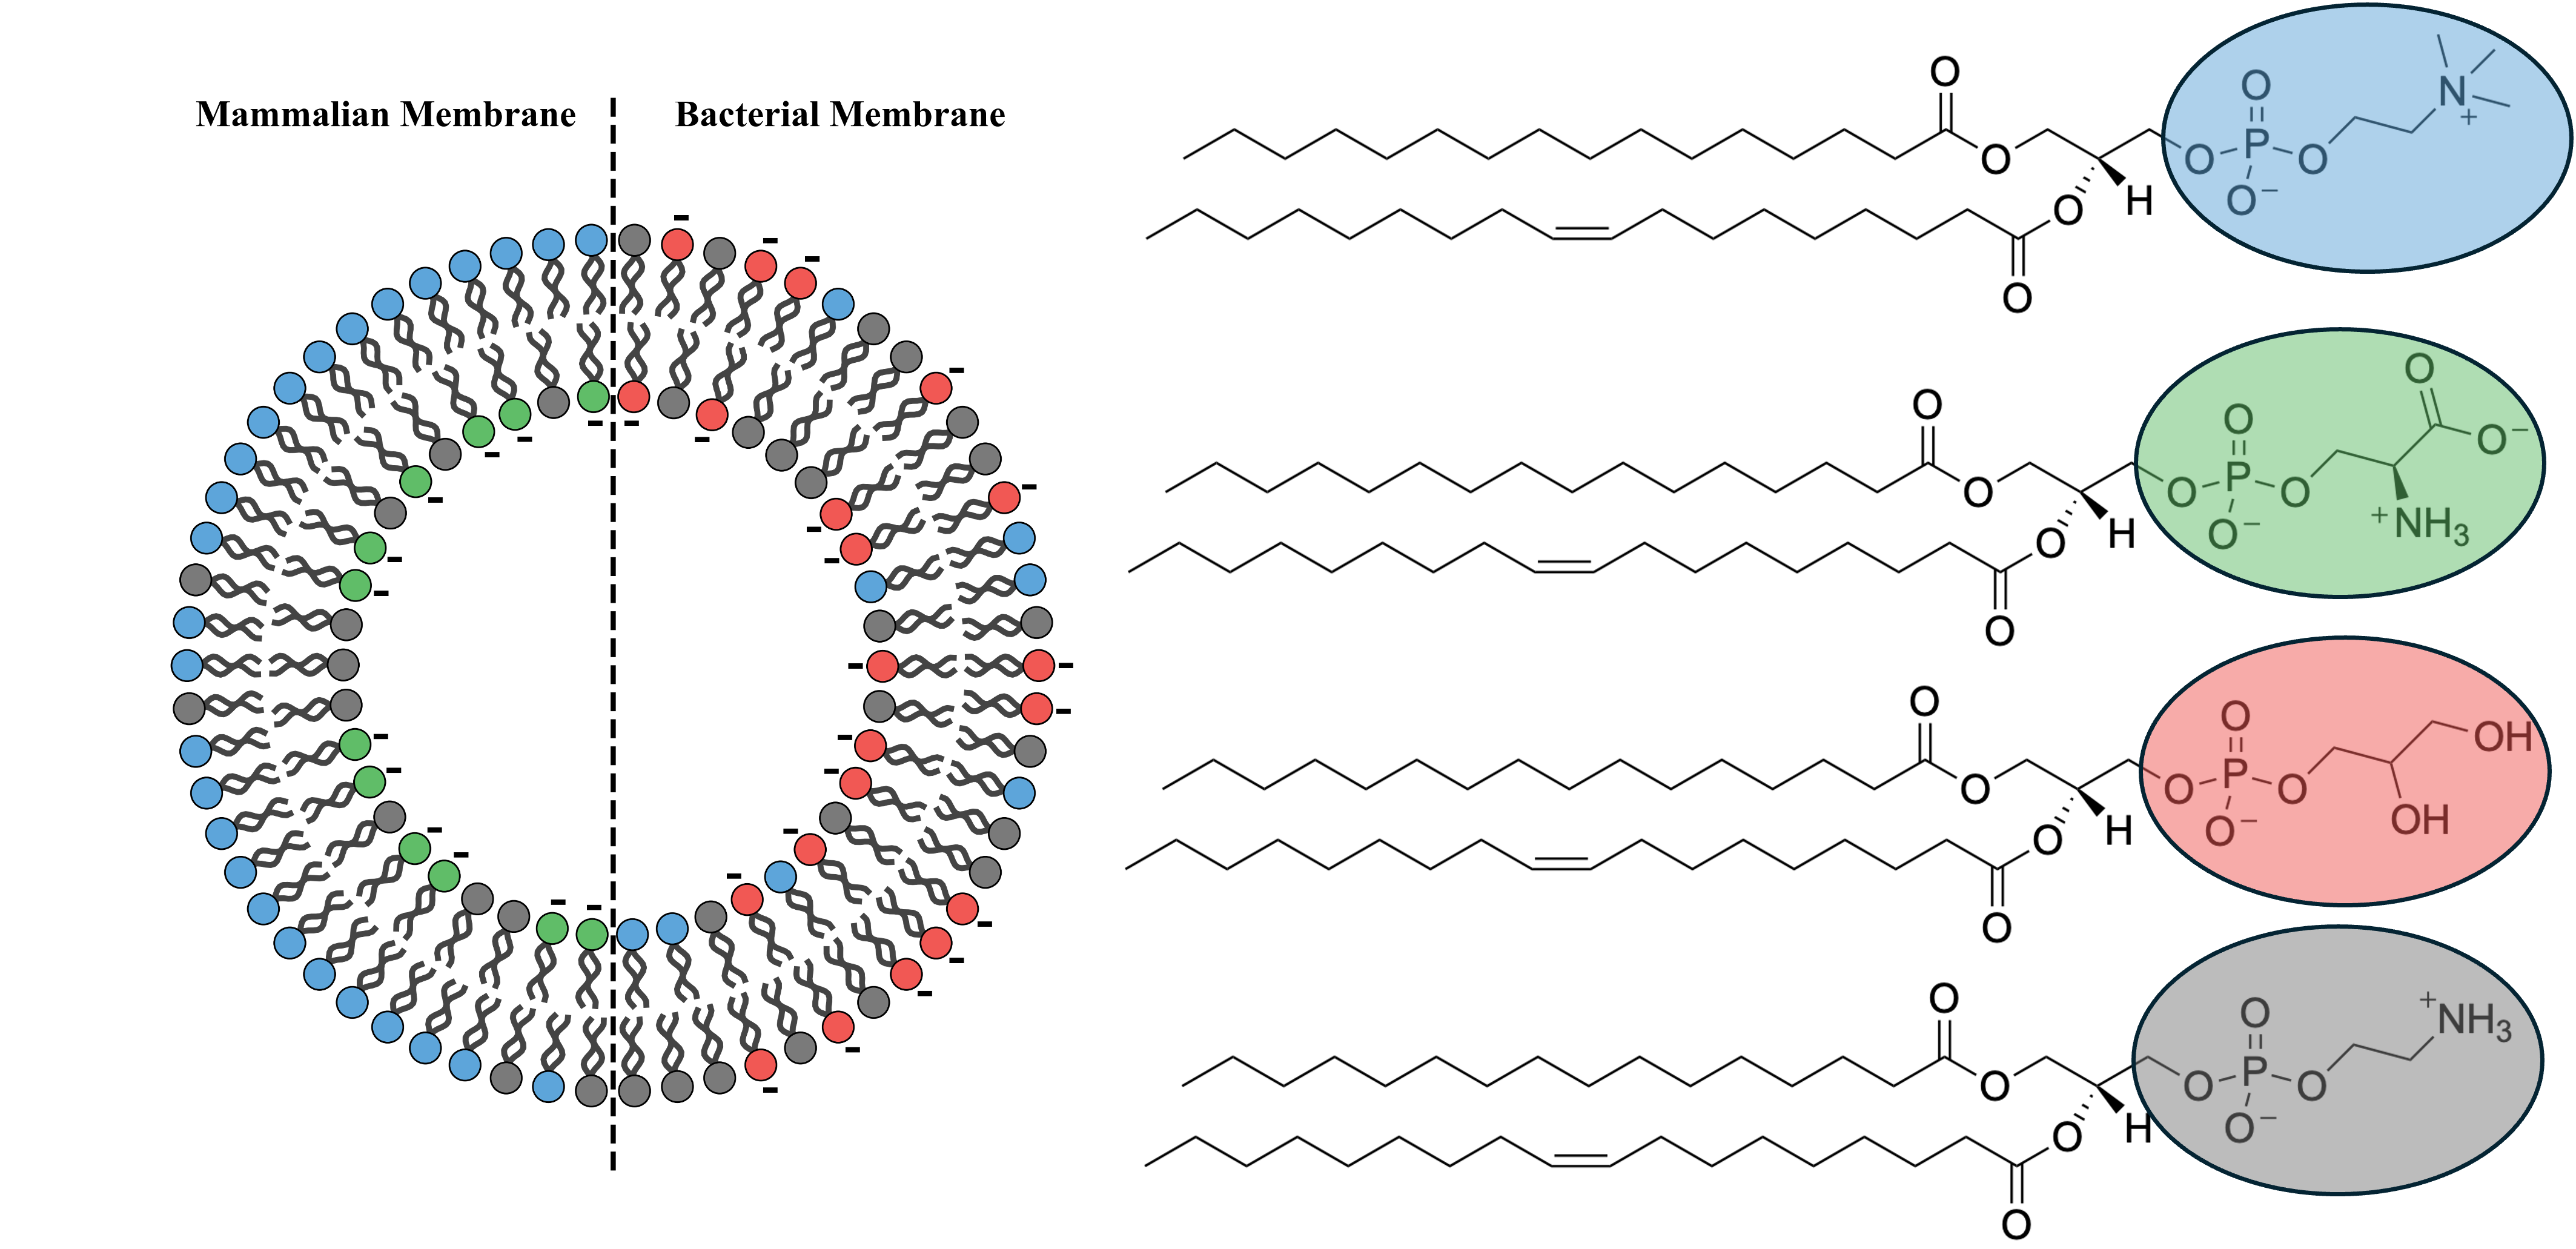
\includegraphics[width=0.95\linewidth]{General_Sections/Figures/Membrane_Lipids.png}
    \caption{The scheme in the left shows the comparison of the lipid composition of mammalian cells and bacteria membranes. In a healthy mammal, the membrane presents lipid asymmetric: the outer leaflet is primarily composed of neutral phosphatidylcholines (blue), while the inner leaflet is enriched with phosphatidylethanolamines (gray) and anionic phosphatidylserines (green), which provide a net negative charge. On the other hand, bacteria contain mainly---both in the interior and exterior leaflet---phosphatidylethanolamines and anionic phosphatidylglycerols (red) making them negatively charged. The structures in the right represent the most common lipids in eukaryotic and bacteria cells. From top to bottom DMPC, DMPS, DMPG, and DMPE. The left figure was created using Matplotlib, while the molecular structures were sketched with ChemDraw.}
    \label{fig:Lipids}
\end{figure}
\FloatBarrier

In the search for new antimicrobial strategies, nature provides an important source of inspiration. As part of their innate immune systems, many animals and plants produce antimicrobial peptides (AMPs) across a variety of tissues and cell types \cita{Zasloff2002}. These peptides have attracted particular interest due to their ability to exploit fundamental physicochemical differences between bacterial and eukaryotic membranes, and are often hypothesized to interact preferentially with membrane compositions enriched in negatively charged lipids\cita{Midura-Nowaczek2014}.

\section{Antimicrobial Peptides}
Antimicrobial Peptides are a class of small peptides that are widely found in nature. They exhibit structural and functional diversity and are active against Gram-positive and Gram-negative bacteria, fungi, parasites, and viruses \cita{Hancock2006}\textsuperscript{,}\cita{Kumar2018}. AMPs typically consist of 10 to 60 amino acids, and almost all AMPs are cationic, although several anionic AMPs have been reported, with up to 187 entries listed in the antimicrobial peptide database APD3 as of December 2024 \cita{Wang2016}. The diversity of AMPs makes their classification difficult, which can be based on: source, activity, structural characteristics, and amino acid-rich species (Figure \ref{fig:AMPClass})\cita{Huan2020}.
% \FloatBarrier
\begin{figure}[h]
    \centering
    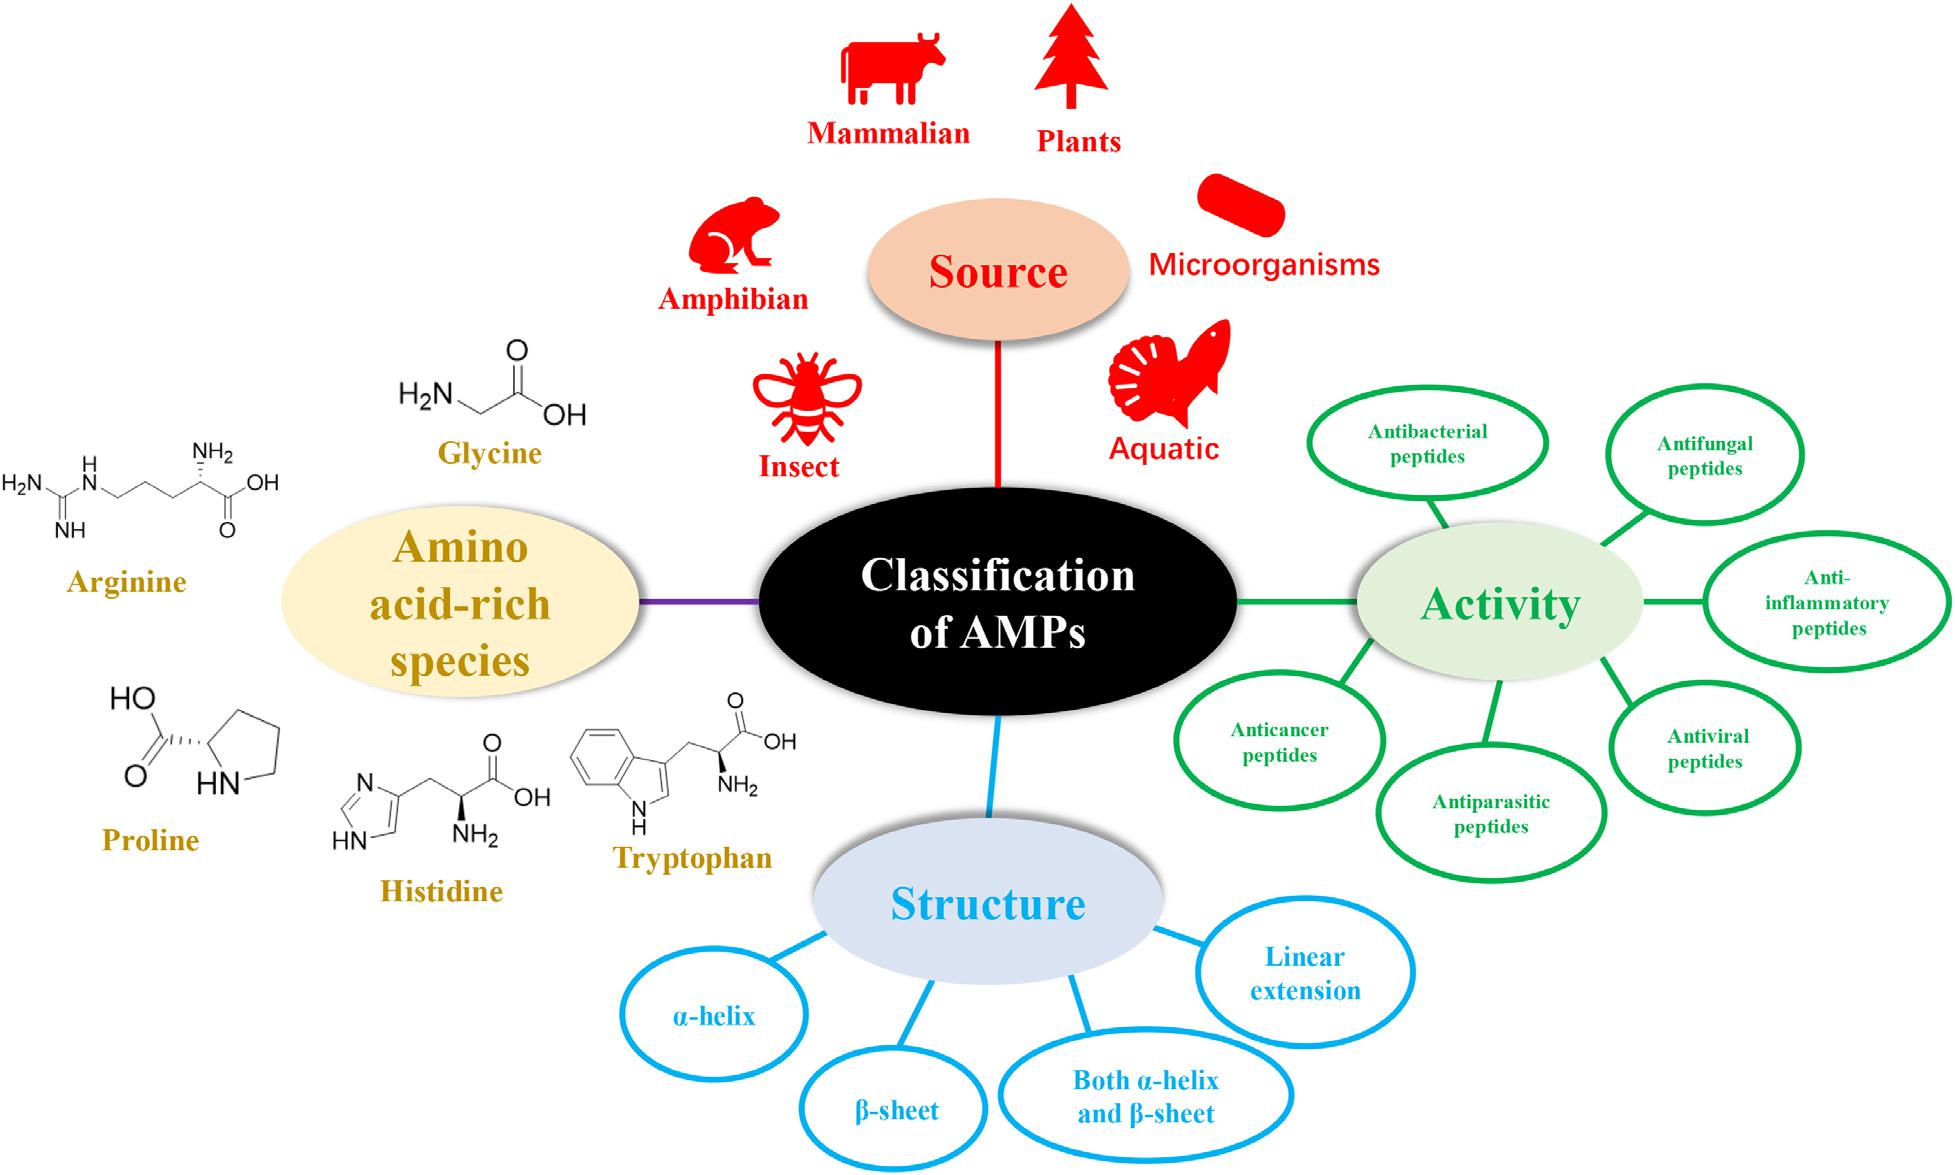
\includegraphics[width=0.8\linewidth]{General_Sections/Figures/AMP_Classification.jpg}
    \caption{Classification of Antimicrobial Peptides. Image taken from the work of Huan, Y. \textit{et al} under a Creative Commons License.}
    \label{fig:AMPClass}
\end{figure}
% \FloatBarrier

Their biological activity is commonly linked to their cationic nature, which allows electrostatic interactions with the negatively charged membranes of invading pathogens rather than with the neutrally charged membranes of eukaryotic cells \cita{Zhang2021}. Additionally, hydrophobicity---defined as the percentage of hydrophobic residues---is another key feature, as it influences the ability of AMPs to partition into membrane lipid bilayers \cita{Yeaman2003}. AMPs usually present a hydrophobicity of around 50\%, which, together with their cationicity, typically leads to amphipathic structures. In many cases, AMPs are largely unstructured in aqueous solution but undergo a conformational transition to $\alpha$-helical structures upon interaction with lipid membranes, a process that enhances their amphipathic character and membrane-disruptive potential \cita{Li2021}. While some AMPs display their antimicrobial activity by means of non-lytic mechanisms \cita{Scocchi2016}, the most common modes of action involve membranolytic effects driven by their amphiphatic nature (Figure \ref{fig:AMPMOA}). In a first stage, electrostatic interactions with negatively charged components of the membranes promote the accumulation of AMPs. Next, the membrane’s non-polar core interacts with the peptides’ hydrophobic residues, facilitating their insertion, disturbing membrane structure, and ultimately leading to cell death\cita{Mookherjee2020}\textsuperscript{,}\cita{BuiThiPhuong2024}.

\begin{figure}[h]
    \centering
    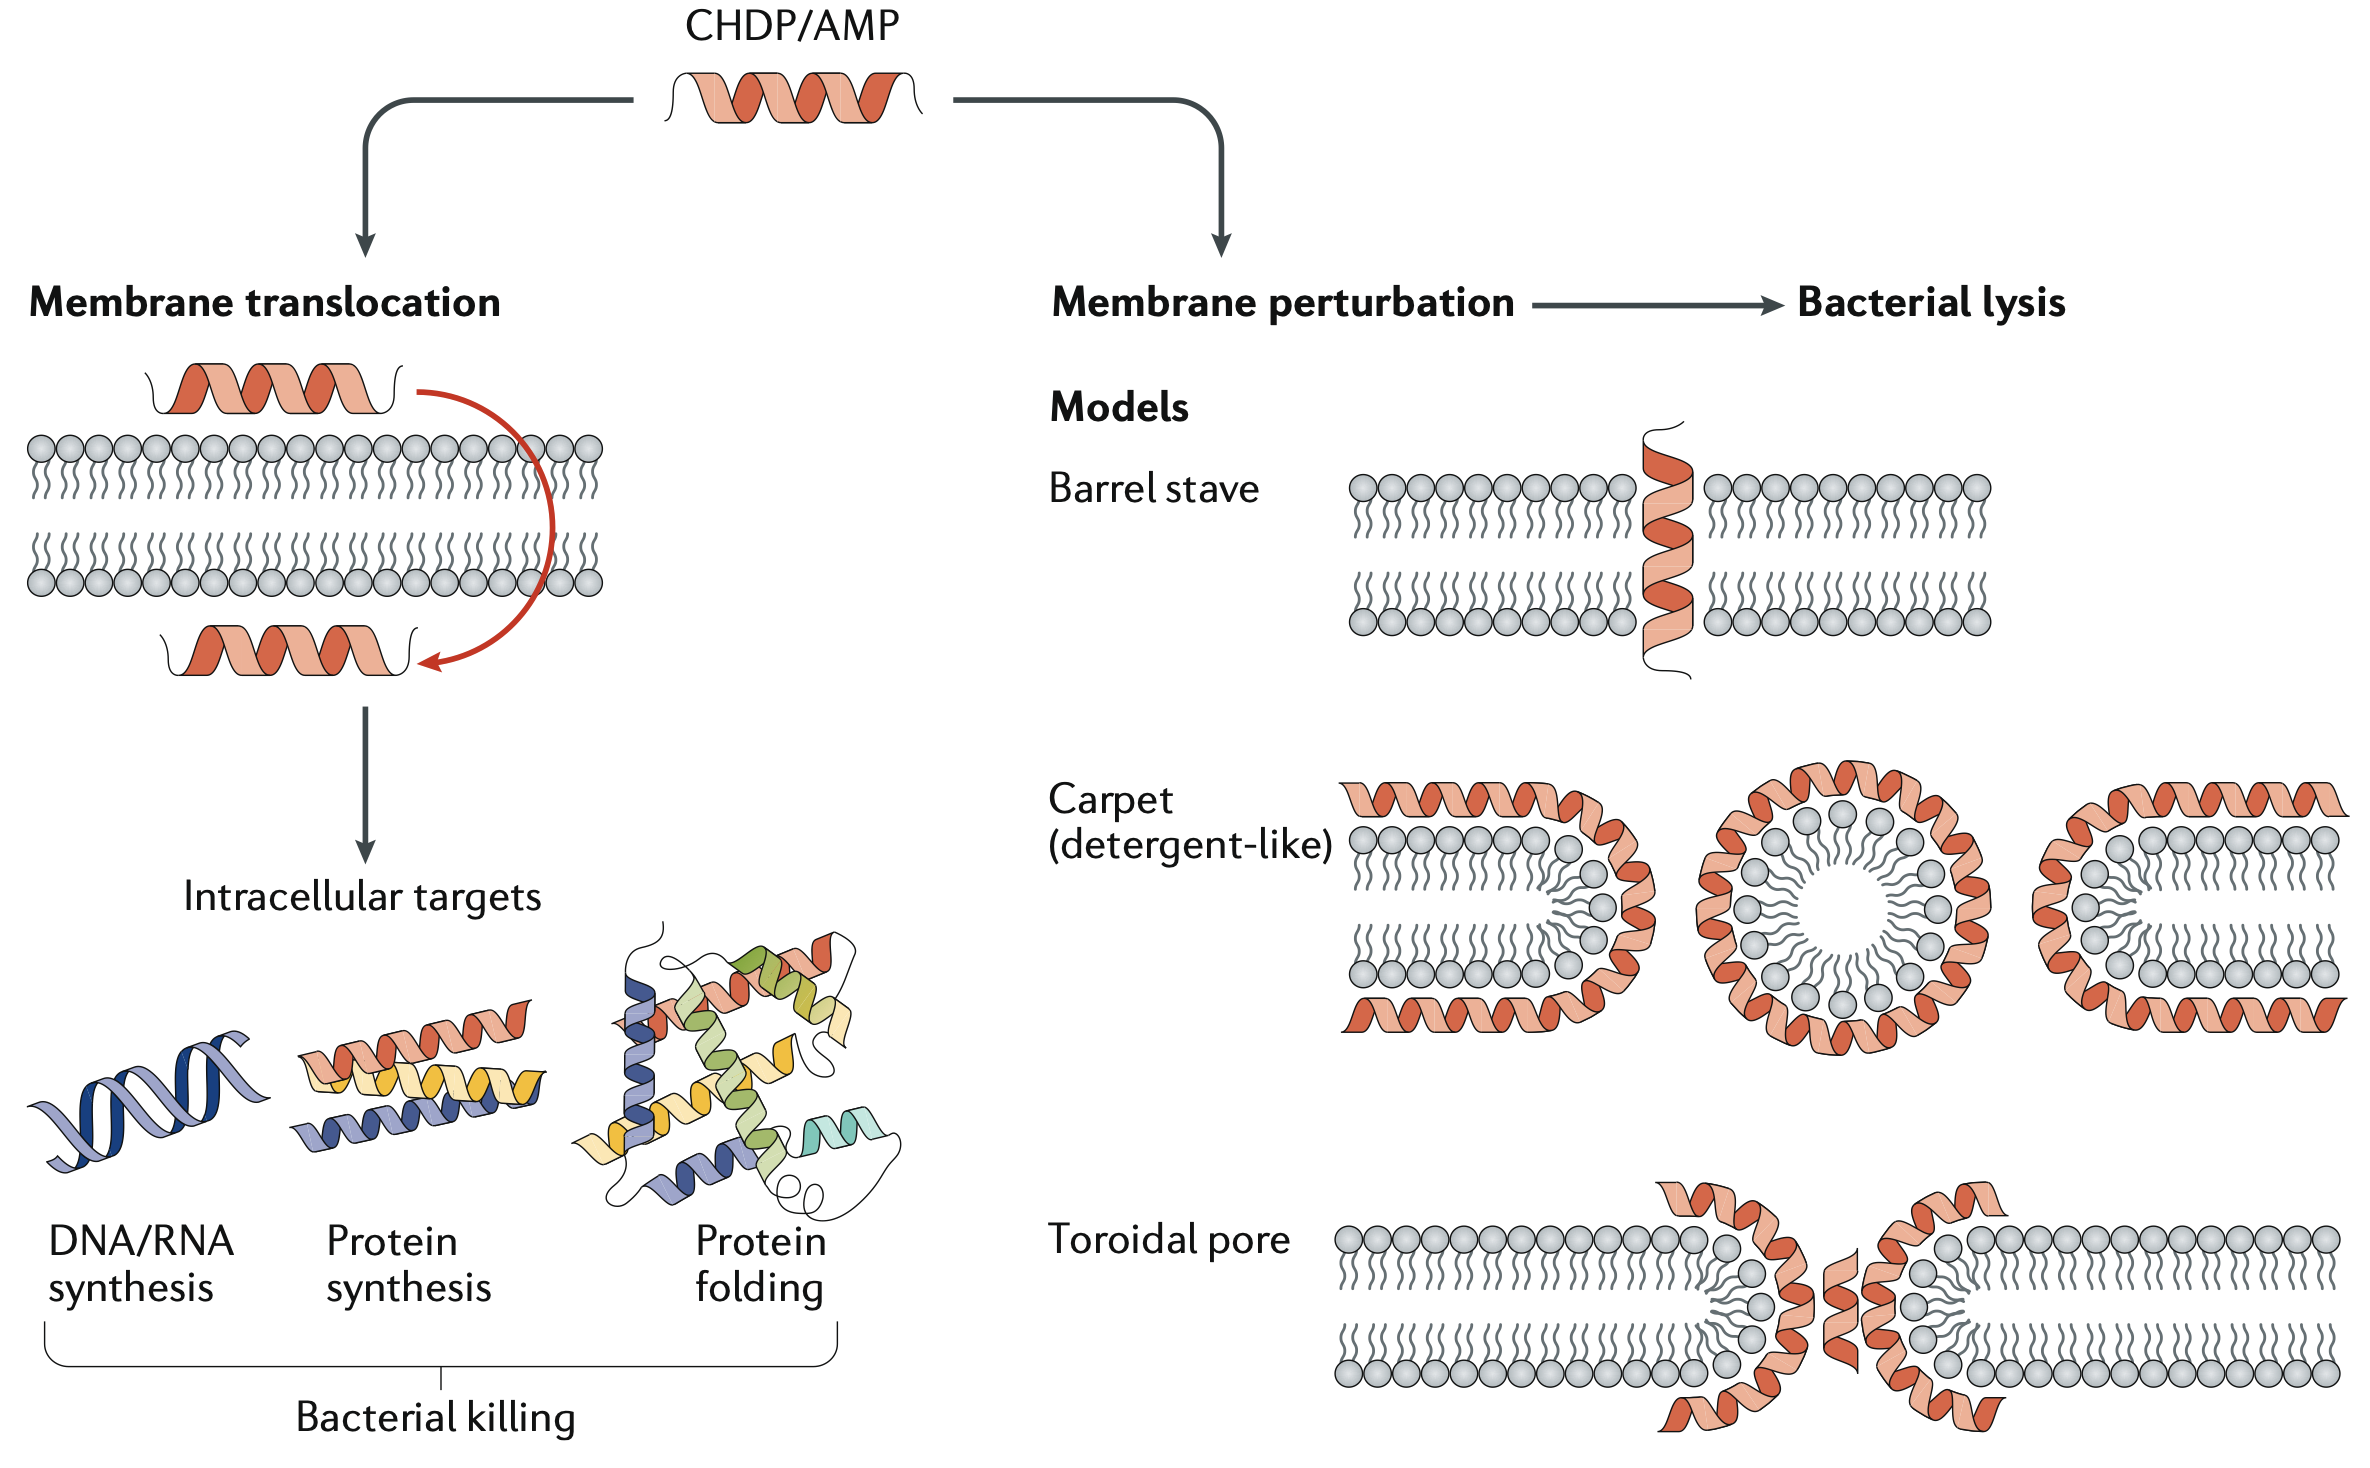
\includegraphics[width=0.69\linewidth]{General_Sections/Figures/AMPMOA.png}
    \caption{Indirect (non-lytic) and direct (membrane-related) mechanisms of bacterial killing proposed for AMPs. Image taken from the work of Mookherjee, N. \textit{et al}, copyright by Springer Nature.}
    \label{fig:AMPMOA}
\end{figure}
\FloatBarrier

As of its latest update in December 2024, the Data Repository of Antimicrobial Peptides (DRAMP)\cita{Ma2025} lists 35918 entries under the query "antimicrobial". Nevertheless, only a few AMPs have reached clinical trials, and just 80 peptide-based drugs have been approved worldwide\cita{Rossino2023}. A major limitation of AMPs is their metabolic instability, as they are rapidly degraded by proteolytic enzymes\cita{Dijksteel2021}. They also tend to exhibit toxicity toward host cells, which limits their therapeutic application\cita{Lyu2023}. In addition, they tend to have short half-lives and are quickly cleared from the bloodstream, which results in poor bioavailability. To overcome these limitations, various strategies have been investigated, such us incorporating non-natural amino acids and peptide cyclization to improve stability and minimize degradation\cita{Carmona2013}\textsuperscript{,}\cita{Lucana2021}.

In this context, there are already cyclic versions of AMPs that exhibit good activity \cita{Mika2011}\textsuperscript{,}\cita{Abraham2014}, highlighting CPs as a promising strategy to enhance natural AMPs or to design new sequences to mimic their function.
 
\section{Self-Assembled Cyclic Peptide Nanotubes}
Researchers, in their continuous effort to push the boundaries of science, have envisioned CPs not only as a means to improve AMPs, but also as promising building blocks for the formation of nanotubular structures driven by noncovalent interactions\cita{Chapman2012}. 

The first self-assembled cyclic peptide nanotubes (SCPNs) were synthesized by Ghadiri in 1993, almost 20 years after they were first proposed by De Santis in 1974\cita{Ghadiri1993}\textsuperscript{,}\cita{DeSantis1974}. These CPs were formed by an even number of alternating \textit{D-} and \textit{L-}$\alpha$-amino acid residues. The alternating chirality leads to a flat, ring-shaped molecule, leaving the oxygens of the carbonyl groups (C=O) and the hydrogens of the amine groups (NH) oriented perpendicular to the plane of the CP. This unique geometry allows CPs to self-assemble by forming hydrogen bonds (H-bonds) with adjacent CPs, mimicking a $\beta$-sheet arrangement (Figure \ref{fig:SCPN}A).

\begin{figure}[htbp]
  \centering

  % Top image (A)
  \begin{subfigure}{0.6\textwidth}
    \centering
    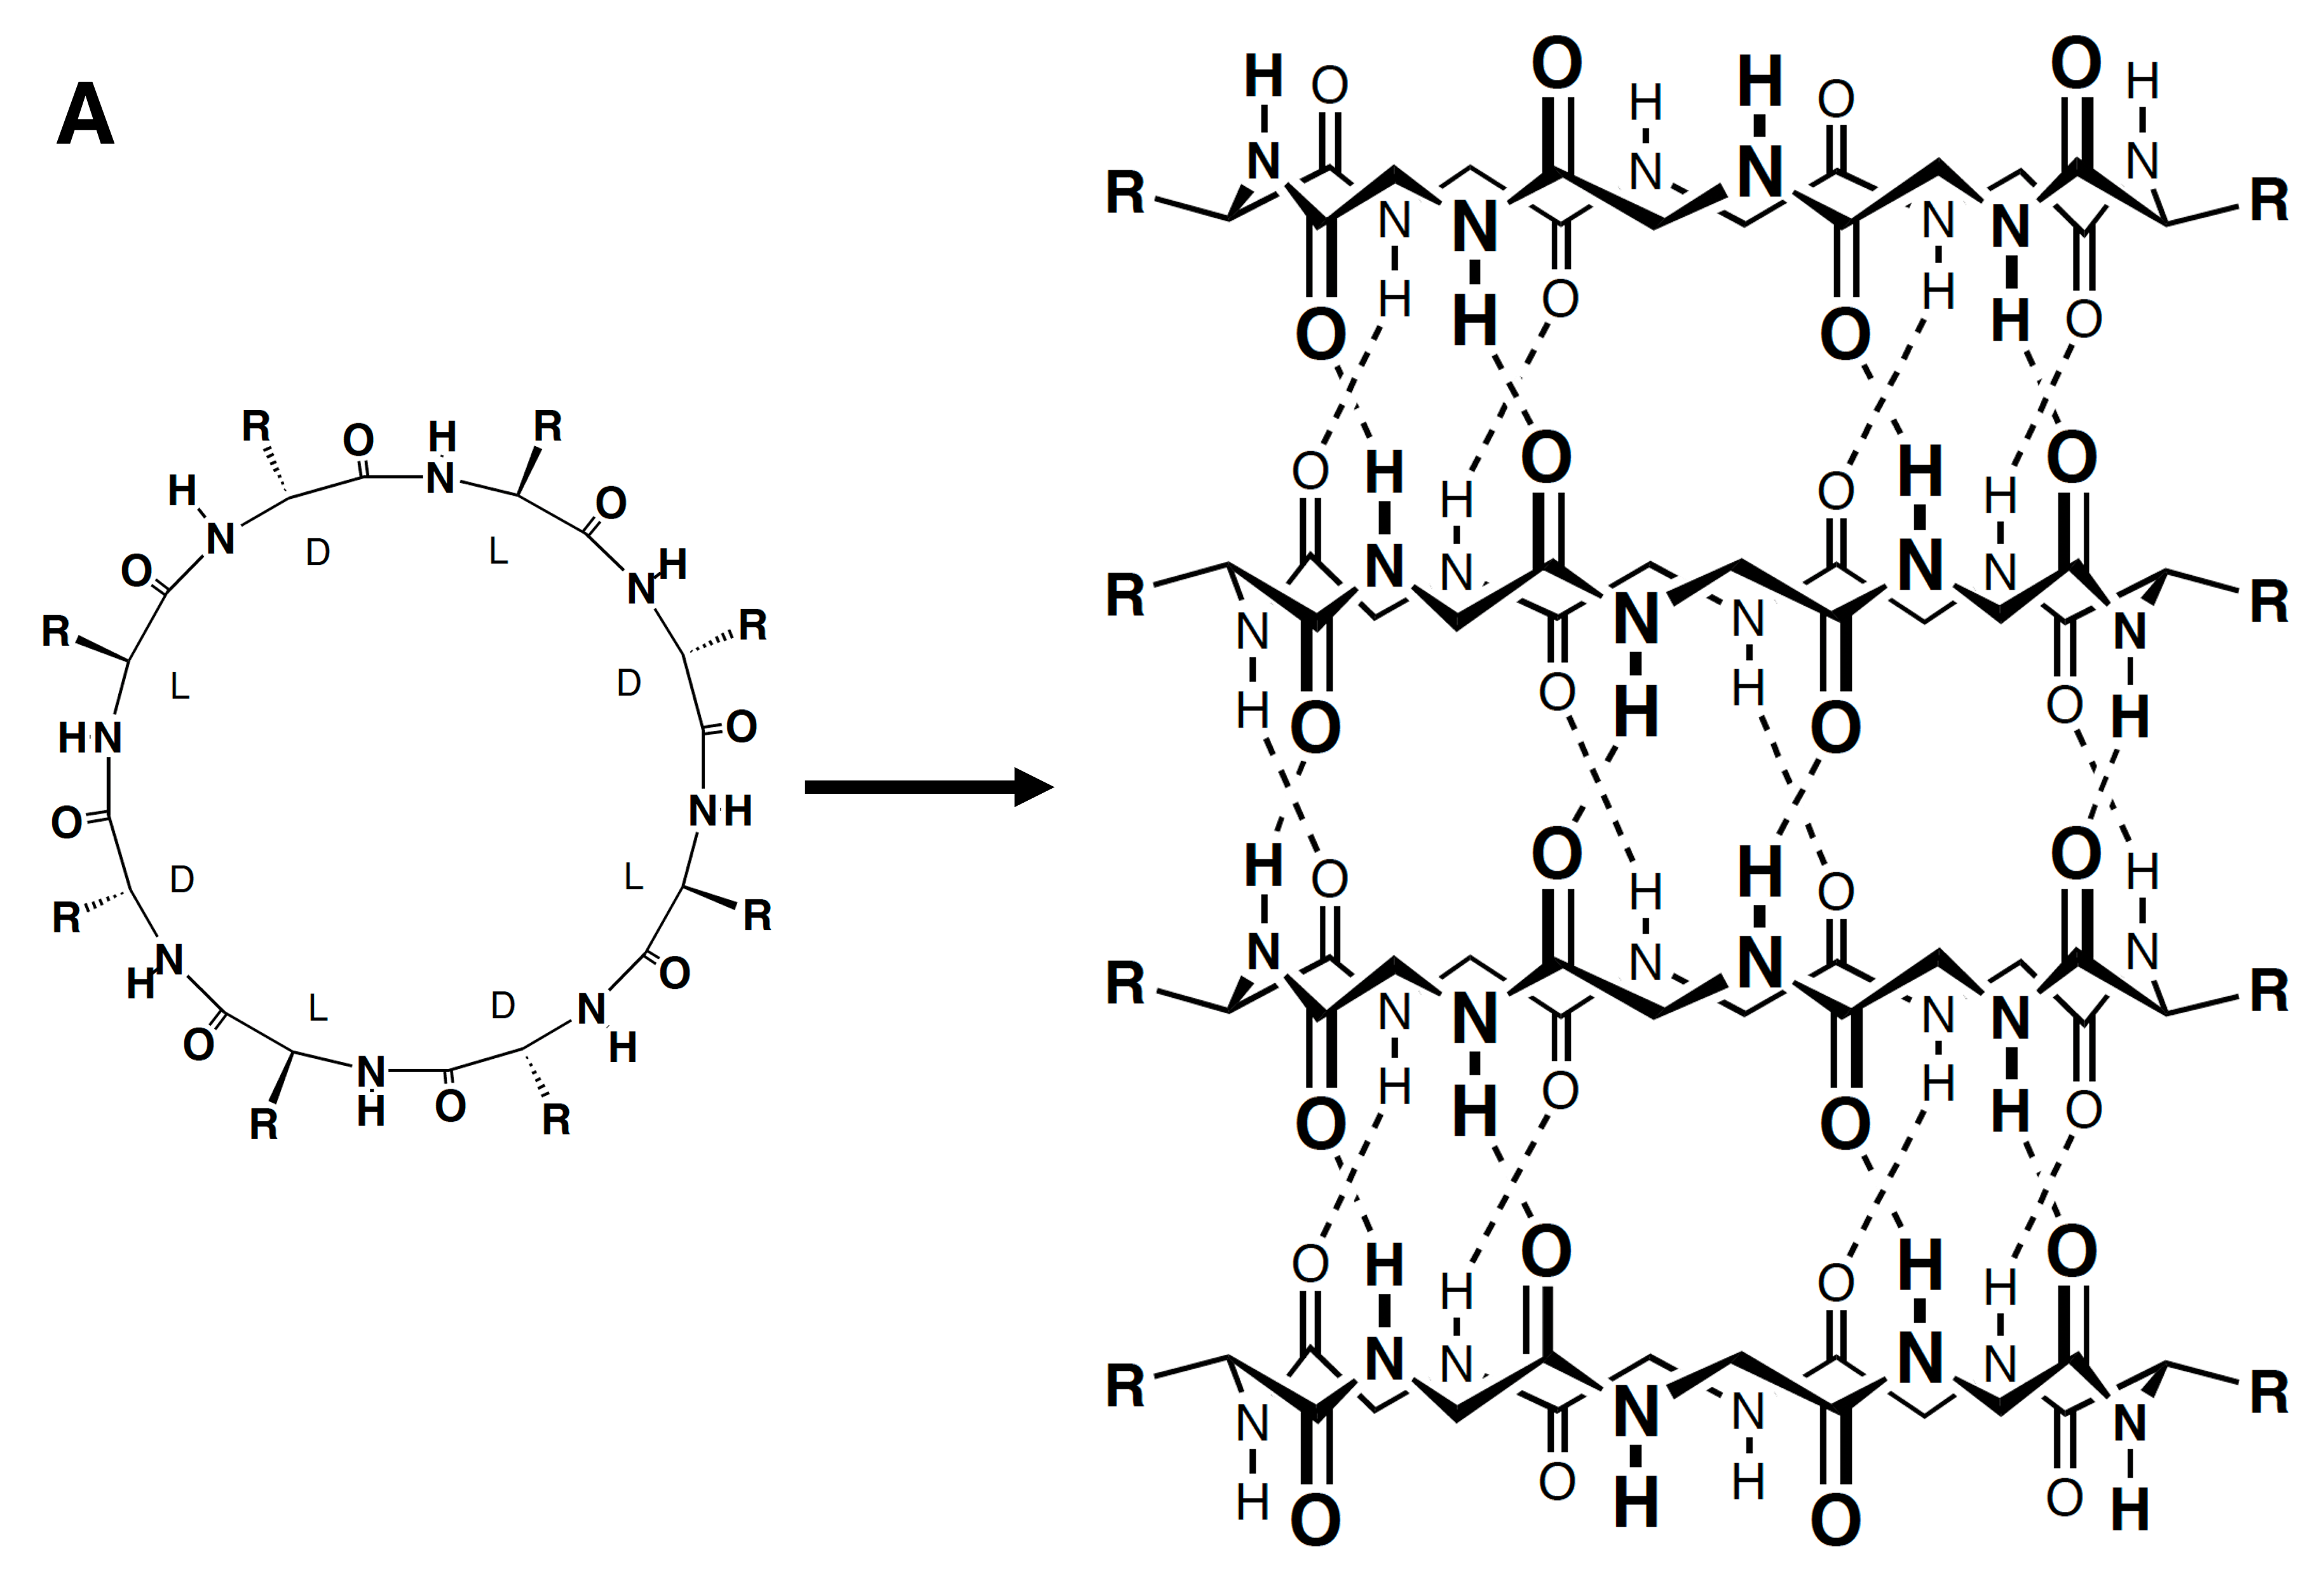
\includegraphics[width=\linewidth]{General_Sections/Figures/SchematicSCPN.png}
  \end{subfigure}

  % \vspace{1em} % vertical space between the two images

  % Bottom image (B)
  \begin{subfigure}{0.6\textwidth}
    \centering
    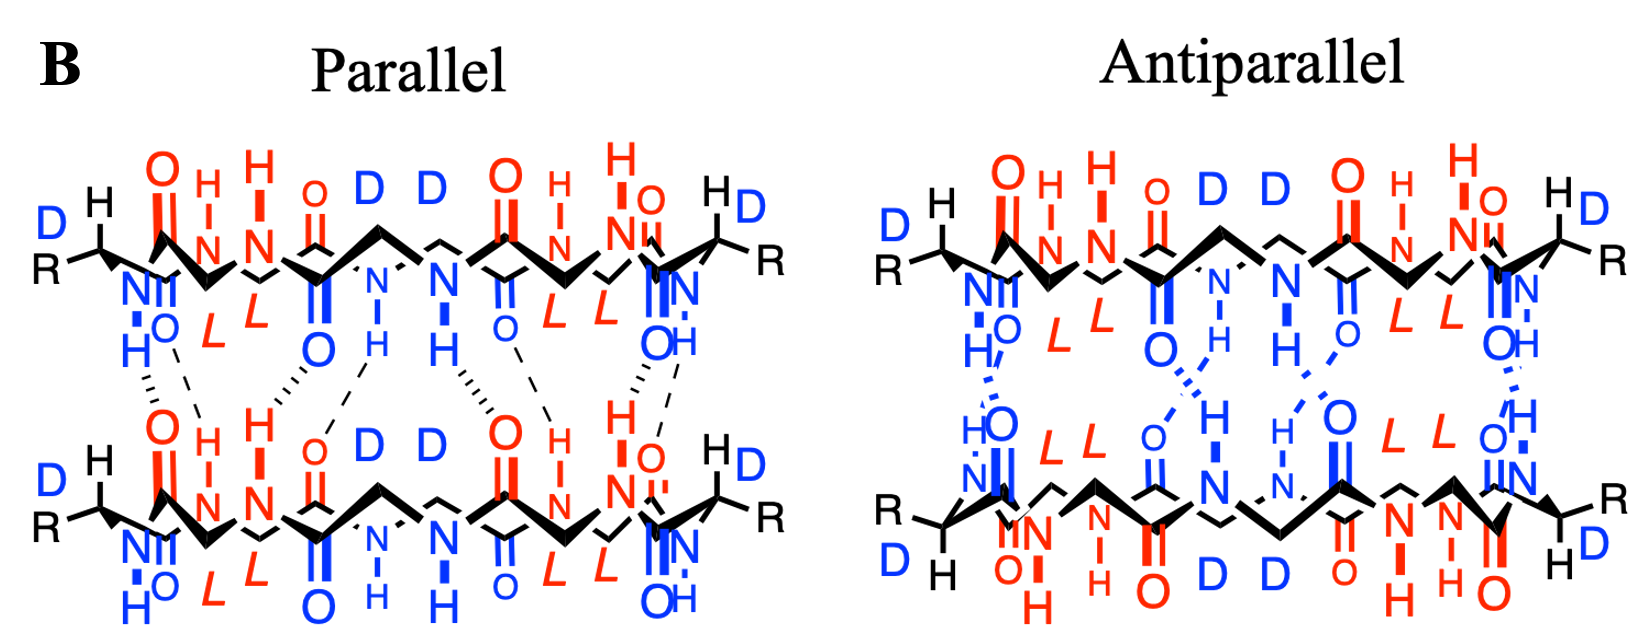
\includegraphics[width=\linewidth]{General_Sections/Figures/PvsA.png}
  \end{subfigure}

  \caption{\textbf{A} Schematic representation of a \textit{D,L-}$\alpha$-C and the corresponding assembly in a SCPN. \textbf{B} Representation of the parallel and antiparallel $\beta$-sheets formed by CPs.}
  \label{fig:SCPN}
\end{figure}

Furthermore, in this planar conformation, all the C=O and NH groups of residues with the same chirality point in the same direction, giving rise to two distinct faces: a \textit{D-}face and a \textit{L-}face. This allows two CPs to assemble by forming either parallel or antiparallel $\beta$-sheet-like structures (Figure \ref{fig:SCPN}B).

The resulting SCPNs have an internal cavity and an external surface, whose properties can be tailored during CP synthesis. The internal diameter can be adjusted by increasing the number of amino acids in the sequence. Moreover, hydrophobicity can be tuned by replacing some of the $\alpha$-residues with $\beta$-amino acids\cita{Claro2018} or $\gamma$-/$\delta$-cycloalkyl-like amino acids\cita{Amorn2003}\textsuperscript{,}\cita{Lamas2018}. In contrast, the nature of the external surface is determined by the choice of amino acids, and this has been observed to dictate the behaviour of the SCPNs in the presence of lipid bilayers, thereby shaping their applications.

In 1994, Ghadiri's group showed that CPs with hydrophobic side-chains, such as Leu or Trp, could self-assemble within lipid bilayers (Figure \ref{fig:Assembly}), forming transmembrane channels capable of ion transport \cita{Ghadiri1994}\textsuperscript{,}\cita{Kim1998}. Subsequent studies revealed that the use of amphipathic CPs with well differentiated hydrophobic and hydrophilic regions, could align parallel to the surface of the membrane (Figure \ref{fig:Assembly}), showing good antimicrobial activity \cita{Fernandez-Lopez2001}. These findings highlight the potential to tune SCPN-membrane interactions through CP sequence engineering.

\begin{figure}[h]
    \centering
    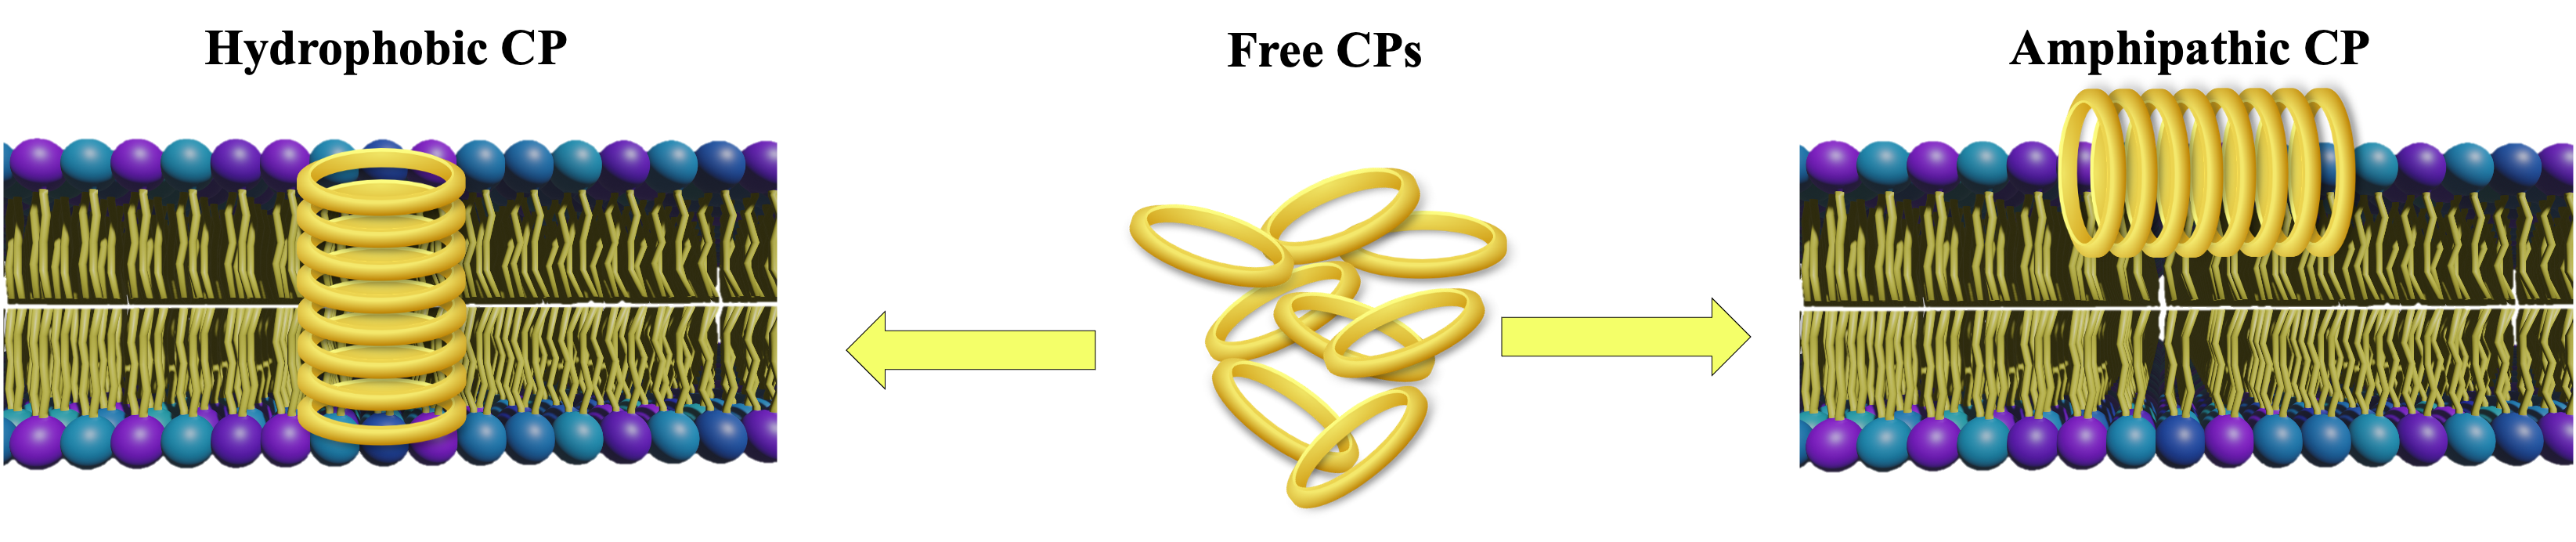
\includegraphics[width=0.9\linewidth]{General_Sections/Figures/DirectedAssembly.png}
    \caption{Representation of the disposition relative to the membrane adopted by hydrophobic SCPNs (left) and amphipathic SCPNs (right).}
    \label{fig:Assembly}
\end{figure}
\FloatBarrier

To effectively design SCPNs to exhibit specific properties or biological functions, it is important to decipher their mechanisms of action. This demands atomic-level resolution, which remains challenging for most experimental techniques. Furthermore, SCPNs---like other supramolecular systems---are highly dynamic. Thus, to fully understand the relationship between sequence, structure, and function, it is necessary to observe how these molecules interact with themselves and their environment in real time. Without the capability to understand the dynamic behavior and structural changes that define their activity, their design must rely on empirical approaches, as well as on serendipity. In this regard, computational techniques and, in particular, Molecular Dynamics (MD), have already proven to be useful tools to advance our understanding of SCPNs \cita{Moral2023}\textsuperscript{,}\cita{Insua2023}.

\section{Computational Methods in Chemistry}

As the performance of computational methods is tightly linked to the available computational power, advances in supercomputing and simulation techniques are pushing the boundaries of molecular simulations of biological systems. In parallel, the breakthrough of Artificial Intelligence (AI) is revolutionizing science, by enabling the analysis of huge databases to make accurate predictions. In the field of molecular biophysics and chemistry, MD simulations and ML approaches are increasingly recognized as complementary tools. While ML models have already demonstrated the ability to predict properties such as CP membrane permeability directly from experimental data \cita{Cao2024}\textsuperscript{,}\cita{Yu2024}, MD simulations provide a unique advantage by generating physically consistent, time-resolved trajectories that describe molecular structure, dynamics, and interactions under well-defined conditions. This makes MD-derived data particularly suitable for training and validating ML models, especially in systems where experimental characterization is challenging. This synergy between Molecular Dynamics and Artificial Intelligence is the main foundation of this doctoral thesis. By combining physics-based modeling with data-driven approaches, this work aims to bridge molecular-level mechanisms and predictive capabilities, contributing to emerging paradigms in computational chemistry.

\subsection{Molecular Dynamics}

MD is a simulation technique used to study the evolution over time of molecular systems by explicitly modeling the motion of atoms or interaction sites through the numerical integration of Newton’s equations of motion. At each time step, the forces acting on the particles are computed using force fields, a set of equations and parameters that describe different inter and intramolecular interactions \cita{Ciccotti2022}.

The first MD simulation dates back to 1957, when Wainwright and Alder simulated systems of hard spheres using a discontinuous potential \cita{Alder1957}. The next step was taken by Rahman in 1964, who simulated liquid argon using a Lennard-Jones pairwise additive potential to account for the interactions between argon atoms. During an era in which computers were scarce and limited in speed and memory, advances in algorithms were essential. In 1967, for example, Verlet proposed a stable numerical integration scheme for Newton's equations, an approach that is still widely used today \cita{Verlet1967}. Later on, in 1971, Rahman and Stillinger published for the first time an MD study on a model of liquid water \cita{Rahman1971}, demonstrating that its structure is formed by a dynamic network of hydrogen bonds. Although today this may seem like routine work, at the time it led the scientific community to believe that if it was possible to simulate water, the medium of the chemistry of life, why not simulate biomolecules themselves? The breakthrough came in 1977, when a group led by Karplus published the first MD simulation of a simple protein \cita{McCammon1977}.

During the early 1980s significant progress was made in developing algorithms to sample conditions relevant to experiments. Standard MD simulations operate in the microcanonical (constant energy) ensemble, since Newton's equations of motion conserve the total energy. Andersen was the first to propose a method for achieving constant-pressure MD simulations by extending the dynamical variables of the system to include the volume \cita{Andersen1980}. He was later followed by Parrinello and Rahman, who extended the scheme to include shape fluctuations as well \cita{Parrinello1980}\textsuperscript{,}\cita{Parrinello1981}. Building on Andersen's work, Nosé introduced a new dynamical variable, coupling the kinetic energy of the atoms to the external temperature, allowing MD to sample the canonical ensemble \cita{Nose1984}. Hoover later refined this approach leading to what is known as Nosé-Hoover thermostat \cita{Hoover1985}, widely used in MD simulations today.

Since then, both the size of the simulated systems and the simulation times have grown exponentially, making it common to find studies in the literature on proteins, DNA/RNA complexes or self-assembly processes such as micelle formation \cita{Karplus2002}\textsuperscript{,}\cita{Sponer2018}\textsuperscript{,}\cita{Morrow2013}. More broadly, the impact of molecular simulation approaches on chemical research was formally recognized with the award of the 2013 Nobel Prize in Chemistry to Martin Karplus, Arieh Warshel and Michael Levitt for "the development of multiscale models for complex chemical systems".
%%%
Within this broader landscape, MD simulations have also been applied to the study of cyclic peptides (CPs) and self-assembled cyclic peptide nanotubes (SCPNs), providing molecular-level insight into their conformational behavior, self-assembly mechanisms, and interactions with lipid membranes. Atomistic MD studies offer a level of structural and dynamical detail difficult to access experimentally, helping to elucidate how peptide sequence, chirality, and amphipathicity influence supramolecular organization. Despite these capabilities, previous research in our group has focused specifically on embedded nanotubes, investigating their stability and implications for membrane structure \cita{GF2016}\textsuperscript{,}\cita{Calvelo2019}\textsuperscript{,}\cita{Xandre2021}\textsuperscript{,}\cita{Conde2022}. A shared feature of the cited works was the use of pre-assembled nanotubes that were manually inserted into lipid bilayers, a necessity driven by the high computational cost of the application of atomistic MD to CP and SCPN systems. Key processes such as peptide self-assembly, membrane insertion, and supramolecular rearrangement typically occur on microsecond to millisecond timescales and involve large peptide–membrane assemblies, placing them beyond the practical reach of routine atomistic simulations.

To overcome these limitations, coarse-grained (CG) Molecular Dynamics approaches have been increasingly adopted, as they enable the simulation of larger systems over longer timescales. CG models have been successfully applied to study the interactions of various CP sequences with lipid bilayers, starting either from a pre-assembled nanotube in solution or from randomly positioned units that self-assemble \cita{Claro2020}\textsuperscript{,}\cita{Claro2021}. However, while CG models are well suited to capture collective phenomena such as aggregation and membrane remodeling, their reduced resolution often compromises the accurate description of direction-specific interactions, including hydrogen-bond networks, backbone geometry, and chirality-dependent stacking. These features are particularly critical for CPs and SCPNs, whose self-assembly is governed by highly directional hydrogen bonding and precise geometric constraints. As a result, existing CG force fields may fail to faithfully reproduce key aspects of cyclic peptide self-assembly and membrane interactions, despite their favorable computational efficiency.

This gap between atomistic accuracy and CG scalability highlights the need for computational strategies that preserve essential structural features of cyclic peptides while enabling systematic, large-scale simulations and data-driven analysis.

Looking forward, MD continue to benefit from advances in high-performance computing, including the deployment of exascale architectures, which enable increasingly large and long simulations of complex molecular systems. In parallel, the breakthrough of AI, and in particular Machine Learning (ML), is profoundly revolutionizing the field. Beyond their application as classification or prediction tools, ML-based approaches are increasingly integrated into the core of theoretical chemistry through the development of ML potentials, which offer a promising route to accelerate MD while preserving atomic accuracy.


\subsection{Machine Learning}\label{ML_intro}
%%%%%% CONTINUE
Although commonly confused in everyday conversations, AI and ML refer to distinct but interconnected concepts. AI describes the field of study dedicated to enabling computers and machines to simulate human intelligence and capabilities, performing tasks such as reasoning or decision-making. ML constitutes a major subfield of AI, concerned with developing models by training algorithms to make predictions based on data rather than explicitly programming them to provide an outcome.

The term Machine Learning was coined by Arthur Samuel in the late 1950s, when his computer program for playing checkers was one of the first successful self-learning programs \cita{Samuel2000}. In parallel, Frank Rossenblatt, inspired by Donald Hebb's model of brain cell interaction \cita{Hebb2005}, developed a simple neuron-inspired classifier called the perceptron \cita{Rosenblatt1958}. The software was installed in a custom-built machine called the Mark I Perceptron, which had been constructed for image recognition. Despite early promise, its limitations in recognizing some visual patterns led to disappointment and temporarily stalled progress in neural network research.

A resurgence came in the 1980s as the development of new training algorithms and increased computational power unlocked multi-layer neural networks. In 1986, Rumelhart, Hinton, and Williams popularized the back-propagation algorithm that enabled networks to adjust internal weights in hidden layers, learning feature representations beyond the perceptron's reach \cita{Rumelhart1986}. In the 1990s, Hochreiter and Schmidhuberthe developed the Long Short-Term Memory (LSTM) networks that addressed the long-standing vanishing gradient problem that was burden recurrent networks. LSTMs soon achieved state-of-the-art performance on sequential data tasks, breaking records in domains like language modeling and machine translation by the mid-2010s \cita{Hochreiter1997}. By 2017, the confluence of large datasets and Graphics Processing Unit (GPU) computing led to the development of AlexNet, a deep convolutional neural network that scored a landmark victory in the ImageNet recognition challenge \cita{Krizhevsky2017}.

As ML matured, it increasingly intersected with other areas of knowledge like chemistry. For instance, in 2007 Behler and Parrinello showed that a neural network could replicate density functional theory (DFT) potential energy surfaces, providing energies and forces orders of magnitude faster than DFT calculations \cita{Behler2007}. Since then, ML potentials have gained popularity, as they are believe to extend accessible time-scales without sacrificing accuracy. Nevertheless, the most striking example of ML's impact on chemistry has arguably been in protein structure prediction. Predicting protein's 3D structure just based on the amino acid sequence remained unsolved for five decades. In 2020, DeepMind launched AlphaFold2, a neural network capable of predicting protein structures with unprecedented accuracy \cita{Jumper2021}. In recognition, the 2024 Nobel Prize in Chemistry was awarded to Demis Hassabis and John Jumper, creators of AlphaFold, as well as David Baker for his pioneering contributions to computational protein design. This was the first time an AI-driven scientific achievement earned a Nobel Prize, reinforcing that ML is no longer just a computational aid, but an essential tool for advancing chemical research.

In the context of medicinal chemistry and peptide research, ML approaches have been widely employed to predict biological activity, toxicity, and membrane permeability directly from experimental data \cita{Manavalan2018}\textsuperscript{,}\cita{Wang2024}\textsuperscript{,}\cita{Li2024}. Several models have been reported to infer cyclic peptide membrane permeability or antimicrobial activity from sequence-based representations or molecular descriptors, demonstrating the potential of ML to accelerate screening and guide peptide design \cita{CyclePermea}\textsuperscript{,}\cita{Feller2025}\textsuperscript{,}\cita{Tan2024}. However, ML models trained exclusively on experimental datasets often face important limitations. Experimental data is frequently scarce, heterogeneous, and biased toward specific chemical families, which can hinder model generalization and limit interpretability. Moreover, purely sequence-based representations may fail to capture key aspects of molecular behavior that arise from the three-dimensional structure, supramolecular organization, and dynamic interactions with complex environments such as lipid membranes.

In this context, Molecular Dynamics simulations offer a complementary and highly valuable source of training data for ML models \cita{Hui2023}\textsuperscript{,}\cita{Cherednichenko2025}\textsuperscript{,}\cita{Hui2025}. MD provides physically consistent, time-resolved information that encodes not only static structural features but also dynamic, thermodynamic, and interaction-based descriptors. By extracting quantitative features from MD trajectories, it becomes possible to generate large, homogeneous datasets that reflect underlying molecular mechanisms rather than purely empirical correlations.

The integration of ML with MD simulations opens new opportunities for bridging molecular-scale mechanisms and macroscopic observables. ML models trained on simulation-derived descriptors can learn complex relationships between sequence, structure, dynamics, and function, enabling rapid prediction and classification at a fraction of the computational cost of explicit simulations. For cyclic peptides and self-assembled cyclic peptide nanotubes, this combined MD–ML framework is particularly attractive, as it provides a route to explore vast sequence spaces while accounting for the supramolecular and membrane-associated phenomena that govern biological activity.


\section{Dissertation Structure}

This PhD dissertation is structured into seven main sections and one supplementary section. The manuscript first delves into the context behind the work, namely, the challenge of AMR, and then presents the molecules and techniques used to address it. After that, the objectives of this research are presented, followed by a technical explanation of the materials and methods used to carry out research. Subsequently, the scientific results are presented as a compendium of articles, comprising the five most relevant publications related to this thesis divided in three results sections. Finally, the contributions are discussed as a whole in order to draw a general list of conclusions. In particular, the document is structured as follows:
\begin{itemize}
    \item \textbf{Introduction}: The present section. It introduces AMR and proposes CPs as potential candidates to overcome it. Additionally, it also describes the scientific challenges of experimental CP research and provides an overview of the two main techniques used in this work: MD simulations and ML methods. 
    \item \textbf{Hypothesis and Objectives}: This section sets the main hypothesis that drive the research conducted in this thesis. Moreover, it provides a detailed description of the objectives that have to be achieved to test the proposed hypothesis.
    \item \textbf{Materials and Methods}: This section describes in detail the computational tools used in this research. It first focuses on MD, providing technical insights into the physical foundation and the force field, a pivotal aspect of the thesis. Then, it delves into Machine Learning, describing the main unsupervised and supervised methods featured in the published work.
    \item \textbf{Results: Published Articles}: This section includes the articles published during the thesis and, when applicable, the corresponding supporting information right after the article. Moreover, this section presents the platform CYCLOPEp, which contains registered code. The corresponding registration form is attached at the end of the article presenting \hyperlink{registro}{CYCLOPEp Builder}, the first tool of CYCLOPEp. The articles are in the original format they were published, including then, the discussion of the results obtained in each research work. Two sections form this chapter; Section \ref{chap1} covers the development of the MA(R/S)\-TINI force field and the creation of CYCLOPEp Builder, an online platform for the creation of CPs and SCPNs for MD simulations; Section \ref{chap3} describes a model trained to predict experimental CP membrane permeability, the results, and the different strategies tested to improve the accuracy.
    \item \textbf{Unpublished Results}: This section encompass the work that could not be published before the presentation of the thesis. Section \ref{chap2} includes the manuscript were CYCLOPEpDB, an in house database of CP-MD simulations, was presented. This article-like manuscript also provides ML results on the prediction of CP-Membrane interactions derived from the MD results. Although this section was placed after the one containing the published articles, the manuscript that it contains was originally intended to be placed between sections \ref{chap1} and \ref{chap3}, since it uses the tools of the former and advances the application of Machine Learning to Molecular Dynamics data before moving to experimental sources. Therefore, throughout all the thesis, it will be treated as if it was a work in between the aforementioned results sections. The supplementary information of this articles is also provided right after.
    \item \textbf{General Discussion}: This section includes a general overview of the results achieved in this thesis, highlighting the main outcomes of each article and how they integrate in the general purpose of this research.
    \item \textbf{Conclusions}: Presents a summary of the key conclusions drawn from the research carried out in this thesis.
\end{itemize}

\newpage

% Objectives
\chapter{Hypothesis and Objectives}
\chapterquote{Always look forward, keep your eyes on the goal, and do not stop until you reach it!}{All Might, My Hero Academia}


\newpage
\section{Hypothesis}

Because the molecular mechanisms underlying AMP function occur at complex interfaces, their transient and dynamic nature makes the precise characterization of these membrane-disrupting processes a significant experimental challenge\cite{hypothesis,srm_methods}. In this context, unbiased molecular dynamics (MD) and enhanced sampling techniques\cite{opes,steered_md,umbrella_sampling}, such as metadynamics\cite{Barducci2008}, provide a powerful complementary approach\cite{hypothesis}, offering precise atomistic and thermodynamic insights into how peptide orientation, specifically tilt and spin angles, drives selective membrane recognition and lipid assembly integration.  

A second hypothesis underlying this work is that the combinatorial explosion inherent to interfacial peptide folding and environment-conditioned sequence design; a problem characterized by a vast, high-dimensional space of potential solutions\cite{Levinthal_paradox,Levinthal_paradox_2}; can be effectively addressed through the application of Quantum Computing (QC)\cite{biology_quantum_computing,robert2021resource,perdomo_1,perdomo_2}. Classical computational approaches often struggle with the exponential scaling required to exhaustively explore these immense sequence and conformational landscapes\cite{biology_quantum_computing}. To overcome this fundamental bottleneck, this thesis posits that formulating the problem via physics-based Hamiltonian models allows the complex energetic landscape to be mapped into compact binary encodings. This quantum-ready framework enables the deployment of emerging hybrid quantum-classical algorithms, such as the Variational Quantum Eigensolver (VQE)\cite{peruzzo2014variational} and the Quantum Approximate Optimization Algorithm (QAOA)\cite{farhi2014quantum}. By leveraging these quantum techniques, it is possible to navigate the astronomical number of potential solutions more efficiently than classical exact enumeration, thereby accelerating the rational design of novel AMPs with tailored environmental specificity.


\section{General and specific Objectives}
Driven by these hypotheses, the overarching objective of this doctoral thesis is to decipher the molecular determinants that govern the sequence-structure-function relationships of $\alpha$-helical antimicrobial peptides (AMPs). Ultimately, this research aims to predict their interfacial folding dynamics and selective affinity for pathological lipid membranes, specifically those implicated in the Cancer-Aging-Infection (CAIn) triangle. To systematically achieve this goal, the work was structured around the following specific objectives:

\begin{enumerate}[font=\bfseries]
    \item \textbf{Systematic biophysical characterization of AMP-membrane interactions.} Previous studies often lack a detailed thermodynamic and mechanistic description of how AMPs insert into varying lipid environments[cite: 3]. The first objective of this thesis was to employ unbiased molecular dynamics (MD) and well-tempered metadynamics to decode the interaction of canonical AMPs (e.g., LL-37, magainin-2, pleurocidin) with distinct lipid bilayers mimicking healthy mammalian, bacterial, and cancerous cells[cite: 3]. This involved calculating accurate Free Energy Surfaces (FES) and determining the decisive role of the transverse hydrophobic dipole moment, tilt, and spin angles in governing peptide insertion and orientation[cite: 3]. This objective establishes the biophysical foundation of the thesis and is addressed in the first publication presented in chapter \ref{chap1}.
    
  
    
    \item \textbf{Implementation of peptide folding and design algorithms on Quantum Computers.} To overcome the exponential scaling bottlenecks of classical exhaustive enumeration for sequence design and structural prediction, the third objective focused on translating the developed physical models into quantum-compatible formats[cite: 1, 4]. This involved mapping the environment-conditioned Hamiltonian into a compact binary encoding and utilizing a tetrahedral lattice model[cite: 1, 4]. Subsequently, hybrid quantum-classical algorithms, such as the Variational Quantum Eigensolver (VQE) and the Quantum Approximate Optimization Algorithm (QAOA), were successfully applied to predict the optimal folding conformations of peptides explicitly positioned at the smooth interface between polar and non-polar media, and to optimize sequences[cite: 1, 4]. This objective pushes the boundaries of current computational biophysics by embracing emerging technologies, and is presented in the third publication in chapter \ref{chap2}.
    
      \item \textbf{Formulation of a physics-based Hamiltonian for environment-conditioned sequence design.} Designing peptide sequences that remain stable and selective across heterogeneous environments is a major computational challenge[cite: 1]. The second objective of this thesis addressed this limitation by developing a rigorous energy function that integrates helix propensities, pairwise interactions, electrostatics, solvent polarity, and interfacial geometry[cite: 1]. By normalizing these physical contributions as Z-scores relative to random sequence ensembles, this framework enables the quantitative evaluation and rational design of AMP sequences with tunable specificity for aqueous, apolar, or anionic membrane interfaces[cite: 1]. This objective drives the transition from observation to rational design, and is addressed in the second publication of this thesis, included in chapter \ref{chap3}.
    
    \item \textbf{Development of accessible computational tools for the peptide community.} The final objective of this thesis was to democratize access to the advanced computational methodologies generated throughout this research[cite: 1]. To this end, web-based tools were developed to allow non-expert users to access environment-conditioned design frameworks and sequence-landscape diagnostics in a straightforward and user-friendly manner[cite: 1]. This objective emphasized the translation of methodological advances into practical research tools, culminating in the deployment of the HelixDesignStudio web implementation[cite: 1]. The fulfillment of this objective ensures the broader impact of this work and is detailed in the final publication included in chapter \ref{chap3}.
\end{enumerate}

The designed tasks were expected to provide a deep understanding of how amino acid sequence dictates AMP selectivity towards pathological membranes. Furthermore, to facilitate access to sequence design, computational scoring, and hybrid quantum-classical workflows, the tools generated during this thesis were integrated into accessible web platforms, aiming to accelerate the discovery of novel targeted therapies within the context of the CAIn triangle.

% Methods
\chapter{Materials and methods}\label{methods}
\chapterquote{"My needle is not just a weapon; it is a tool of restoration. I will stitch this broken world back together, or I will watch it unravel entirely."}{--- Hornet (Hollow Knight: Silksong)}

\newpage

With the main objectives of this work in mind, the present chapter provides a description of the computational methods employed throughout this thesis. It begins with an overview of molecular dynamics (MD) simulations, the primary simulation technique used to generate and analyze the trajectories under study. This is followed by a summary of the analytical tools used to interpret the resulting data. The chapter then turns from classical molecular-dynamics simulations to quantum-computing (QC) approaches. This thesis evaluates, as a proof of concept, whether selected peptide-folding and sequence-design problems can be formulated and explored using currently available quantum algorithms and hardware or simulators. Together, these approaches provide the framework for the conformational sampling and analysis presented in the following sections.


\section{Molecular dynamics: principles}

MD has emerged as a primary computational technique for investigating the time-dependent behavior of interacting particle systems. MD simulations numerically integrate the equations of motion for the particles in a system, tracking the dynamical evolution of molecular structures and their internal degrees of freedom over time~\cite{braun2018best}. Since its inception, MD has evolved remarkably: in their pioneering 1957 study, Alder and Wainwright simulated just over a hundred particles using a hard-sphere model to study phase transitions~\cite{alder1957phase}. Today, advances in computational power enable simulations of hundreds of thousands of atoms over microsecond timescales, requiring hundreds of millions to billions of femtosecond-scale integration steps~\cite{Acun2018,charron2025navigating}. Nevertheless, the accessible spatial and temporal scales remain fundamentally constrained by the computational cost of resolving molecular detail. Recent whole-cell simulations have extended computational modeling to cellular scales through reduced-resolution representations~\cite{THORNBURG2026}, illustrating the fundamental trade-off between molecular resolution, system size, and accessible timescales.

In this thesis, MD constitutes the main simulation methodology. The equations of motion are derived from a potential energy function defined by the chosen force field, while additional algorithms ensure that simulations maintain the desired thermodynamic conditions, such as temperature and pressure~\cite{braun2018best}. This section provides the general methodological framework and explains the physical and algorithmic principles underlying the computational approaches used throughout this work, including both conventional MD and enhanced sampling techniques. Study-specific simulation protocols are detailed in the corresponding results chapters and methods sections (see Chapters \ref{chap:results} and \ref{chap:unpublished}) of each associated article or manuscript. When previously established protocols are reused without modification, the original reference is cited explicitly; any deviations are clearly documented.

All simulations were performed using Groningen MAchine for Chemical Simulations (GROMACS)~\cite{Gromacs2015}. Its documentation is used as a reference for technical details concerning the implementation of the simulation algorithms described below.



\subsection{Foundations and integration}

Standard MD is grounded in Newton's equations of motion~\cite{leyesnewton}, which form the foundation of classical mechanics. The term \emph{classical} signifies that quantum effects, such as those governing electronic dynamics, are not treated explicitly. This pragmatic approach relies on the Born–Oppenheimer approximation, according to which nuclear and electronic motion can be treated separately. It is therefore assumed that the electron clouds adjust their dynamics instantly when the atomic positions change, and that they always remain in the ground state~\cite{born1927quantentheorie}\footnote{Nevertheless, the MD framework can be extended beyond classical empirical potentials; when chemical reactivity or explicit electronic structures are required~\cite{vennelakanti2022harder, ahmadi2018multiscale}, methodologies such as \emph{ab initio} Molecular Dynamics~\cite{car1985unified} or hybrid QM/MM~\cite{WARSHEL1976227} schemes are employed to evaluate the system at the quantum mechanical level.}

Through this approximation, the inherently complex quantum mechanical problem is effectively reduced to the time evolution of a system of \(N\) classical particles. Nevertheless, obtaining an exact analytical solution for the motion of these nuclei remains impossible, as no general closed-form analytical solution exists for a system of \(N \geq 3\) interacting particles. This challenge, known as the \emph{N-body problem}, has been extensively studied since Isaac Newton first formulated it in the 17th century in the context of celestial mechanics. The same limitation applies to molecular systems composed of \(N\) interacting particles~\cite{n-body}.

Consequently, the equations of motion must generally be solved numerically by discretizing time into finite integration steps. MD provides a computational framework for performing this numerical integration and describing the resulting time evolution of interacting-particle systems~\cite{braun2018best,biblia_2}.

In practice, MD simulations generate system trajectories by iteratively updating particle positions and momenta at successive time steps. Repetition of this procedure over a large number of iterations enables an accurate representation of the system’s dynamical behavior. The general workflow of a standard MD simulation is summarized in Figure~\ref{fig:MDFlow}.
\begin{figure}[!htbp]
    \centering
    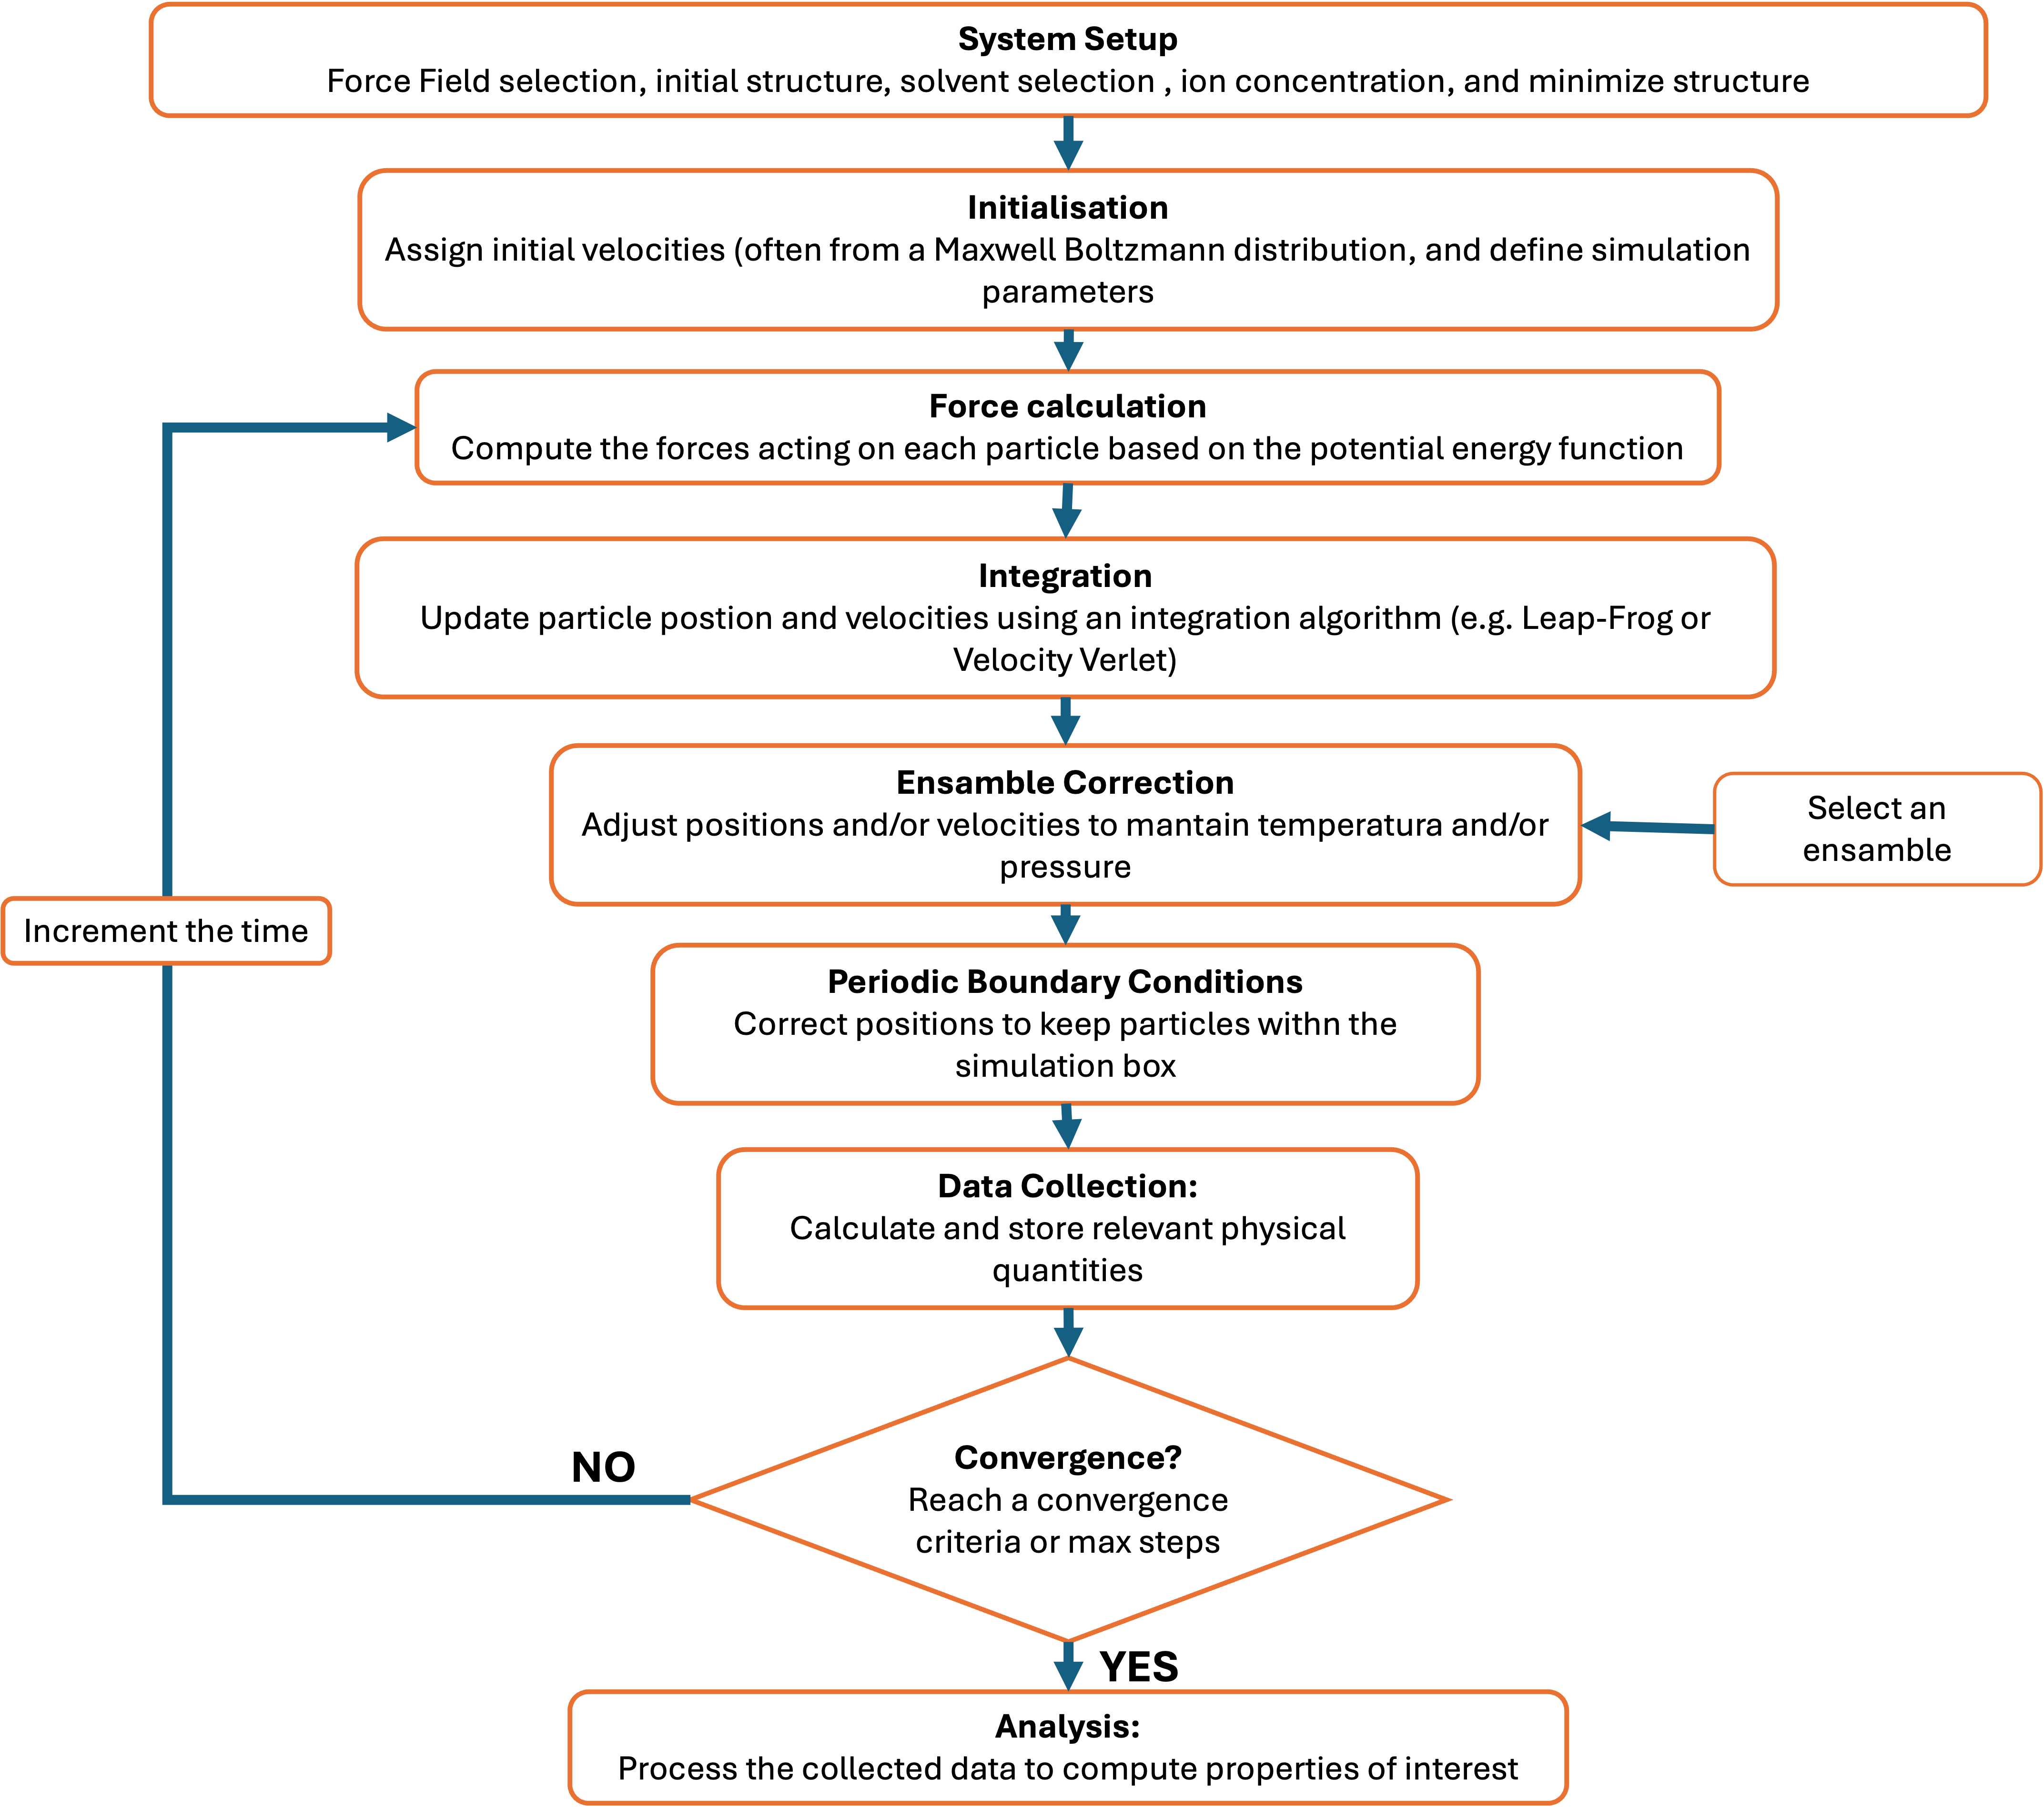
\includegraphics[width=1.0\linewidth]{General_Sections/Figures/MD_Workflow3.png}
    \caption{This scheme illustrates the essential steps involved in a MD simulation. The process begins with the definition of the initial state of the system, including the atomic coordinates and velocities, the selection of an appropriate force field, and the specification of the simulation conditions. The force field is then employed to compute the forces acting on each particle, which enables the time evolution of the system through the numerical integration of the equations of motion. At each time step, additional algorithms are applied to ensure that the system evolves under the desired thermodynamic conditions, such as constant temperature and/or pressure. This includes, for instance, the use of thermostats and barostats to control the corresponding ensemble. The propagation of positions and velocities, together with the enforcement of these conditions, is repeated iteratively over successive time steps. The simulation proceeds until a predefined convergence criterion is met or the maximum number of integration steps is reached.}
    \label{fig:MDFlow}
\end{figure}

The simulation process begins with system construction, including the selection of the force field, generation of the initial structure, solvent and ion setup, and energy minimization. Initial velocities are then assigned and simulation parameters are defined. At each time step, forces are computed from the potential energy function such as: 
\begin{equation}\label{NG}
    \vec{F_i} = - \vec{\nabla} U(\vec{r_{i}})
\end{equation}
Where $\vec{F}_i$ is the force acting on the $i$-th particle of the system, and $\vec{\nabla} U(\vec{r}_i)$ is the gradient of the potential energy function $U(\vec{r}_i)$, which is defined by a set of mathematical equations and parameters that collectively constitute a force field (FF). The selection of the FF is critical; it must faithfully reproduce the system's physical properties, as it governs the simulation's outcome~\cite{sereina,Conde2022}. Next, the position of the atoms are calculated by numerically integrating Newton's second law:
\begin{equation}\label{N2L}
    \vec{F}_i 
    = \frac{d\vec{p}_i}{dt}
    \xrightarrow{\text{constant }m_i}
    m_i \frac{d^2\vec{r}_i}{dt^2}
\end{equation}
where \(\vec{p}_i\), \(\vec{v}_i\) and \(m_i\) are the momentum, velocity, and mass of the \(i\)-th particle of the system, respectively, and \(t\) represents time. 
In a purely continuous and theoretical framework, the particle trajectory is
obtained by solving a second-order ordinary differential equation for the
position $\vec{r}_i(t)$, with time $t$ as the independent variable. Given an
initial position $\vec{r}_i(0)$ and velocity $\vec{v}_i(0)$, the state of the
system at any future time $t$ is determined by the solution of the equation
of motion:

\begin{equation}\label{eq:integral_v}
    \vec{v}_i(t) = \vec{v}_i(0) + \int_{0}^{t} \frac{\vec{F}_i(t')}{m_i} dt'
\end{equation}

\begin{equation}\label{eq:integral_r}
    \vec{r}_i(t) = \vec{r}_i(0) + \int_{0}^{t} \vec{v}_i(t') dt'
\end{equation}

However, because the force $\vec{F}_i$ acting on any single particle depends continuously on the ever-changing coordinates of all other interacting particles in the system, the integral in Equation~\ref{eq:integral_v} has no general analytical solution for a system of $N \geq 3$ particles. Consequently, evaluating the temporal evolution of the system requires shifting from a continuous analytical integration to a discrete numerical approximation.

This computational approach advances the simulation in finite, microscopic time increments, known as the time step ($\Delta t$). To achieve this, integration algorithms rely on the Taylor series expansion of the particle coordinates~\cite{braun2018best,biblia_2}. Mathematically, the Taylor series expansion of a general function $f(x)$ around a known point $a$ is expressed as:

\begin{equation}\label{eq:taylor_general}
    f(x) = f(a) + f'(a)(x-a) + \frac{f''(a)}{2!}(x-a)^2 + \frac{f'''(a)}{3!}(x-a)^3 + \dots
\end{equation}

By adapting this mathematical definition to the kinematics of a particle, the function becomes the position $\vec{r}_i$, the known point is the current time $t$, and the evaluated point is a small step forward in time ($t + \Delta t$). Consequently, the displacement $(x-a)$ corresponds to the time step $\Delta t$. Thus, the future position can be expanded as:

\begin{equation}\label{eq:taylor_forward}
    \vec{r}_i(t + \Delta t) = \vec{r}_i(t) + \vec{v}_i(t)\Delta t + \frac{1}{2}\vec{a}_i(t)\Delta t^2 + \frac{1}{6}\vec{j}_i(t)\Delta t^3 + \mathcal{O}(\Delta t^4)
\end{equation}
where $\vec{v}_i$ is the velocity (first derivative), $\vec{a}_i$ is the acceleration ($\vec{F}_i/m_i$, second derivative), $\vec{j}_i$ is the jerk (third derivative), and $\mathcal{O}(\Delta t^4)$ represents the local truncation error encompassing all higher-order terms. 

Similarly, to determine the position of the particle at the previous time step ($t - \Delta t$), we simply substitute $\Delta t$ with $-\Delta t$ in Equation~\ref{eq:taylor_forward}. Due to the alternating signs of the polynomial powers, this substitution yields:

\begin{equation}\label{eq:taylor_backward}
    \vec{r}_i(t - \Delta t) = \vec{r}_i(t) - \vec{v}_i(t)\Delta t + \frac{1}{2}\vec{a}_i(t)\Delta t^2 - \frac{1}{6}\vec{j}_i(t)\Delta t^3 + \mathcal{O}(\Delta t^4)
\end{equation}

By summing Equation~\ref{eq:taylor_forward} and Equation~\ref{eq:taylor_backward}, the odd-order derivatives (such as the velocity and the jerk) cancel out perfectly. Rearranging the result yields the classic Verlet integration algorithm~\cite{Verlet1967}:

\begin{equation}\label{eq:verlet}
    \vec{r}_i(t + \Delta t) = 2\vec{r}_i(t) - \vec{r}_i(t - \Delta t) + \frac{\vec{F}_i(t)}{m_i}\Delta t^2 + \mathcal{O}(\Delta t^4)
\end{equation}

Although the standard Verlet algorithm is computationally efficient and exhibits good numerical stability, it presents two important practical limitations. First, the position update involves the subtraction of two positions of similar magnitude, $2\vec{r}_i(t)-\vec{r}_i(t-\Delta t)$, which can lead to a loss of numerical precision due to floating-point round-off errors. Second, velocities do not explicitly enter the integration scheme and therefore must be estimated separately, typically from positions at adjacent time steps. This complicates the direct evaluation of the instantaneous kinetic energy and the application of temperature-control schemes based on the system's velocities.
To address these limitations, the \textit{leap-frog} integrator is widely used in molecular dynamics simulations and is the default integrator in the GROMACS simulation suite~\cite{leapfrog}. The leap-frog scheme is mathematically equivalent to the original Verlet algorithm, but reformulates the integration by evaluating velocities at half-integer time steps, $t\pm\frac{1}{2}\Delta t$, while positions are evaluated at integer time steps. The resulting staggered update of positions and velocities provides a more convenient representation of the system's dynamical state. The integration proceeds according to the following sequence:

\begin{equation}\label{eq:leapfrog}
    \begin{cases}
        \vec{v}_i(t+\frac{1}{2}\Delta t) = \vec{v}_i(t-\frac{1}{2}\Delta t) + \cfrac{\vec{F}_i(t)}{m_i} \Delta t \\
        \vec{r}_i(t+\Delta t) = \vec{r}_i(t) + \vec{v}_i(t+\frac{1}{2}\Delta t) \Delta t
    \end{cases}
\end{equation}
By structuring the integration in this staggered manner, the leap-frog scheme avoids the subtraction of large, closely spaced coordinate values present in the original Verlet formulation, thereby reducing the associated loss of numerical precision. At each time step, the forces acting on the particles are evaluated from the current configuration and used to update their velocities and positions. Repeated application of these equations generates the time evolution of the molecular system, providing the trajectory from which dynamical and thermodynamic properties can subsequently be calculated.

\paragraph{Constraint algorithms and the integration time step}

The selection of the integration time step is a critical factor governing the computational efficiency, numerical stability, and accuracy of MD simulations. Since the computational cost required to simulate a trajectory of a given physical duration increases as the time step decreases, using the largest stable $\Delta t$ is highly desirable~\cite{Conde2022}. However, the maximum allowable time step is constrained by the highest-frequency degrees of freedom in the system. To avoid numerical instability and limit integration errors, the time step must be sufficiently smaller than the period of the fastest internal motion, which typically corresponds to bond-stretching vibrations involving hydrogen atoms. Consequently, all-atom molecular systems without constraints typically require time steps of approximately 1~fs or smaller~\cite{Feenstra1999,Conde2022}.

To overcome this limitation and enable the use of larger integration time steps, constraint algorithms are routinely employed to remove selected high-frequency bond vibrations from the explicitly integrated degrees of freedom. In all-atom simulations, this commonly allows a time step of 2~fs to be employed. The SHAKE algorithm~\cite{shake_algorithm} was one of the earliest iterative methods developed to satisfy prescribed distance constraints. In modern GROMACS simulations, the parallel Linear Constraint Solver (LINCS) algorithm~\cite{lincs_algorithm} is widely used because of its computational efficiency and suitability for parallel implementations. Rather than iteratively solving the constrained equations of motion, LINCS determines the required corrections through a matrix-based linear constraint formulation. Additionally, because water molecules constitute a substantial fraction of the particles in biological systems, the analytical SETTLE algorithm~\cite{settle_algorithm} is specifically designed to enforce the rigid geometry of common water models, providing an efficient treatment of water constraints.

In the absence of external coupling, the underlying Newtonian equations of motion conserve the total energy of an isolated system. For a system with a fixed number of particles ($N$) and volume ($V$), the resulting dynamics therefore correspond to the microcanonical (\textit{NVE}) ensemble. In practice, however, numerical integration introduces small deviations from exact energy conservation, whose magnitude depends on the integration scheme and time step. Nevertheless, most biological processes in nature and experiments in the laboratory occur under approximately constant temperature ($T$) and/or pressure ($P$). Consequently, biomolecular simulations are frequently performed in the canonical (\textit{NVT}) or isothermal-isobaric (\textit{NPT}) ensembles~\cite{Frenkel2023,schlick2010molecular}. To reproduce these thermodynamic conditions, additional algorithms are introduced to couple the system to thermal and/or pressure reservoirs. Algorithms that regulate pressure are referred to as \textit{barostats}. They modify the dimensions and, consequently, the volume of the simulation cell according to the instantaneous pressure and the desired reference pressure. Several barostats are available for this purpose, including the stochastic cell-rescaling approach~\cite{CRB}. However, in the present work, only the Berendsen~\cite{BerendsenB} and Parrinello--Rahman~\cite{Parrinello1981} barostats were employed sequentially during equilibration and production simulations.

Similarly, algorithms that regulate temperature are referred to as \textit{thermostats}. These methods modify the kinetic degrees of freedom of the system to control its temperature. Depending on the algorithm, temperature regulation can be achieved through different mechanisms, including coupling the system to an external thermal bath or directly modifying the particle velocities. The latter principle underlies the velocity-rescaling thermostat employed in the present work~\cite{Vresc}.











































\subsection{Thermostats and barostats}

\paragraph{Statistical mechanics of temperature control}

According to the equipartition theorem, each degree of freedom contributes $k_B T / 2$ to the total energy, yielding the kinetic energy; $K = \frac{N_f}{2} k_B T$, where $N_f$ is the number of degrees of freedom and $k_B$ is the Boltzmann constant~\cite{nolting2018theoretical}. However, in a real system coupled to a thermal bath, the instantaneous kinetic energy is not strictly constant; it fluctuates. 

To determine the exact probability distribution of these macroscopic fluctuations, $P(K)$, we must first examine the system at the microscopic level. In the canonical (\textit{NVT}) ensemble, the probability of finding the system in one specific, exact microscopic state; defined by a unique set of individual momentum vectors $\{\vec{p}_i\}$; is governed strictly by the Boltzmann factor:

\begin{equation}
    P(\vec{p}_1, \vec{p}_2, \dots, \vec{p}_N) \propto e^{-K / k_B T_{\text{ref}}}
\end{equation}

However, in a macroscopic MD simulation, there are countless different ways to distribute the individual momenta among the particles that result in the exact same total $K$. To find the total probability of observing a macroscopic energy $K$, we must multiply the probability of a single microstate by the density of states, $\Omega(K)$~\cite{termo_metad_presion}. This crucial thermodynamic term quantifies the degeneracy of the system, representing the total number of microscopic momentum combinations that yield that exact total energy $K$:

\begin{equation}
    P(K) = \Omega(K) e^{-K / k_B T_{\text{ref}}}
\end{equation}

To mathematically determine this density of states $\Omega(K)$, we can use a geometric approach in phase space. Assuming for simplicity that all particles have the same mass $m$, the kinetic energy equation can be rewritten as $\sum_{i=1}^{N_f} p_i^2 = 2mK$, where $p_i$ represents each individual scalar momentum component. Mathematically, this equation perfectly matches the definition of the surface of an $N_f$-dimensional hypersphere, whose radius is $R = \sqrt{2mK} \propto K^{1/2}$. 

Geometrically, the surface area of such a hypersphere, and thus the number of available microstates $\Omega(K)$, scales as the radius raised to the power of the dimensions minus one ($R^{N_f - 1}$). Therefore, the density of states is proportional to~\cite{mec_estadistica}:

\begin{equation}
    \Omega(K) \propto (K^{1/2})^{N_f - 1} = K^{(N_f - 1)/2}
\end{equation}

 To express the final probability $P(K)$ in terms of the kinetic energy rather than momentum, a change of variables is required. Since $K \propto p^2$, the differentials relate as $dK \propto p\,dp$, which yields $dp \propto K^{-1/2} dK$. Combining the geometrical density of states with this differential change yields the final statistical weight:

\begin{equation}
    \Omega(K) \, dp \propto K^{(N_f - 1)/2} K^{-1/2} = K^{N_f/2 - 1}
\end{equation}

By incorporating this term into the macroscopic probability equation, the exact theoretical distribution of the kinetic energy in the \textit{NVT} ensemble is obtained as a Gamma distribution~\cite{gamma}:

\begin{equation}\label{eq:gamma_distribution}
    P(K) \propto K^{N_f/2 - 1} e^{-K / k_B T_{\text{ref}}}
\end{equation}

 By direct comparison\footnote{In probability theory, a Gamma distribution defined by a random variable $x$, a shape parameter $k$, and a scale parameter $\theta$ follows the proportionality $f(x) \propto x^{k-1} e^{-x/\theta}$.}, $K$ is the random variable, with shape parameter $k = N_f/2$ and scale parameter $\theta = k_B T_{\text{ref}}$. Its variance is therefore $\mathrm{Var}(K) = \frac{N_f}{2}(k_B T_{\text{ref}})^2$, which statistical mechanics dictates must be reproduced by any valid \textit{NVT} ensemble:

\begin{equation}\label{eq:variance_k}
    \sigma_K^2 = \langle K^2 \rangle - \langle K \rangle^2 = \frac{N_f}{2} (k_B T_{\text{ref}})^2
\end{equation}

Computationally, MD engines integrate Newton's equations of motion. In the absence of external coupling, these equations describe dynamics at constant total energy, corresponding to the microcanonical ($NVE$) ensemble, rather than the canonical ($NVT$) ensemble, in which the system exchanges energy with a thermal reservoir at a prescribed temperature. Thermostats introduce this coupling by modifying the particle dynamics to regulate the kinetic energy and thereby control the temperature. For velocity-rescaling thermostats, this is achieved through a scaling factor $\alpha$ applied to the particle velocities, while other thermostat families modify the equations of motion through different extended-system or stochastic formulations~\cite{BerendsenB,Vresc}. The physical behavior of rescaling-based thermostats therefore depends on how this scaling factor is determined.
The most rudimentary temperature-control scheme, known as \emph{simple velocity rescaling}, bypasses the natural thermodynamic fluctuations entirely. At each integration step, it forces the system to the exact target temperature by applying a rigid scaling factor defined as $\alpha = \sqrt{T_{\text{ref}}/T}$. 

To understand why this procedure is physically problematic, consider how this scaling factor affects the total kinetic energy. If every particle velocity is scaled according to $\vec{v}_i^{,\mathrm{new}} = \alpha \vec{v}_i$, the new total kinetic energy becomes:

\begin{equation}
K_{\mathrm{new}}
= \sum_{i=1}^{N} \frac{m_i(\alpha\vec{v}_i)\cdot(\alpha\vec{v}_i)}{2}
= \alpha^2 \sum_{i=1}^{N} \frac{m_i(\vec{v}_i\cdot\vec{v}_i)}{2}
= \alpha^2 K
\end{equation}
Substituting $\alpha^2 = T_{\mathrm{ref}}/T$ and using the proportionality between temperature and kinetic energy, $T_{\mathrm{ref}}/T = K_{\mathrm{ref}}/K$, gives:
\begin{equation}
K_{\mathrm{new}}
= \left(\frac{K_{\mathrm{ref}}}{K}\right)K
= K_{\mathrm{ref}}
\end{equation}
Thus, the instantaneous kinetic energy is forced to be identically equal to the target value at the end of every integration step. Consequently, its variance in the simulated system is zero, $\sigma_K^2=0$. A distribution with a fixed value and zero variance collapses mathematically to a Dirac delta function,
\begin{equation}
P_{\mathrm{simulated}}(K)
= \delta(K-K_{\mathrm{ref}})
\end{equation}
Simple velocity rescaling therefore imposes an isokinetic constraint rather than sampling the canonical ($NVT$) ensemble, eliminating the kinetic-energy fluctuations required for canonical sampling.


\paragraph{The Berendsen thermostat}

To avoid the unphysical abruptness of simple velocity rescaling, the
Berendsen thermostat introduces a gradual relaxation of the system towards
the target temperature over a specified relaxation time, $t_r$~\cite{BerendsenB}.
Since temperature is proportional to the instantaneous kinetic energy, this
relaxation can equivalently be expressed in terms of the kinetic energy $K$
as a first-order deterministic differential equation:

\begin{equation}\label{eq:berendsen_dk}
    \frac{dK}{dt}
    =
    \frac{K_{\mathrm{ref}}-K}{t_r}
\end{equation}

For a discrete integration time step $\Delta t$, the change in kinetic
energy is:

\begin{equation}
    \Delta K
    =
    (K_{\mathrm{ref}}-K)
    \frac{\Delta t}{t_r}
\end{equation}

Since the new kinetic energy is:

\begin{equation}
    K_{\mathrm{new}} = K + \Delta K
\end{equation}

and rescaling all particle velocities by a factor $\alpha$ changes the
kinetic energy according to:

\begin{equation}
    K_{\mathrm{new}} = \alpha^2 K
\end{equation}

the scaling factor can be obtained as:

\begin{equation}
    \alpha^2 K
    =
    K+
    (K_{\mathrm{ref}}-K)\frac{\Delta t}{t_r}
\end{equation}

which gives:

\begin{equation}
    \alpha
    =
    \sqrt{
        1+
        \frac{\Delta t}{t_r}
        \left(
            \frac{K_{\mathrm{ref}}}{K}-1
        \right)
    }
\end{equation}

Because the kinetic energy is proportional to the instantaneous temperature,
$K \propto T$, this expression can equivalently be written as:

\begin{equation}
    \alpha
    =
    \sqrt{
        1+
        \frac{\Delta t}{t_r}
        \left(
            \frac{T_{\mathrm{ref}}}{T}-1
        \right)
    }
\end{equation}

\paragraph{The stochastic v-rescale solution}

To circumvent the limitations of both simple rescaling (zero variance) and Berendsen (artificially restricted variance), Bussi, Donadio, and Parrinello introduced the stochastic velocity-rescaling algorithm (\textit{v-rescale})~\cite{Vresc}. Their crucial insight was to supplement the deterministic relaxation of the kinetic energy used in the Berendsen approach with an explicit stochastic contribution.
They redefined the evolution of the kinetic energy using a stochastic differential equation:


\begin{equation}\label{eq:vrescale}
    dK = \underbrace{(K_{\text{ref}} - K)\frac{dt}{t_r}}_{\text{Deterministic relaxation}} + \underbrace{2\sqrt{\frac{K K_{\text{ref}}}{N_f t_r}} dW}_{\text{Stochastic thermal noise}}
\end{equation}

The first term represents the deterministic relaxation of the kinetic energy towards its target value, analogous to the Berendsen thermostat. The second term introduces stochastic fluctuations through a Wiener process $dW$. The amplitude of this stochastic contribution is chosen such that, under the corresponding Fokker--Planck equation, the stationary distribution of the kinetic energy is the canonical Gamma distribution~\cite{Vresc}.

Consequently, the \textit{v-rescale} algorithm derives a stochastic scaling factor that ensures the stationary probability distribution of the kinetic energy converges to the theoretical Gamma distribution (Equation~\ref{eq:gamma_distribution}). This preserves the stable temperature relaxation of the Berendsen approach while correctly reproducing the thermodynamic fluctuations required to sample the canonical ($NVT$) ensemble~\cite{Vresc}.















\subsubsection{Statistical mechanics of pressure control}

To understand how barostats operate, it is first necessary to define how pressure is calculated at the microscopic level. In molecular simulations using Periodic Boundary Conditions (PBCs), there are no physical walls against which particles exert force. Instead, the instantaneous pressure is calculated from the microscopic virial expression. Because interactions can contribute differently along the three spatial directions ($X$, $Y$, and $Z$), pressure is generally represented by a $3\times3$ pressure tensor, $\mathbf{P}$, which contains kinetic and virial contributions~\cite{termo_metad_presion}:

\begin{equation}\label{eq:virial_tensor}
    \mathbf{P} = \frac{1}{V} \left( \underbrace{\sum_{i=1}^{N} \frac{\vec{p}_i \otimes \vec{p}_i}{m_i}}_{\text{Kinetic contribution}} - \underbrace{\sum_{i=1}^{N-1} \sum_{j=i+1}^{N} \vec{r}_{ij} \otimes \vec{f}_{ij}}_{\text{Virial contribution}} \right)
\end{equation}
where $V$ is the volume of the simulation cell, $\vec{p}_i$ is the momentum vector of particle $i$, $\vec{r}_{ij}$ is the displacement vector between two interacting particles, and $\vec{f}_{ij}$ is the force vector acting between them. The symbol $\otimes$ denotes the 
outer product of two vectors, yielding a second-order $3 \times 3$ tensor; explicitly, $(\vec{a} \otimes \vec{b})_{ij} = a_i b_j$. For an isotropic system, the scalar pressure is obtained as one-third of the trace of the pressure tensor: $p = \text{Tr}(\mathbf{P})/3$.

In an $NVT$ simulation, the volume is fixed, while the instantaneous pressure fluctuates as the particles move. In an $NPT$ simulation, the volume of the simulation cell is allowed to fluctuate around a value consistent with a prescribed reference pressure, $\mathbf{P}_{\mathrm{ref}}$. Depending on the pressure-coupling scheme, the shape of the simulation cell may also be allowed to fluctuate. In pressure-coupling schemes based on cell rescaling, pressure deviations are compensated by applying a scaling transformation to the simulation cell and the particle coordinates. A general rescaling can be represented by a transformation matrix $\mathbf{M}$ acting on the particle coordinates and the simulation-cell volume:

\begin{subequations}\label{eq:scaling_general}
    \begin{align}
        \vec{x} &\rightarrow \mathbf{M}\vec{x} \\
        V &\rightarrow \det(\mathbf{M})V
    \end{align}
\end{subequations}

Here, $\mathbf{M}$ determines the deformation applied to the simulation cell, including changes in its dimensions and, for anisotropic coupling, its shape. The specific form of this transformation depends on the pressure-coupling scheme.


\paragraph{The Berendsen barostat}
The Berendsen barostat provides a simple and stable procedure for relaxing the simulation box towards a prescribed reference pressure~\cite{BerendsenB}. Its underlying principle is that deviations between the instantaneous pressure and the reference pressure induce a gradual change in the dimensions of the simulation box. The magnitude of this response depends on the pressure difference, the isothermal compressibility of the system, and the chosen pressure-relaxation time $t_r$.
For the Berendsen scheme, the scaling matrix can be written as:
\begin{equation}\label{eq:berendsen}
\mathbf{M}
=
\mathbb{I}
-
\frac{\Delta t}{3t_r}
\boldsymbol{\beta}
\odot
\left(
\mathbf{P}
-
\mathbf{P}_{\mathrm{ref}}
\right)
\end{equation}
where $\Delta t$ is the integration timestep, $\boldsymbol{\beta}$ is the isothermal compressibility tensor, and $\odot$ denotes the Hadamard
(element-wise) product. Here, $\mathbb{I}$ represents the identity transformation, while the pressure difference
$\mathbf{P}-\mathbf{P}_{\mathrm{ref}}$ determines the magnitude of the box deformation, with different components contributing independently in anisotropic coupling. The compressibility determines the response of the system to a pressure difference, while the relaxation time
$t_r$ controls the rate of the response.

For isotropic pressure coupling, a common scaling factor is applied to the three spatial dimensions. In anisotropic or semi-isotropic coupling, the corresponding components of the pressure and compressibility tensors determine how the individual box dimensions are scaled. The scaling is therefore applied gradually over successive integration steps rather than enforcing an instantaneous pressure correction.
An important limitation of the Berendsen barostat is that the deterministic rescaling suppresses the magnitude of the natural fluctuations of the simulation cell. Consequently, although it provides efficient pressure relaxation, it does not generate the correct volume fluctuations of the isothermal-isobaric ensemble~\cite{BerendsenB}.

\paragraph{The stochastic cell-rescaling (C-rescale) barostat}
The stochastic cell-rescaling (C-rescale) barostat is a stochastic variant of the Berendsen pressure-coupling scheme that allows the correct equilibrium volume fluctuations to be sampled~\cite{CRB}. As in the Berendsen approach, the simulation coordinates and box vectors are rescaled at regular intervals, producing a first-order relaxation of the pressure towards a prescribed reference pressure. The difference is that the rescaling includes a stochastic contribution that restores the equilibrium volume fluctuations.
For isotropic pressure coupling, the volume evolution can be expressed in terms of the volumetric strain $\epsilon=\log(V/V_0)$ as~\cite{CRB,Gromacs2015}:
\begin{equation}\label{eq:crescale}
d\epsilon
=
-\frac{\beta}{t_r}
\left(
P_{\mathrm{ref}}-P
\right)dt
+
\sqrt{
\frac{2k_BT\beta}{Vt_r}
}\,dW
\end{equation}
where $\beta$ is the isothermal compressibility, $t_r$ is the pressure-relaxation time, $V$ is the instantaneous simulation-cell volume, and $dW$ represents an increment of a Wiener process. The first term describes the deterministic relaxation of the pressure towards the reference pressure, analogous to the Berendsen scheme, whereas the second term introduces stochastic fluctuations into the cell-rescaling process.
Unlike the deterministic Berendsen barostat, the stochastic contribution allows C-rescale to reproduce the correct equilibrium volume fluctuations of the $NPT$ ensemble while retaining a first-order pressure-relaxation behavior~\cite{CRB}.

\paragraph{The Parrinello--Rahman barostat}
The Parrinello--Rahman approach differs fundamentally from direct cell-rescaling methods because the simulation cell itself is treated as a set of additional dynamical degrees of freedom~\cite{Parrinello1981}. Rather than prescribing an instantaneous scaling factor, the method introduces an extended Lagrangian in which the cell vectors evolve dynamically in response to the difference between the instantaneous and reference pressure tensors.
Let $\mathbf{L}$ denote the cell matrix, whose columns are the three vectors defining the simulation cell. In the Parrinello--Rahman formulation, the cell dynamics can be written schematically as:
\begin{equation}\label{eq:parrinellorahman1}
\ddot{\mathbf{L}}
=
V\mathbf{W}^{-1}
\left(\mathbf{L}^{\mathrm{T}}\right)^{-1}
\left(
\mathbf{P}
-
\mathbf{P}_{\mathrm{ref}}
\right)
\end{equation}
where $V$ is the simulation-cell volume and $\mathbf{W}$ is a matrix parameter that controls the inertial response of the simulation cell~\cite{Gromacs2015}. Thus, deviations between the instantaneous and reference pressure tensors drive the dynamical deformation of the simulation cell.
Because the simulation cell evolves dynamically, its deformation is also coupled to the particle motion. Consequently, the equations of motion are modified to account for the time-dependent geometry of the simulation cell. By treating the simulation cell as a dynamical degree of freedom, the Parrinello--Rahman method allows the system to reproduce the correct equilibrium fluctuations of the isothermal-isobaric ($NPT$) ensemble.
However, the dynamical response of the cell can lead to pronounced oscillations when the system is far from the target pressure. Therefore, Parrinello--Rahman coupling is generally more appropriate after an initial equilibration stage, when the pressure and volume are already reasonably close to their target values.




\paragraph{Comparison and application of pressure coupling methods}

The three barostats considered here differ in their treatment of pressure relaxation and volume fluctuations, making them suitable for different stages of an MD simulation. The Berendsen barostat provides stable and rapid relaxation towards the target pressure, which makes it useful during the initial equilibration of the system. However, because it suppresses the natural pressure and volume fluctuations, it does not sample the correct $NPT$ ensemble. In contrast, the Parrinello--Rahman barostat allows the system to sample the appropriate equilibrium fluctuations, but can exhibit substantial box oscillations when applied to systems that are far from mechanical equilibrium. It is therefore generally more suitable after an initial equilibration stage. The stochastic cell-rescaling (C-rescale) barostat combines pressure relaxation with stochastic fluctuations, allowing the correct equilibrium volume fluctuations to be reproduced while maintaining stable pressure relaxation~\cite{Gromacs2015,CRB}.
In the MD simulations presented in this thesis, the Berendsen barostat was therefore employed during the initial equilibration stages to allow the system volume to relax smoothly towards the target pressure, followed by Parrinello--Rahman during the production simulations to obtain the appropriate thermodynamic fluctuations.




\paragraph{Semi-isotropic pressure coupling: Preserving membrane integrity}
Lipid bilayers are mechanically anisotropic systems, with their response to pressure differing substantially between the membrane plane and the direction normal to it. Consequently, pressure coupling in membrane simulations requires the lateral ($XY$) and normal ($Z$) dimensions of the simulation box to be treated differently.
Under isotropic pressure coupling, the three box dimensions are coupled to the same pressure response. Such scaling is appropriate for approximately isotropic systems, but is generally not suitable for lipid bilayers because the membrane exhibits different mechanical responses in the lateral and normal directions. In contrast, semi-isotropic pressure coupling couples the two lateral dimensions, $X$ and $Y$, while treating them independently from the normal dimension, $Z$.
Thus, the lateral dimensions are scaled together to preserve the symmetry of the membrane plane, whereas the normal dimension is allowed to respond independently to the pressure along the membrane normal. This can be represented by a compressibility tensor of the form:
\begin{equation}
\begin{pmatrix}
\beta_{xy} & 0 & 0 \\
0 & \beta_{xy} & 0 \\
0 & 0 & \beta_z
\end{pmatrix}
\end{equation}
where $\beta_{xy}$ describes the common compressibility applied to the two lateral directions, while $\beta_z$ describes the response along the membrane normal.
This separation allows the membrane area to equilibrate independently from the box dimension normal to the bilayer, providing an appropriate treatment of the distinct lateral and normal responses of the membrane. The choice of pressure-coupling scheme can influence the structural and dynamical properties of lipid bilayers and should therefore be considered carefully in membrane simulations~\cite{Ivanova2018,Gromacs2015,10.1371/journal.pcbi.1000810}























































\subsection{Periodic boundary conditions}
Nevertheless, despite the thermodynamic control offered by these algorithms, the simulation of real-world systems is limited by the amount of particles that can be simulated using a realistic amount of computational resources. This limitation necessitates confining the molecules to a finite volume; however, enclosing them with hard boundaries would introduce artificial particle-wall interactions that are unrealistic for biological environments. To avoid this, when the calculation of the new positions displaces a particle out of the simulation cell, the exact same particle wraps around and re-enters from the opposite side.

This approach effectively models an infinite system by tiling the simulation cell in all directions of space, creating periodic replicas where every particle is and behaves exactly like its original counterpart. This method is depicted in Figure~\ref{fig:PBCs}, and when applied, the system is said to be under PBCs. When applying this method, the simulation box must be large enough to avoid any possible interactions between replicas of the same molecule~\cite{braun2018best}.
\begin{figure}[!htbp]
    \centering
    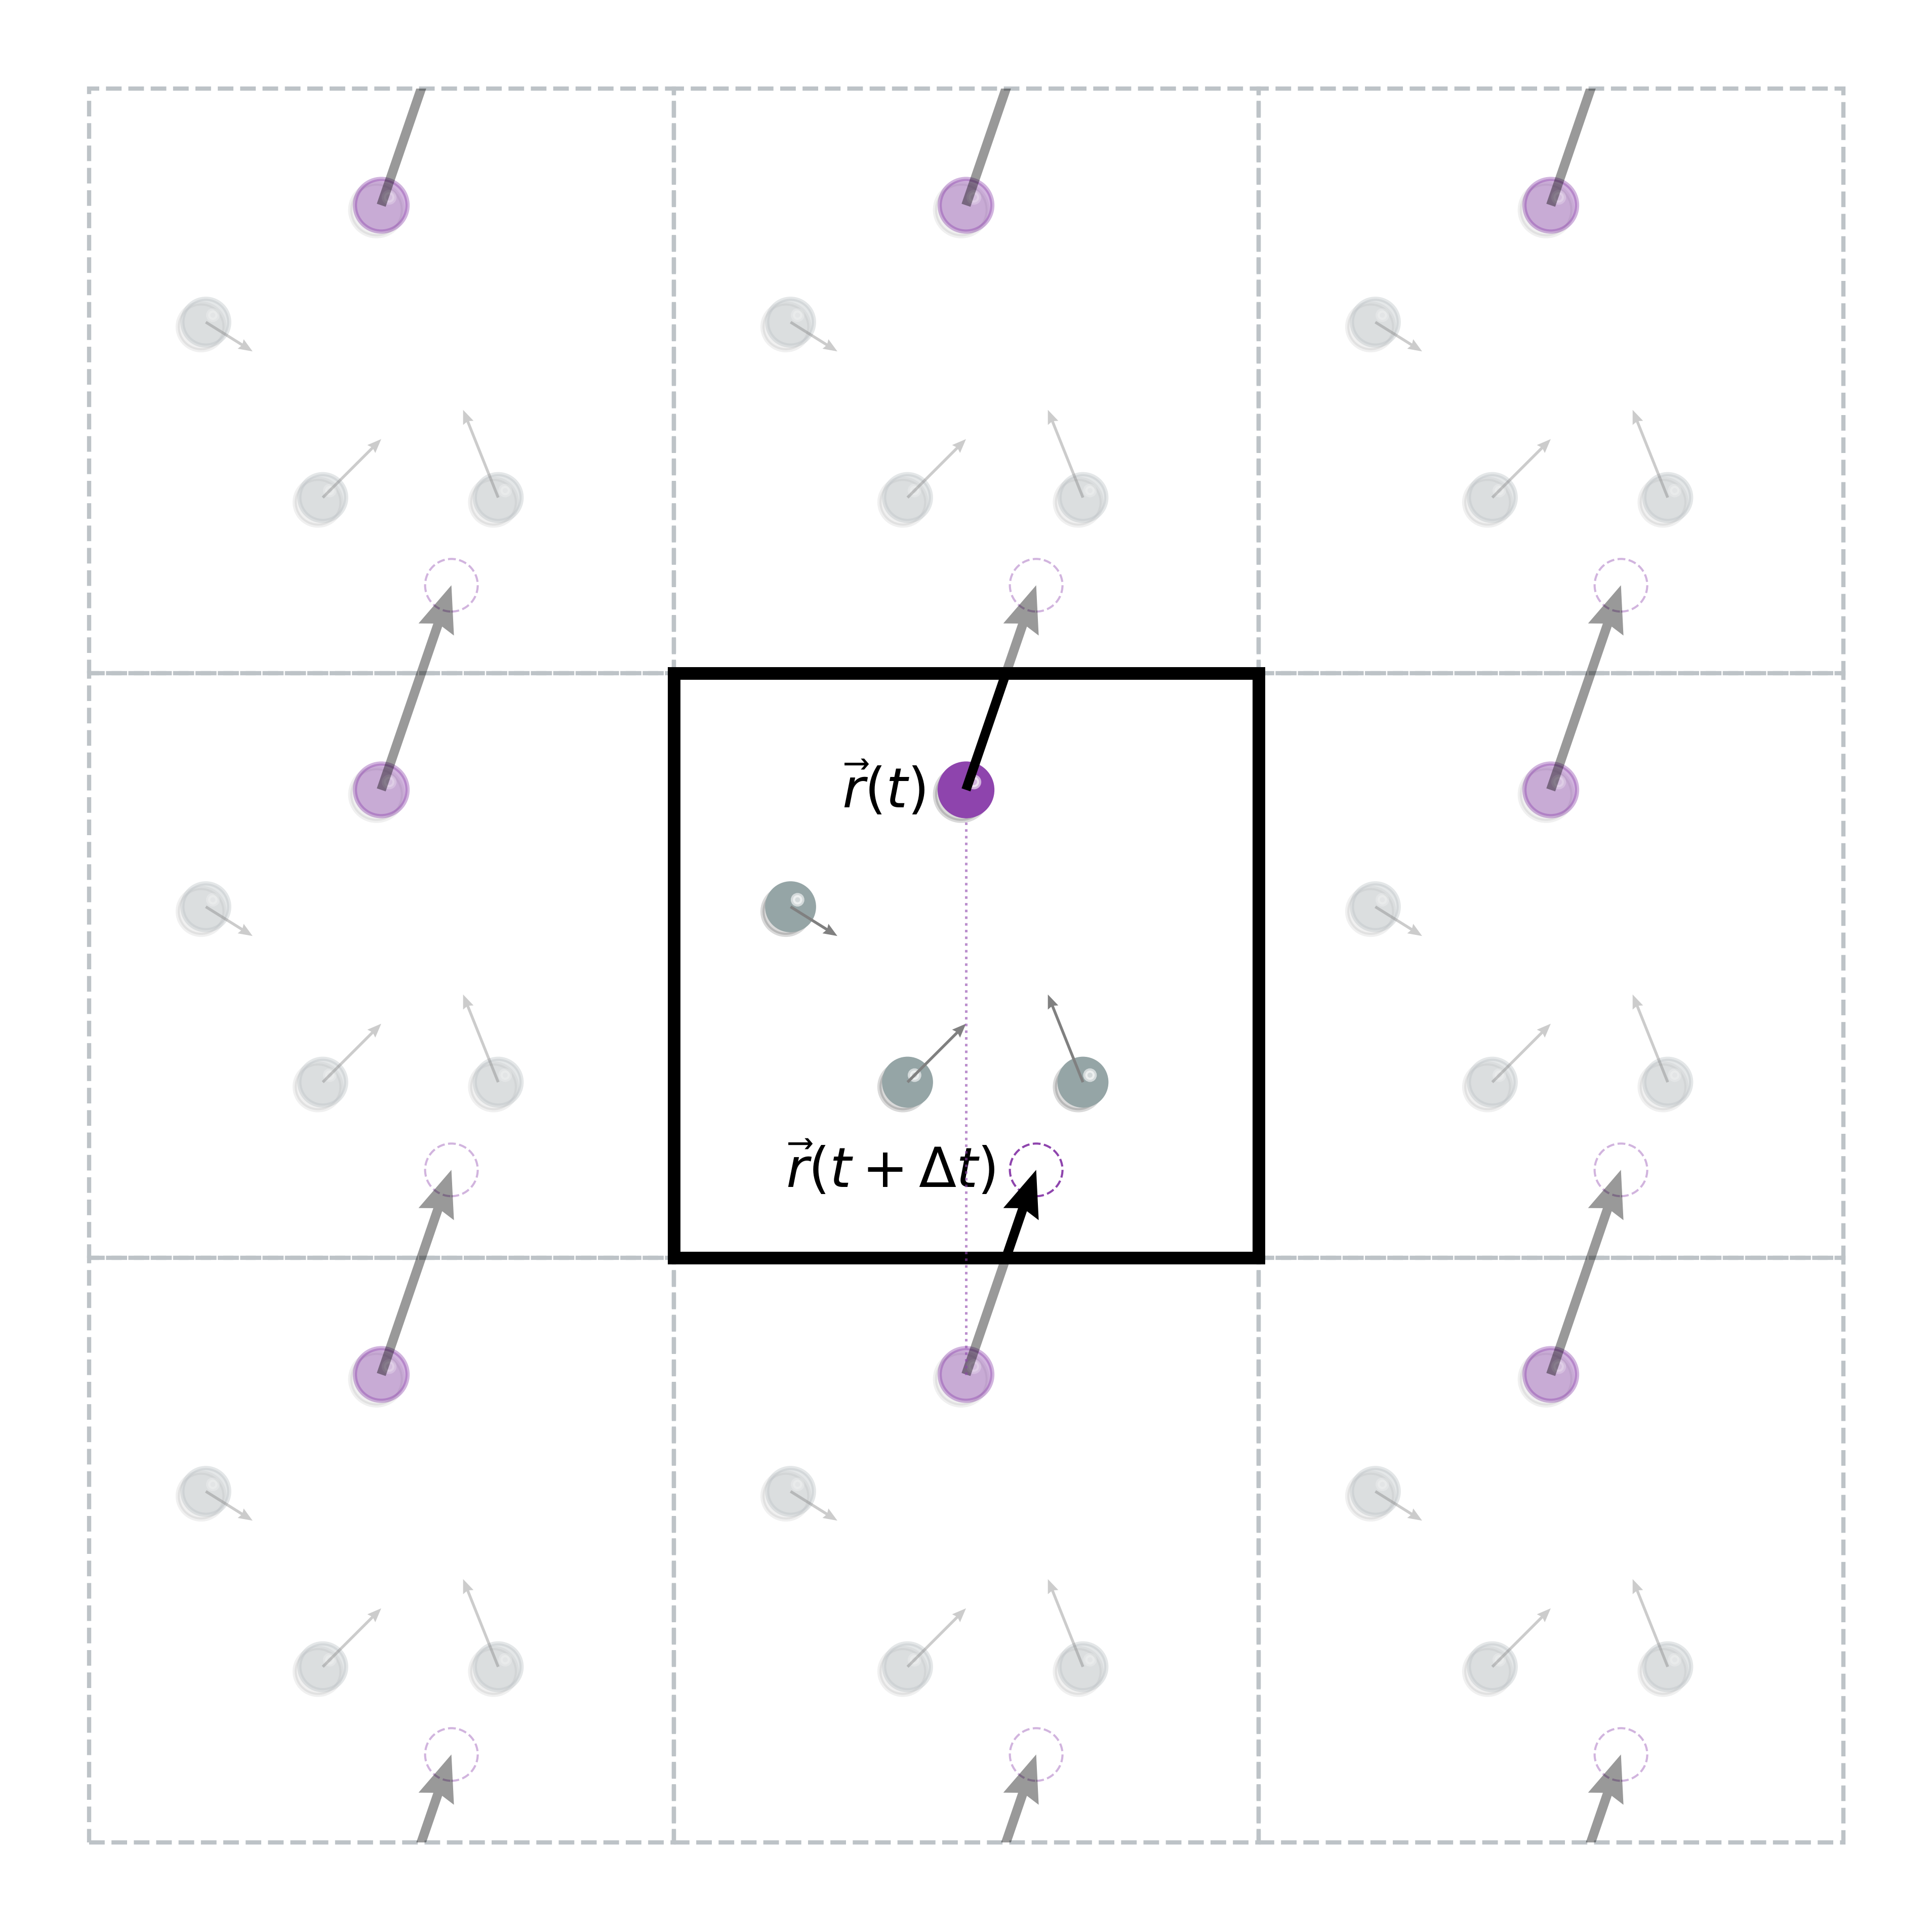
\includegraphics[width=0.55\linewidth]{General_Sections/Figures/pbc_diagram.png}
    \caption{Scheme depicting the effect of PBCs. The image shows how a particle that at an instant \(t\) is displaced outside the original simulation space (black solid line), re-enters into the box from its periodic image at a time \(t + \Delta t\). The number of particles in the simulation cell and in all the periodic images are kept constant. Image generated with Matplotlib.}
    \label{fig:PBCs}
\end{figure}
In the final step of the MD workflow shown in Figure~\ref{fig:MDFlow}, the MD engine writes the new positions, velocities, thermodynamic properties, and other relevant data into output files. If a convergence criterion is met or a user-defined number of steps are completed, the simulation finishes, allowing for subsequent qualitative and quantitative analysis. As noted above, the results obtained depend on the force field selected, as it governs the interactions between particles. The following section examines the general structure of force fields, with particular emphasis on the different contributions to the potential function used to compute the forces acting on each particle.


\subsection{Force fields}

A force field is a set of equations and parameters used to describe the potential energy of a molecular system and, consequently, the interactions between its particles. In general, the potential energy function can be decomposed into bonded and non-bonded contributions:

\begin{equation}
U(\vec{r}) =
U_{\mathrm{bonded}}(\vec{r}) +
U_{\mathrm{non-bonded}}(\vec{r})
\end{equation}

\subsubsection{Bonded interactions}
The bonded term describes interactions between particles whose relative positions are constrained by the molecular connectivity of the system. These interactions are defined by the covalent topology and account for local structural degrees of freedom, including bond stretching, angle bending, and torsional motions. The bonded contribution to the potential energy can be decomposed as:
\begin{equation}
U_{\mathrm{bonded}}(\vec{r}) =
U_{\mathrm{bonds}}(\vec{r}) +
U_{\mathrm{angles}}(\vec{r}) +
U_{\mathrm{proper\ dihedrals}}(\vec{r}) +
U_{\mathrm{improper\ dihedrals}}(\vec{r})
\end{equation}



The bond-stretching contribution describes the variation in distance between two covalently connected particles (Fig.~\ref{fig:bond_stretching}), whereas the angle-bending contribution accounts for variations in the angle formed by three consecutively connected particles (Fig.~\ref{fig:angle_bending}). Torsional contributions involve four particles and describe rotations about the corresponding molecular bonds. These are commonly divided into proper dihedrals, which describe torsion around a sequence of four consecutively connected particles (Fig.~\ref{fig:dihedral_proper}), and improper dihedrals, which constrain the relative geometry of four particles and are commonly used to maintain planarity or stereochemical configurations (Fig.~\ref{fig:dihedral_improper}).
\begin{figure}[!htb]
\centering

\begin{subfigure}[b]{0.48\linewidth}
    \centering
    
\includegraphics[width=0.95\linewidth]{bonded_interactions/bond_stretching.pdf}
    \caption{Bond stretching}
    \label{fig:bond_stretching}
\end{subfigure}
\hfill
\begin{subfigure}[b]{0.48\linewidth}
    \centering
    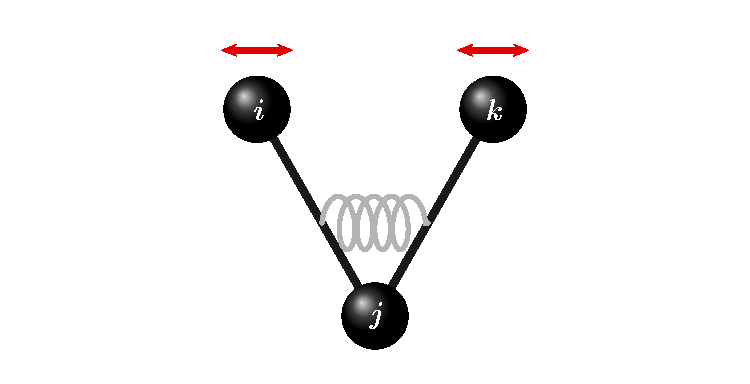
\includegraphics[width=0.95\linewidth]{bonded_interactions/angle_bending.pdf}
    \caption{Angle bending}
    \label{fig:angle_bending}
\end{subfigure}

\vspace{2ex}

\begin{subfigure}[b]{0.48\linewidth}
    \centering
    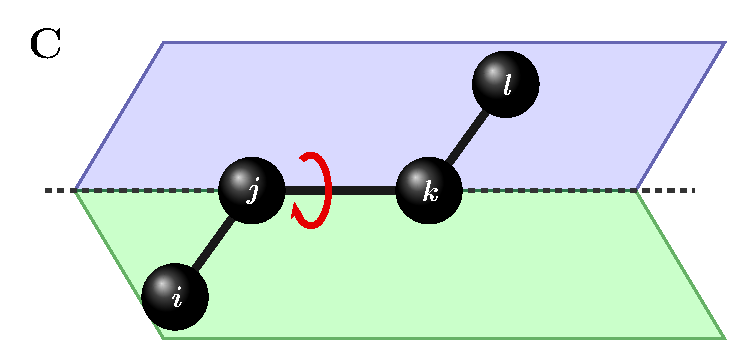
\includegraphics[width=0.95\linewidth]{bonded_interactions/dihedral_proper.pdf}
    \caption{Proper dihedral}
    \label{fig:dihedral_proper}
\end{subfigure}
\hfill
\begin{subfigure}[b]{0.48\linewidth}
    \centering
    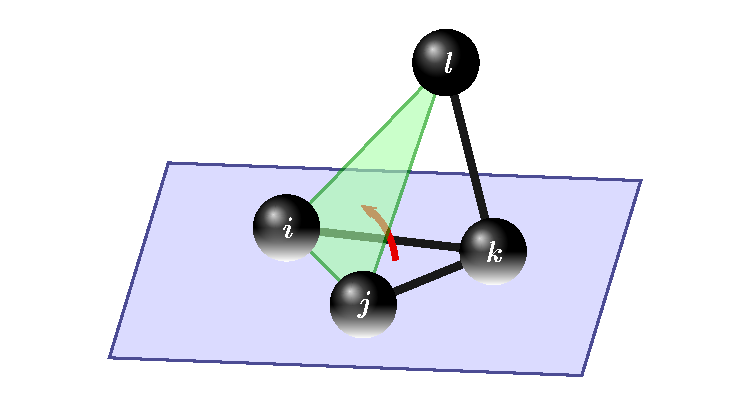
\includegraphics[width=0.95\linewidth]{bonded_interactions/dihedral_improper.pdf}
    \caption{Improper dihedral}
    \label{fig:dihedral_improper}
\end{subfigure}

\caption{Schematic representation of the bonded interactions included in the bonded term of the potential function. (a) Bond stretching between two covalently connected particles, (b) angle bending involving three consecutively connected particles, (c) torsion about a proper dihedral angle involving four consecutively connected particles, and (d) an improper dihedral used to control the relative arrangement of four particles.}
\label{fig:FF_bonded}

\end{figure}
Bond and angle terms are commonly represented using harmonic potentials:
\begin{equation}
U_{\mathrm{bonds}}(\vec{r}_{ij}) =
\frac{1}{2} k_{ij}
\left(
\vec{||r_{ij}||} - r_{ij}^{0}
\right)^2
\end{equation}

\begin{equation}
U_{\mathrm{angles}}(\theta_{ijk}) =
\frac{1}{2} k_{ijk}
\left(
\theta_{ijk} - \theta_{ijk}^{0}
\right)^2.
\label{eq:angle}
\end{equation}

Here, $\vec{r}_{ij}$ denotes the instantaneous distance between particles $i$ and $j$, whereas $r_{ij}^{0}$ is the corresponding equilibrium bond distance and $k_{ij}$ is the associated force constant. Similarly, $\theta_{ijk}$ is the instantaneous angle formed by particles $i$, $j$, and $k$, $\theta_{ijk}^{0}$ is its equilibrium value, and $k_{ijk}$ is the corresponding force constant. The values of these equilibrium geometries and force constants are determined by the specific force field and molecular topology.

The torsional contribution accounts for the rotational degrees of freedom associated with four connected particles. A common functional form for proper dihedrals is a periodic potential,
\begin{equation}
U_{\mathrm{proper\ dihedral}}(\phi_{ijkl}) =
k_{ijkl}
\left[
1 + \cos
\left(
n\phi_{ijkl} - \phi_{ijkl}^{0}
\right)
\right]
\end{equation}
where $\phi_{ijkl}$ is the instantaneous dihedral angle defined by particles $i$, $j$, $k$, and $l$, $n$ is the periodicity or multiplicity of the torsional potential, $k_{ijkl}$ is the corresponding force constant, and $\phi_{ijkl}^{0}$ is the phase offset. Unlike the bond and angle terms, which are typically associated with a single equilibrium geometry, the periodic form of the proper dihedral potential can represent multiple energetically preferred conformations.

Improper dihedrals are generally introduced to control the relative geometry of four particles and are commonly used to maintain planarity or a particular stereochemical configuration. A harmonic functional form is frequently employed:
\begin{equation}
U_{\mathrm{improper\ dihedral}}(\xi_{ijkl}) =
\frac{1}{2} k_{ijkl}
\left(
\xi_{ijkl} - \xi_{ijkl}^{0}
\right)^2
\end{equation}
Here, $\xi_{ijkl}$ denotes the instantaneous improper dihedral angle, $\xi_{ijkl}^{0}$ is its reference value, and $k_{ijkl}$ is the associated force constant. As for the bond and angle terms, both the reference value and the force constant are parameters defined by the particular force field.

Together, these bonded contributions provide the energetic description of the internal molecular geometry imposed by the force-field topology. Their functional forms and associated parameters determine how strongly deviations from the preferred bond lengths, bond angles, and torsional configurations are penalized.




\subsubsection{Non-bonded interactions}
The non-bonded term of the potential function accounts for van der Waals and electrostatic interactions between particle pairs that are not treated explicitly as bonded interactions. Under PBCs, these interactions extend beyond the primary simulation box and include interactions with the periodic images of other particles. The treatment of these periodic interactions is therefore an essential aspect of molecular dynamics simulations~\cite{braun2018best}.
The non-bonded potential is typically decomposed into two main contributions, namely van der Waals (vdW) and electrostatic interactions:
\begin{equation}
U_{\mathrm{non-bonded}}(\vec{r}) =
U_{\mathrm{vdW}}(\vec{r}) +
U_{\mathrm{electrostatic}}(\vec{r})
\end{equation}
If all pairwise interactions were evaluated explicitly, the computational cost would scale as $\mathcal{O}(N^2)$. This scaling becomes prohibitive for systems containing thousands or millions of particles. Efficient MD algorithms therefore exploit the different spatial decay properties of the two contributions and introduce suitable approximations or specialized algorithms to reduce the computational cost while retaining the relevant physical interactions~\cite{braun2018best,Gromacs2015,Frenkel2023}
Throughout this section, the term \textit{particle} is used rather than \textit{atom}, since the interacting units depend on the resolution of the force field. In atomistic models, a particle generally corresponds to an individual atom, whereas in coarse-grained models a particle may represent a group of atoms. The parameters defining the non-bonded interactions, such as partial charges and van der Waals parameters, are force-field-specific and are commonly obtained by fitting to experimental data, quantum-mechanical calculations, or a combination of both. Some force fields may additionally include \textit{cross terms} that couple different contributions to the potential energy, providing a more detailed description of the system at the expense of increased model complexity~\cite{cross_term}.



\subsubsubsection{Van der Waals interactions and truncation methods}
The van der Waals contribution accounts for short-range attractive and repulsive interactions between particles. A common representation is the Lennard--Jones potential, which combines a short-range repulsive term with a longer-range attractive dispersion term:
\begin{equation}
U_{\mathrm{vdW}}(\vec{r}_{ij})
=
4\epsilon_{ij}
\left[
\left(\frac{\sigma_{ij}}{r_{ij}}\right)^{12}
-
\left(\frac{\sigma_{ij}}{r_{ij}}\right)^{6}
\right]
\end{equation}
where $r_{ij}=||\vec{r}_i-\vec{r}_j||$ is the distance between particles $i$ and $j$, $\epsilon_{ij}$ determines the depth of the potential well, and $\sigma_{ij}$ is the distance at which the potential is zero (i.e., the effective particle diameter).
Because the attractive dispersion term of the Lennard--Jones potential decays as $r^{-6}$, its contribution decreases rapidly with increasing
distance. In practical MD simulations, the calculation is therefore commonly truncated at a finite cutoff distance $r_c$. Particle pairs separated by distances greater than $r_c$ are not evaluated explicitly, substantially reducing the computational cost compared with an exhaustive pairwise calculation.
A simple truncation of the potential, however, introduces a discontinuity at the cutoff. Depending on the treatment employed, this can lead to discontinuous energies or forces and consequently to numerical artifacts. To alleviate this problem, the potential or force can be modified in the vicinity of the cutoff. For example, a potential-shift scheme shifts the potential so that it vanishes at $r_c$, whereas a force-switch scheme smoothly reduces the force to zero over a specified switching interval~\cite{termo_metad_presion}. To account for the contribution of van der Waals interactions beyond the cutoff, analytical long-range corrections to the energy and pressure are commonly applied under the assumption that the radial distribution function is unity for $r > r_c$~\cite{braun2018best}.

\subsubsubsection{Electrostatic interactions and long-range solvers}
The electrostatic contribution describes the interactions between charged
particles and is commonly represented by Coulomb's law:
\begin{equation}
U_{\mathrm{electrostatic}}(\vec{r}_{ij})
=
\frac{1}{4\pi\varepsilon_0}
\frac{q_iq_j}{\varepsilon_r r_{ij}}
\end{equation}
where $q_i$ and $q_j$ are the partial charges of particles $i$ and $j$,
$r_{ij}$ is their separation distance, $\varepsilon_0$ is the vacuum
permittivity, and $\varepsilon_r$ is the relative permittivity. In
classical force fields, the partial charges are typically fixed force-field parameters.
Unlike the van der Waals contribution, the Coulomb potential decays as $r^{-1}$ and therefore remains significant over much longer distances.
Consequently, applying a simple cutoff to electrostatic interactions can introduce substantial artifacts by neglecting long-range contributions.
Specific methods are therefore required to treat long-range
electrostatic interactions, particularly under PBCs.

\paragraph{Reaction Field}
One approach to account approximately for long-range electrostatic effects is the Reaction Field method. It assumes that the region beyond the cutoff distance $r_c$ can be represented as a homogeneous dielectric medium with relative permittivity $\varepsilon_{\mathrm{RF}}$. Within the cutoff region, the modified electrostatic potential can be written as~\cite{reaction_field}:
\begin{equation}\label{eq:reactionfield}
U_{\mathrm{RF}}(\vec{r}_{ij}) =
\frac{1}{4\pi\varepsilon_0}
\frac{q_iq_j}{\varepsilon_r}
\left[\frac{1}{r_{ij}}+\frac{\varepsilon_{\mathrm{RF}}-\varepsilon_r}{2\varepsilon_{\mathrm{RF}}+\varepsilon_r}
\frac{r_{ij}^{2}}{r_c^{3}}-\frac{1}{r_c}
\frac{3\varepsilon_{\mathrm{RF}}}{2\varepsilon_{\mathrm{RF}}+\varepsilon_r}
\right]
\end{equation}
The constant term is chosen such that the potential vanishes at the cutoff distance. In addition, the reaction-field correction causes the derivative of the potential, and therefore the force, to vanish at $r_c$. This provides a smoother truncation than a simple Coulomb cutoff.
However, the method relies on the assumption that the environment beyond the cutoff can be represented by a homogeneous dielectric medium, which may be inappropriate for heterogeneous systems such as biological membranes~\cite{termo_metad_presion}.
\paragraph{Ewald summation and Particle-Mesh Ewald (PME)}
A more rigorous treatment of long-range electrostatics under PBCs is provided by Ewald summation. The electrostatic energy of a periodic system can be formally expressed as an infinite sum over all periodic images:
\begin{equation}\label{eq:coulomb_periodic}
    U_{\text{Coulomb}}(\vec{r}_{ij}) = \frac{1}{4\pi\varepsilon} \sum_{\vec{n}^*} \frac{1}{2} \sum_{i=1}^{N} \sum_{j=1}^{N} \frac{q_i q_j}{\|\vec{r}_{ij} + \vec{n}\|}
\end{equation}

where $\vec{n}^*$ is a periodic lattice vector and the asterisk indicates that the self-interaction term with $i=j$ and $\vec{n}=\vec{0}$ is excluded. This sum is conditionally convergent and converges very slowly,
making its direct evaluation computationally inefficient~\cite{Ewald1921,Frenkel2023}.
Ewald summation overcomes this difficulty by introducing a Gaussian screening distribution around each point charge. The resulting expression can be decomposed into rapidly converging direct-space and reciprocal-space terms, together with a self-energy correction~\cite{pme}:

\begin{equation}\label{eq:ewald_total}
\begin{aligned}
    U_{\text{Coulomb}}(\vec{r}_{ij}) &= \underbrace{ \frac{1}{4\pi\varepsilon} \sum_{\vec{n}^*} \frac{1}{2} \sum_{i=1}^{N} \sum_{j=1}^{N} \frac{q_i q_j \text{erfc}(\beta\|\vec{r}_{ij} + \vec{n}\|)}{\|\vec{r}_{ij} + \vec{n}\|} }_{\text{Direct Space}} \\
    &+ \underbrace{ \frac{1}{4\pi\varepsilon \pi V} \sum_{\vec{m}^*} \frac{1}{2} \sum_{i=1}^{N} \sum_{j=1}^{N} \frac{q_i q_j e^{-(\pi\vec{m}/\beta)^2} e^{i 2\pi\vec{m}\cdot\vec{r}_{ij}}}{\|\vec{m}\|^2} }_{\text{Reciprocal Space}} \\
    & - \underbrace{ \frac{1}{4\pi\varepsilon} \frac{\beta}{\sqrt{\pi}} \sum_{i=1}^{N} q_i^2 }_{\text{Self-Energy Correction}}
\end{aligned}
\end{equation}

Here, $\beta$ is a parameter that controls the width of the Gaussian charge distribution. The Ewald formulation separates the electrostatic energy into three contributions. The direct-space term decays rapidly due to the complementary error function ($\text{erfc}$), allowing it to be truncated beyond a defined real-space cutoff. The reciprocal-space term accounts for the long-range electrostatic interactions between the periodic images and is evaluated in Fourier space over the wave vectors $\vec{m}$. Finally, a self-energy correction is included to remove the artificial interaction between each charge and its own Gaussian distribution.


The standard Ewald summation provides an accurate treatment of long-range electrostatic interactions, but its computational cost becomes limiting for large molecular systems. To overcome this limitation, the Particle Mesh Ewald (PME) method was introduced~\cite{Frenkel2023,Darden1993,pme}. In PME, the reciprocal-space contribution is calculated on a regular three-dimensional grid using Fast Fourier Transforms (FFT), which makes the calculation considerably more efficient~\cite{pme}. PME is therefore widely used in modern molecular dynamics simulations to efficiently account for long-range electrostatic interactions.



\begin{figure}[!htbp]
    \centering
    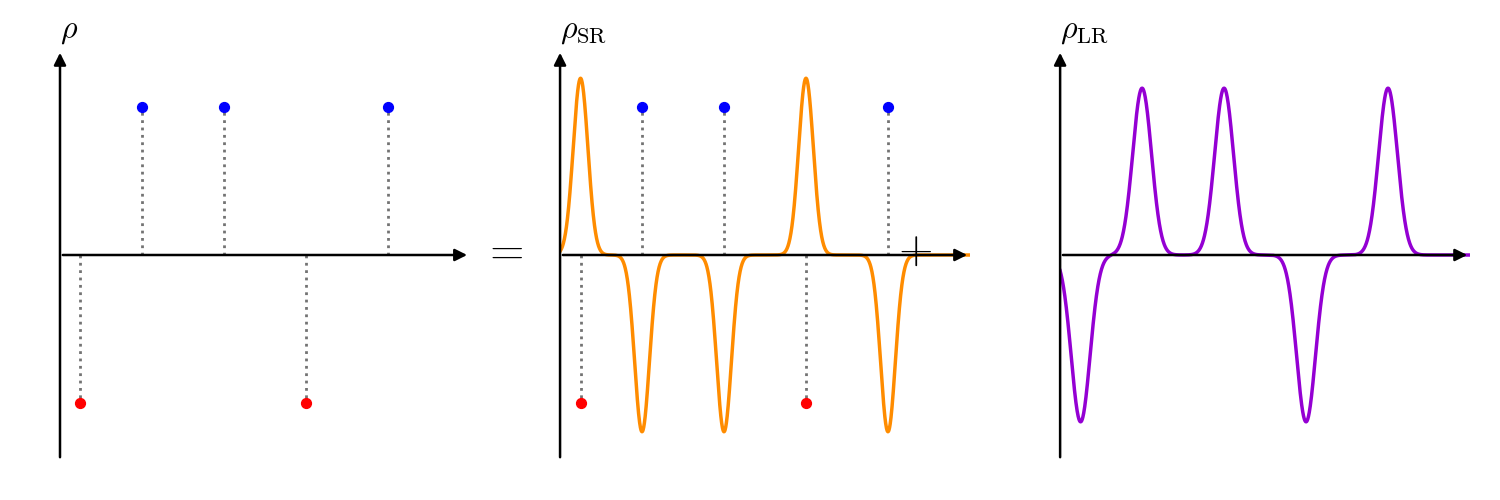
\includegraphics[width=1\linewidth]{General_Sections/Figures/pme.png}
    \caption{Charge distribution in the particle-mesh Ewald method. \textbf{(Left)} The charge density of point particles is that of a Dirac delta located in the position of the particle. The decomposition of the short and long-range contributions are equivalent to have \textbf{(center)} in the direct space the same distribution of Dirac-like charge density and a complementary Gaussian distribution, in the same position and with the same charge but opposite sign; and \textbf{(right)} Gaussian distribution of charges, with the same sign and magnitude as the original, in the reciprocal space. This treatment allows for a rapid convergence of the series, while keeping the periodicity of the system.}
    \label{fig:pme}
\end{figure}























\subsection{Force field resolution}

Force fields can be broadly classified according to their level of resolution, that is, according to how the molecular structure is represented and which atoms are treated as individual interaction sites. At the highest resolution are atomistic or all-atom (AA) force fields, such as Chemistry at Harvard Macromolecular Mechanics (CHARMM)~\cite{charmm}, Assisted Model Building with Energy Refinement (AMBER)~\cite{gaff}, and the Optimized Potentials for Liquid Simulations (OPLS) family~\cite{oplsaa}. In these models, atoms are represented explicitly, including hydrogen atoms. This level of resolution provides access to detailed structural and interaction features, which can be important when the phenomenon of interest depends on specific atomic interactions. However, the greater number of degrees of freedom also increases the computational cost of the simulations, particularly for systems containing large numbers of solvent molecules or extended assemblies such as lipid membranes. Although the direct evaluation of pairwise interactions would formally scale as $\mathcal{O}(N^2)$, practical MD implementations reduce this cost through techniques such as neighbor lists for short-range interactions and particle-mesh methods for long-range electrostatics~\cite{kim2023neighbor,pme}. The computational effort therefore depends not only on the number of particles, but also on the simulation algorithm, hardware, system size, and sampling protocol. Consequently, the accessible spatial and temporal scales of AA simulations are system-dependent and must be considered together with the sampling required to describe the process of interest. Importantly, higher structural resolution does not necessarily imply greater accuracy for every observable, since the quality of a force field ultimately depends on its parametrization, validation, and suitability for the system and phenomenon being studied~\cite{vangunsteren2018validation}.

An intermediate level of resolution is provided by united-atom (UA) force fields, in which selected groups of atoms are represented by a single interaction site. A common example is the GROningen MOlecular Simulation (GROMOS) force-field family~\cite{gromos}, where nonpolar hydrogen atoms can be incorporated into the corresponding heavy atoms, while atoms or groups for which explicit hydrogen representation is important can retain a higher level of detail. By reducing the number of interaction sites while retaining part of the chemical structure, UA models provide a compromise between the computational cost of fully atomistic descriptions and the structural detail required to represent molecular interactions.

A further reduction in resolution is achieved with coarse-grained (CG) force fields. In these models, several atoms are mapped onto a single interaction site, commonly referred to as a \textit{bead} (Figure~\ref{fig:AA2CG}). The reduction in the number of particles and degrees of freedom substantially decreases the computational cost and allows larger systems and longer trajectories to be investigated than would generally be practical with an equivalent atomistic description. This makes CG models particularly useful for processes involving large supramolecular assemblies or collective membrane phenomena, where the relevant length and timescales may extend beyond those readily accessible with AA simulations. The corresponding simplification, however, removes part of the atomistic detail and may limit the description of highly localized interactions or processes that depend on specific molecular geometries.

Among the CG force fields developed for biomolecular simulations, the Martini force field is one of the most widely used. Martini employs a systematic mapping in which groups of atoms are represented by interaction sites whose mapping and interaction properties depend on the molecular fragment and on the particular Martini version. Although a roughly 4:1 mapping is characteristic of many Martini 2 representations, the mapping is not universal and was modified in Martini 3~\cite{martini3}. The interaction sites are parameterized to reproduce selected thermodynamic properties rather than the complete atomistic potential-energy surface. This reduction in resolution provides a substantial computational advantage, while making the model particularly suitable for studying large biomolecular systems and processes occurring over extended spatial and temporal scales. The effective timescale accessible in a CG simulation nevertheless depends on the force-field version, integration timestep, system, hardware, and sampling protocol, and should therefore not be interpreted as a universal conversion from CG to physical time. Overall, the choice between AA, UA, and CG representations is best understood as a trade-off between molecular resolution, computational cost, and the level of detail required to address the scientific question.

\begin{figure}[!htbp]
    \centering
    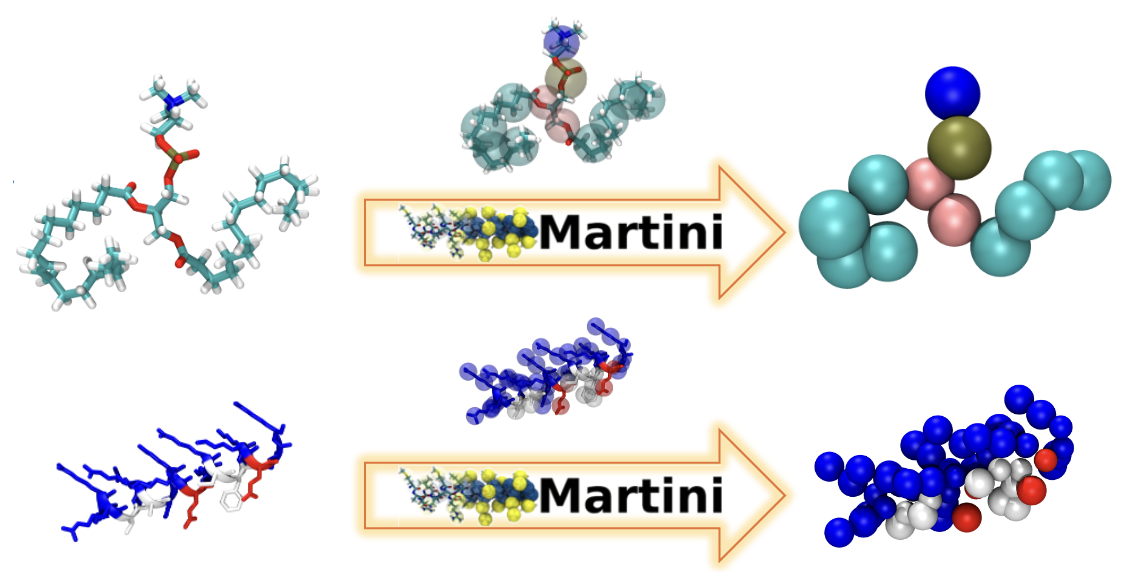
\includegraphics[width=0.99\linewidth]{General_Sections/Figures/AA2CG.png}
    \caption{Representation of the 3D structure of a lipid (up, POPC) and a peptide (bottom, KRRIRRAKKKEKRCFKKEKR) using an AA force field (left) and its corresponding mapping into Martini CG (right).}
    \label{fig:AA2CG}
\end{figure}

In the peptide--membrane simulations presented in the corresponding results chapter (see Section~\ref{art:metadynamics}), the Martini 2.2 coarse-grained force field~\cite{martini2} was employed to investigate the interaction and recognition mechanisms between AMPs and different biological membrane models. The use of a CG representation was motivated by the spatial and temporal scales associated with peptide--membrane recognition, which require extensive sampling and would therefore be computationally demanding with fully atomistic models. The reduced number of interaction sites and degrees of freedom substantially lowers the computational cost, making longer trajectories and larger membrane systems accessible.
The integration timestep in MD simulations is constrained by the fastest motions represented in the model, particularly high-frequency bond vibrations involving hydrogen atoms in atomistic descriptions~\cite{Feenstra1999}. Because these atomistic degrees of freedom are not explicitly represented in Martini, substantially larger integration timesteps can be used than in conventional AA-MD. For Martini 2.2, timesteps of 20--30~fs can be employed under appropriate simulation conditions, compared with the $\sim$2~fs commonly used in conventional AA-MD. This combination of reduced resolution and larger integration timesteps increases computational efficiency and facilitates simulations on the microsecond timescale.
Despite these advantages, conventional CG-MD may still be insufficient to efficiently sample rare peptide--membrane recognition events separated by free-energy barriers. To enhance sampling of these transitions, metadynamics was therefore combined with the CG-MD simulations. This approach promotes transitions between relevant conformational and configurational states and enables the reconstruction of the associated free-energy landscapes, providing a framework to characterize the energetics and specificity of peptide--membrane interactions.










\subsection{Metadynamics and free energy analysis}

\subsubsection{Standard metadynamics}

To understand the necessity of enhanced sampling methodologies, we must first establish the theoretical limitations of standard MD simulations. We consider a system governed by the conditions of the canonical ensemble. In this framework, the macroscopic state of the system is determined by the Helmholtz free energy, $A$, defined as:
\begin{equation}
    A = U - TS
\end{equation}
where $U$ is the internal energy, $T$ is the absolute temperature, and $S$ represents the entropy~\cite{termo_1,termo_2}. 

The mathematical justification for the approximation $\Delta A \approx \Delta G$ in condensed phases (liquids and solids) stems from the fundamental definitions of the relevant thermodynamic potentials. By definition, the Gibbs free energy ($G$) is expressed as:
\begin{equation}
    G = H - TS
\end{equation}
where $H$ is the enthalpy. The enthalpy itself is defined in terms of the internal energy, pressure ($P$), and volume ($V$) of the system:
\begin{equation}
    H = U + PV
\end{equation}

Substituting the definition of enthalpy into the equation for the Gibbs free energy yields:
\begin{equation}
    G = (U + PV) - TS = (U - TS) + PV
\end{equation}

Recognizing that the term $(U - TS)$ is precisely the definition of the Helmholtz free energy, we obtain the exact relationship between the two potentials:
\begin{equation}
    G = A + PV
\end{equation}

When analyzing a physical process or a transition between macroscopic states, the change in these thermodynamic potentials is denoted by the $\Delta$ operator:

\begin{equation}
    \Delta G = \Delta A + \Delta(PV)
\end{equation}

Applying the product rule, the expansion of the pressure-volume term gives $\Delta(PV) = P\Delta V + V\Delta P$. If the physical process occurs under typical experimental conditions at constant pressure (an isobaric process, where $\Delta P = 0$), the $V\Delta P$ term vanishes, and the equation simplifies to:
\begin{equation}
    \Delta G = \Delta A + P\Delta V
\end{equation}

For systems in condensed phases (liquids and solids), the materials are highly incompressible. Consequently, any volume change ($\Delta V$) during a chemical reaction, conformational transition, or thermal fluctuation is negligibly small ($\Delta V \approx 0$). Because the change in volume is minute, the mechanical work term $P\Delta V$ is physically insignificant compared to the characteristic magnitudes of the energetic and entropic contributions ($\Delta U$ and $T\Delta S$) involved in the process.

By neglecting the $P\Delta V$ term, we arrive at the condensed phase approximation~\cite{termo_1,termo_2}:
\begin{equation}
    \Delta G \approx \Delta A
\end{equation}

From a methodological standpoint, this derivation is crucial in computational physics and molecular simulation. It formally justifies why the results obtained from simulations in the canonical ensemble can be directly employed to study macroscopic processes that occur at constant pressure, which are governed by the Gibbs free energy~\cite{termo_1,termo_2}.

\paragraph{Equilibrium constants and ergodicity breaking}

When studying a system that transitions between two macroscopic states, $A$ and $B$, statistical mechanics dictates that the probability of observing the system in either state is proportional to its respective partition function~\cite{termo_1,termo_2}:
\begin{equation}
    P_A = \frac{Z_A}{Z}, \quad P_B = \frac{Z_B}{Z}
\end{equation}

The equilibrium constant, $K$, is defined as the ratio of these populations:
\begin{equation}
    K = \frac{P_B}{P_A} = \frac{Z_B}{Z_A}
\end{equation}

By relating the free energy of each state to its partition function ($A = -k_B T \ln Z$), the free energy difference between the two states, $\Delta A$, can be expressed entirely in terms of the equilibrium constant:
\begin{equation}
    \Delta A = A_B - A_A = -k_B T \ln Z_B + k_B T \ln Z_A = -k_B T \ln \frac{Z_B}{Z_A} = -k_B T \ln K
\end{equation}

This fundamental relationship demonstrates that $\Delta A$ fully determines the relative populations of the states and the equilibrium constant. Consequently, calculating the free energy surface (FES) along a chosen reaction coordinate, $\xi$, requires evaluating the marginal probability distribution, $P(\xi)$. This is achieved by integrating the Boltzmann factor over all degrees of freedom except $\xi$~\cite{termo_1,termo_2}:
\begin{equation}
    Z(\xi) = \frac{\int \delta[\xi'(r) - \xi] e^{-\beta E} d^N r}{\int e^{-\beta E} d^N r}
\end{equation}
where the denominator is the total partition function and the numerator evaluates the integral restricted to microstates where the system's coordinates $r$ correspond to the value $\xi$.

In a standard MD simulation, phase space is explored through a single, continuous time trajectory~\cite{termo_metad_presion,termo_1,termo_2}. Under the ergodic hypothesis, commonly assumed in statistical mechanics for systems at thermodynamic equilibrium, the ensemble average equates to the time average in the limit of infinite simulation time:
\begin{equation}
    Z(\xi) = P(\xi) = \lim_{t \to \infty} \frac{1}{t} \int_0^t \rho[\xi(t')] dt'
\end{equation}

However, the probability of visiting a specific configuration with energy $E$ is dictated by the Boltzmann distribution, $P(E) \propto \exp\left(-\frac{E}{k_B T}\right)$~\cite{termo_1,termo_2}. Because this probability is exponentially sensitive to energy, low-energy regions are sampled correctly, whereas high-energy transition states are rarely visited. When a system possesses high energy barriers ($\Delta A \gg k_B T$), the time required to spontaneously cross these barriers vastly exceeds feasible simulation lengths. Consequently, the assumption of infinite simulation time breaks down, ergodicity is broken, and the exact calculation of $\Delta A$ using standard MD becomes impossible.
Conventional MD simulations are often hindered by the timescale problem, trapping the system in local minima of the FES separated by high free-energy barriers~\cite{Laio2002}. To overcome this timescale bottleneck, various enhanced sampling methods have been proposed, such as Replica Exchange MD, Steered MD, and Umbrella Sampling. However, these methods may require extensive prior knowledge of the system, scale poorly with complex reaction coordinates, or lack adaptability~\cite{termo_metad_presion}.

This limitation motivated the development of history-dependent biasing methods, most notably metadynamics (MetaD)~\cite{termo_metad_presion}. Rather than waiting for the system to spontaneously cross high free-energy barriers, MetaD accelerates the exploration of the free-energy landscape by introducing a history-dependent bias potential along a set of predefined slow degrees of freedom, known as collective variables (CVs), denoted as $\vec{s}(\vec{q})$.

The basic idea is to progressively discourage the system from revisiting regions of CV space that have already been explored. This is achieved by depositing small repulsive Gaussian potentials along the trajectory at regular time intervals. As these Gaussians accumulate, previously visited free-energy minima are progressively filled, reducing the effective barriers and promoting transitions to less explored regions of the CV space. In this sense, MetaD can be viewed as a dynamical biasing scheme that progressively flattens the free-energy landscape along the selected CVs.

Instead of evolving solely under the original potential energy function $U(\vec{q})$, the system evolves under a time-dependent biased potential:
\begin{equation}
U_{\mathrm{bias}}(\vec{q},t)
=
U(\vec{q}) + V(\vec{s}(\vec{q}),t)
\end{equation}
where $V(\vec{s},t)$ is the history-dependent bias potential acting on the selected CVs~\cite{termo_metad_presion}.

The bias potential is constructed as a sum of Gaussian kernels periodically deposited along the trajectory in CV space:
\begin{equation}\label{eq:metad_bias}
V(\vec{s},t)
=
\sum_{k\tau < t}
W(k\tau)
\exp\left[
-\sum_{i=1}^{d}
\frac{
\left(s_i-s_i(\vec{q}(k\tau))\right)^2
}{2\sigma_i^2}
\right]
\end{equation}
where $\tau$ is the deposition stride, $W(k\tau)$ is the height of the Gaussian deposited at time $k\tau$, and $\sigma_i$ is its width along the $i$-th CV. Here, $\vec{q}(k\tau)$ denotes the microscopic coordinates of the system at the deposition time, such that $s_i(\vec{q}(k\tau))$ defines the center of the corresponding Gaussian in CV space.

The statistical-mechanical basis of MetaD follows from the relationship between the equilibrium probability distribution of the CVs, $P(\vec{s})$, and the corresponding free-energy surface:
\begin{equation}
F(\vec{s}) = -k_{\mathrm{B}}T\ln P(\vec{s}) + C
\end{equation}
where $C$ is an arbitrary additive constant. By continuously modifying the sampling distribution through the accumulated bias, MetaD reduces the probability of repeatedly visiting already sampled regions and promotes exploration of higher free-energy regions.

Under the assumption that the selected CVs provide a suitable description of the slow degrees of freedom and that the bias is deposited sufficiently slowly, the accumulated bias approaches the negative of the underlying free-energy surface in CV space. In the long-time limit,
\begin{equation}
V(\vec{s},t\rightarrow\infty)
\approx
-F(\vec{s}) + C
\end{equation}
Consequently, the biased free-energy landscape becomes approximately flat along the selected CVs, allowing the system to explore regions that would be rarely visited in an unbiased simulation. The accumulated bias can therefore be used to reconstruct the underlying free-energy surface and estimate the relative thermodynamic stability of the sampled states without requiring prior knowledge of the transition pathways~\cite{termo_metad_presion}.

\begin{figure}[!htbp]
    \centering
    \includesvg[width=0.65\linewidth]{General_Sections/Figures/metadynamics_comparison.svg}
    \caption{Progressive evolution of a one-dimensional model potential $V(s)$ by metadynamics bias. The thick black curve is the starting potential with two wells and a central barrier. Thin colored lines (from dark purple to yellow) represent the dynamic evolution of the sum of Gaussians along a trajectory that first explores the left well, then crosses the barrier, and finally visits the right well.}
    \label{fig:metad}
\end{figure}




\subsubsection{Well-Tempered metadynamics}

In standard metadynamics, Gaussian bias potentials of fixed height are continuously deposited along the selected collective variables (CVs), progressively discouraging the system from revisiting previously sampled regions of the CV space. This promotes the exploration of configurations separated by free-energy barriers. However, the continuous deposition of Gaussians can lead to persistent fluctuations in the accumulated bias and does not result in the same asymptotic behavior as Well-Tempered Metadynamics (WTMetaD).

WTMetaD introduces a bias-dependent scaling of the Gaussian height, such that the magnitude of newly deposited Gaussians decreases as the bias accumulates~\cite{Barducci2008}. The height of a Gaussian deposited at time $t=k\tau$ is given by:

\begin{equation}
W (k \tau ) = W_0 \exp \left( -\frac{V(\vec{s}(\vec{q}(k \tau)),k \tau)}{k_B\Delta T} \right )
\end{equation}

where $W_0$ is the initial Gaussian height, $V(\vec{s},t)$ is the accumulated bias potential, $k_B$ is the Boltzmann constant, and $\Delta T$ is a parameter controlling the rate at which the Gaussian height decreases.

The degree of tempering is commonly expressed through the bias factor $\gamma$,

\begin{equation}
\gamma
=
\frac{T+\Delta T}{T}
\end{equation}

The parameter $\Delta T$ does not represent an actual increase in the physical temperature of the system. Instead, it controls the extent to which the sampling distribution is broadened along the biased CVs. In the long-time limit, the WTMetaD bias converges, up to an additive constant, to a fraction of the underlying free-energy surface:

\begin{equation}
V(\vec{s},t\rightarrow \infty) = -\frac{\Delta T}{T+\Delta T}F(\vec{s}) + C = -\left(1 - \frac{1}{\gamma}\right)F(\vec{s}) + C
\end{equation}

where $F(\vec{s})$ is the free-energy surface and $C$ is an arbitrary constant. Thus, the bias factor determines the degree to which the free-energy landscape is compensated during the simulation. In the limit $\gamma\rightarrow1$, the biasing effect vanishes, whereas increasing $\gamma$ progressively approaches the behavior of standard MetaD~\cite{Barducci2008}.

\paragraph{Practical considerations and limitations}
Despite its theoretical guarantees, the performance of (WT)MetaD in practice depends critically on several methodological choices. First, the quality of the reconstructed free-energy surface is inherently limited by the choice of CVs: if the selected variables do not capture all relevant slow degrees of freedom, important free-energy barriers may remain unsampled and the resulting FES will be incomplete~\cite{Bussi2020}. Second, the deposition parameters (Gaussian height $W_0$, width $\sigma_i$, and stride $\tau$) must be chosen carefully. Excessively large or narrow Gaussians can lead to over-biasing or insufficient resolution of the free-energy surface, respectively. Third, although WTMetaD is guaranteed to converge to a well-defined stationary distribution, convergence can be slow for high-dimensional CV spaces or systems with multiple competing slow modes. In practice, convergence is assessed by monitoring the time evolution of the accumulated bias and verifying that free-energy profiles computed from successive portions of the trajectory become stationary~\cite{termo_metad_presion}.

\subsubsection{Thermodynamic reweighting}

Because the system evolves under a time-dependent bias, the configurations generated during a WTMetaD simulation are sampled from a distribution that differs from the unbiased canonical ensemble. Statistical reweighting can therefore be used to account for the effect of the applied bias when estimating thermodynamic observables.

If the biased Hamiltonian is written as:

\begin{equation}
H'(\vec{q},\vec{p},t)
=
H(\vec{q},\vec{p})
+
V(\vec{s}(\vec{q}),t)
\end{equation}

the corresponding statistical weight required to recover the unbiased distribution is related to the Boltzmann factor of the bias. For a given configuration, the reweighting factor can be expressed schematically as:

\begin{equation}
w(\vec{q},t)
\propto
\exp\left[
\frac{V(\vec{s}(\vec{q}),t)}
{k_B T}
\right]
\end{equation}

These weights allow observables to be estimated from the biased trajectory while accounting for the effect of the metadynamics potential. In particular, they can be used to reconstruct free-energy profiles along coordinates different from those directly biased during the simulation, provided that the relevant regions of configurational space have been sufficiently sampled. Reweighting does not compensate for insufficient sampling and therefore cannot recover information about configurations or regions of phase space that were not adequately explored.



\subsubsection{Selection and formulation of collective variables}

The success of an enhanced sampling calculation depends critically on the choice of collective variables (CVs). Ideally, the selected CVs should capture the slow or otherwise relevant degrees of freedom associated with the transitions between the metastable states of interest. An inappropriate choice of CVs may result in inefficient sampling or hinder the reconstruction of the underlying free-energy landscape~\cite{Bussi2020}. In the study of AMP--membrane interactions, CVs are commonly defined as geometric descriptors of the association and orientation of the peptide relative to the membrane. For example, peptide--membrane distance and orientational variables such as tilt or rotation angles can be used to characterize the main degrees of freedom involved in membrane recognition and insertion~\cite{DANI_METADINAMICA}.

\paragraph{Geometrical framework of the peptide--membrane system}

To define the CVs used to characterize peptide--membrane association, the system is described geometrically in a three-dimensional Cartesian coordinate system, with the $z$-axis defined as the normal to the membrane plane. The peptide and membrane are represented by their respective centers of mass (COM), together with vectors describing the orientation of the peptide relative to the membrane.

\textbf{Distance and insertion depth.} Let $\vec{R}_{\mathrm{mem}}$ and $\vec{R}_{\mathrm{pep}}$ denote the centers of mass of the membrane and peptide, respectively. For a set of particles with masses $m_i$ and positions $\vec{r}_i$, the center of mass is given by:

\begin{equation}
\vec{R}_{\mathrm{mem}} = \frac{1}{M_{\mathrm{mem}}} \sum_{i\in\mathrm{mem}} m_i\vec{r}_i,
\qquad
\vec{R}_{\mathrm{pep}} = \frac{1}{M_{\mathrm{pep}}} \sum_{j\in\mathrm{pep}} m_j\vec{r}_j
\end{equation}

where:

\begin{equation}
M_{\mathrm{mem}}=\sum_{i\in\mathrm{mem}}m_i,
\qquad
M_{\mathrm{pep}}=\sum_{j\in\mathrm{pep}}m_j
\end{equation}

are the corresponding total masses. The peptide--membrane separation vector is then defined as:

\begin{equation}
\vec{D} = \vec{R}_{\mathrm{pep}} - \vec{R}_{\mathrm{mem}}
\end{equation}

The component of this vector along the membrane normal,

\begin{equation}
D_z = \vec{D}\cdot\hat{z}
\end{equation}

provides a measure of the peptide's position along the membrane-normal direction and is therefore used as a CV for the translational component of membrane association. The corresponding Euclidean distance between the two centers of mass is:

\begin{equation}
D = ||\vec{D}|| = \sqrt{D_x^2+D_y^2+D_z^2}
\end{equation}

While $D$ describes the overall separation between the peptide and membrane COMs, $D_z$ specifically characterizes their relative displacement along the membrane normal. For a membrane lying approximately in the $xy$ plane, this coordinate provides a direct measure of the peptide's approach towards and displacement across the bilayer along the principal insertion direction.

\paragraph{Peptide orientation and tilt angle}

The orientation of the peptide relative to the membrane is characterized by an internal peptide axis defined from the centers of mass of the N- and C-terminal residues. Let $\vec{N}$ and $\vec{C}$ denote these positions,

\begin{equation}
\vec{N} = \vec{r}_{\mathrm{N-term}},
\qquad
\vec{C} = \vec{r}_{\mathrm{C-term}}
\end{equation}

The peptide axis is then defined as:

\begin{equation}
\vec{h} = \vec{C}-\vec{N},
\qquad
\hat{h} = \frac{\vec{h}}{||\vec{h}||}
\end{equation}

The \textbf{tilt angle} $\theta$ is defined as the angle between the peptide axis and the membrane normal $\hat{z}$:

\begin{equation}
\theta =
\arccos\left(\hat{h}\cdot\hat{z}\right)
\end{equation}

Thus, $\theta=0^\circ$ corresponds to an orientation in which the peptide axis is parallel to the membrane normal, whereas $\theta=90^\circ$ corresponds to an orientation in which the peptide axis lies parallel to the membrane plane. In this definition, $\theta$ characterizes the inclination of the peptide with respect to the membrane and therefore provides the principal rotational coordinate associated with its orientation.

\paragraph{Internal rotation around the peptide axis}

The tilt angle alone does not fully specify the orientation of an elongated peptide. In particular, two peptides with the same $\theta$ can differ in the orientation of their side-chain distribution around the longitudinal axis. To describe this degree of freedom, an internal rotation angle $\phi$ is introduced.

A molecular reference vector $\hat{\mu}$ is first defined from the peptide backbone and projected onto the plane perpendicular to the peptide axis,

\begin{equation}
\hat{\mu}_{\perp} = \frac{ \hat{\mu}-(\hat{\mu}\cdot\hat{h})\hat{h} }{ \left| \hat{\mu}-(\hat{\mu}\cdot\hat{h})\hat{h} \right| }
\end{equation}

A reference direction within the plane perpendicular to $\hat{h}$ is defined using the membrane normal, and a second orthogonal direction is obtained as (based on the definition by Esteban-Martín and Salgado~\cite{ESTEBANMARTIN20074278}):


\begin{equation}
\hat{t} = \hat{h}\times \frac{ \hat{z}\times\hat{h} }{ |\hat{z}\times\hat{h}| }
\end{equation}


The internal rotation angle can then be expressed using the two components of $\hat{\mu}_{\perp}$ in this local reference frame ((Figure \ref{fig:eulers_angles})):
 \begin{equation}
\phi = \mathrm{sgn}\left( \hat{h} \cdot (\hat{t} \times \hat{\mu}_\perp) \right) \cdot \arccos\left( \hat{\mu}_\perp \cdot \hat{t} \right)
\end{equation}
where the sign correction ensures a continuous mapping of the full $360^\circ$ rotation. Periodic boundary conditions are taken into account when constructing all position vectors involved in these calculations.

The reference frame becomes singular when $\hat{h}$ is parallel to $\hat{z}$, since $|\hat{z}\times\hat{b}|=0$. This corresponds to the limiting case $\theta=0^\circ$. In practice, configurations approaching this singularity are handled by imposing a minimum norm threshold when constructing the local frame.

\paragraph{Relevant orientational degrees of freedom}

The orientation of the peptide with respect to the membrane can be described by three rotational coordinates. The tilt angle $\theta$ specifies the inclination of the peptide axis relative to the membrane normal, while $\phi$ specifies the rotation of the molecular structure around that axis. A third angle would describe the azimuthal direction of the peptide axis within the membrane plane (Figure \ref{fig:eulers_angles}).

For the present system, this latter coordinate is not included as a collective variable because the membrane plane does not provide a fixed in-plane reference direction for the peptide. In particular, for a homogeneous and laterally isotropic membrane, a global rotation of the system within the membrane plane does not change the relative membrane--peptide configuration. The relevant orientational information can therefore be represented by the tilt and internal rotation angles.

Together with the translational coordinate $D_z$, the CV space used to characterize peptide--membrane association is therefore defined by (see Section \ref{art:metadynamics}):

\begin{equation}
\left(D_z,\theta,\phi\right)
\end{equation}

which captures the peptide displacement along the membrane normal, its inclination relative to the membrane, and its rotation around its longitudinal axis. These coordinates provide a reduced geometrical description of the principal translational and orientational changes involved in peptide association with the membrane.


\begin{figure}[!ht]
    \centering
    \includesvg[width=0.75\linewidth]{General_Sections/Figures/helix_geometry.svg}
    \caption{Definition of the generalized coordinates $q$ for a helical peptide in a 3-D coordinate system.
    The peptide (represented by the blue helix) is modeled as a rigid body whose configuration is fully described by a set of generalized coordinates $q \in \mathbb{R}^6$. This set comprises three translational degrees of freedom, $(x, y, z)$, and three rotational degrees of freedom, $(\psi, \theta, \phi)$, corresponding to the Euler angles. 
    The translation coordinates $(x, y)$ denote the position of the peptide within the membrane plane, while $z$ represents the insertion depth along the membrane normal. Regarding orientation, $\theta$ (tilt angle) defines the inclination relative to the $Z$-axis, $\psi$ (azimuthal angle) describes the orientation of the tilt in the $XY$ plane, and $\phi$ represents the internal rotation of the helix about its longitudinal axis $\mathbf{\hat{n}}$. 
    Assuming an infinite, homogeneous, and isotropic membrane in the $XY$ plane, the system exhibits translational symmetry along $X$ and $Y$, as well as rotational symmetry around the $Z$-axis. Consequently, the potential energy of the system is independent of $x, y$, and $\psi$ (ignorable coordinates), effectively reducing the configurational study to the three biologically relevant degrees of freedom: insertion depth ($z$), tilt ($\theta$), and internal rotation ($\phi$).}
    \label{fig:eulers_angles}
\end{figure}



\subsubsection{Dimensionality reduction of free energy surfaces}

A free-energy surface (FES) obtained from multiple collective variables can be projected onto a lower-dimensional space when only a subset of the variables is required for a particular analysis. Such a projection must account for the statistical weight associated with the degrees of freedom that are integrated out. Consequently, a thermodynamic projection cannot, in general, be obtained by taking a cross-section of the original FES or by selecting the minimum-energy value along the discarded coordinate.

For a two-dimensional FES $F(s_1,s_2)$, the corresponding equilibrium probability density in the collective-variable space is related to the free energy through the Boltzmann relation,

\begin{equation}
F(s_1,s_2) = -k_B T \ln P(s_1,s_2) + C
\end{equation}

where $k_B$ is the Boltzmann constant, $T$ is the temperature, and $C$ is an arbitrary additive constant. Equivalently,

\begin{equation}
P(s_1,s_2)
\propto
\exp\left[
-\frac{F(s_1,s_2)}{k_B T}
\right]
\end{equation}

The thermodynamic projection onto $s_1$ is obtained by marginalizing the probability density over the discarded variable $s_2$:

\begin{equation}
P(s_1) = \int P(s_1,s_2)\,ds_2
\end{equation}

Substituting the Boltzmann relation gives:

\begin{equation}
P(s_1)
\propto
\int
\exp\left[
-\frac{F(s_1,s_2)}{k_B T}
\right]
ds_2
\end{equation}

The corresponding one-dimensional free-energy profile is then obtained from the marginal probability,

\begin{equation}
F(s_1) = -k_B T\ln P(s_1)+C'
\end{equation}

or, equivalently,

\begin{equation}
F(s_1) = -k_B T \ln \left[ \int \exp\left( -\frac{F(s_1,s_2)}{k_B T} \right) ds_2 \right] +C''
\end{equation}

where $C''$ absorbs the normalization constants. This expression shows that the projected free energy accounts for the statistical contribution of all configurations along the discarded coordinate. In contrast, a minimum-energy projection would retain only the lowest value of $F(s_1,s_2)$ at each $s_1$ and therefore would not preserve the corresponding configurational entropy.

In practice, the resulting profile is defined up to an arbitrary additive constant. For visualization and comparison, it is therefore conventional to shift the profile such that its minimum is equal to zero.


\paragraph{Computational implementation}

In practice, thermodynamic projections of multidimensional free-energy surfaces can be obtained during post-processing using the \texttt{sum\_hills} utility of the PLUMED package. When a subset of the collective variables is specified using the \texttt{--idw} option, the remaining variables are integrated out in the reconstruction of the free-energy surface. The corresponding thermal energy, $k_B T$, must be provided through the \texttt{--kt} option in energy units consistent with those used for the bias potential~\cite{plumed}.

For example, a two-dimensional FES defined by $s_1$ and $s_2$ can be projected onto $s_1$ using

\begin{verbatim}
plumed sum_hills --hills HILLS --idw s1 --kt 2.5
\end{verbatim}

Here, \texttt{--idw s1} specifies $s_1$ as the variable retained in the projected FES, while the remaining CV, $s_2$, is integrated out. The \texttt{--kt} value specifies the thermal energy used in this integration. Consequently, the resulting one-dimensional profile corresponds to a thermodynamic marginalization over the discarded CV rather than to a simple minimum-energy projection~\cite{plumed}.




\subsubsection{Calculation of the standard binding free energy ($\Delta G^0$)}

The FES obtained from enhanced-sampling simulations provides a description of the relative stability of the peptide configurations sampled along the selected collective variables. To quantify the thermodynamic affinity of a peptide for a membrane and to facilitate comparison between different membrane models, a standard Gibbs free energy of binding, $\Delta G^0$, can be obtained by integrating the corresponding potential of mean force (PMF) and applying a standard-state correction~\cite{Woo2005}.

From statistical thermodynamics, the probability of observing a microscopic state with energy $W$ at temperature $T$ is proportional to its Boltzmann factor,

\begin{equation}
p \propto e^{-\beta W}
\end{equation}

where $\beta=(k_B T)^{-1}$, with $k_B$ denoting the Boltzmann constant. For a peptide interacting with a membrane, the configurational state can in general be described by its translational coordinates $\vec{r}$ and orientational degrees of freedom $\Upsilon$. The corresponding configurational partition function per unit volume can be expressed as:

\begin{equation}
\frac{q}{V}
=
\frac{1}{V}
\int
e^{-\beta W(\vec{r},\Upsilon)}
d\vec{r},d\Upsilon
\end{equation}

The partition coefficient $\kappa$ between the bound ($b$) and free ($f$) states is defined as the ratio of their probabilities per unit volume,

\begin{equation}
\kappa
=
\frac{p_b/V_b}{p_f/V_f}
=
\frac{q_b/V_b}{q_f/V_f}
\end{equation}

For the peptide--membrane system considered here, the PMF is projected onto the membrane-normal coordinate $z$, with the bulk region defined such that the peptide--membrane interaction is negligible beyond a distance $\lambda$. Under this one-dimensional approximation, the partition coefficient is obtained from the Boltzmann-weighted integral of the PMF,

\begin{equation}
\kappa
=
\frac{1}{\lambda}
\int_0^\lambda
e^{-\beta W(z)}
,dz
\end{equation}

where $\lambda$ defines the range of the membrane-associated region considered in the calculation. The corresponding free energy of association is:

\begin{equation}
\Delta G
=
-k_B T\ln(\kappa)
\end{equation}

To express this quantity relative to the conventional standard concentration of $1$ M, a standard-state correction is introduced. The volume corresponding to one molecule at a concentration of $1$ M is:

\begin{equation}
V_0
=
\frac{1}{C_0}
=
\frac{1~\mathrm{L}}{N_A}
\approx
1660~\text{\AA}^3
\end{equation}

where $C_0=1$ M and $N_A$ is Avogadro's constant. Because the PMF is expressed along a one-dimensional reaction coordinate, the corresponding standard-state length scale is given by $V_0^{1/3}$. Following the formulation used for peptide--membrane adsorption~\cite{DANI_CUANTICA}, the standard-state partition coefficient is therefore:

\begin{equation}
\kappa^0
=
\kappa
\frac{\lambda}{V_0^{1/3}}
=
\frac{1}{V_0^{1/3}}
\int_0^\lambda
e^{-\beta W(z)}
,dz
\end{equation}

The standard Gibbs free energy of binding is subsequently calculated as:

\begin{equation}
\Delta G^0
=
-k_B T\ln(\kappa^0)
\end{equation}

This formulation provides a standard-state free energy of peptide--membrane association based on the PMF along the membrane-normal coordinate. The resulting value depends on the definition of the bound and reference regions and on the one-dimensional approximation adopted for the calculation. Consequently, comparisons with experimental binding free energies should be interpreted within the same thermodynamic and state definitions.



















\section{Statistical methods and error analysis}

Molecular dynamics simulations generate trajectories consisting of a large number of configurations sampled over time. The analysis of these trajectories involves calculating averages, fluctuations, correlations, and other statistical quantities from the sampled data. Because consecutive configurations are generally correlated, the statistical information contained in a trajectory cannot be assessed solely from the total number of recorded frames. Appropriate statistical treatment is therefore required both to obtain representative estimates of the properties of interest and to quantify their associated uncertainties~\cite{tratamiento_datos_fisicos}.

In this work, statistical analysis is applied to the time series and structural data obtained from the molecular dynamics simulations. The methods described in this section include the calculation of temporal averages, the treatment of statistical uncertainty arising from autocorrelation through block averaging, and dimensionality-reduction and clustering techniques used to characterize the conformational space explored by the simulations. These approaches provide the basis for the quantitative analysis of the simulated systems and the identification of distinct conformational states.



\subsection{Sample and temporal averages}

For a set of $N$ discrete observations of a quantity $x$, the sample mean is defined as:
\begin{equation}
\langle x \rangle = \frac{1}{N}\sum_{n=1}^{N}x_n
\end{equation}
When the quantity is expressed as a function of time, $x(t)$, its temporal average over a time interval $T$ is given by:
\begin{equation}
\bar{x} =
\frac{1}{T}
\int_{t_0}^{t_0+T} x(t'),dt'
\end{equation}
In practice, MD trajectories provide discrete observations separated by a sampling interval $\Delta t$. The temporal average can therefore be approximated by the arithmetic mean of the sampled trajectory frames:
\begin{equation}
\bar{x}
\approx
\frac{1}{N}
\sum_{n=1}^{N}
x(t_0+n\Delta t)
\end{equation}
where $T=N\Delta t$. Here, $\Delta t$ denotes the interval between consecutive observations used for the analysis and does not necessarily correspond to the integration time step of the MD simulation. In particular, coordinates and other observables are typically saved less frequently than the integration step in order to limit data storage and avoid redundant sampling.


\subsection{The autocorrelation problem and block averaging}
Most of the analyses performed in this work generate time series of physical quantities. To extract statistically meaningful conclusions from these data, it is necessary to quantify the uncertainty associated with the calculated averages. Following the treatment by Gómez Rodríguez et al.~\cite{tratamiento_datos_fisicos}, for a set of $N$ observations, the dispersion of the data is characterized by the sample variance $s^2(x)$, estimated as:
\begin{equation}
s^2(x) =
\frac{1}{N-1}
\sum_{n=1}^{N}
\left(x_n-\langle x\rangle\right)^2
\label{eq:variance}
\end{equation}
where $\langle x\rangle$ is the sample mean. The corresponding sample standard deviation, $s(x)=\sqrt{s^2(x)}$, characterizes the fluctuations of individual observations around the mean.
For error estimation, however, it is necessary to distinguish $s(x)$ from the standard deviation of the mean, or standard error, denoted as $\sigma_{\langle x\rangle}$. This quantity represents the uncertainty associated with the estimated average. If the $N$ observations were statistically independent and uncorrelated, the standard error would be given by:
\begin{equation}
\sigma_{\langle x\rangle}
=
\frac{s(x)}{\sqrt{N}}
\label{eq:std_error}
\end{equation}

A fundamental challenge in molecular dynamics simulations is that consecutive observations in a trajectory are generally not statistically independent, but instead exhibit temporal correlations. Consequently, the assumption underlying equation~\ref{eq:std_error} is not valid for correlated trajectories. Using the total number of frames $N$ in this case leads to an underestimation of the statistical uncertainty, because the effective number of independent observations is smaller than the total number of recorded frames.
To account for these correlations, the Block Averaging method was employed following the procedure introduced by Flyvbjerg and Petersen~\cite{block_average}. The original data set of $N$ observations is divided into $N'=N/k$ consecutive blocks of size $k$. The mean of each block $i$ is calculated as:
\begin{equation}
M_i =
\frac{1}{k}
\sum_{j=1}^{k}
x_{(i-1)k+j}
\end{equation}
The resulting block averages constitute a new statistical sample with a reduced number of observations. As the block size $k$ is progressively increased, correlations between neighboring block averages are reduced. The statistical error of the mean is evaluated as a function of the block size, and a plateau in the estimated error indicates convergence of the statistical uncertainty, suggesting that the remaining correlations between blocks are negligible.
Following the blocking analysis, the final uncertainty $\sigma$ and its associated statistical uncertainty $\sigma_{\sigma}$ are estimated as:
\begin{equation}
\sigma
\approx
\sqrt{\frac{s^2(M)}{N'-1}},
\qquad
\sigma_{\sigma}
\approx
\frac{\sigma}{\sqrt{2(N'-1)}}
\end{equation}
where $s^2(M)$ denotes the variance of the set of block averages and $N'$ is the number of blocks at the selected block size. The second expression provides an estimate of the statistical uncertainty associated with the calculated error itself.
This procedure accounts for the temporal correlations present in MD trajectories and therefore provides a more reliable estimate of the uncertainty associated with trajectory-derived quantities than the assumption of statistically independent observations. It was consequently used to estimate the statistical uncertainties reported for the free-energy surfaces and other quantities derived from the simulations.




\subsection{Principal component analysis}
Principal Component Analysis (PCA) is a fundamental statistical method in multivariate analysis that performs a linear transformation of the coordinate system. From a mathematical perspective, PCA is a change of basis that maps the data from its original high-dimensional space to a new orthogonal coordinate system whose axes are ordered according to the amount of variance they capture.
Let us consider a data set consisting of $n$ observations and $d$ variables, represented by a data matrix $\mathbf{X} \in \mathbb{R}^{n \times d}$. To ensure that the covariance matrix describes the fluctuations around the mean, the data are first centered such that each variable has zero mean:
\begin{equation}
[\mathbf{X}]_{ij} \leftarrow [\mathbf{X}]_{ij} - \bar{x}_j
\end{equation}
where $\bar{x}_j$ is the mean of the $j$-th variable. The covariance between these variables is then described by the covariance matrix $\mathbf{C} \in \mathbb{R}^{d \times d}$, defined as:
\begin{equation}
\mathbf{C} = \frac{1}{n-1} \mathbf{X}^T \mathbf{X} =
\begin{pmatrix}
\mathrm{Var}(x_1) & \mathrm{Cov}(x_1,x_2) & \cdots & \mathrm{Cov}(x_1,x_d) \\
\mathrm{Cov}(x_2,x_1) & \mathrm{Var}(x_2) & \cdots & \mathrm{Cov}(x_2,x_d) \\
\vdots & \vdots & \ddots & \vdots \\
\mathrm{Cov}(x_d,x_1) & \mathrm{Cov}(x_d,x_2) & \cdots & \mathrm{Var}(x_d)
\end{pmatrix}
\end{equation}
The diagonal elements represent the variance of each individual variable, whereas the off-diagonal elements represent the covariance between pairs of variables. Non-zero covariance values indicate that fluctuations in different variables are statistically related and therefore contain overlapping information.
The core objective of PCA is to identify a new set of orthogonal axes, known as principal directions, along which the variance of the data is maximized and the projected variables are mutually uncorrelated. These directions are obtained by diagonalizing the covariance matrix through an eigenvalue decomposition:
\begin{equation}
\mathbf{C}\mathbf{V} = \mathbf{V}\mathbf{\Lambda}
\end{equation}
where $\mathbf{V}$ is an orthogonal matrix whose columns are the eigenvectors $\vec{v}_i$, and $\mathbf{\Lambda}$ is a diagonal matrix containing the corresponding eigenvalues $\lambda_i$. The eigenvectors define the directions of the principal axes, while the corresponding eigenvalues quantify the variance of the data along those directions.
The original data can then be projected onto the principal directions according to:
\begin{equation}
\mathbf{Y} = \mathbf{X}\mathbf{V}
\end{equation}
The columns of $\mathbf{Y}$ are the principal component scores, representing the coordinates of the observations in the new basis. Because the covariance matrix is diagonal in this basis, these projected variables are mutually uncorrelated. The eigenvectors are conventionally ordered according to decreasing eigenvalue,
\begin{equation}
\lambda_1 \geq \lambda_2 \geq \dots \geq \lambda_d
\end{equation}
so that the first principal components account for the largest fractions of the total variance. Consequently, the dimensionality of the data can be reduced by retaining only the first few components, thereby obtaining a lower-dimensional representation while preserving as much of the original variance as possible.

\subsection{K-means clustering}
To further characterize the conformational states of a molecular system and identify representative structures, clustering methods such as K-means can be applied to molecular dynamics trajectories. K-means is an unsupervised learning algorithm that partitions a set of observations into $K$ distinct clusters according to their proximity in the selected feature space~\cite{MacQueen1967,Lloyd1982}. In MD analysis, the observations may correspond to trajectory frames represented by Cartesian coordinates, principal component scores, or other collective variables.
The K-means algorithm iteratively minimizes the within-cluster sum of squares (WCSS), also referred to as inertia. Given an initial set of $K$ centroids, each observation is represented by a feature vector $\vec{x}_i$ and assigned to the cluster with the nearest centroid $\vec{\mu}_j$. The centroids are then recalculated as the mean of the feature vectors assigned to each cluster, and the procedure is repeated until the cluster assignments or centroids converge. The objective function can be written as:

\begin{equation}
    \min_{\{S_j\}_{j=1}^{K}}
    \sum_{j=1}^{K}
    \sum_{\vec{x}_i \in S_j}
    \left\|
    \vec{x}_i-\vec{\mu}_j
    \right\|^2
\end{equation}

where $S_j$ denotes the $j$-th cluster. The objective is therefore to minimize the sum of squared Euclidean distances between each observation and the centroid of its assigned cluster.




























































%%%%%%% CONTINUAR
\section{Quantum computing}
A central computational challenge in the study and design of antimicrobial peptides is the enormous size of the sequence and conformational spaces that must be considered. For a peptide of length \(L\), the number of possible sequences composed of the 20 standard amino acids grows exponentially as \(20^L\), making exhaustive enumeration impractical even for relatively short peptides~\cite{Levinthal_paradox,robert2021resource}. Moreover, each sequence can adopt multiple three-dimensional conformations, whose relative stability and accessibility depend on the molecular environment. This dependence is particularly relevant for membrane-active peptides, for which the conformational ensemble can change substantially upon interaction with lipid interfaces~\cite{paper_paula,vogel_amps}.

The difficulty of exploring such conformational spaces is commonly illustrated by the Levinthal paradox~\cite{Levinthal_paradox,Levinthal_paradox_2}. An exhaustive and unbiased sampling of all possible conformations would require an astronomically large number of configurations, incompatible with the timescales observed for protein and peptide folding. The resolution of this apparent paradox is that molecular folding does not proceed through a random enumeration of all possible conformations. Instead, the physical interactions between residues constrain the accessible conformational pathways and give rise to a highly non-uniform energy landscape~\cite{Levinthal_paradox,robert2021resource,Levinthal_paradox_2}. Nevertheless, identifying the relevant low-energy states and characterizing the transitions between them remains computationally challenging, particularly when several slow degrees of freedom and environmental interactions contribute to the dynamics.


\subsection{Computational challenges and the NISQ era}
The computational complexity of biomolecular optimization can also be considered from the perspective of formal complexity theory. Protein folding and related structure-prediction problems have been shown to be computationally difficult under several simplified formulations, including lattice models and contact-map representations~\cite{robert2021resource}. These results should not be interpreted as a direct proof that continuous molecular dynamics is NP-hard. Rather, they illustrate the combinatorial nature of simplified formulations of the underlying optimization problem. In practical molecular simulations, the main difficulty arises from the combination of a large configuration space, complex energy landscapes, and the computational cost required to sample them adequately.
Machine-learning (ML) methods provide an alternative strategy by learning relationships between sequence, structure, and experimentally or computationally derived properties. AlphaFold, for example, demonstrated that deep-learning models can predict protein structures with high accuracy for many classes of proteins~\cite{Jumper2021}. Such approaches, however, primarily target structure prediction rather than explicit simulation of the physical pathways connecting conformational states. Consequently, they do not directly provide molecular free-energy landscapes or dynamical trajectories, and their treatment of environment-dependent interactions depends on the information represented in the model and its training data. These considerations are particularly relevant for peptide--membrane systems, where lipid composition, interfacial environment, and conformational transitions can play a central role~\cite{PROTEINMPNN,ROSETTA,Goverde2024,dolorfino2024,platform_ia_2,ia_lim_big}.
ML-based approaches have also been applied to the exploration and optimization of peptide sequence space. For example, ApexGO combines generative modelling with Bayesian optimization to identify peptide sequences with predicted improvements in antimicrobial activity~\cite{Torres2026}. In this framework, sequence optimization is driven by a learned predictor of minimum inhibitory concentration rather than by an explicit physical energy function. Consequently, the optimization is constrained by the properties represented in the predictor and by the distribution of sequences and experimental conditions available to the underlying model~\cite{Torres2026}. This illustrates a general distinction between data-driven and physics-based approaches: ML methods can efficiently navigate large sequence spaces, whereas their predictions and optimization objectives remain dependent on the scope and assumptions of the learned models.
Physics-based approaches, such as MD, explicitly evaluate molecular interactions according to a predefined molecular-mechanics force field and provide access to conformational dynamics and, with appropriate sampling methods, to thermodynamic quantities. Their applicability is nevertheless constrained by the computational cost of evaluating the potential energy and by the difficulty of sampling processes separated by high free-energy barriers or involving slow collective variables. These limitations become particularly relevant for peptide--membrane recognition, where association, reorientation, insertion, and conformational changes may occur on different timescales~\cite{computational_expensive_MD}. Thus, MD and ML provide complementary approaches: ML can efficiently explore large data-defined spaces, whereas physics-based simulations provide an explicit model of the interactions governing the sampled molecular dynamics.
These complementary limitations motivate the investigation of alternative computational formulations in which selected molecular problems can be expressed as energy-based optimization problems. QC provides a framework for representing and manipulating such optimization problems using quantum states and quantum operations. In an $N$-qubit system, the state is represented in a $2^N$-dimensional Hilbert space~\cite{nielsen2010quantum,robert2021resource}. This exponential state-space dimension, however, does not imply that all $2^N$ amplitudes can be directly accessed or that every problem formulated on a quantum computer obtains a computational advantage. Any potential advantage depends on the specific encoding, quantum algorithm, cost function, and measurement strategy~\cite{nielsen2010quantum,preskill1998quantum}.
The present work is situated within the Noisy Intermediate-Scale Quantum (NISQ) era, in which quantum processors operate with limited numbers of noisy qubits and without the full fault-tolerant error correction required for large-scale quantum algorithms~\cite{preskill1998quantum}. Practical performance is therefore affected by hardware noise, qubit connectivity, gate fidelity, circuit depth, coherence times, and the number of measurements required to estimate the relevant observables~\cite{Shor1995,KITAEV20032}. Accordingly, the objective of the quantum-computing component of this work is not to establish quantum advantage, but to investigate how selected peptide-related problems can be formulated as quantum optimization problems and to assess the associated computational requirements and limitations under currently available hardware and simulation conditions.


\subsection{Foundations of quantum information}
To understand the application of quantum algorithms to molecular design, it is useful to first introduce the basic units of quantum information and the mathematical operations used to manipulate them. Quantum information theory provides a framework for encoding and processing information according to the principles of quantum mechanics, using quantum states and operations that differ fundamentally from their classical counterparts~\cite{nielsen2010quantum,preskill1998quantum}.
\subsubsection{Qubits and multi-qubit systems}
The fundamental unit of quantum information is the quantum bit, or \textit{qubit}. Analogously to a classical bit, a qubit has two orthogonal computational basis states, conventionally denoted by $|0\rangle$ and $|1\rangle$. Physically, these two states can be encoded in different quantum systems, such as two energy levels of an atom, the internal states of an ion, or the states of a superconducting circuit~\cite{nielsen2010quantum,preskill1998quantum}.
Qubits are mathematically represented using Dirac's \textit{ket} notation. A common representation of the computational basis states is given by the column vectors:
\begin{equation}
|0\rangle =
\begin{pmatrix}
1\\
0
\end{pmatrix},
\qquad
|1\rangle =
\begin{pmatrix}
0\\
1
\end{pmatrix}
\end{equation}
Unlike a classical bit, whose state is restricted to either $0$ or $1$, a qubit can be described as a coherent linear combination of the two computational basis states. A general pure qubit state is therefore written as:
\begin{equation}
|\psi\rangle = \alpha|0\rangle + \beta|1\rangle =
\begin{pmatrix}
\alpha\\
\beta
\end{pmatrix}
\end{equation}
where $\alpha,\beta\in\mathbb{C}$ are complex probability amplitudes. The state must satisfy the normalization condition:
\begin{equation}
|\alpha|^2+|\beta|^2=1
\end{equation}
such that $|\alpha|^2$ and $|\beta|^2$ correspond to the probabilities of obtaining the respective computational basis states upon measurement.
The state space of multiple qubits is constructed through the tensor product of the individual qubit Hilbert spaces. For a system of $N$ qubits, the corresponding Hilbert space is:
\begin{equation}
\mathcal{H}_N=(\mathbb{C}^2)^{\otimes N}
\end{equation}
which has dimension $2^N$. Its computational basis consists of all binary strings of length $N$, denoted by $z\in\{0,1\}^N$. Consequently, a general pure state of the system can be expressed as:
\begin{equation}
|\psi\rangle =
\sum_{z\in\{0,1\}^N}
\alpha_z |z\rangle,
\qquad
\text{with}
\qquad
\sum_{z\in\{0,1\}^N}|\alpha_z|^2=1
\end{equation}
where each $\alpha_z\in\mathbb{C}$ is the probability amplitude associated with the computational basis state $|z\rangle$. The normalization condition ensures that the probabilities of all possible measurement outcomes sum to unity~\cite{nielsen2010quantum,preskill1998quantum}.
A single-qubit pure state can also be represented geometrically on the surface of the unit sphere, known as the Bloch sphere (see Figure~\ref{fig:bloch_sphere}). Up to an overall global phase, any pure qubit state can be parameterized by two angles, $\theta$ and $\phi$, as:
\begin{equation}
|\psi\rangle =
\cos\left(\frac{\theta}{2}\right)|0\rangle
+
e^{i\phi}
\sin\left(\frac{\theta}{2}\right)|1\rangle,
\qquad
0\leq\theta\leq\pi,
\qquad
0\leq\phi<2\pi
\end{equation}
The corresponding Bloch vector is:
\begin{equation}
\vec{r}=
\left(
\sin\theta\cos\phi,
\sin\theta\sin\phi,
\cos\theta
\right)
\end{equation}
where $\theta$ determines the polar angle with respect to the $Z$ axis and $\phi$ determines the azimuthal angle in the $XY$ plane. The computational basis states $|0\rangle$ and $|1\rangle$ correspond to the north and south poles of the sphere, respectively, as illustrated in Figure~\ref{fig:bloch_sphere}.

\begin{figure}[!htbp]
    \centering
    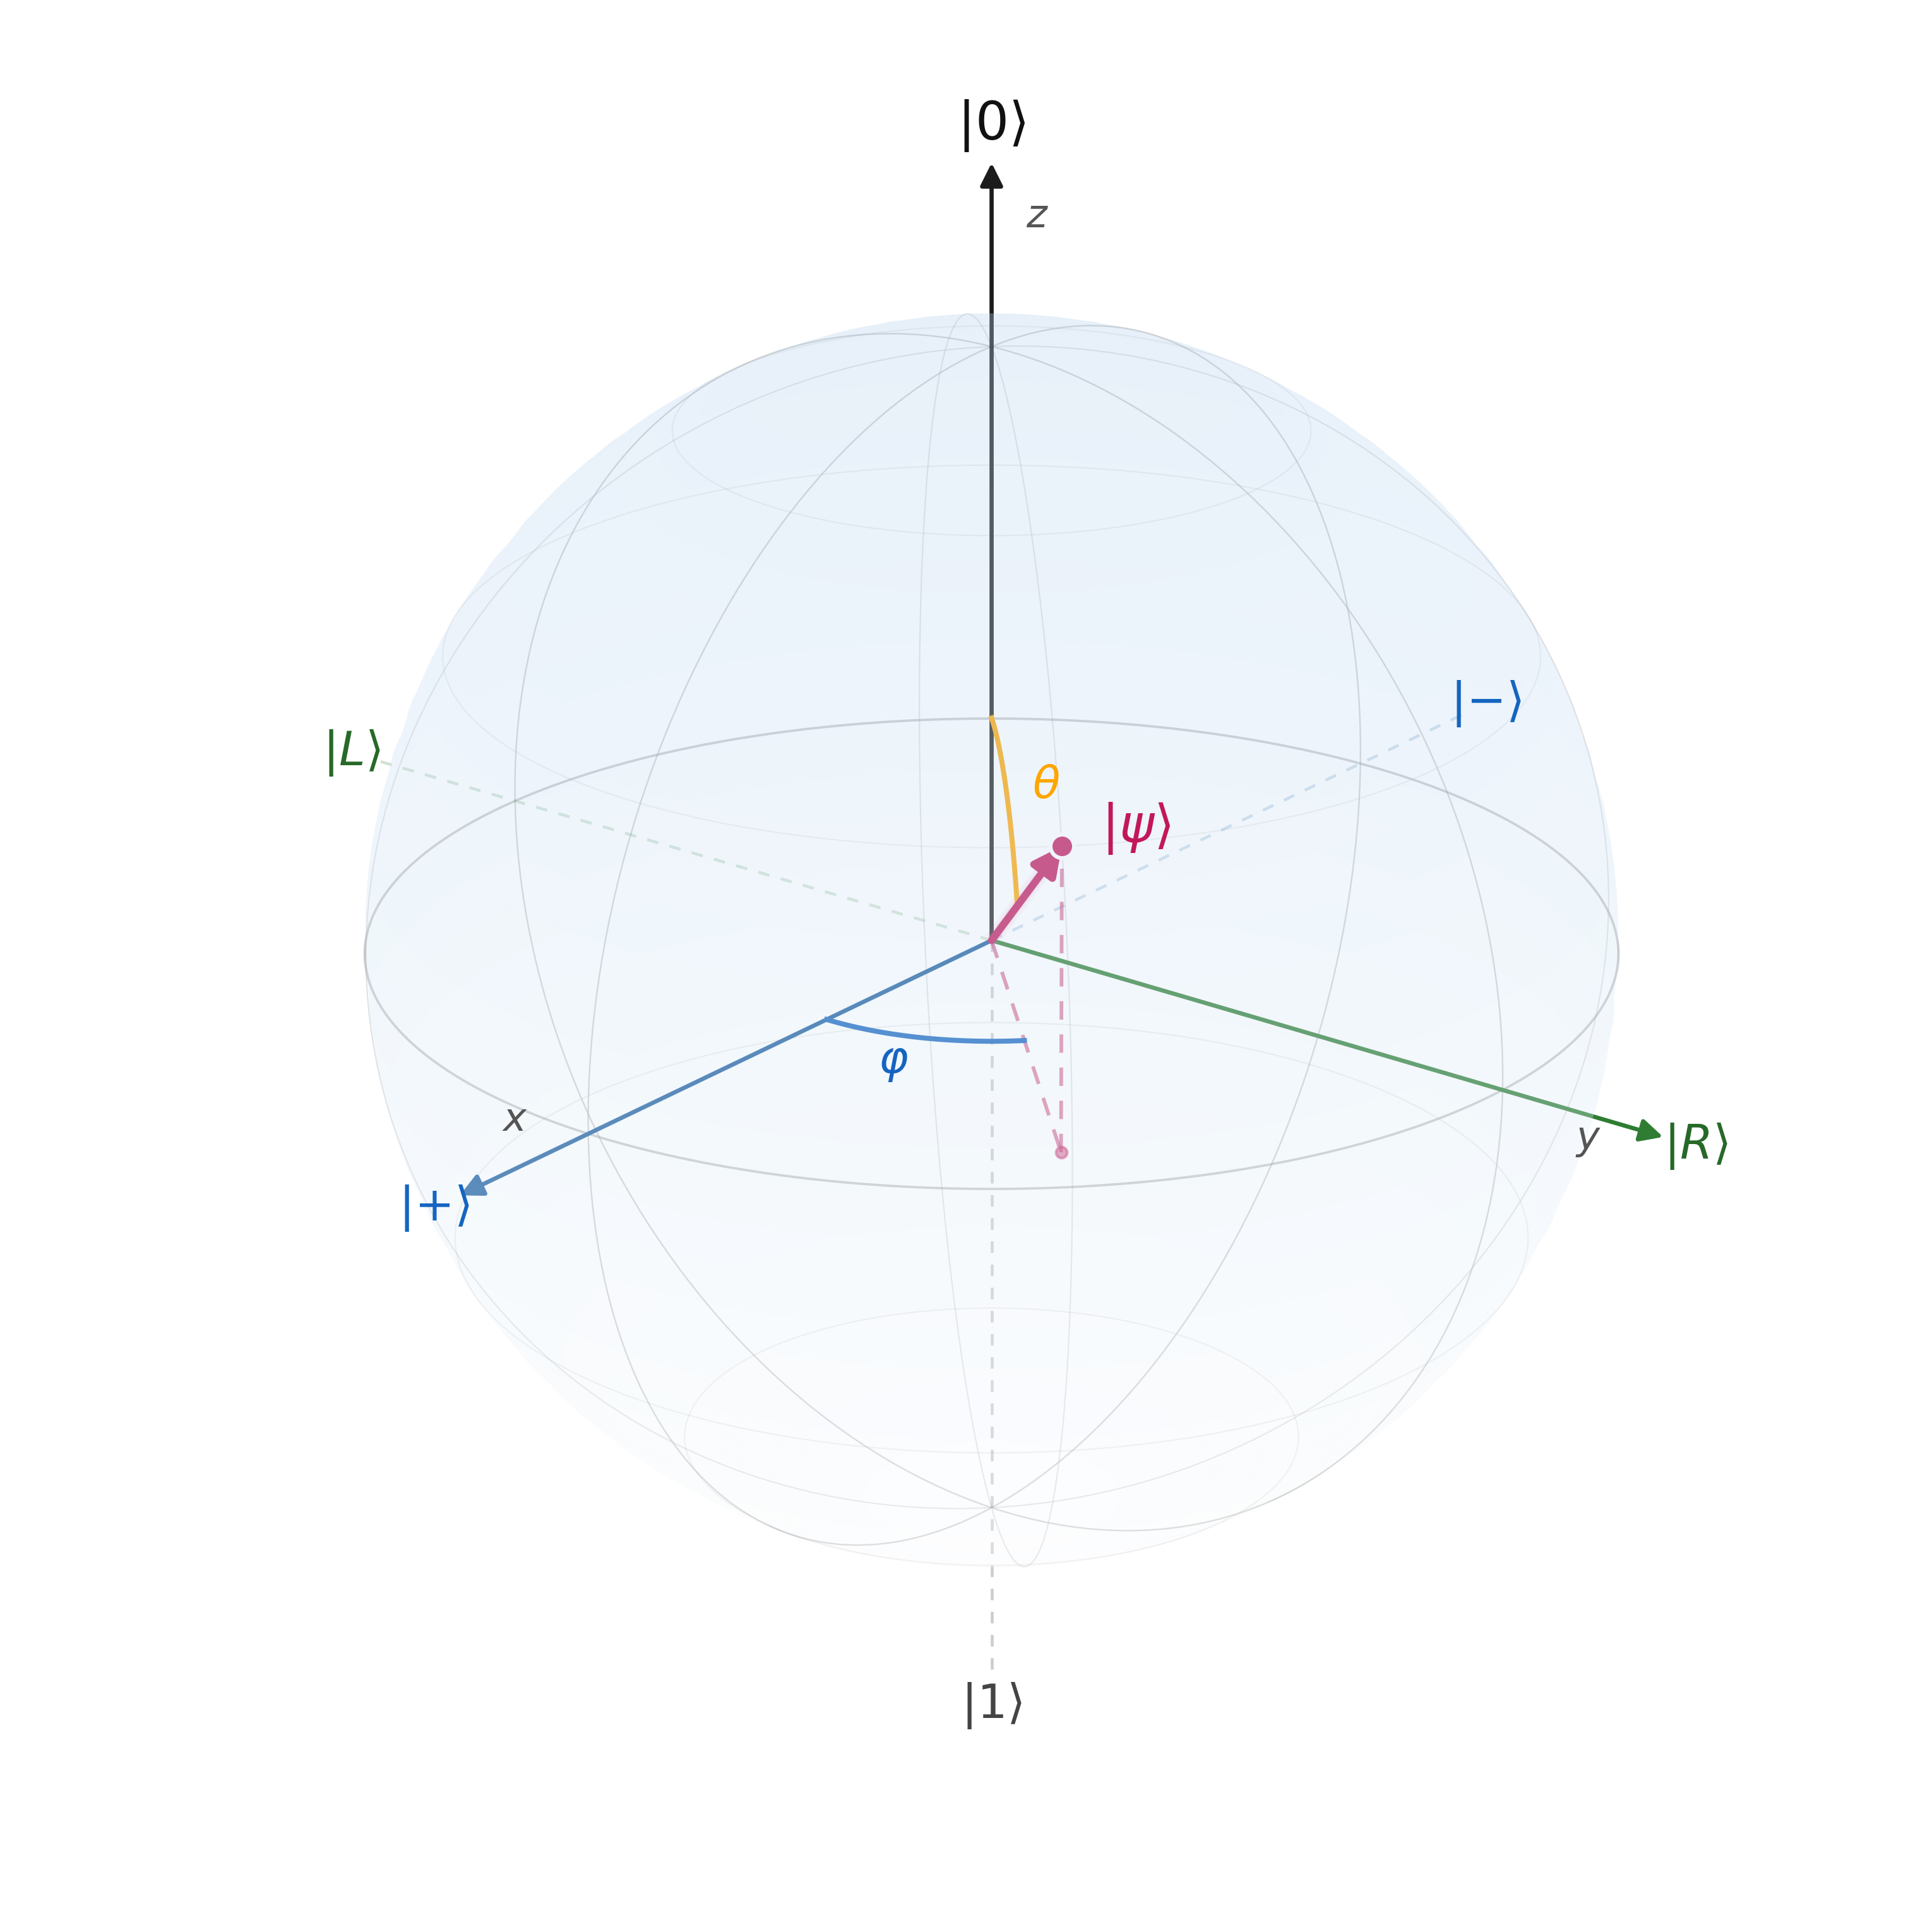
\includegraphics[width=0.6\linewidth]{General_Sections/Figures/esfera_bloch_tesis.png}
    \caption{The Bloch sphere representation of a single-qubit state. The angles $\theta$ and $\phi$ determine the position of the state vector on the surface of the sphere. The $Z$-axis corresponds to the computational basis states $|0\rangle$ and $|1\rangle$, while the $X$ and $Y$ axes describe the relative coherence and phase between their probability amplitudes.}
    \label{fig:bloch_sphere}
\end{figure}

\subsubsection{Unitary dynamics and quantum gates}
Analogous to classical computers, which employ elementary logic gates such as AND or NOT to perform deterministic operations on bits, quantum computers use quantum gates to manipulate the states and probability amplitudes of one or more qubits. The continuous-time evolution of a closed quantum system is governed by the time-dependent Schr\"odinger equation (adopting natural units such that $\hbar=1$)~\cite{nielsen2010quantum}:
\begin{equation}
i\frac{d|\psi(t)\rangle}{dt}=\hat{H}|\psi(t)\rangle
\end{equation}
The Hamiltonian operator $\hat{H}$ is the observable associated with the total energy of the quantum system. Its eigenstates $|\psi_i\rangle$ and corresponding eigenvalues $E_i$ satisfy:
\begin{equation}
\hat{H}|\psi_i\rangle=E_i|\psi_i\rangle
\end{equation}
For an $N$-qubit system, $\hat{H}$ is a $2^N\times2^N$ Hermitian operator. Its eigenstates form an orthonormal basis of the Hilbert space, in which the Hamiltonian admits the spectral decomposition:
\begin{equation}
\hat{H}=\sum_{i=1}^{2^N}E_i|\psi_i\rangle\langle\psi_i|
\end{equation}
When the Hamiltonian is time-independent, the formal solution of the Schr"odinger equation can be expressed through the unitary time-evolution operator:
\begin{equation}
\hat{U}(t)=e^{-i\hat{H}t}
\end{equation}
such that an initial state $|\psi(0)\rangle$ evolves according to:
\begin{equation}
|\psi(t)\rangle=\hat{U}(t)|\psi(0)\rangle
\end{equation}
Because $\hat{U}(t)$ is unitary, it preserves inner products and, consequently, the normalization of the quantum state. In gate-based quantum computing, general unitary transformations are implemented through sequences of discrete quantum gates. These gates therefore provide the elementary operations used to construct quantum circuits and approximate or synthesize the desired unitary evolution.

\paragraph{Pauli and rotation gates}
The Pauli operators constitute a fundamental set of single-qubit operators and form the basis for many quantum operations and Hamiltonian representations. They are both Hermitian and unitary:
\begin{equation}
\sigma_x \equiv X = \begin{pmatrix} 0 & 1 \\ 1 & 0 \end{pmatrix}, \quad 
\sigma_y \equiv Y = \begin{pmatrix} 0 & -i \\ i & 0 \end{pmatrix}, \quad 
\sigma_z \equiv Z = \begin{pmatrix} 1 & 0 \\ 0 & -1 \end{pmatrix}
\end{equation}
The Pauli-$X$ operator acts as a bit-flip, analogous to the classical NOT operation, mapping:
\begin{equation}
X|0\rangle=|1\rangle,
\qquad
X|1\rangle=|0\rangle
\end{equation}
The Pauli-$Z$ operator leaves $|0\rangle$ unchanged while introducing a relative phase of $\pi$ to $|1\rangle$:
\begin{equation}
Z|0\rangle=|0\rangle,
\qquad
Z|1\rangle=-|1\rangle
\end{equation}
Another fundamental single-qubit gate is the Hadamard gate, $H$, which transforms computational basis states into equal superpositions:
\begin{equation}
H=\frac{1}{\sqrt{2}}
\begin{pmatrix}
1&1\\
1&-1
\end{pmatrix}
\end{equation}
with:
\begin{equation}
H|0\rangle=|+\rangle=
\frac{|0\rangle+|1\rangle}{\sqrt{2}},
\qquad
H|1\rangle=|-\rangle=
\frac{|0\rangle-|1\rangle}{\sqrt{2}}
\end{equation}
These states lie on the equator of the Bloch sphere and constitute the eigenstates of the Pauli-$X$ operator.
Parameterized rotation gates provide continuous control over the state of a qubit and are particularly important in variational quantum algorithms. They are defined as:
\begin{equation}
R_x(\theta)=e^{-i\theta X/2},
\qquad
R_y(\theta)=e^{-i\theta Y/2},
\qquad
R_z(\theta)=e^{-i\theta Z/2}
\end{equation}
For example, the $R_z$ gate introduces a relative phase between the computational basis states:
\begin{equation}
R_z(\theta)=
\begin{pmatrix}
e^{-i\theta/2}&0\\
0&e^{i\theta/2}
\end{pmatrix}
\end{equation}
\paragraph{Two-qubit gates and entanglement}
Single-qubit gates alone cannot generate entanglement from an initially separable state. Two-qubit gates, in contrast, can create correlations that cannot be represented as a product of independent single-qubit states. A fundamental example is the controlled-NOT (CNOT) gate, which flips a target qubit $q_t$ if and only if the control qubit $q_c$ is in the state $|1\rangle$:
\begin{equation}
CNOT=
\begin{pmatrix}
1&0&0&0\\
0&1&0&0\\
0&0&0&1\\
0&0&1&0
\end{pmatrix}
\end{equation}
For example, applying a CNOT gate to the separable state $|+\rangle\otimes|0\rangle$ produces the Bell state:
\begin{equation}
|+\rangle|0\rangle
\xrightarrow{CNOT}
\frac{|00\rangle+|11\rangle}{\sqrt{2}}
\end{equation}
which is an entangled state. This illustrates how two-qubit gates provide the mechanism for introducing entanglement into quantum circuits, a resource that plays a central role in many quantum algorithms.

\subsubsection{Measurement and hardware architectures}
Unlike classical readout, quantum measurement in the computational basis is a non-unitary and probabilistic process that projects the quantum state onto one of the computational basis states~\cite{nielsen2010quantum,preskill1998quantum}. For a state:
\begin{equation}
|\psi\rangle=\sum_z\alpha_z|z\rangle
\end{equation}
a measurement in the computational basis returns a particular classical bitstring $z$ with probability $|\alpha_z|^2$.
Because a measurement produces a single probabilistic outcome, the quantum state must generally be prepared repeatedly to characterize its underlying probability distribution. Repeated measurements, commonly referred to as \textit{shots}, yield a histogram of bitstrings from which measurement probabilities can be estimated. These probabilities should be distinguished from expectation values of observables. For an observable $\hat{O}$, its expectation value is estimated from the measurement outcomes as:
\begin{equation}
\langle\hat{O}\rangle
\approx
\frac{1}{N_{\mathrm{shots}}}
\sum_{k=1}^{N_{\mathrm{shots}}}o_k
\end{equation}
where $o_k$ denotes the measurement outcome associated with the $k$-th shot. The statistical standard error of this estimator is:
\begin{equation}
\sqrt{\frac{\mathrm{Var}(\hat{O})}{N_{\mathrm{shots}}}}
\end{equation}
showing that the statistical uncertainty decreases as $1/\sqrt{N_{\mathrm{shots}}}$~\cite{mcclean2016theory}. Thus, increasing the number of measurements improves the statistical precision, but does not by itself eliminate systematic errors arising from state-preparation, gate, or measurement imperfections.
For a Hamiltonian expressed as a weighted sum of measurable operators,
\begin{equation}
\hat{H}=\sum_j c_j\hat{P}_j
\end{equation}
where $\hat{P}_j$ are typically tensor products of Pauli operators, its expectation value can be reconstructed from the individual expectation values,
\begin{equation}
\sum_j c_j\langle\hat{P}_j\rangle
\end{equation}
This decomposition is particularly important for variational quantum algorithms, in which the expectation value of the Hamiltonian is repeatedly estimated from finite sets of measurements.
\paragraph{Hardware platforms}
Several physical architectures have been developed to implement qubits, each with different trade-offs in coherence, gate speed, connectivity, scalability, and experimental complexity.
\begin{itemize}
\item \textbf{Trapped-ion architecture:} Individual ions are confined in vacuum using electromagnetic fields, typically in radio-frequency Paul traps. Qubits are encoded in internal electronic or hyperfine states, while quantum gates are implemented using laser or microwave interactions. The shared vibrational modes of the ions can mediate high-fidelity entangling operations and provide long-range connectivity within an ion chain~\cite{trapped_ions}.

\item \textbf{Superconducting qubits:} These qubits are implemented using cryogenic superconducting circuits containing Josephson junctions. They offer fast gate operations and can be fabricated using established micro- and nanofabrication techniques, making them attractive for large-scale integration. Their main challenges include relatively short coherence times compared with some other platforms, control errors, crosstalk, and the requirement for sophisticated cryogenic infrastructure~\cite{superconductiong_qubits}.

\item \textbf{Photonic quantum computing:} Quantum information is encoded in properties of photons such as polarization, path, or temporal modes. Photonic systems offer low sensitivity to thermal environments and can operate without cryogenic cooling for many components. However, photon loss, efficient state generation and detection, and the implementation of deterministic two-photon interactions remain important experimental challenges. Entangling operations can therefore rely on measurement-based approaches, interference, or specialized nonlinear optical components~\cite{photonic_qubits}.
\end{itemize}



\subsection{Variational Quantum Algorithms}
Variational quantum algorithms (VQAs) constitute a class of hybrid quantum--classical algorithms designed to operate on near-term quantum hardware. Rather than relying exclusively on long, fully quantum circuits, VQAs distribute the computational workload between a Quantum Processing Unit (QPU) and a classical processor. The quantum processor prepares parameterized quantum states and evaluates the corresponding objective function through measurements, while a classical optimizer updates the circuit parameters based on the measured results~\cite{preskill1998quantum}. This iterative structure allows variational algorithms to operate with circuit depths compatible with current quantum hardware, although their performance remains constrained by hardware noise, circuit depth, measurement overhead, and the efficiency of the classical optimization procedure.
The implementation of VQAs is facilitated by software frameworks that provide tools for quantum-circuit construction, simulation, compilation, execution, and classical optimization. In this research, two complementary frameworks were primarily employed:
\begin{itemize}
\item \textbf{Qiskit}~\cite{Qiskit}: an open-source quantum computing framework developed by IBM that provides tools for constructing, simulating, transpiling, and executing quantum circuits on simulators and IBM quantum hardware.
\item \textbf{PennyLane}~\cite{pennylane}: a cross-platform framework for differentiable quantum programming that integrates quantum circuits with classical computational workflows. Its automatic-differentiation capabilities facilitate the optimization of parameterized quantum circuits using gradient-based and other classical optimization methods.
\end{itemize}
Within this thesis, two VQA-based approaches are considered for distinct optimization problems. The Variational Quantum Eigensolver (VQE) is employed to investigate peptide conformational optimization by encoding the corresponding energy function into a qubit Hamiltonian and minimizing its expectation value~\cite{DANI_CUANTICA}. The Quantum Approximate Optimization Algorithm (QAOA), in contrast, is employed to address discrete amino-acid sequence optimization under environment-dependent objectives~\cite{DANI_HAMILTONIAN}. Thus, VQE is used here to address an energy-minimization problem over a parameterized quantum state, whereas QAOA is used to explore a discrete combinatorial optimization landscape. The formulation, encoding strategy, ansatz, optimization procedure, and computational backend used for each problem are described separately in the corresponding results chapters (see Section~\ref{art:vqe_cesga} and \ref{art:hamiltonian}).



\subsubsection{Hamiltonians and parameterized circuits}
To formulate a physical or mathematical optimization problem on a quantum computer, its objective function must be encoded in terms of operators acting on a register of qubits. In the context of VQAs, this is commonly achieved by expressing the Hamiltonian $\hat{H}$ as a linear combination of tensor products of single-qubit Pauli operators.
The Pauli operators $X$, $Y$, and $Z$, together with the identity operator $I$, form a basis for the real vector space of Hermitian $2\times2$ operators. Consequently, any Hermitian operator acting on an $n$-qubit register can be expressed as a linear combination of tensor products of these single-qubit operators. The resulting set of $4^n$ Pauli strings forms a basis for the space of Hermitian operators acting on the $n$-qubit Hilbert space:
\begin{equation}
\hat{H} = \sum_i w_i P_i,
\qquad
P_i\in\{I,X,Y,Z\}^{\otimes n}
\end{equation}
where $w_i\in\mathbb{R}$ are the corresponding coefficients. This decomposition is central to VQAs because the expectation value of each Pauli string can be estimated experimentally through measurements in an appropriate basis, allowing the expectation value of the full Hamiltonian to be reconstructed from a finite set of measurable quantities.
The structure of the Hamiltonian depends on the optimization problem being considered. In VQE, $\hat{H}$ represents a physical or effective energy operator whose ground-state energy is sought and may contain non-commuting Pauli terms. According to the variational principle, the expectation value of the Hamiltonian for any normalized trial state provides an upper bound to the ground-state energy. In QAOA, the objective function is encoded in a cost Hamiltonian $\hat{H}_C$, which is typically diagonal in the computational basis and can therefore be expressed using products of $Z$ operators. The QAOA circuit additionally employs a mixer Hamiltonian, $\hat{H}_M$, which introduces transitions between computational-basis states.
The quantum state explored during a VQA is generated by a parameterized unitary circuit, commonly referred to as an \textit{ansatz}. Formally, the trial state is written as:
\begin{equation}
|\psi(\boldsymbol{\theta})\rangle = U(\boldsymbol{\theta})|0\rangle^{\otimes n}
\end{equation}
where $\boldsymbol{\theta}$ denotes the set of classical variational parameters. A commonly used circuit architecture is a layered ansatz,
\begin{equation}
U(\boldsymbol{\theta}) = \prod_{l=1}^{L}U_l(\boldsymbol{\theta}_l)
\end{equation}
where each layer may contain parameterized single-qubit rotations and entangling operations. The choice of ansatz determines the variational manifold accessible to the circuit and therefore represents an important compromise between expressibility, number of parameters, circuit depth, and susceptibility to optimization and hardware-related limitations~\cite{nielsen2010quantum}.
For a Hamiltonian decomposed into Pauli strings, the VQA objective function is given by:
\begin{equation}
C(\boldsymbol{\theta}) = \sum_i w_i
\langle\psi(\boldsymbol{\theta})|
P_i
|\psi(\boldsymbol{\theta})\rangle
\end{equation}
For VQE, minimizing this expectation value with respect to the variational parameters yields an approximation to the ground-state energy:
\begin{equation}
E_0
\leq
\min_{\boldsymbol{\theta}}
C(\boldsymbol{\theta})
\end{equation}
where $E_0$ denotes the exact ground-state energy. In practice, the individual expectation values $\langle P_i\rangle$ are estimated from repeated measurements of the quantum circuit. These measurements are combined according to the coefficients $w_i$ to evaluate the objective function, which is subsequently optimized by a classical optimization procedure.



\subsubsection{The Variational Quantum Eigensolver}
The Variational Quantum Eigensolver (VQE) is a hybrid quantum--classical algorithm designed to approximate the ground-state energy of a Hamiltonian~\cite{vqe_mejor}. Its theoretical basis is the Rayleigh--Ritz variational principle, which states that, for any normalized trial state $|\psi(\boldsymbol{\theta})\rangle$,
\begin{equation}
E(\boldsymbol{\theta}) = \langle\psi(\boldsymbol{\theta})|
\hat{H}
|\psi(\boldsymbol{\theta})\rangle
\geq E_0
\end{equation}
where $E_0$ is the ground-state energy of $\hat{H}$. VQE therefore seeks the set of variational parameters $\boldsymbol{\theta}$ that minimizes the expectation value,
\begin{equation}
E_0
\leq
\min_{\boldsymbol{\theta}}
E(\boldsymbol{\theta})
\end{equation}
If the chosen ansatz is sufficiently expressive to represent the ground state, the minimum of the variational energy approaches $E_0$ and, in the ideal case, reaches it. In practical implementations, however, the quality of the result depends on the expressibility and depth of the ansatz, the classical optimization procedure, statistical measurement uncertainty, and hardware noise.
\paragraph{Hardware-efficient and heuristic ansätze}
For near-term quantum hardware, hardware-efficient ansätze are commonly employed to balance variational flexibility against circuit depth and the number of quantum operations. These circuits typically combine parameterized single-qubit rotations with entangling gates, with their structure adapted to the connectivity and gate set of the target hardware. Examples available in Qiskit include \textit{RealAmplitudes} and \textit{EfficientSU2}~\cite{Qiskit}.
In this work, the \textit{RealAmplitudes} ansatz was employed for the VQE calculations. This parameterized circuit is constructed primarily from $R_y$ rotations and entangling gates and, under its standard construction, generates states with real amplitudes in the computational basis. Its relatively simple structure provides a suitable compromise between variational flexibility and circuit complexity for the conformational optimization problem considered in this work.
The choice of ansatz introduces a trade-off between expressibility and computational cost. Increasing the number of layers can enlarge the set of states that can be represented, but also increases circuit depth, parameter count, and susceptibility to hardware noise and optimization difficulties. Conversely, an overly restrictive ansatz may prevent the variational optimization from reaching states with sufficiently low energy.
\paragraph{The hybrid optimization loop}
The execution of VQE follows an iterative feedback loop between the quantum processor and a classical optimizer:
\begin{enumerate}
\item \textbf{State preparation (QPU):} The parameterized circuit $U(\boldsymbol{\theta})$ is applied to the initial state $|0\rangle^{\otimes n}$ to prepare the trial state $|\psi(\boldsymbol{\theta})\rangle$.
\item \textbf{Measurement (QPU):} The Pauli terms required to evaluate the Hamiltonian are measured repeatedly over a finite number of shots to estimate their expectation values.
\item \textbf{Cost evaluation (classical):} The measured expectation values are combined with the coefficients $w_i$ to calculate the variational energy,
\begin{equation}
C(\boldsymbol{\theta}) = \sum_i w_i
\langle P_i\rangle_{\boldsymbol{\theta}}
\end{equation}
\item \textbf{Parameter update (classical):} A classical optimization algorithm uses the evaluated objective to determine a new parameter vector $\boldsymbol{\theta}'$. Depending on the optimization strategy, this may involve gradient-free methods such as the Constrained Optimization BY Linear Approximations (COBYLA)~\cite{COBYLA} or the Simultaneous Perturbation Stochastic Approximation (SPSA)~\cite{SPSA}, or population-based methods such as differential evolution.
\item \textbf{Iteration:} The updated parameters are returned to the quantum processor, and the procedure is repeated until the selected convergence criterion is satisfied.
\end{enumerate}
The VQE procedure can therefore be viewed as an iterative optimization in which the quantum processor evaluates the energy associated with the current trial state, while the classical optimizer searches for the parameter vector that minimizes this energy. In the ideal case, convergence to the global minimum yields the ground-state energy of the Hamiltonian, provided that the chosen ansatz is capable of representing the corresponding ground state.




\begin{figure}[!htbp]
    \centering
    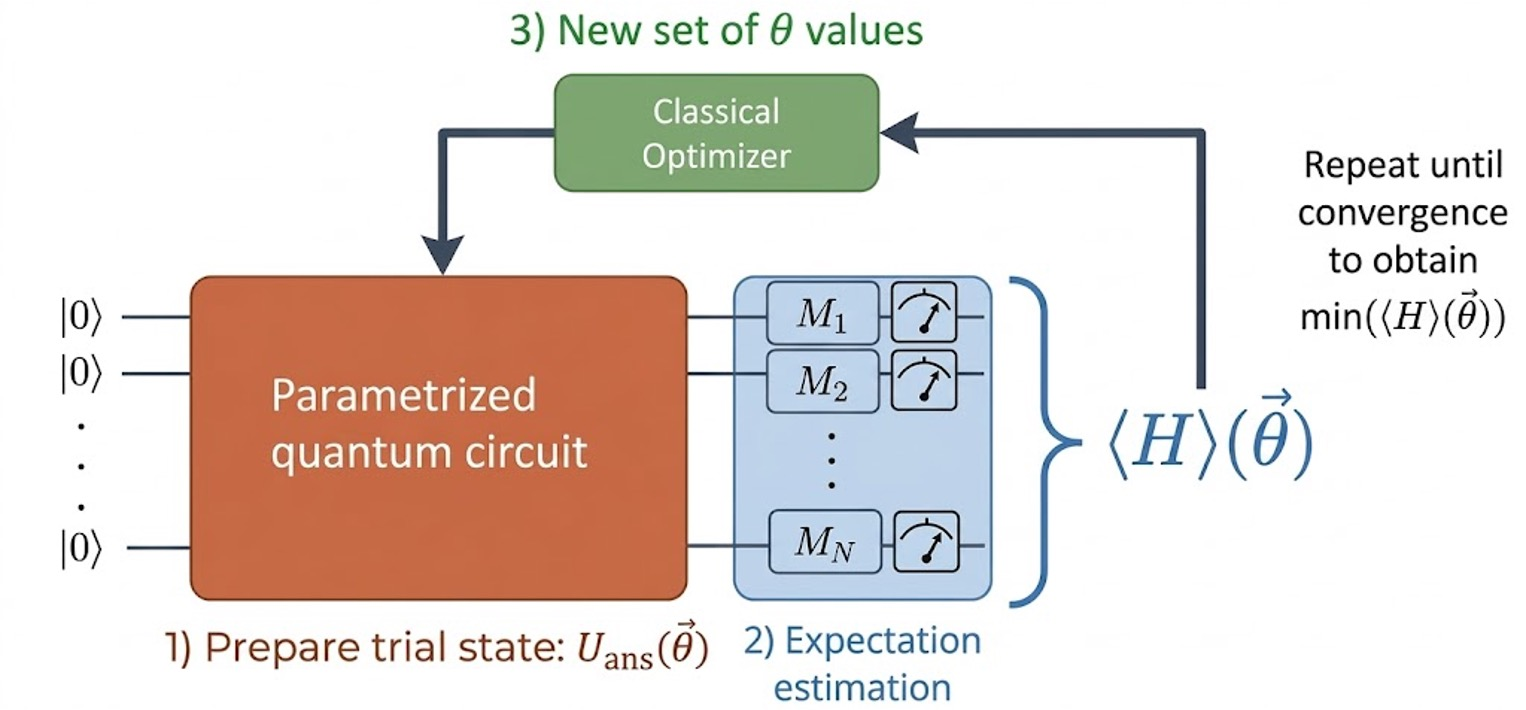
\includegraphics[width=0.8\linewidth]{General_Sections/Figures/vqe_demonstration.jpg}
    \caption{Schematic representation of the VQE hybrid architecture. The process illustrates the iterative feedback loop between the QPU, responsible for state preparation and measurement, and the CPU, which executes the optimization algorithm to update the variational parameters $\boldsymbol{\theta}$.}
    \label{fig:VQE_loop}
\end{figure}

\subsection{Combinatorial optimization on quantum devices}
While variational methods such as VQE are naturally formulated as energy-minimization problems over quantum states, many problems in computational biology involve discrete decision variables. Sequence design is one such example: at each position, a finite set of amino-acid identities must be selected, resulting in a combinatorial search space whose size grows exponentially with peptide length. Quantum optimization algorithms can address such problems by encoding the discrete variables into qubits and expressing the corresponding objective function as a cost Hamiltonian.
\subsubsection{Quadratic Unconstrained Binary Optimization (QUBO)}
The sequence-design problems considered in this research are formulated as Quadratic Unconstrained Binary Optimization (QUBO) problems~\cite{qubo_2}. A QUBO consists of minimizing a quadratic function of binary variables $x_i\in\{0,1\}$:
\begin{equation}
\min_{\mathbf{x}\in\{0,1\}^n} \quad \sum_i c_i x_i
+
\sum_{i<j}Q_{ij}x_ix_j
\end{equation}
where $c_i$ are the linear coefficients and $Q_{ij}$ describe pairwise interactions between binary variables. In the context of sequence design, these coefficients can encode contributions associated with individual amino-acid choices and pairwise interactions between selected residues.
QUBO formulations can be mapped to Ising Hamiltonians by introducing a binary-to-spin transformation. Using:
\begin{equation}
x_i=\frac{1-Z_i}{2}
\end{equation}
where $Z_i$ denotes the Pauli-$Z$ operator acting on qubit $i$, the QUBO objective can be transformed into a diagonal Hamiltonian of the form:
\begin{equation}
\hat{H}_C = K
+
\sum_i h_i Z_i
+
\sum_{i<j}J_{ij}Z_iZ_j
\end{equation}
where $K$, $h_i$, and $J_{ij}$ are the coefficients resulting from the binary-to-spin transformation. Because this Hamiltonian is diagonal in the computational basis, each binary configuration $\mathbf{x}$ corresponds to a computational-basis state $|\mathbf{x}\rangle$, and the corresponding eigenvalue reproduces the value of the original QUBO objective up to an additive constant. Since this constant does not affect the location of the minimum, the minimum-energy computational-basis state represents the optimal solution of the corresponding QUBO problem~\cite{qubo_1}.


\paragraph{Handling constraints via penalty terms}
Biological sequence-design problems are often subject to constraints, for example requiring a fixed number of selected residues, limiting the number of mutations, or enforcing a prescribed net charge. In a QUBO formulation, such constraints can be incorporated into the objective through penalty terms. For a set of linear constraints of the form:
\begin{equation}
A\mathbf{x}=\mathbf{b}
\end{equation}
a corresponding penalized objective can be written as:
\begin{equation}
f_{\mathrm{penalized}}(\mathbf{x}) = f(\mathbf{x})
+
\lambda
\left\|
A\mathbf{x}-\mathbf{b}
\right\|_2^2
\end{equation}
where $\lambda>0$ controls the energetic cost associated with constraint violations~\cite{qubo_2}. For binary variables, the identity $x_i^2=x_i$ ensures that expanding the quadratic penalty does not introduce terms of order higher than two. The resulting objective therefore remains within the QUBO form. The penalty coefficient must be chosen sufficiently large to discourage invalid configurations without unnecessarily dominating the original optimization objective.




\subsubsection{The Quantum Approximate Optimization Algorithm}
Once a discrete optimization problem has been expressed as a cost Hamiltonian $\hat{H}_C$, the QAOA can be used to search for low-energy computational-basis states. QAOA was introduced by Farhi, Goldstone, and Gutmann as a variational quantum algorithm for approximate combinatorial optimization~\cite{QAOA}. It constructs a parameterized quantum state by alternating the action of a cost Hamiltonian and a mixing Hamiltonian. The corresponding variational parameters are optimized classically using measurements obtained from the quantum circuit.
\paragraph{Connection with adiabatic quantum optimization}
The construction of QAOA is closely related to the principles of adiabatic quantum optimization. In the adiabatic approach, a quantum system is initialized in the ground state of an easily prepared Hamiltonian $\hat{H}_B$ and subsequently evolved according to a time-dependent Hamiltonian,
\begin{equation}
\hat{H}(t) = [1-s(t)]\hat{H}_B
+
s(t)\hat{H}_C
\end{equation}
where the schedule $s(t)$ varies continuously from $s(0)=0$ to $s(T)=1$. A commonly used initial or driver Hamiltonian is:
\begin{equation}
\hat{H}_M = -\sum_{i=1}^{N}X_i
\end{equation}
where $X_i$ denotes the Pauli-$X$ operator acting on qubit $i$. Its ground state is the uniform superposition:
\begin{equation}
|+\rangle^{\otimes N} = \left(\frac{|0\rangle+|1\rangle}{\sqrt{2}}\right)^{\otimes N}
\end{equation}
The cost Hamiltonian $\hat{H}_C$ encodes the classical optimization problem. Under ideal adiabatic evolution, the system remains close to the instantaneous ground state if the evolution is sufficiently slow relative to the relevant spectral gap and the rate at which the Hamiltonian changes~\cite{nielsen2010quantum}. The computational resources required to satisfy this condition depend strongly on the minimum spectral gap encountered along the chosen evolution path. For difficult optimization problems, this gap can become very small, potentially leading to evolution times that are impractical for near-term devices.
QAOA can be viewed as a variational, gate-based formulation motivated by this continuous evolution. Instead of following a prescribed continuous schedule, the evolution is replaced by an alternating sequence of cost and mixing unitaries. For a circuit with $p$ layers, the QAOA unitary can be written as:
\begin{equation}
\hat{U}(\boldsymbol{\gamma},\boldsymbol{\beta}) = \prod_{k=1}^{p}
e^{-i\beta_k\hat{H}_M}
e^{-i\gamma_k\hat{H}_C}
\end{equation}
where $\hat{H}_M$ denotes the mixing Hamiltonian, $\boldsymbol{\gamma}=(\gamma_1,\ldots,\gamma_p)$ and $\boldsymbol{\beta}=(\beta_1,\ldots,\beta_p)$ are independent sets of variational parameters, and $p$ determines the number of alternating layers. For the standard mixer $\hat{H}_M=-\sum_iX_i$, the initial state is chosen as the ground state of $\hat{H}_M$:
\begin{equation}
|\psi_p(\boldsymbol{\gamma},\boldsymbol{\beta})\rangle = \hat{U}(\boldsymbol{\gamma},\boldsymbol{\beta})
|+\rangle^{\otimes N}
\end{equation}
The connection with adiabatic evolution can be motivated by a Trotter-like discretization of the continuous evolution. However, QAOA is not simply a finite-step approximation of a fixed adiabatic schedule. The parameters $\boldsymbol{\gamma}$ and $\boldsymbol{\beta}$ are treated as free variational parameters and are optimized directly for the problem at hand. Increasing $p$ enlarges the variational flexibility of the circuit, but also increases its depth, number of operations, and susceptibility to hardware noise.
The QAOA objective function is given by the expectation value of the cost Hamiltonian,
\begin{equation}
F_p(\boldsymbol{\gamma},\boldsymbol{\beta}) = \langle
\psi_p(\boldsymbol{\gamma},\boldsymbol{\beta})
|
\hat{H}_C
|
\psi_p(\boldsymbol{\gamma},\boldsymbol{\beta})
\rangle
\end{equation}
The parameters are optimized iteratively using a classical optimizer. At each iteration, the QPU prepares the QAOA state and performs the measurements required to estimate the expectation value of the cost Hamiltonian. The classical optimizer then uses the resulting estimate of $F_p$ to determine updated values of $\boldsymbol{\gamma}$ and $\boldsymbol{\beta}$. At finite circuit depth, the variational optimization is not guaranteed to recover the global optimum, and the final result depends on the circuit depth, parameter initialization, optimization strategy, measurement uncertainty, and hardware noise.
A standard benchmark for QAOA is the MaxCut problem, which admits a direct mapping to an Ising cost Hamiltonian~\cite{max_cut_np_hard}. In this thesis, QAOA is instead applied to a peptide sequence-design problem, in which binary variables encode discrete amino-acid choices and the cost Hamiltonian represents an environment-dependent objective. This formulation allows the quantum circuit to act as a heuristic search procedure over a discrete sequence space while retaining an explicit energy-based representation of the optimization objective.


\begin{figure}[!htbp]
    \centering
    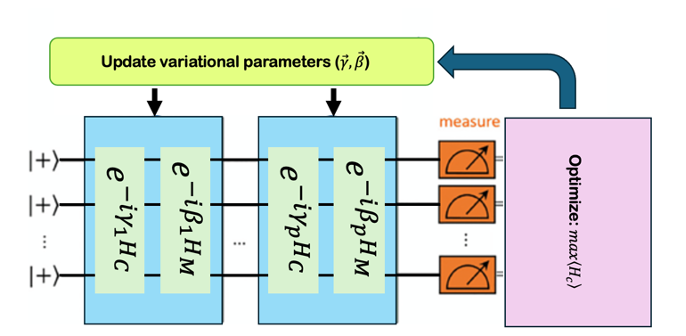
\includegraphics[width=0.8\linewidth]{General_Sections/Figures/qaoa_demonstration.png}
    \caption{Schematic representation of the QAOA circuit architecture for a depth $p$. The circuit begins with a layer of Hadamard gates to create a uniform superposition $|+\rangle^{\otimes N}$, followed by alternating layers of the cost unitary $e^{-i\gamma_k \hat{H}_C}$ and the mixer unitary $e^{-i\beta_k \hat{H}_B}$. Finally, the state is measured in the computational basis.}
    \label{fig:QAOA_circ}
\end{figure}

\paragraph{Conditional Value at Risk (CVaR) optimization}
In addition to the standard expectation-value objective, the QAOA optimization considered in this work employs the CVaR as an alternative objective function~\cite{cvar_1}. Whereas the expectation value incorporates all possible measurement outcomes according to their sampling probabilities, CVaR focuses specifically on the lower-energy tail of the sampled distribution. This provides a mechanism for directing the classical optimization towards regions of the parameter space that yield a higher probability of observing low-energy solutions.
For a confidence level $\alpha\in(0,1]$ and a fixed measurement budget of $K$ shots, let the measured energies be sorted in ascending order,
\begin{equation}
e_1 \leq e_2 \leq \dots \leq e_K
\end{equation}
The empirical CVaR estimator used in this work is defined as the mean energy of the lowest-energy fraction of the measured outcomes:
\begin{equation}
\mathrm{CVaR}_{\alpha} = \frac{1}{\lceil\alpha K\rceil}
\sum_{k=1}^{\lceil\alpha K\rceil} e_k
\end{equation}
Here, $\alpha=1$ corresponds to the mean energy over all measured outcomes, recovering the standard sample-mean objective. In contrast, smaller values of $\alpha$ progressively restrict the estimator to the lowest-energy outcomes. For example, $\alpha=0.1$ considers the lowest-energy $10\%$ of the measured samples. In the limit of small $\alpha$, the objective increasingly emphasizes the best observed outcomes, although it remains an estimator based on a finite number of measurements and therefore does not necessarily identify the true global optimum.
In this work, CVaR is used as an alternative objective function for the classical optimization of the QAOA parameters, rather than as a modification of the underlying quantum circuit. The QAOA state preparation and measurement procedure therefore remain unchanged; only the way in which the measured computational-basis outcomes are aggregated into the classical objective is modified.
The choice of $\alpha$ introduces a trade-off between the statistical information retained from the measurement distribution and the emphasis placed on low-energy outcomes. Decreasing $\alpha$ increases the focus on the lower-energy tail but reduces the number of samples contributing to the estimator, potentially increasing its statistical uncertainty for a fixed shot budget. Consequently, very small values of $\alpha$ may make the optimization more sensitive to sampling fluctuations. CVaR does not, by itself, eliminate hardware noise or measurement errors. Comparisons between CVaR and expectation-value optimization should therefore be performed using the same measurement budget and otherwise equivalent experimental conditions~\cite{cvar_1,cvar_2}.

\subsection{Classical optimization in hybrid workflows}
Variational quantum algorithms rely on a classical optimization procedure to update the parameters of the quantum circuit. The resulting objective landscape can be non-convex, while finite-shot measurements introduce statistical fluctuations and hardware noise can further perturb the objective evaluations. The choice of classical optimizer therefore constitutes an additional component of the computational workflow.
In this work, several derivative-free optimization approaches were explored during the development of the variational workflows. These methods do not require explicit gradient evaluation and can operate directly on objective functions affected by finite-shot sampling and hardware noise. Among the approaches considered were COBYLA, which provides a local model-based optimization strategy, and Differential Evolution (DE), a population-based stochastic optimization method~\cite{Failde2023,Kandala2017,DE,DE_2}.



\subsubsection{Constrained Optimization BY Linear Approximations}
Constrained Optimization BY Linear Approximations is a derivative-free, model-based optimization algorithm originally developed by M.~J.~D.~Powell for nonlinear constrained optimization~\cite{COBYLA}. At each iteration, COBYLA constructs local linear approximations of the objective function and constraints using function evaluations at a set of nearby points. These approximations are then optimized within a local region around the current solution.
For an $n$-dimensional parameter vector $\vec{x}$, the local subproblem can be expressed schematically as:
\begin{equation}
\begin{aligned}
\min_{\vec{x}\in\mathbb{R}^n}
\quad &
\hat{f}_k(\vec{x}) \\
\text{s.t.}\quad &
\hat{c}_{k,i}(\vec{x})\leq 0,
\quad i\in I,\\
&
\|\vec{x}-\vec{x}_k\|\leq\Delta_k,
\end{aligned}
\end{equation}
where $\hat{f}_k$ and $\hat{c}_{k,i}$ denote local linear approximations of the objective and constraint functions, respectively, $\vec{x}_k$ is the current iterate, and $\Delta_k$ defines the size of the local optimization region. Restricting the optimization to this region limits the step to a domain in which the linear approximations are expected to provide a useful description of the objective and constraints. The size of this region is subsequently adjusted according to the progress of the optimization.
For the variational circuits considered in this work, the optimization variables $\vec{x}$ correspond to the circuit parameters, such as rotation angles. Since COBYLA does not require analytical or quantum-measured gradients, it can be applied directly to objective functions obtained from finite-shot quantum measurements. This makes it suitable for hybrid quantum--classical workflows in which objective evaluations may be noisy or computationally expensive.
\subsubsection{Differential Evolution}
DE is a stochastic, population-based optimization algorithm introduced by Storn and Price for the global optimization of continuous parameter spaces~\cite{DE,DE_2}. Unlike local model-based methods, DE maintains a population of candidate solutions and generates new candidates using scaled differences between population members. This population-based strategy can promote exploration of different regions of a multimodal objective landscape without requiring gradient information.
At generation $g$, the population consists of $NP$ parameter vectors $\vec{x}_{i,g}$. The evolutionary process is based on three main operations:
\begin{itemize}
\item \textbf{Mutation:} A mutant vector is generated from a base population vector and a scaled difference between two other population members. For the commonly used DE/rand/1 strategy,
\begin{equation}
\vec{v}_{i,g} = \vec{x}_{r_1,g} + F\left(\vec{x}_{r_2,g} - \vec{x}_{r_3,g}\right)
\end{equation}
where $r_1$, $r_2$, and $r_3$ are distinct randomly selected indices and $F$ is the differential-weight parameter.
\item \textbf{Crossover:} The mutant vector is combined with the target vector $\vec{x}_{i,g}$ to generate a trial vector $\vec{u}_{i,g}$. For binomial crossover, each component is selected from the mutant vector with probability $C_r$, while the remaining components are inherited from the target vector. At least one component is typically forced to originate from the mutant vector to ensure that the trial vector differs from the target vector.
\item \textbf{Selection:} The trial vector is compared with its corresponding target vector according to the objective function. For a minimization problem, the candidate yielding the lower objective value is retained for the next generation.
\end{itemize}
The population-based nature of DE allows multiple candidate solutions to be explored simultaneously and does not rely on local gradient information. However, DE remains a stochastic heuristic and does not guarantee convergence to the global optimum. Its behavior can depend on factors including the population size, mutation strategy, crossover probability, parameter bounds, and the statistical noise associated with the objective-function evaluations.










\subsection{Challenges and noise mitigation in the NISQ era}
The implementation of quantum algorithms on current hardware is constrained by several sources of physical and operational noise. These limitations affect both the preparation of quantum states and the measurement of observables and therefore need to be considered when interpreting results obtained from NISQ devices.
\subsubsection{Decoherence and gate errors}
A fundamental limitation of quantum processors is the interaction of qubits with their surrounding environment, which leads to decoherence and the gradual loss of quantum information over time~\cite{nielsen2010quantum}. Two characteristic timescales are commonly used to describe this behavior: the relaxation time $T_1$, which characterizes the decay of excited-state populations towards the ground state, and the dephasing time $T_2$, which characterizes the decay of phase coherence between quantum states~\cite{error_mitigation_1}.
In addition to decoherence, quantum operations and measurements are affected by control and readout errors. These can arise from imperfect control pulses, unwanted interactions between qubits, fluctuations in the physical environment, and other hardware-dependent effects. As a result, the output of a quantum circuit generally deviates from the ideal evolution predicted by its theoretical description. The impact of these errors tends to increase with circuit depth, although their effect on a particular calculation depends on factors including the error rates, circuit architecture, qubit connectivity, coherence times, and the observable being measured~\cite{nielsen2010quantum}.
\subsubsection{Quantum Error Mitigation (QEM)}
Unlike quantum error correction, which aims to encode logical qubits into larger sets of physical qubits and actively suppress errors during computation, Quantum Error Mitigation (QEM) seeks to reduce the effect of noise on measured observables through modified circuit executions and classical post-processing~\cite{error_mitigation_2}. QEM is therefore particularly relevant to NISQ devices, where full fault-tolerant quantum error correction remains impractical for large-scale applications.
Several error-mitigation strategies have been developed, including:
\begin{itemize}
\item \textbf{Zero-noise extrapolation (ZNE):} The effective noise affecting a circuit is intentionally increased, for example through gate folding or other noise-scaling procedures, and the corresponding expectation values are measured at several effective noise levels. These values are then extrapolated towards the zero-noise limit~\cite{error_mitigation_3}. The method does not physically remove noise from the circuit; instead, it attempts to estimate the observable that would have been obtained in the absence of noise.
\item \textbf{Measurement error mitigation:} Errors occurring during the readout process can lead to incorrect assignment of qubit states. Measurement error mitigation characterizes these assignment probabilities through calibration experiments and uses the resulting calibration information to correct the measured probability distribution or expectation values~\cite{error_mitigation_4}. Because such corrections can involve matrix inversion or related statistical procedures, they may amplify statistical fluctuations and increase the variance of the resulting estimator.
\item \textbf{Probabilistic error cancellation (PEC):} PEC represents an ideal noise-free operation as a linear combination of noisy operations that can be implemented experimentally. The resulting quasi-probability representation is sampled through repeated circuit executions, and the measurements are combined with the corresponding quasi-probability weights to construct an estimator of the ideal observable~\cite{error_mitigation_3}. Although PEC can, under appropriate assumptions, reduce systematic noise bias, its sampling overhead can increase substantially with circuit depth and noise strength.
\end{itemize}
These techniques illustrate an important trade-off in NISQ computation: reducing systematic errors generally introduces additional computational and statistical overhead. Consequently, error mitigation does not provide a free correction of noisy quantum calculations, but instead trades additional measurements and classical processing for a potentially reduced bias in the estimated observables.
In the context of this thesis, error-mitigation techniques are considered as part of the classical post-processing and optimization workflow when applicable to the quantum hardware and computational experiment. Their use must therefore be interpreted together with the associated measurement overhead, statistical uncertainty, and hardware-specific noise characteristics.

% Results and Discussion
\chapter{Results: Published Articles}
\chapterquote{Always pass on what you have learned.}{Yoda, Episode VIII}
\newpage

%% Section 1
\fakesection{Cain Triangle}\label{chap1}
\newpage

\subsection{Unraveling lipid and inflammation interplay in cancer, aging and infection for novel theranostic approaches}\label{art:lipids_review}
% \noindent
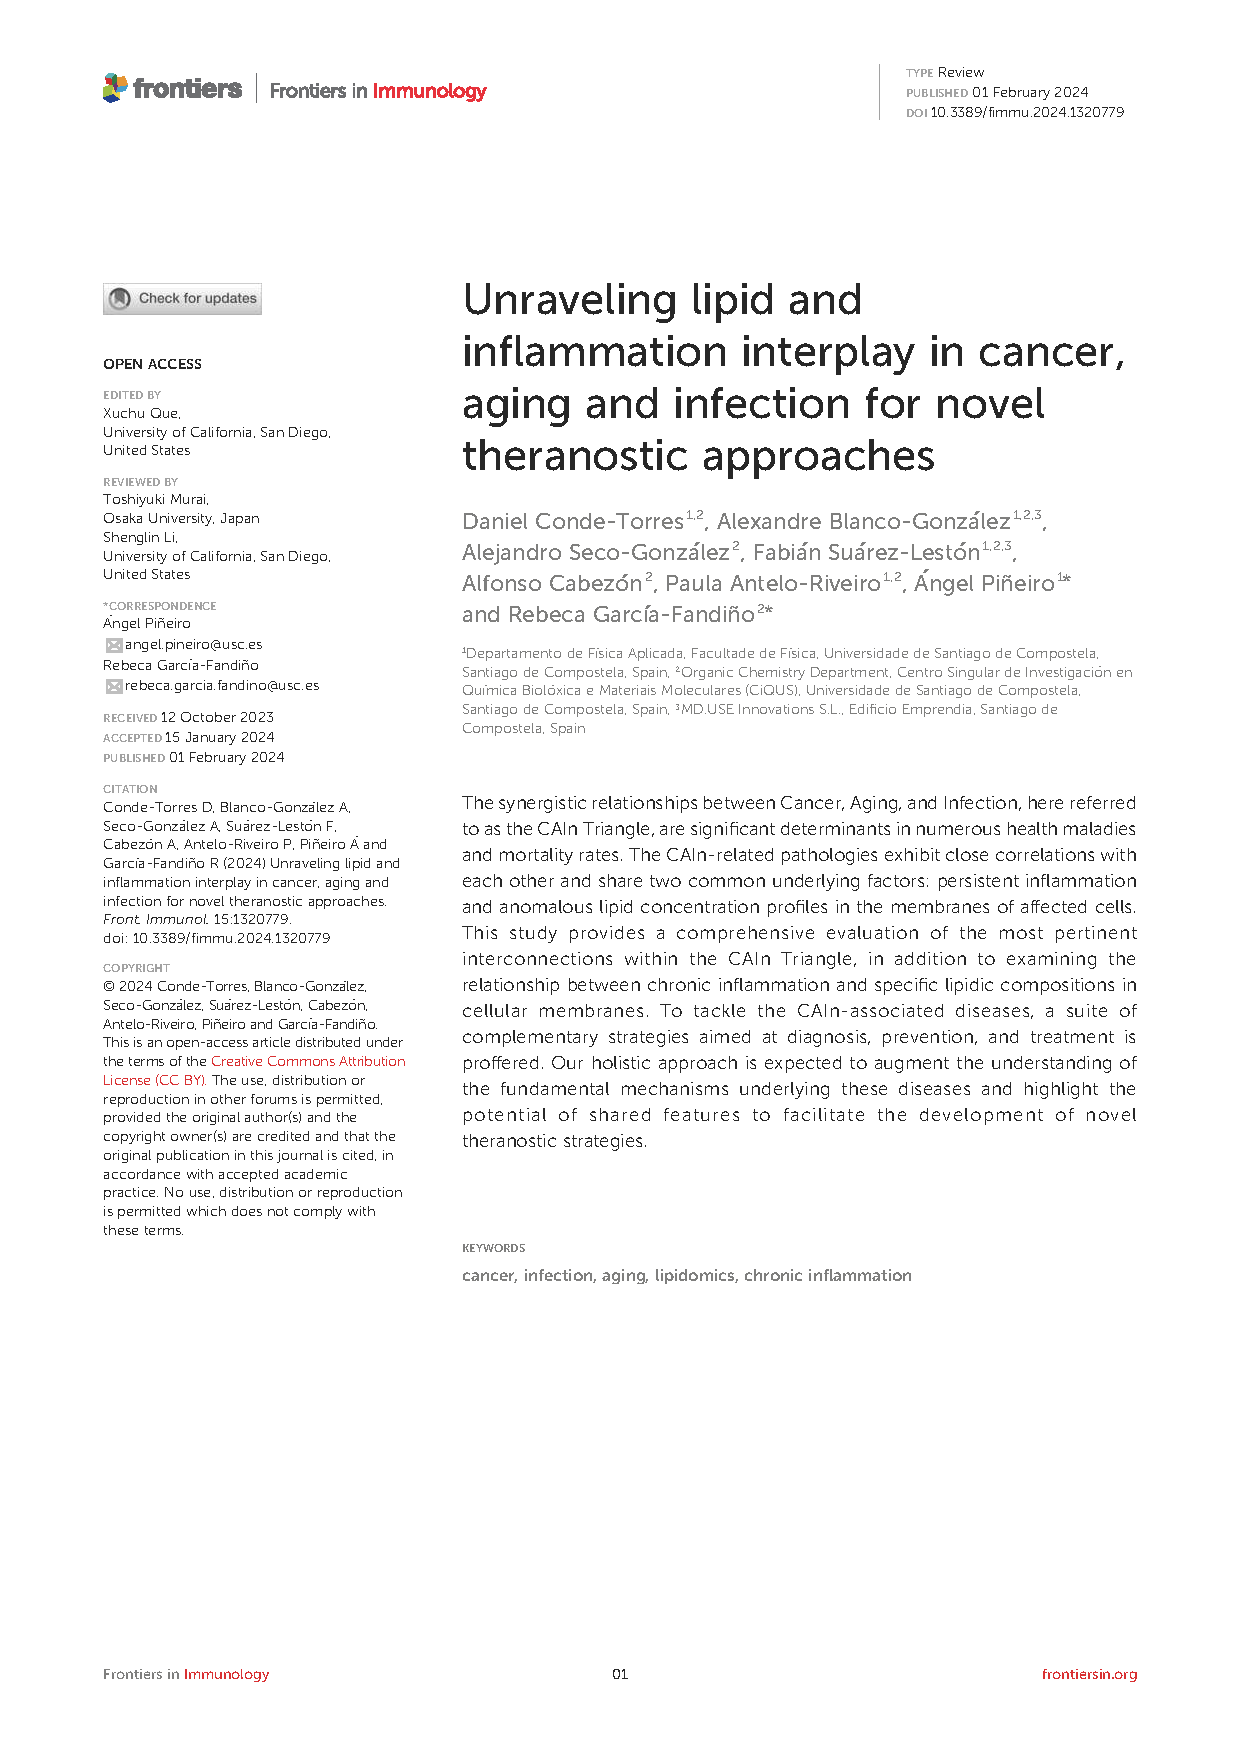
\includegraphics[page=1, width = 1.06\linewidth]{Results_Discussion/Papers/Papers_principales/Introduction_lipids_compressed.pdf}


\includepdf[pages=2-, width = 1.15\linewidth, pagecommand={\thispagestyle{fancy}}]{Results_Discussion/Papers/Papers_principales/Introduction_lipids_compressed.pdf}

%% Section 2
\fakesection{Metadynamics}\label{chap2}
\newpage

\subsection{Unlocking the specificity of antimicrobial peptide interactions for membrane-targeted therapies}\label{art:metadynamics}

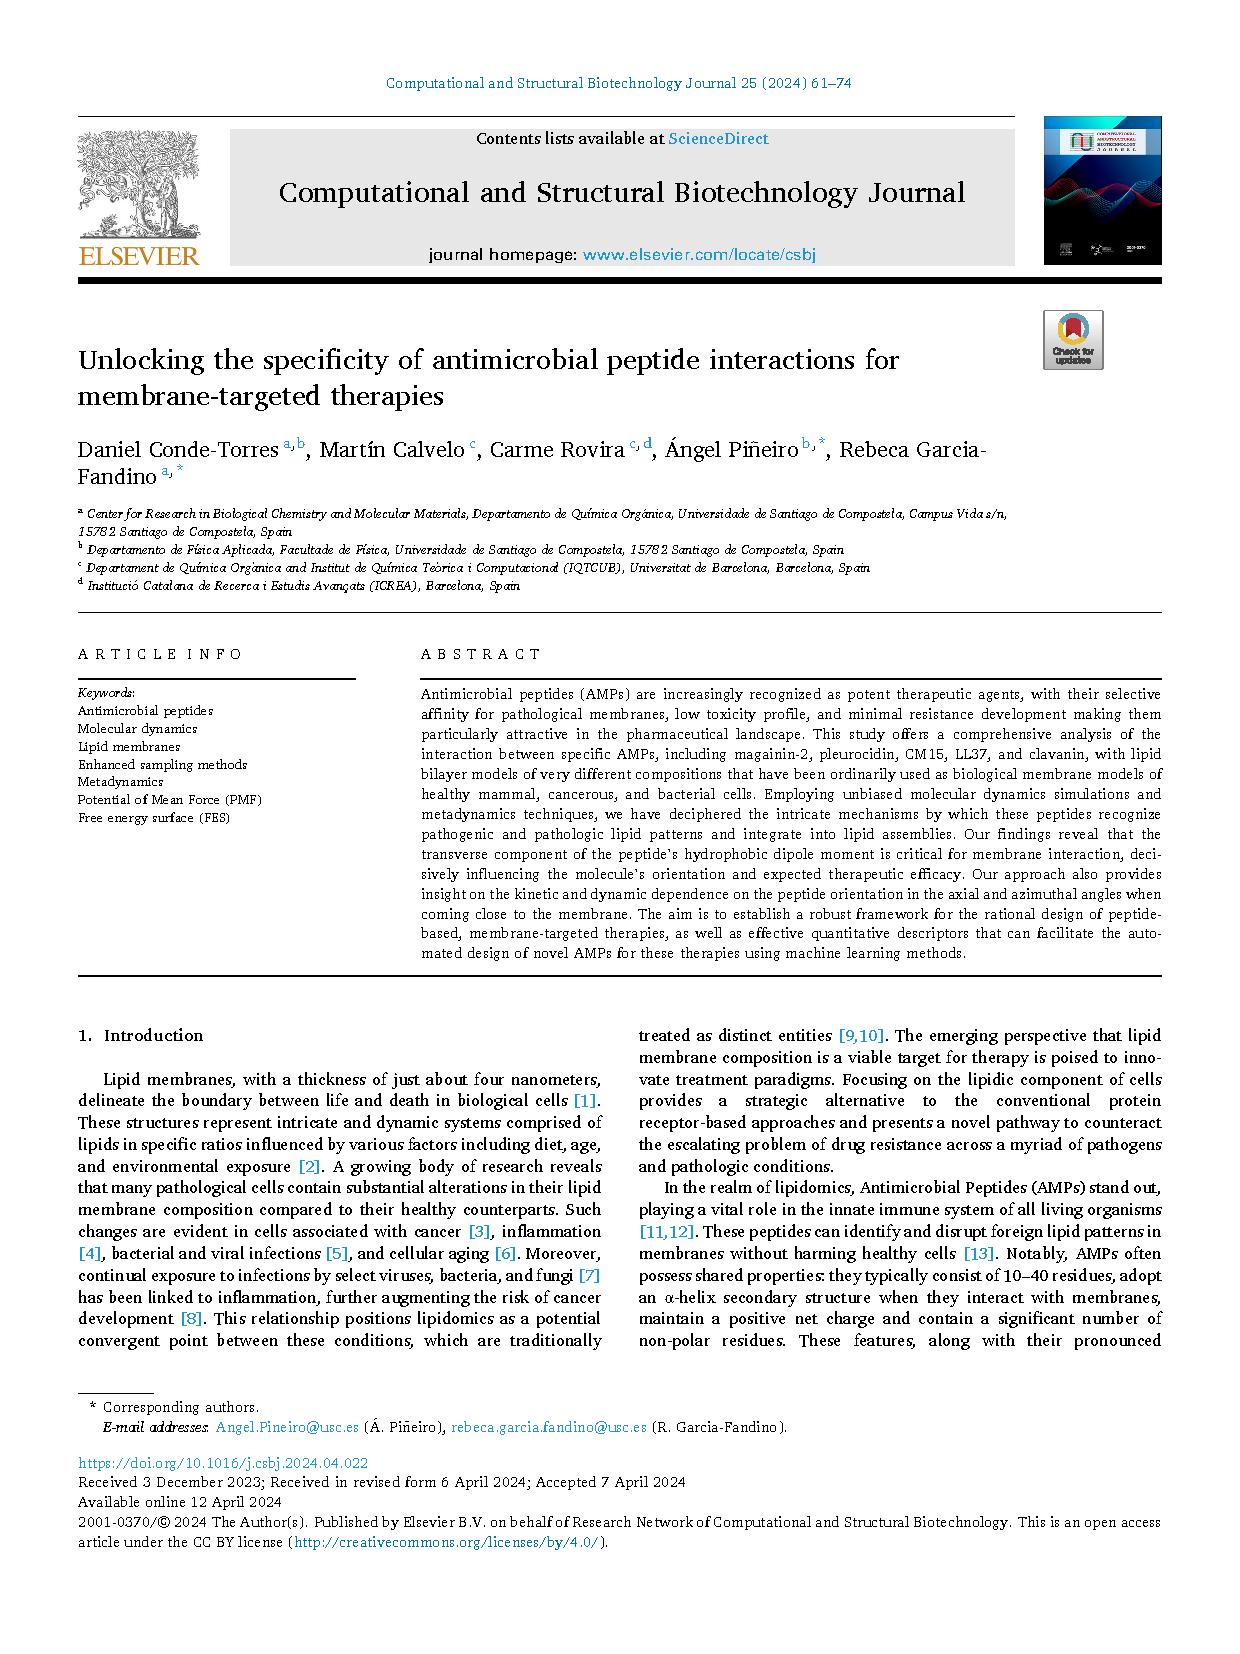
\includegraphics[page=1, width = \linewidth]{Results_Discussion/Papers/Papers_principales/metadinamica.pdf}


\includepdf[pages=2-, width = 1.2\linewidth, pagecommand={\thispagestyle{fancy}}]{Results_Discussion/Papers/Papers_principales/metadinamica.pdf}

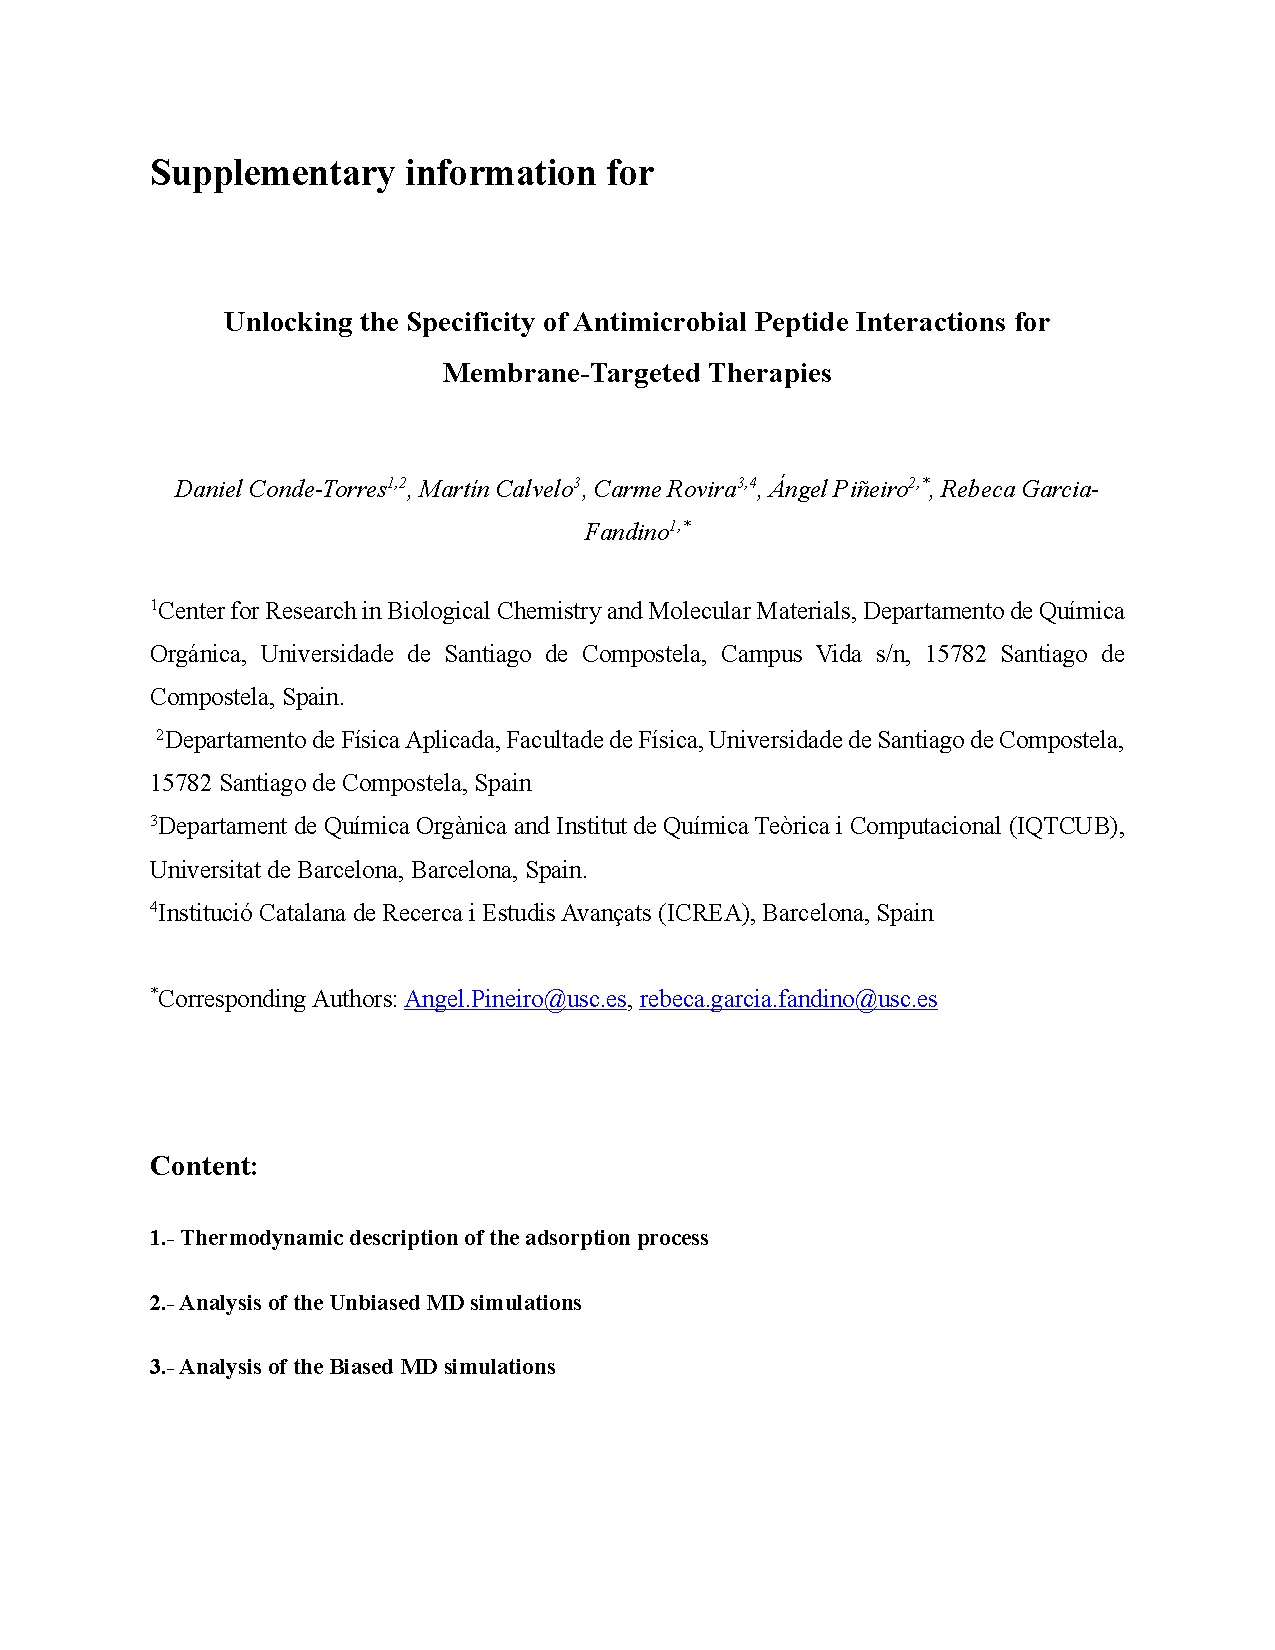
\includepdf[pages=1-, width = 1.2\linewidth, pagecommand={\thispagestyle{fancy}}]{Results_Discussion/Papers/Papers_principales/metadinamica_SI.pdf}


\subsection{Classical Simulations on Quantum Computers: Interface-Driven Peptide Folding on Simulated Membrane Surfaces}\label{art:vqe_cesga}

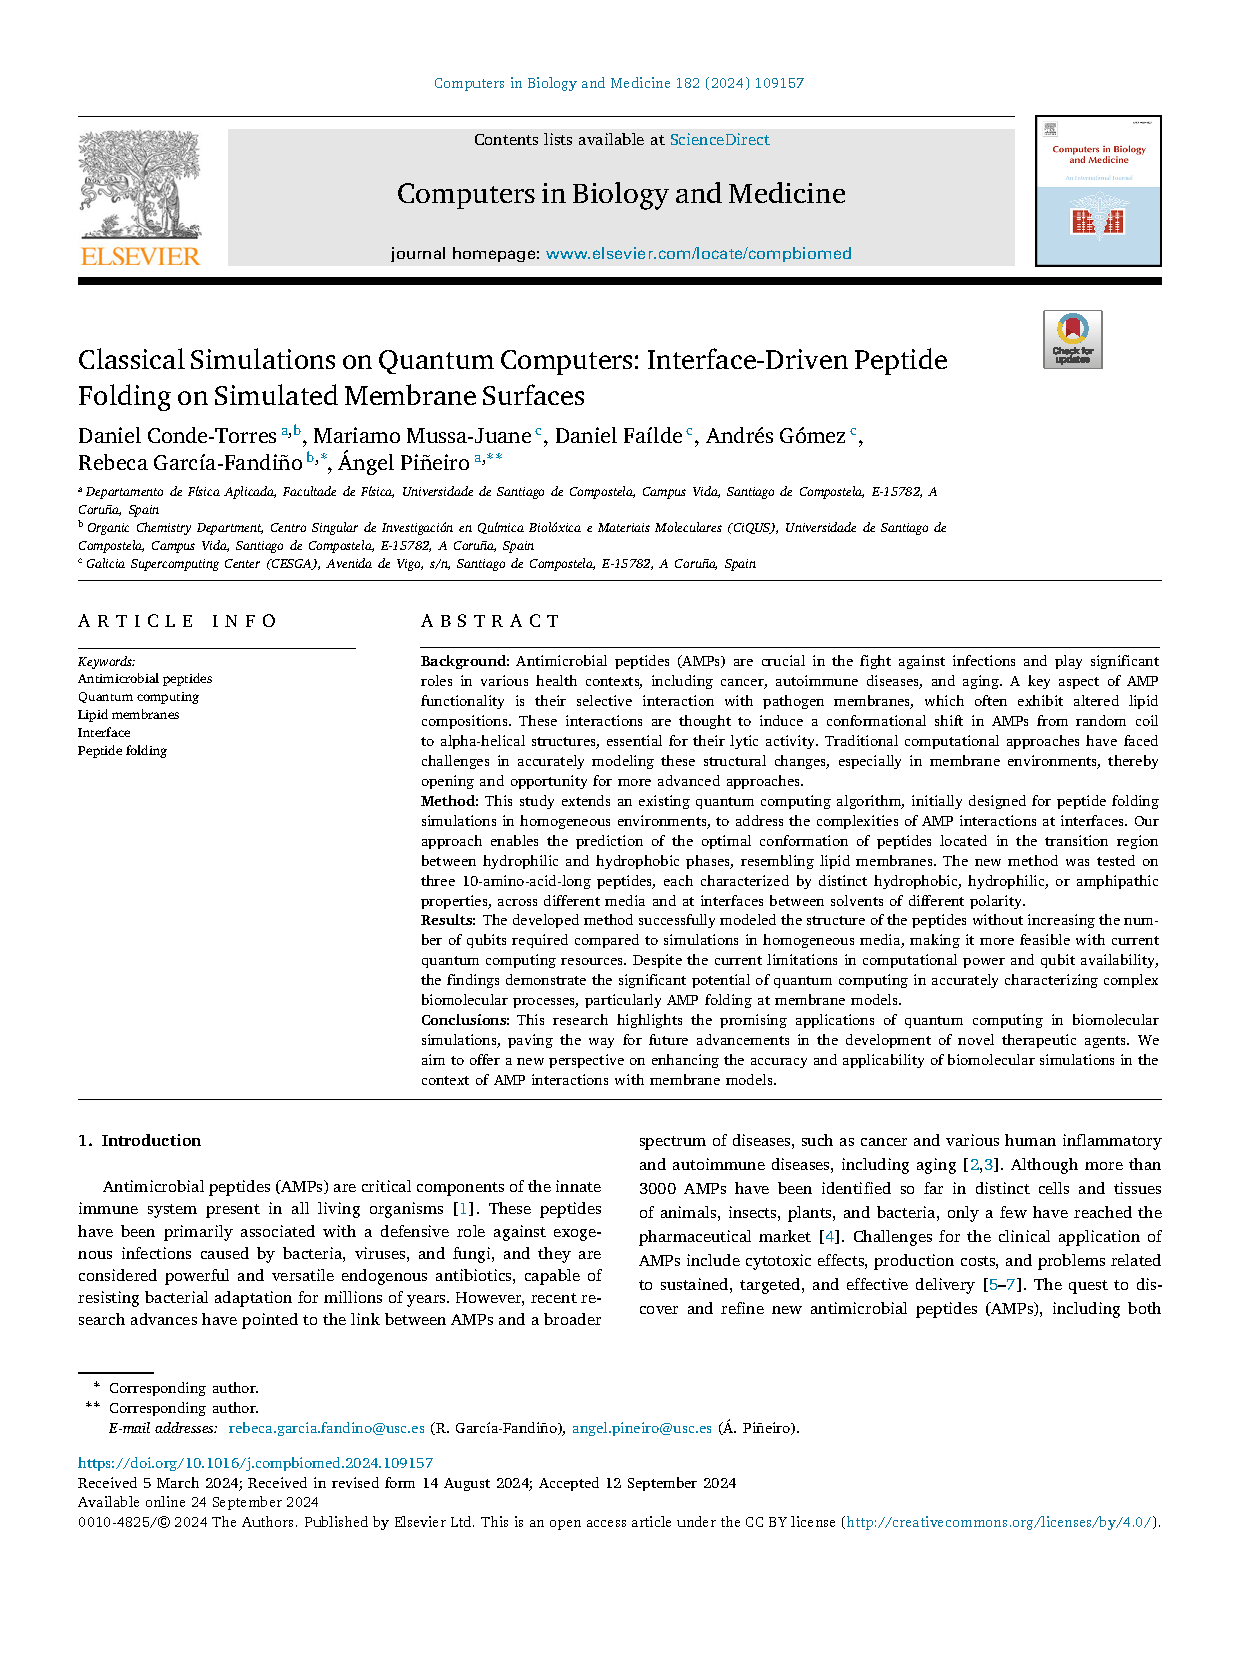
\includegraphics[page=1, width = \linewidth]{Results_Discussion/Papers/Papers_principales/vqe_cesga.pdf}


\includepdf[pages=2-, width = 1.15\linewidth, pagecommand={\thispagestyle{fancy}}]{Results_Discussion/Papers/Papers_principales/vqe_cesga.pdf}
\hypertarget{registro}{}

%% Section 2
% \fakesection{Creating a Database of Cyclic Peptide Molecular Dynamics Results}\label{chap2}
% \chapterquote{GROMACS reminds you: ` `I am rarely happier than when spending an entire day programming my computer to perform automatically a task that it would otherwise take me a good ten seconds to do by hand." (Douglas Adams)}

% \newpage

% \subsection{CYCLOPEpDB: Bridging Molecular Dynamics Simulations and Machine Learning for Predicting Cyclic Peptide-Membrane Interactions.}\label{art:CPDB}



% Unpublished Results
\chapter{Unpublished results}\label{chap:unpublished}
\chapterquote{Perhaps the archives are incomplete.}{Obi-Wan Kenobi, Star Wars: Episode II}

%% Section 1
\fakesection{Environment-conditioned design: A physics-based hamiltonian pivot}\label{chap3}
\newpage

\subsection{Environment-conditioned design of $\alpha$-helical peptides}\label{art:hamiltonian}


\includegraphics[page=1, width=0.9\linewidth]{Results_Discussion/Papers/Papers_secundarios/hamiltonian_design.pdf}


\includepdf[pages=2-, width=1.1\linewidth, offset=0cm -1cm, pagecommand={\thispagestyle{fancy}}]{Results_Discussion/Papers/Papers_secundarios/hamiltonian_design.pdf}


\includepdf[pages=1-, width=1.1\linewidth, offset=0cm -1cm, pagecommand={\thispagestyle{fancy}}]{Results_Discussion/Papers/Papers_secundarios/hamiltonian_design_si.pdf}

\subsection{Helix Design Studio: A Web Platform for Environment-Conditioned Design of $\alpha$-Helical Peptides}\label{art:web_page}


\includegraphics[page=1, width=1.1\linewidth]{Results_Discussion/Papers/Papers_secundarios/bibliometria.pdf}


\includepdf[pages=2-, width=1.1\linewidth, offset=0cm -1cm, pagecommand={\thispagestyle{fancy}}]{Results_Discussion/Papers/Papers_secundarios/bibliometria.pdf}


%General Discussion
\chapter{General Discussion}\label{discussion}
\chapterquote{GROMACS reminds you: “All models are wrong, but some are useful.” (George Box)}

\newpage

Modern biomedicine faces a major challenge as antimicrobial resistance keeps rising. To counter this threat, novel antimicrobial drugs that eliminate pathogens through alternative mechanisms are urgently required. In this regard, membrane-targeted antimicrobial peptides are highly promising scaffolds capable of exhibiting antimicrobial activity by targeting lipidic membranes, However, their therapeutic promise is often capped by their low stability in biological media. Linear antimicrobial peptides are particularly susceptible to proteolytic degradation, typically displaying short circulation half-lives, and may present toxicity toward host cells, which together hinder their clinical translation. Cyclic peptides stand out as a compelling answer. Cyclization constrains the backbone, often improving proteolytic stability and pharmacokinetics. Among cyclic peptides, those formed by alternation of D,L-\(\alpha\)-amino acids attracted much attention as they can stack into ordered nanotubes exhibiting functions such as ion transport or membrane disruption. Nonetheless, their self-assembly and membrane interactions depend sensitively on the amino acid composition. Since small changes in amino acid composition can completely modify the behavior of the cyclic peptide in the presence of lipidic membranes, understanding and designing that behavior calls for a lens that can resolve dynamics at the atomic level.

Experimentally, using wet-lab experimental assays, these questions are challenging to address. Experiments assessing peptide-membrane interactions often differ in protocol and readout, making the formulation of coherent sequence–function rules across heterogeneous datasets nontrivial. Even when high-quality measurements are available, the intrinsic lack of atomic resolution, leads to the condensation of complex dynamic processes into single scalar endpoints that represent membrane interaction. Molecular dynamics simulations, at all-atom resolution can capture cyclic peptide-membrane interaction insights with atomic detail. However, the time and length scales relevant to study these systems at such level of resolution are computationally demanding. Coarse-grained models address this limitation by grouping atoms into interaction centers, sacrificing some chemical detail in exchange of more sampling capabilities. For peptides and membranes, the MARTINI family of models has become widely used. A key limitation arises here: in standard Martini, the peptide backbone is represented by a single interaction center, loosing then the directionality of CPs by not considering the amide N–H and C=O groups that govern their assembly. In practice, this leads to unrealistic rotational angles between cyclic peptide rings and indistinguishable parallel and antiparallel stacking, thus biasing aggregation propensity. In short, without careful adaptation, access to longer time scales may come at the expense of capturing the essential physics of CPs.

At the same time, data-driven methods have matured to the point where predicting peptide properties or functions from amino acid sequences has become routine in many areas of molecular design. The limiting factor is no longer algorithmic complexity but data quality. Experimental data obtained from wet-lab assays, although invaluable, is often highly heterogeneous, as it combines results from different assays, protocols, and literature sources. This heterogeneity complicates the extraction of consistent sequence–function relationships. In contrast, MD simulations provide a controlled and reproducible framework in which thousands of \textit{in-silico} experiments can be performed under homogeneous conditions. MD trajectories yield rich, three dimensional, and time-resolved information, from which physically meaningful descriptors can be systematically extracted at atomic or near-atomic precision. Such data is particularly well suited for training machine learning models, enabling them to learn structure-dynamics-function relationships and to generalize reliably to previously unseen sequences.

This thesis embraces this synergy between MD and ML and develops it through three connected steps, presented in four published articles and a yet unpublished manuscript. First, across two publications, the MARTINI force field was adapted by introducing a chirality-aware coarse-grained representation of CPs that restores the hydrogen-bond directionality required to reproduce realistic self-assembly interactions. Moreover, in a third work, that representation was made accessible with a web tool that builds correct topologies and initial structures for CPs and nanotubes across multiple force fields and resolutions, lowering the barrier to systematic exploration. Second, the adapted force field was employed in automated workflows to generate a large, homogeneous, public database of cyclic peptide-membrane simulations. From those trajectories, interpretable descriptors were extracted, supporting both unsupervised analysis and the training of predictive ML models. Third, the framework was extended to experimental data by training ML models directly on curated experimental permeability measurements, enabling a quantitative assessment of how representation choices, data augmentation strategies, and architectural decisions influence predictive performance, and ultimately leading to the deployment of a practical permeability predictor within the same web platform.

The first major contribution of this thesis was the adaptation of the MARTINI force field to correctly capture the self-assembly of D,L-\(\alpha\)-cyclic peptides. The classical MARTINI model, while widely used for biomolecular systems, suffers from intrinsic limitations when applied to CPs. In particular, it lacks directionality in the backbone hydrogen bonds, a feature that characterizes the stacking of CPs into self-assembled cyclic peptide nanotubes. Although MARTINI was able to reproduce the expected behavior of CP sequences in the presence of membranes, it systematically misrepresented CP–CP interactions, allowing non-physical orientations and failing to distinguish between parallel and antiparallel \(\beta\)-sheet arrangements, which in turn leads to an overestimation of self-assembly. This was a critical issue, since the formation of SCPNs is crucial for deploying the potential of CPs.

To overcome these limitations, the MA(R/S)TINI force field was developed as a chirality-aware extension of MARTINI 2.2. This approach introduced two extra particles to the backbone to mimic the carbonyl (C=O) and amino (N–H) groups. These modifications reinstated the donor–acceptor geometry necessary for directional hydrogen bonding, while retaining full compatibility with the rest of MARTINI. Importantly, this came at almost no additional computational cost, enabling microsecond-scale simulations of large systems. The new model was validated on three representative CPs: CP1 (\underline{R}R\underline{K}W\underline{L}W\underline{L}W), an amphipathic peptide with known antimicrobial activity, CP2 (\underline{L}L\underline{L}L\underline{L}L\underline{L}L), a fully hydrophobic sequence expected to form transmembrane SCPNs, and CP3 (\underline{L}Q\underline{L}W\underline{L}W\underline{L}W), a hydrophobic peptide experimentally associated with channel activity. Each sequence was studied at different concentrations in the presence of mammalian and bacterial membrane models, revealing how sequences can interact differently depending on the lipidic composition of the membrane.

Metadynamics simulations of CP dimers showed that MA(R/S)TINI effectively corrected the main artifacts of the standard MARTINI force field. The new model restricted the rotational freedom between stacked CPs, recovering the expected four physically meaningful orientations at 0\textdegree, 90\textdegree, 180\textdegree and 270\textdegree, in contrast to the eight metastable states observed with MARTINI. Although parallel and antiparallel arrangements remained nearly isoenergetic, MA(R/S)TINI offered a clear visual differentiation between them, which was not possible with the original force field. Moreover, the energy profiles confirmed that MA(R/S)TINI efficiently reduced the equilibrium distance between CPs in stacked dimers making it closer to experimentally inferred values. These results confirmed that the additional beads and virtual sites successfully restored the missing stereochemical information. Both the original and adapted force fields exhibited periodic free-energy barriers of decreasing amplitude as the distance between both CPs increases. These energy barriers arose from the disruption of the solvation layers around the CP dimers. As CPs got separated, the solvation layer was disrupted, allowing water beads to enter between CP units, resulting in stabilization at a local minimum of the free energy surface. Despite the geometric improvements, the energy profiles revealed an important limitation: MA(R/S)TINI systematically increased CP–CP interaction strength, roughly doubling the dimerization free energy compared to MARTINI. This suggested that, while geometrically accurate, the model overestimated the thermodynamic driving force for self-assembly, potentially biasing simulations toward excessively stable aggregates.

Unbiased large-scale simulations further supported these conclusions. The three peptides displayed sequence-dependent self-assembly behaviour consistent with experimental results, regardless of the force field used. CP1, amphipathic and cationic, formed surface-bound nanotubes in bacterial membrane models but remained dispersed or assembled in solution near mammalian membrane models, reflecting selectivity toward negatively charged bilayers. This effect intensified with increasing peptide concentration and membrane charge density. When simulating 160 CP units, the mammalian model M1 kept its original flat shape. In contrast, the bacterial models (M2 and, particularly, M3) displayed significant structural deformations induced by the adsorption of CP units and aggregates. CP2 exhibited stronger aggregation behavior, assembling into longer nanotubes independently of the membrane model, with a concentration-dependent pattern. In simulations with a small number of CP units (20 or 40), the aggregates tended to insert into the membrane, forming transmembrane nanotubes consistent with a fully hydrophobic sequence. However, at higher concentrations (80 and 160 CP units), the formation of leucine zippers led to lateral stacking, yielding 2D lattices. CP3 showed intermediate behavior, forming both aqueous and membrane-inserted aggregates. Although transmembrane nanotubes were not formed spontaneously from solution, simulations with a preformed eight-membered nanotube inserted in the lipid bilayer, confirmed the stability of the transmembrane channel. In contrast, when the nanotube started in the water phase, it could not cross the lipid surface, suggesting that the energy barrier for membrane penetration was too high for this sequence. Crucially, these behaviors emerged spontaneously from simulations using MA(R/S)TINI and closely matched the results from MARTINI, validating the model’s ability to discriminate sequence effects. Yet, the aggregates were sometimes more persistent and larger than expected, reflecting the energetic overestimation detected in the PMF calculations.

The work on MA(R/S)TINI demonstrated that careful force field adaptation can reconcile efficiency with accuracy in the study of cyclic peptides. It offered a platform that was immediately applicable to mechanistic studies of CP self-assembly and membrane interaction, and it laid the foundation for its later refinement with the publication of a new MARTINI version (MARTINI 3).

The release of Martini 3 introduced expanded bead types and improved interaction schemes, designed to more accurately capture hydrogen bonding and polarity. These advancements provided the opportunity to correct the unrealistically stable nanotubes and excessive rigidity of the assembled structures, culminating in the development of MA(R/S)TINI 3. By integrating the chirality-aware backbone representation into the MARTINI 3 framework, MA(R/S)TINI 3 preserved the strengths of the earlier parametrization while reducing the energetics of the CP-CP interaction to match the original force field.

MA(R/S)TINI 3 follows the mapping strategy of its predecessor, using a specialized CPBB particle, complemented by two virtual sites (CPCO and CPNH) to encode the acceptor C=O and the donor N-H groups. The main innovation is that these new particles were derived from reference data of small molecules optimized in MARTINI 3, and their \(\sigma\) and \(\epsilon\) values were then fine-tuned to reproduce the dimerization Gibbs energy obtained in PMF calculations with the original force field. Moreover, the restraints previously imposed on lateral side chains in MA(R/S)TINI were removed, allowing side chains to adopt flexible and realistic orientations around the ring plane, improving the structural fidelity of self-assembled nanotubes.

To validate this new parametrization, the same set of experiments reported in the previous article was repeated. First, the dimerization energies of CP1, CP2, and CP3 were calculated using metadynamics simulations, confirming the improvements introduced by the new features. Then, unbiased simulations were carried out in three membrane environments, a neutral mammalian model (M1) and two negatively charged bacterial models (M2 and M3), at multiple concentrations, producing a systematic dataset for comparison against previous force fields.

Metadynamics simulations of CP dimers provided the first test for the new parametrization. Compared with MA(R/S)TINI, the MA(R/S)TINI 3 potentials of mean force moved closer to those of the original force field, while preserving the correct restriction to four rotational angles and the ability to distinguish between parallel and antiparallel stacking. Notably, the exaggerated CP–CP interaction strength observed in MA(R/S)TINI was corrected, bringing the dimerization free energies into a more realistic range. This adjustment reduces the risk of artificially stabilized nanotubes and enables meaningful comparisons of aggregation kinetics and equilibrium cluster distributions across conditions. Interestingly, the shoulder features associated with the disruption of the solvation shells around the dimers---observed in MARTINI 2 and MA(R/S)TINI---disappear in the MARTINI 3-based parametrization, as a result of the increased flexibility of the side chains. The flexibility of the side chains allows interactions between neighboring CPs even as they separate, leading to a smoother disruption of the solvation sphere.

Unbiased MD simulations confirmed these improvements. In MA(R/S)TINI 3, SCPNs became less rigid and more dynamic, with CP units exchanging between clusters of different sizes, a process that was uncommon in MA(R/S)TINI due to the high interaction energy. Despite the increased lability of the formed clusters, an increase in cluster size was observed for all CP sequences and membrane model compositions. Moreover, MA(R/S)TINI 3 remains consistent with the trends observed in both, the previous and the original force fields. CP1 displayed a preference for surface-associated clusters in negatively charged bacterial membranes, consistent with its amphipathic, cationic nature. CP2 aggregated more strongly and formed either transmembrane assemblies or surface lattices depending on the concentration. In contrast to the previous version, the formation of 2D lattices was less favored than that of nanotubes inside the membrane, which led to the disruption of the lipid bilayer at higher concentrations. The greatest difference was observed for the simulations with CP3. Although this sequence was observed to form transmembrane nanotubes experimentally, it was not able to cross the lipid bilayer in the previous version of the force field. However, the new version was able to reproduce this experimental finding in multiple simulations, indicating that the features introduced in MARTINI 3 enhance the representation of peptides in CG simulations.

In the broader context of the thesis, the development of MA(R/S)TINI 3 represents a pivotal milestone. It provided a force field that was both chirality-aware and energetically balanced, correcting the overbinding issue of MA(R/S)TINI while retaining all of its advantages over standard MARTINI, making it suitable for large-scale simulations of thousands of sequences.

The first chapter of results of this thesis ends with the creation of CYCLOPEpBuilder, a web-based platform designed to make the modeling cyclic peptides and their supramolecular assemblies accessible and easy to use. While the previous articles of the chapter focused on advances in force field development, this work tackled a practical issue: the need for tools to quickly construct the three-dimensional structures and topologies required to simulate CPs and self-assembled cyclic peptide nanotubes. Unlike proteins, whose experimental structures are frequently available in public repositories such as the Protein Data Bank, CPs and SCPNs do not have standard references. Their preparation for MD simulations typically requires multiple manual steps, including 3D peptide construction, topology modifications that include bond-closing terms, definition of non-standard bonded interactions, and energy minimization to ensure ring closure. These tasks are time-consuming, error-prone, and difficult to automate, severely limiting systematic or high-throughput exploration.

CYCLOPEpBuilder was designed to fill this gap. It offers an online interface where users can input CP sequences using the standard amino acid one-letter code and choose between multiple force fields at different levels of resolutions. Importantly, these include widely used all-atom force fields (Amber, OPLS-AA, CHARMM36) as well as coarse-grained options (MARTINI 2.2, MARTINI 3.0) that include our previous developed chirality-aware versions (MA(R/S)TINI, MA(R/S)TINI 3) ensuring their direct availability for the community. For CPs, the tool enforces an even number of residues and automatically alternates between \textit{D} and \textit{L} amino acids. For nanotubes, it allows parallel or antiparallel stacking and in situ rotations of CPs to align side chains across rings. In both cases, the final structures undergo energy minimization and are exported in formats directly compatible with GROMACS, facilitating their integration into simulation workflows.

Beyond structure and topology generation, CYCLOPEpBuilder also emphasizes visualization and accessibility. Generated structures can be rendered interactively within the web interface through JSmol, enabling users to verify geometry and assembly before downloading. Finally, the web generates for every build a compressed file containing the PDB structures, topologies, and index files, allowing seamless integration into MD workflows or visualization with specific software like VMD or PyMol. Overall, CYCLOPEpBuilder simplifies the implementation of MD simulations, opening the field to researchers who may lack programming or topology-building expertise but wish to explore CP self-assembly.

In the framework of the thesis, CYCLOPEpBuilder bridges methodological development and large-scale application. Embedding MA(R/S)TINI 3 in a web-based builder ensures that it could be used, both for mechanistic studies of CP self-assembly and for systematic high-throughput simulations like those required for database construction. Indeed, the generation of CYCLOPEpDB, discussed in the following result's chapter, depended critically on this tool to provide automated, reproducible structures for thousands of peptides.

The creation of CYCLOPEpDB scales up cyclic peptide research from individual mechanistic simulations to large-scale, systematic exploration. Leveraging the chirality-aware MA(R/S)TINI 3 force field, this work generated over 10,000 coarse-grained molecular dynamics simulations of \textit{D},\textit{L}-\(\alpha\)-cyclic octapeptides interacting with a model bacterial membrane composed of DMPC and DMPG lipids in a 1:3 ratio, which corresponds to M2 from previous articles. The database contains a total of 3,855 unique CP sequences which were simulated under homogeneous conditions using an automated workflow, ensuring that observed differences in behavior could be attributed directly to sequence variation rather than to inconsistencies in simulation setup.

The sequence library itself was designed to cover both random diversity and targeted exploration of electrostatics and amphipathicity, two of the main determinants of CP–membrane interaction. Of the 3,855 sequences, 2,483 were generated by random sampling from a 37-amino acid alphabet (all \textit{D}- and \textit{L}-variants except proline), while 836 were deliberately enriched in extreme net charges (\(\pm\)4 to \(\pm\)8) and 500 sequences were forced to be amphiphatic. This design ensured a broad coverage of chemical space while also probing systematic variations in charge and amphipathicity. Each sequence was assembled into an antiparallel SCPN of eight CPs using the CYCLOPEpBuilder tool. The resulting nanotube was positioned parallel to the membrane at a fixed distance, rotated along the longitudinal axis to create three replicas, and then subjected to 10 \(\mu\)s production runs, resulting in three simulations per sequence.

For each simulation, more than 1,000 structural and energetic descriptors were computed, providing a comprehensive characterization of SCPN-SCPN, SCPN-water, and SCPN–membrane interactions. These included:
\begin{itemize}
    \item Geometric measures such as distances and angles between CP units and the bilayer, as well as distances and angles between CPs.
    \item Energetic contributions including Lennard–Jones and electrostatic interaction energies between CPs and the lipids, CPs and water and between CPs.
    \item Number of contacts between the different molecules in the simulations.
    \item Distributions of water, lipids, and CP beads across the lipid bilayer space, providing insights into insertion depth.
    \item Standard deviation of all previous descriptors was also computed, accounting for the variability throughout the simulation.
    \item For all, descriptors, both mean values and temporal standard deviations were computed, capturing not only average behavior but also dynamical variability. 
\end{itemize}

To analyze this high-dimensional dataset, a subset of six descriptors directly related with the CP-membrane interaction was chosen for dimensionality reduction: the average and standard deviation of CP–membrane distance, number of contacts, and interaction energy. Applying Principal Component Analysis to these six descriptors showed that the first two principal components accounted for over 95\% of the variance, enabling robust visualization and clustering. The first principal component was strongly related to the average values, reflecting the intensity of the interactions, whereas the second component corresponded to the standard deviation, capturing variability.

Using the OPTICS clustering algorithm on the first two principal components, three physically different clusters were identified:
\begin{enumerate}
    \item Lipophilic: characterized by short CP–membrane distances, high numbers of contacts, strong negative interaction energies, and low temporal variability. These SCPNs consistently interacted with the membrane, reflecting stable association.
    \item Lipophobic: located in the aqueous phase, characterized by long average distances from the bilayer, small contact numbers, and near-zero interaction energies.
    \item Intermediate: exhibiting heterogeneous behaviors, including transient contacts, variable distances, and broader distributions of energy values.
\end{enumerate}

These clusters provided a physically grounded framework for classifying CP–membrane interactions. Representative trajectories illustrated the differences clearly: a lipophilic peptide such as \underline{M}I\underline{I}F\underline{D}A\underline{C}V interacted fully with the bilayer surface; a lipophobic sequence like \underline{E}E\underline{E}Y\underline{E}E\underline{N}D remained solvated; while an intermediate case such as \underline{K}H\underline{K}N\underline{G}R\underline{R}R showed partial binding, with some CP rings interacting with the membrane and others exposed to solvent.

Analysis of sequence composition across clusters revealed strong electrostatic trends. Lipophilic peptides were enriched in basic residues, lysine (K) and arginine (R), which accounted for more than 22\% of residues in this class. These positively charged side chains favored electrostatic attraction to the negatively charged DMPG-rich bacterial model. Lipophobic peptides, by contrast, were dominated by acidic residues, glutamate (E) and aspartate (D), leading to strong electrostatic repulsion with the bilayer. Intermediate peptides displayed a more balanced distribution of amino acids, with both basic and hydrophobic residues contributing, suggesting that amphipathicity and charge distribution, rather than net charge alone, modulated their behavior.

Analysis of net charge distributions across clusters further supported these insights. Lipophilic peptides were concentrated around neutral or weakly charged states (\(\pm\)1), with no sequences below –4, aligning with their preference for stable CP-membrane association. Lipophobic peptides were enriched in strong negative charges (–4 to –8), explaining their exclusion from the negatively charged bilayer due to the electrostatic repulsion. The intermediate class showed enrichment in both strongly positive and strongly negative sequences, indicating that excessive overall charge, regardless of sign, hindered full membrane insertion but could still permit transient or partial interactions. Importantly, within the moderate charge window (–4 to +4), the number of non-charged residues also played a role, highlighting that charge distribution and localization within the sequence are key aspects of CP-membrane interactions. Together, the clustering results offered a reproducible way to categorize CP behavior based on physically meaningful descriptors computed from MD simulations.

Building on this foundation, the next step of this work addressed a central question: whether these labels could be predicted directly from sequence-derived features using machine learning. To this end, each CP was encoded as a graph representation based on the coarse-grained topology defined by MA(R/S)TINI 3. In this encoding, every bead became a node with a 1,699-dimensional feature vector containing its mass, charge, coordinates, and the full set of Lennard–Jones parameters for interactions with all other bead types. Edges represented bonds, with bond lengths as features. This highly detailed encoding preserved the physicochemical properties, connectivity, and spatial arrangement of the beads of each peptide.

Training a Message Passing Neural Network on these graphs yielded excellent predictive performance. In classification tasks, the model achieved 89.9\% accuracy, ROC-AUC of 0.978, and a MCC of 0.837, significantly outperforming baseline methods such as random forests, k-nearest neighbors, and support vector machines. Performance was balanced across all three classes, with high recall and F1-scores indicating that the model captured the essential features distinguishing lipophilic, lipophobic, and intermediate behaviors. In regression tasks, where the goal was to predict a continuous pseudo-permeability score derived from PCA, the MPNN achieved a R\textsuperscript{2} of 0.935, MAE of 0.473, and MSE of 0.514, again beating baseline regressors.

These results demonstrated that force field-informed graph representations provide a powerful basis for learning simulation-based CP–membrane interactions. The ability to predict both categorical classes and continuous scores from sequence-derived graphs suggested that the model generalized well across chemical space, offering a pathway to high-throughput prediction without requiring full MD simulation.

The scale, consistency, and interpretability of CYCLOPEpDB make it a unique resource. It provided not only a dataset but also a pipeline: from sequence input, to simulation, to clustering, to predictive modeling. Each step reinforced the others, ensuring that predictions were grounded in a physically accurate force field, validated by simulation descriptors, and scalable through machine learning. Moreover, CYCLOEPpDB is publicly available at CYCLOPEp so other researchers can download the data and make their own analysis and predictions. In this sense, CYCLOPEpDB functioned as more than a static repository: it served as a bridge between physics-based modeling and data-driven prediction. By linking sequence, supramolecular organization, membrane interaction descriptors, and machine learning outputs within a single pipeline, the database established a scalable framework for cyclic peptide design grounded in molecular mechanism.

The final results chapter of this thesis extended the computational framework from simulation-informed datasets to experimental data, aiming to predict one of the most critical properties of CPs for therapeutic development: membrane permeability. While the earlier projects established force field adaptations, structure-building tools, and large-scale simulation databases, the challenge addressed in this study was to bridge those efforts with the empirical record compiled in the CycPeptMPDB database, which contains over 7,000 experimentally measured CP permeabilities. This transition was key to ensure that the tools developed were not only simulation grounded but also applicable to experimental outcomes relevant for drug discovery.

The study investigated how different representation schemes, data augmentation strategies, and neural network architectures influenced the predictive performance of machine learning models trained on CycPeptMPDB data. In this way, the work continued the philosophy established in the previous article: that the quality and consistency of data, as well as the representation scheme are often more decisive than model complexity in determining predictive success.

Two datasets were derived from CycPeptMPDB:
\begin{itemize}
    \item AllPep: comprising 7,236 sequences formed by 2 to 15 residues with diverse amino acid compositions, representing the broad chemical space of the database.
    \item L6/7: a focused subset of 4,114 head-to-tail hexa- and heptapeptides, representing a simpler dataset.
\end{itemize}

The permeability value was treated in two complementary ways. First, as a classification problem, where peptides were assigned to high- or low-permeability groups based on a permeability threshold established by the authors of the database at –6. Second, as a regression problem, where the continuous permeability values were predicted directly.

Three main input representations were compared:
\begin{enumerate}
    \item Peptide Properties (PP): global descriptors computed for the full sequence, including overall mass, polarity, and physicochemical attributes.
    \item Sequential Properties (SP): residue-level encodings, preserving amino acid order and local physicochemical properties.
    \item SMILES: text-based representations of molecular structure, including bonds, aromaticity, and stereochemical centers.
\end{enumerate}

Across both datasets, the strongest performance was consistently obtained when SP and PP were combined, highlighting the complementary nature of residue-level detail and global molecular properties. SMILES alone underperformed, and even when combined with the other two, it hurt the performance of the individual schemes. This finding highlighted the limitation of SMILES-based encoding for this particular scenario, since in other applications reported in the literature it presented a positive impact.

Beyond input representation, the study explored data augmentation as a way to overcome the limited size of the dataset. Two approaches were tested:
\begin{itemize}
    \item Cyclic Permutations (CycP): exploiting the circular symmetry of CPs by generating all possible amino acid orderings of the same sequence.
    \item Mutations: Introducing conservative or disruptive amino acid substitutions to expand the dataset with new sequences.
\end{itemize}

Cyclic permutations yielded slight performance improvements, particularly in classification tasks, by reinforcing the model’s ability to recognize the equivalence of different amino acid orderings. By contrast, amino acid mutations---even when chemically conservative--- systematically degraded performance. This suggested that the model was highly sensitive to amino acid substitution, and that introducing artificial variability, even with chemically similar residues, reduced the learned features. More aggressive mutations (multiple substitutions or disruptive amino acid changes) led to even sharper performance drops, reinforcing the conclusion that for CPs, dataset quality matter more than dataset size.

At the architectural level, the study tested whether models explicitly designed to capture cyclic structures offered advantages over standard architectures. Cyclic convolutional layers, which exploit the convolutional operation to process ring-closing patterns, were compared against conventional convolutional neural networks. Interestingly, standard architectures already captured most of the cyclic information, and the specialized layers provided no substantial improvement. In addition, an expanded SP model that process all cyclic permutations simultaneously was tested. This multi-permutation SP approach slightly increased computational cost but also produced results comparable to those of more complex models reported in the literature. This finding reinforces the conclusion that data quality and representation outweigh architectural complexity in determining predictive success.

Quantitatively, the best-performing classification model (SP + PP input) achieved an accuracy of 0.82, precision of 0.857, recall of 0.887, and ROC-AUC of 0.781 on the AllPep dataset, outperforming other input representations and their combinations. In regression, the same model achieved a mean absolute error (MAE) of 0.48 permeability units, demonstrating strong predictive capacity on experimental permeability values. Importantly, these results matched more complex deep learning approaches published in the literature, despite using a relatively simple architecture.

To maximize accessibility to the results of this study, the best-performing model was deployed as a web-based tool, CYCLOPS (CYCLOpeptide Permeability Simulator), integrated within the CYCLOPEp platform. Through a simple interface, users can input CP sequences (from a library of over 300 amino acids) and obtain permeability predictions in two modes: (i) binary classification as high- or low-permeability, and (ii) continuous regression as predicted permeability values. By providing both perspectives, the tool supports practical decision-making in rapid pre-screening of candidate sequences before committing to experimental testing.

In the context of the thesis, this work establishes a direct connection to experimental observables, complementing the simulation-based efforts of the earlier chapters. Whereas CYCLOPEpDB provided simulation-based physical descriptors and machine learning predictions grounded in MD, CYCLOPS offers predictions aligned with real permeability measurements. Moreover, this study highlighted the limitations of lab-experiment-based datasets, which are intrinsically heterogeneous and typically characterize interactions through an assay-derived continuous variable, that does not provide mechanistic, supramolecular, or conformational insights.

The work presented in this thesis converges into a unified computational ecosystem centered on the, CYCLOPEp platform. Chirality-aware force fields enabled physically accurate coarse-grained simulations of cyclic peptides; automated structure builders lowered the technical barrier to large-scale modeling; homogeneous simulation datasets provided high-quality training material for machine learning; and experimentally grounded models closed the loop between computation and observation. Rather than constituting isolated methodological advances, these components form an integrated pipeline in which each step derives its value from its connection to the others.

%Conclusions
\chapter{General Conclusions}\label{conclusions}
\chapterquote{We don't get to choose how we start in this life. Real 'greatness' is what you do with the hand you're dealt.}{Victor Sullivan, Uncharted 3}

\newpage
This doctoral thesis presents a comprehensive computational investigation into the biophysical principles that govern the interaction, folding, and selectivity of antimicrobial peptides (AMPs) at heterogeneous lipid interfaces. By integrating unbiased molecular dynamics, well-tempered metadynamics, and emerging quantum-compatible algorithms, this work systematically addresses the fundamental limitations of empirical trial-and-error approaches in peptide discovery. The findings provide a rationally grounded, physics-based framework that spans from atomistic mechanistic characterization to the predictive, environment-conditioned design of membrane-active therapeutics.

The first major set of results, presented in Section \ref{chap1}, focused on unraveling the mechanistic drivers of peptide-membrane recognition at the atomic level[cite: 3]. Through extensive molecular dynamics and metadynamics simulations, the interactions of five distinct AMPs (magainin-2, pleurocidin, CM15, LL37, and clavanin) were evaluated against minimalist lipid bilayers carefully chosen to represent healthy mammalian (POPC), bacterial (POPE/POPG), and cancerous (CHOL/DOPE/DOPC/DPSM/DOPS) cell membranes[cite: 3]. A critical conclusion drawn from these simulations is the decisive role of the peptide's amphipathicity, specifically governed by the transverse component of its hydrophobic dipole moment[cite: 3]. The structural analysis demonstrates that this specific descriptor physically dictates the orientation of the peptide at the membrane interface, driving the molecule to embed itself parallel to the lipid surface with a spin angle that points the hydrophobic moment directly toward the hydrophobic core of the bilayer[cite: 3]. Furthermore, this study confirmed that AMPs achieve therapeutic efficacy by displaying a measurable thermodynamic preference for anionic lipid patterns prevalent in pathological cells over neutral mammalian envelopes, with peptides like LL37 exhibiting the highest specificity margins[cite: 3].

Crucially, the computational pipeline established in Section \ref{chap1} represents a methodological milestone that goes far beyond the analysis of these isolated sequences. By combining unbiased simulations with metadynamics driven by carefully selected Collective Variables (CVs)---namely the distance to the bilayer center, the cosine of the tilt angle, and the spin angle---this framework standardizes the extraction of 1D Potentials of Mean Force (PMF) and 2D Free Energy Surfaces (FES)[cite: 3]. Consequently, this rigorous protocol opens the door to the systematic, large-scale generation of biophysical datasets[cite: 3]. Because this methodology calculates standard Gibbs energies of transfer and precise structural descriptors based on statistical mechanics rather than empirical approximations, it provides the exact architecture required to construct massive, highly reliable training sets. These future datasets will be instrumental for training Machine Learning (ML) models aimed at the automated, high-throughput prediction of AMP selectivity and the design of novel sequence candidates.

To address the severe computational bottlenecks associated with exhaustive conformational sampling and the Levinthal paradox, this research explored the integration of quantum computing workflows into structural biology, as detailed in Section \ref{chap2}[cite: 2]. Recognizing that standard molecular dynamics often struggles to simulate complete folding transitions across media of varying polarities, this section successfully implemented classical simulations on quantum devices utilizing the Variational Quantum Eigensolver (VQE) algorithm[cite: 2]. 

A major methodological advancement in Section \ref{chap2} was the adaptation of a tetrahedral lattice model and a Miyazawa-Jernigan (MJ) pairwise potential modified to explicitly account for interface-driven peptide folding[cite: 2]. By introducing a 7th-degree polynomial approximation of the sign function, the model successfully simulated a smooth, continuous transition between hydrophilic and hydrophobic phases without requiring auxiliary qubits[cite: 2]. Despite the inherent hardware limitations of the current Noisy Intermediate-Scale Quantum (NISQ) era, this quantum-accelerated workflow accurately captured the sequence-dependent folding patterns of 10-amino-acid polar, nonpolar, and amphipathic peptides using only 22 qubits, proving to be a highly resource-efficient approach for evaluating interfacial biomolecular behavior[cite: 2].

Finally, the theoretical models and physical insights developed throughout the first two sections culminated in the creation of \textit{Helix Design Studio}, presented in Section \ref{chap3}[cite: 1]. \textit{Helix Design Studio} is an open-source web application engineered for the environment-conditioned design of $\alpha$-helical peptides[cite: 1]. Unlike standard generative models trained on water-soluble globular proteins, this platform implements a parametric physical Hamiltonian that explicitly computes the energetic interplay of six physical terms: local helix propensities, short-range neighbor interactions, pairwise contacts, solvent polarity partitioning, membrane charge surface coupling, and electrostatic screening[cite: 1]. 

To resolve thermodynamic inconsistency and gradient bias across varying sequence lengths, the platform standardizes all energy contributions into dimensionless Z-scores relative to randomly generated decoy ensembles[cite: 1]. This normalization ensures that optimization is driven by physical stability rather than numerical scale[cite: 1]. The deployment of this framework enables multi-objective optimization, successfully generating candidate sequences with tunable environmental specificity through one-vs-rest and cross-environment design protocols, reliably discriminating between experimentally characterized water-soluble peptides, transmembrane models (WALP/GWALP), and canonical AMPs[cite: 1].

Summing up, the main contributions of this thesis can be gathered as follows:
\begin{itemize}
    \item The biophysical characterization of the transverse hydrophobic dipole moment as the primary structural director for interfacial alignment, spin-angle orientation, and membrane anchoring (Section \ref{chap1})[cite: 3].
    \item The establishment of a robust, highly reproducible metadynamics protocol that provides the mechanistic methodology necessary for the systematic generation of high-quality, physics-based datasets to feed future Machine Learning applications (Section \ref{chap1})[cite: 3].
    \item The successful deployment of resource-efficient quantum algorithms (VQE) to model sequence-specific peptide folding across continuous lipid-water interfaces without increasing qubit overhead (Section \ref{chap2})[cite: 2].
    \item The development, validation, and public release of \textit{Helix Design Studio}, providing the scientific community with an accessible, physics-based computational workbench for the rational, environment-specific engineering of next-generation membrane-targeted therapies (Section \ref{chap3})[cite: 1].
\end{itemize}

% References
\chapter{References}
\chapterquote{GROMACS reminds you: “It is unfortunate that the authors did not make better use of all the electric power energy that went into these massive computations.” (An anonymus referee)}
\newpage

\printbibliography[heading=none]

%Conclusions
\chapter{Appendix}

\renewcommand{\figurename}{License}
\setcounter{figure}{0} % optional: restart numbering at 1
\renewcommand{\thefigure}{\arabic{figure}}

\newpage

% \section{Supplementary material for Unpublished Results}
% 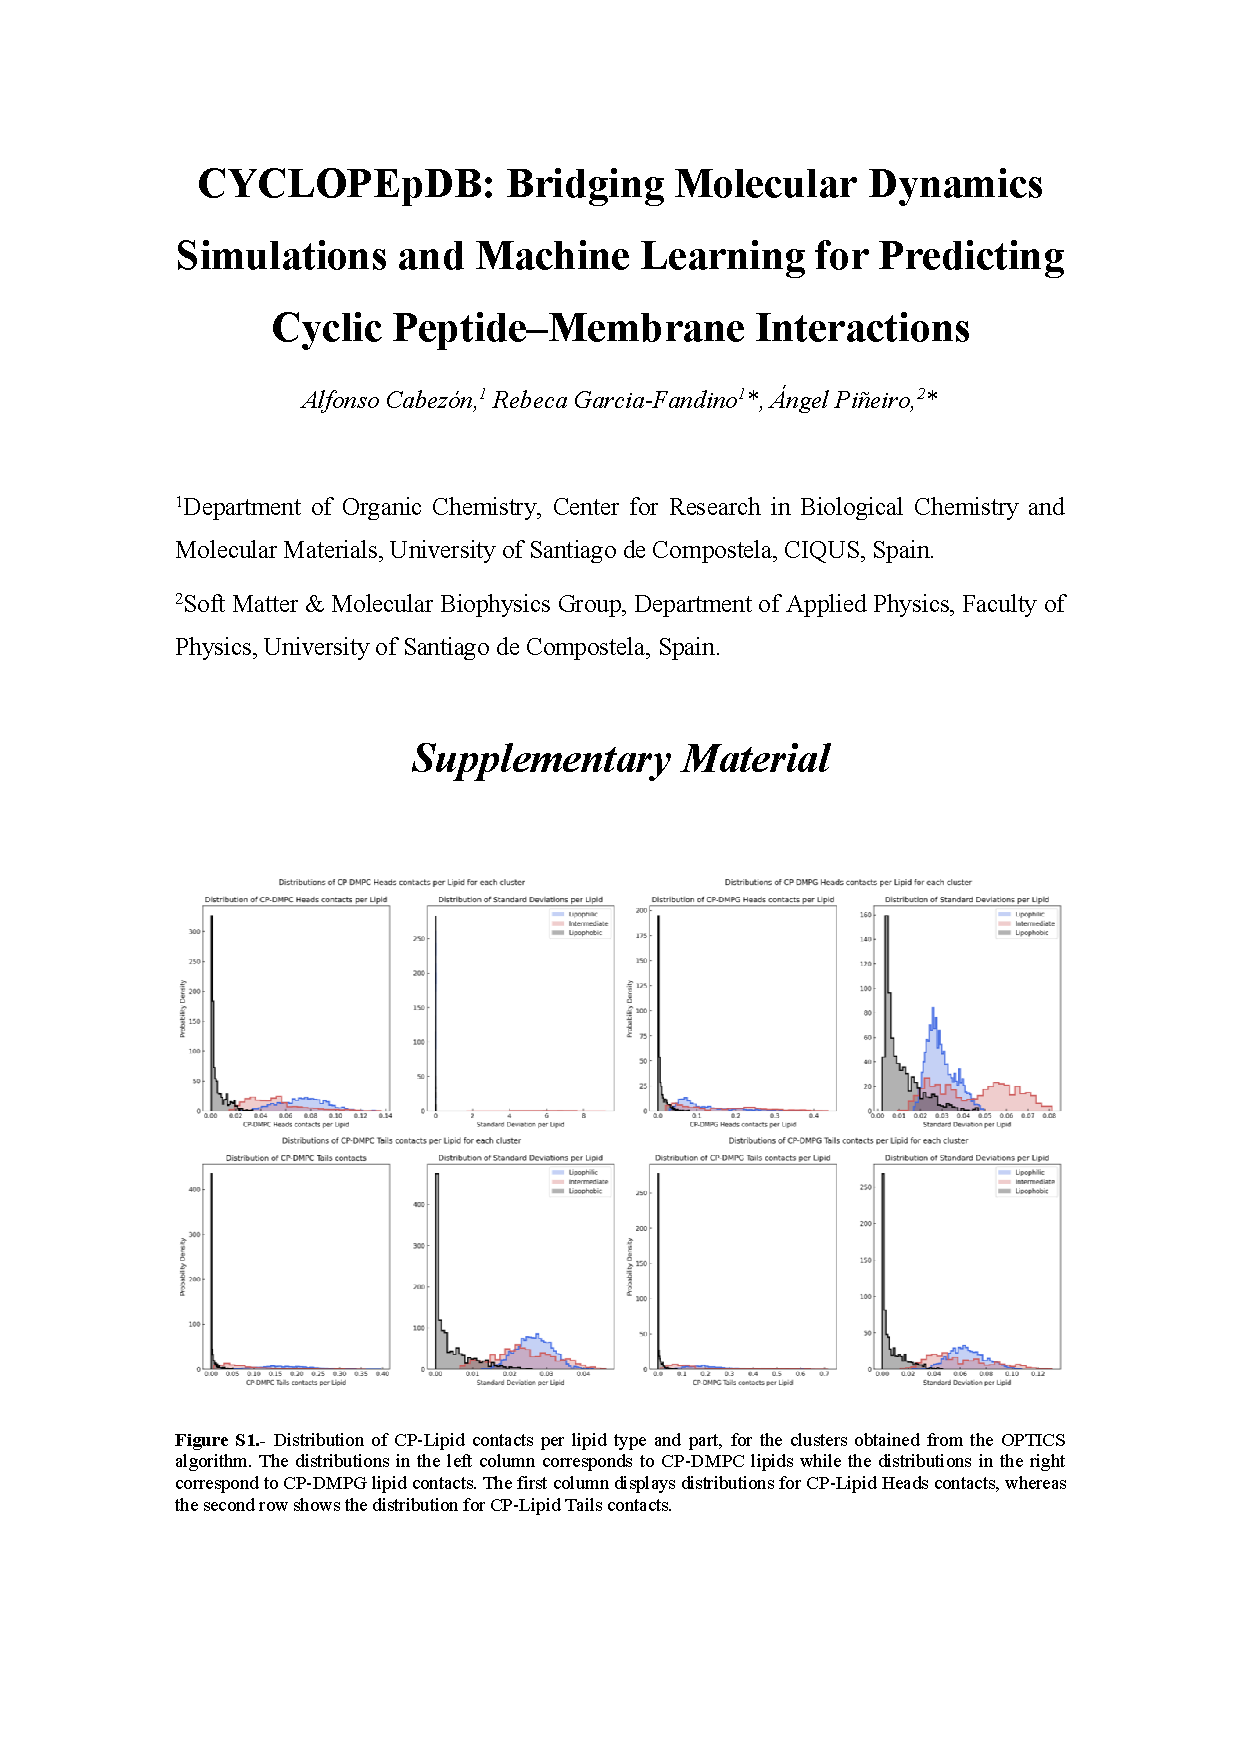
\includegraphics[page=1, width = \linewidth]{Appendix/Cabezon_2025_SI_final.pdf}

% \includepdf[pages=2-, width = 1.15\linewidth, pagecommand={\thispagestyle{fancy}}]{Appendix/Cabezon_2025_SI_final.pdf}

\section{Rights and Permissions for reproducing Images} % Use \section* instead of \chapter*

\begin{figure}[h!]
    \centering
    
\includegraphics[width=0.8\linewidth]{Appendix/Figures/Figure1.2.png}
    \caption{License of reproduction for Figure \ref{fig:AMPClass}}
    \label{fig:License 1}
\end{figure}

\begin{figure}[h!]
    \centering
    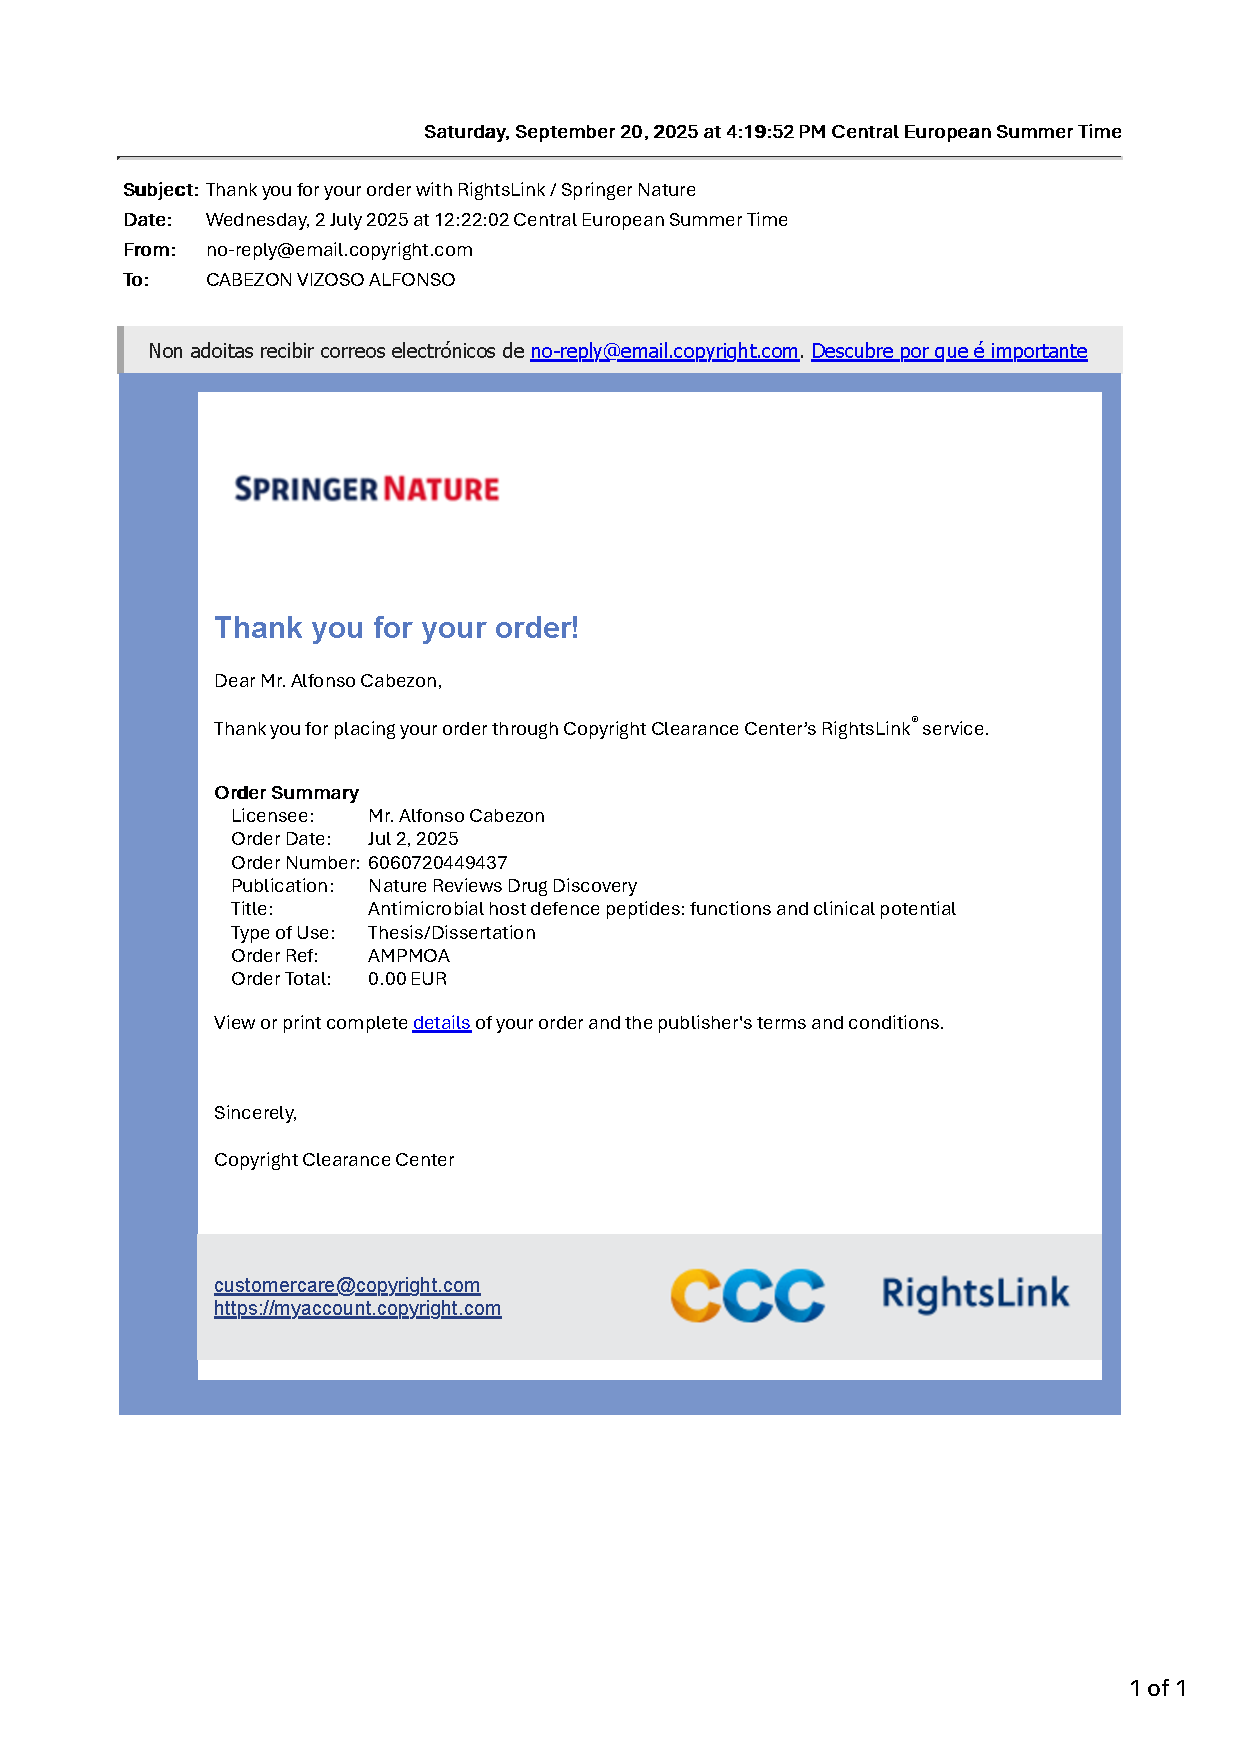
\includegraphics[width=0.6\linewidth, trim={0 5cm 0 2cm}, clip]{Appendix/Figures/License2.pdf}
    \caption{License of reproduction for Figure \ref{fig:AMPMOA}}
    \label{fig:License 2}
\end{figure}

\begin{figure}[h!]
    \centering
    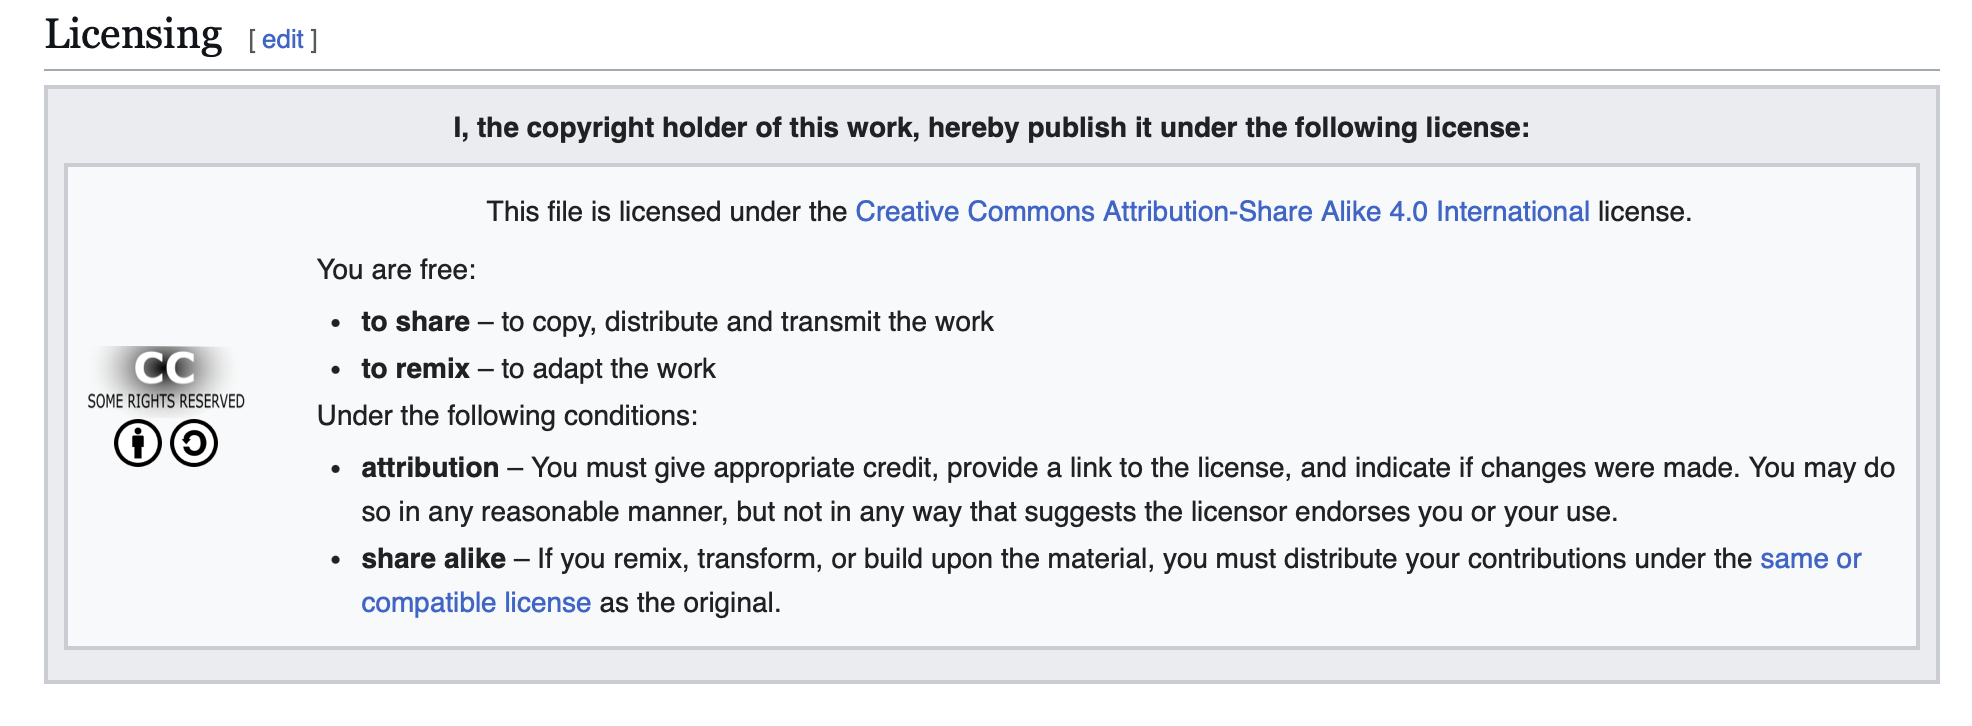
\includegraphics[width=0.8\linewidth]{Appendix/Figures/License3.6.png}
    \caption{License of reproduction for Figure \ref{fig:CNN}}
    \label{fig:License 3}
\end{figure}

\begin{figure}[h!]
    \centering
    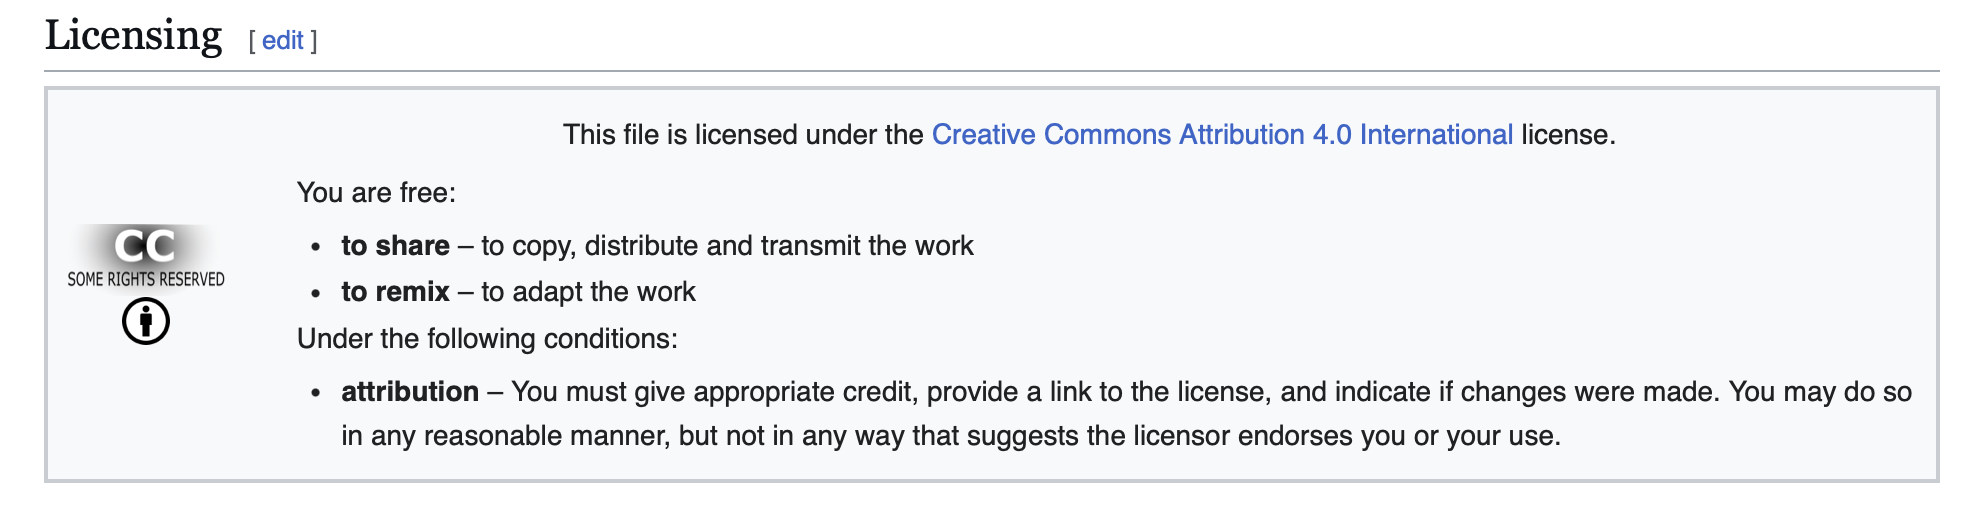
\includegraphics[width=0.8\linewidth]{Appendix/Figures/Figure3.8.png}
    \caption{License of reproduction for Figure \ref{fig:LSTM}}
    \label{fig:License 4}
\end{figure}

\section{Rights for reproduced content of published articles by the author}

\begin{figure}[h!]
    \centering
    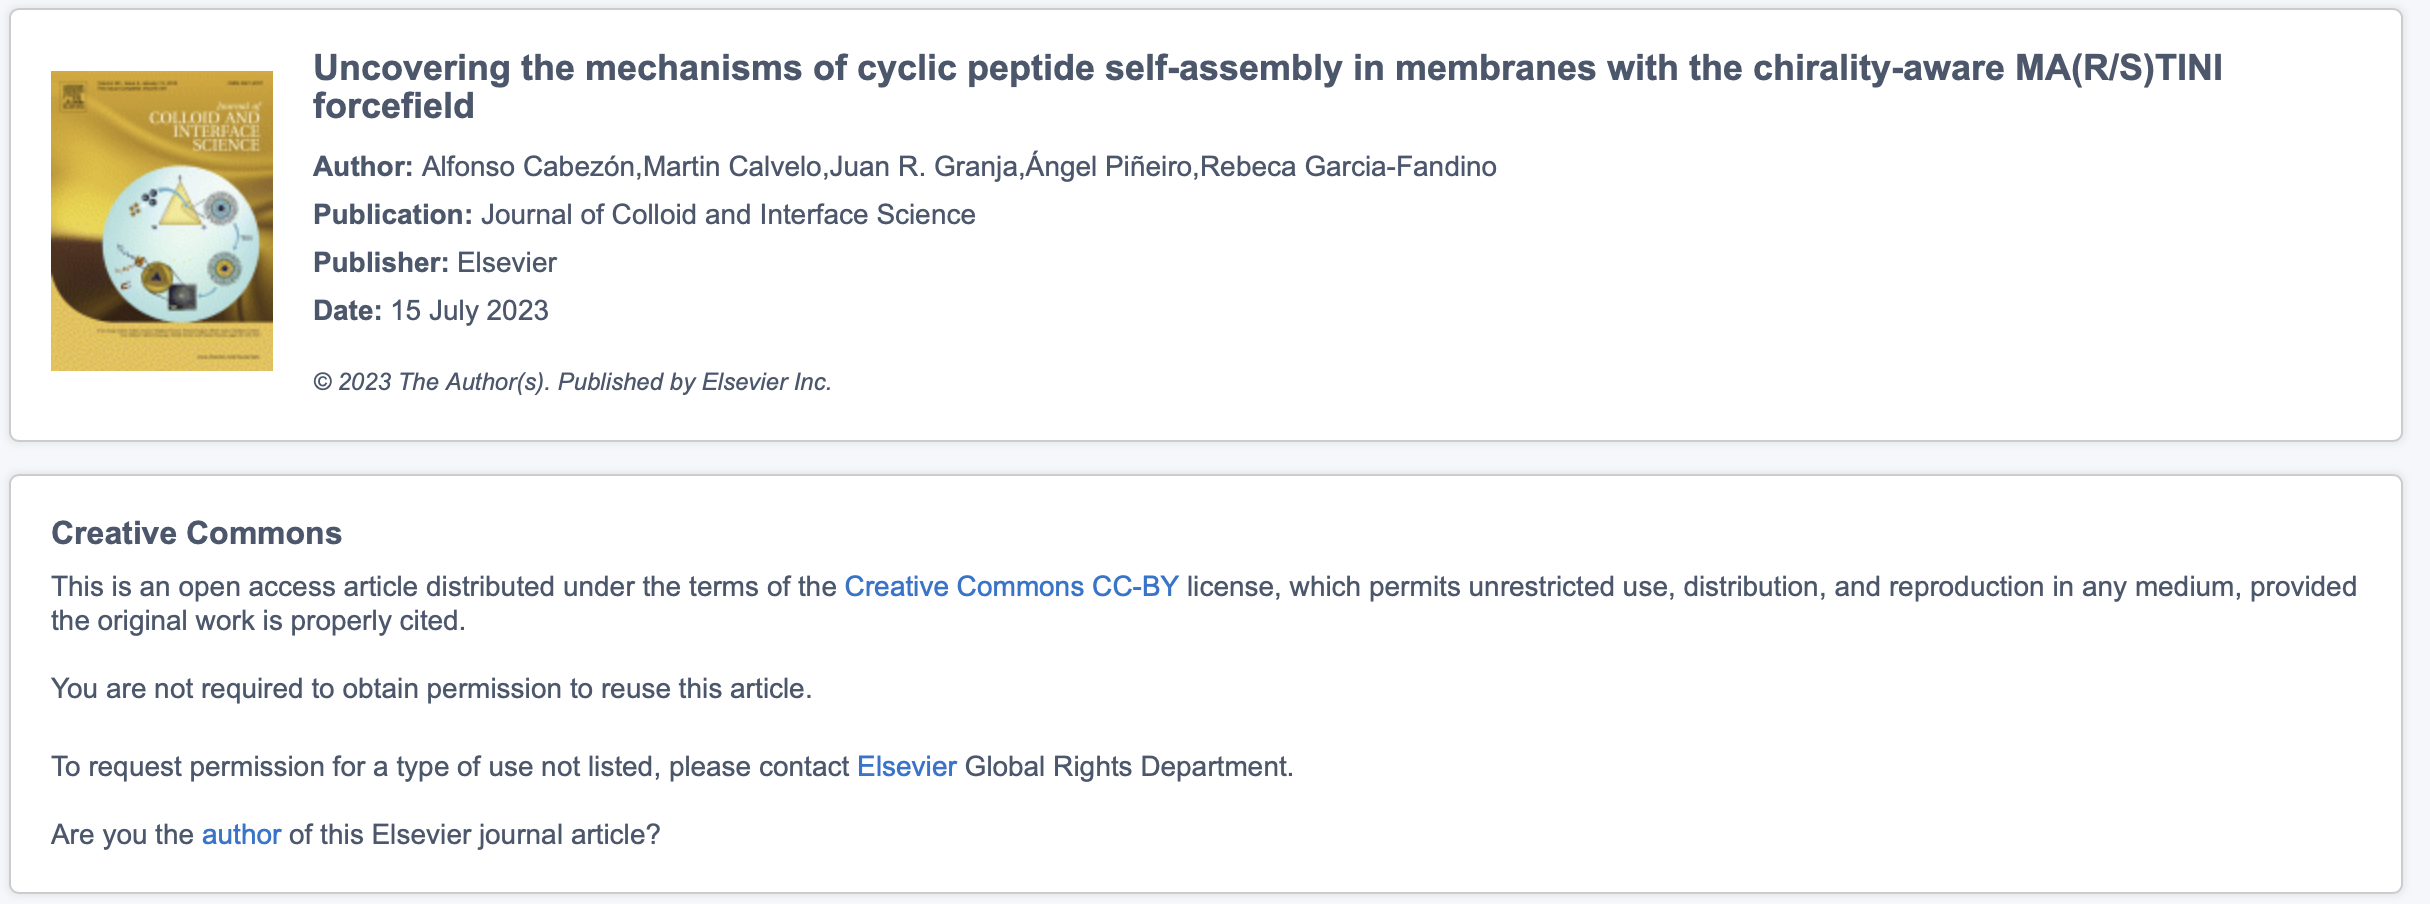
\includegraphics[width=\linewidth]{Appendix/Figures/PaperMARSTINI_Rights.png}
    \caption{License of reproduction for article in section \ref{art:MARSTINI}}
    \label{fig:License 5}
\end{figure}

\begin{figure}[h!]
    \centering
    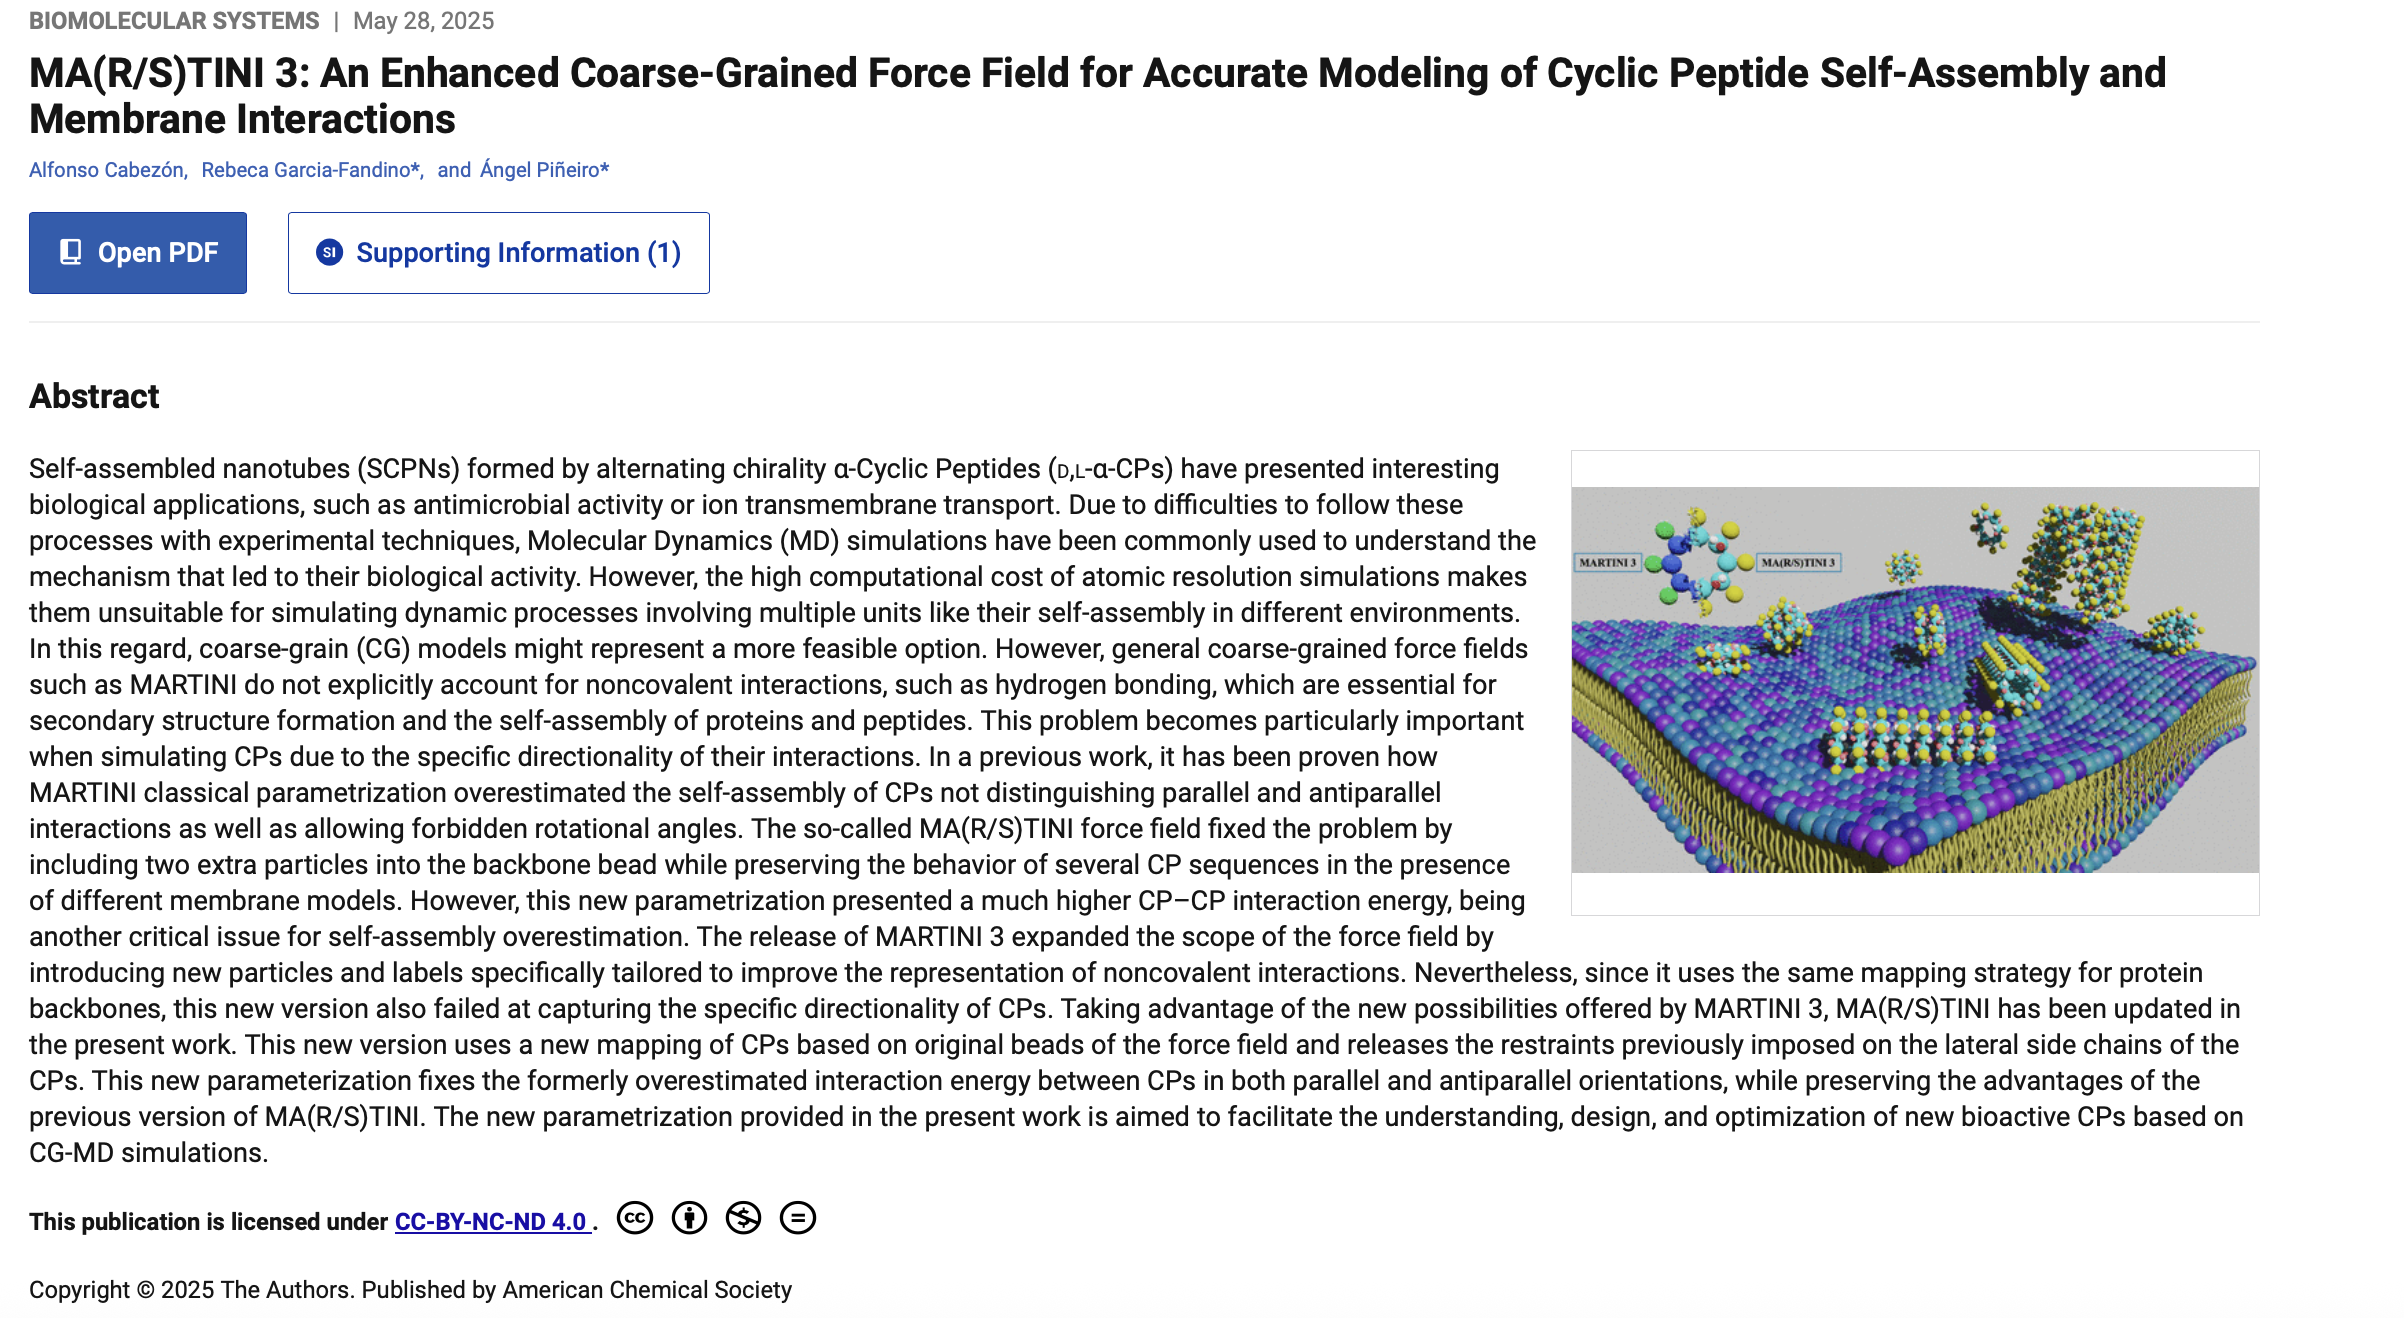
\includegraphics[width=0.8\linewidth]{Appendix/Figures/PaperMARSTINI3_Rights.png}
    \caption{License of reproduction for article in section \ref{art:MARSTINI3}}
    \label{fig:License 6}
\end{figure}

\begin{figure}[h!]
    \centering
    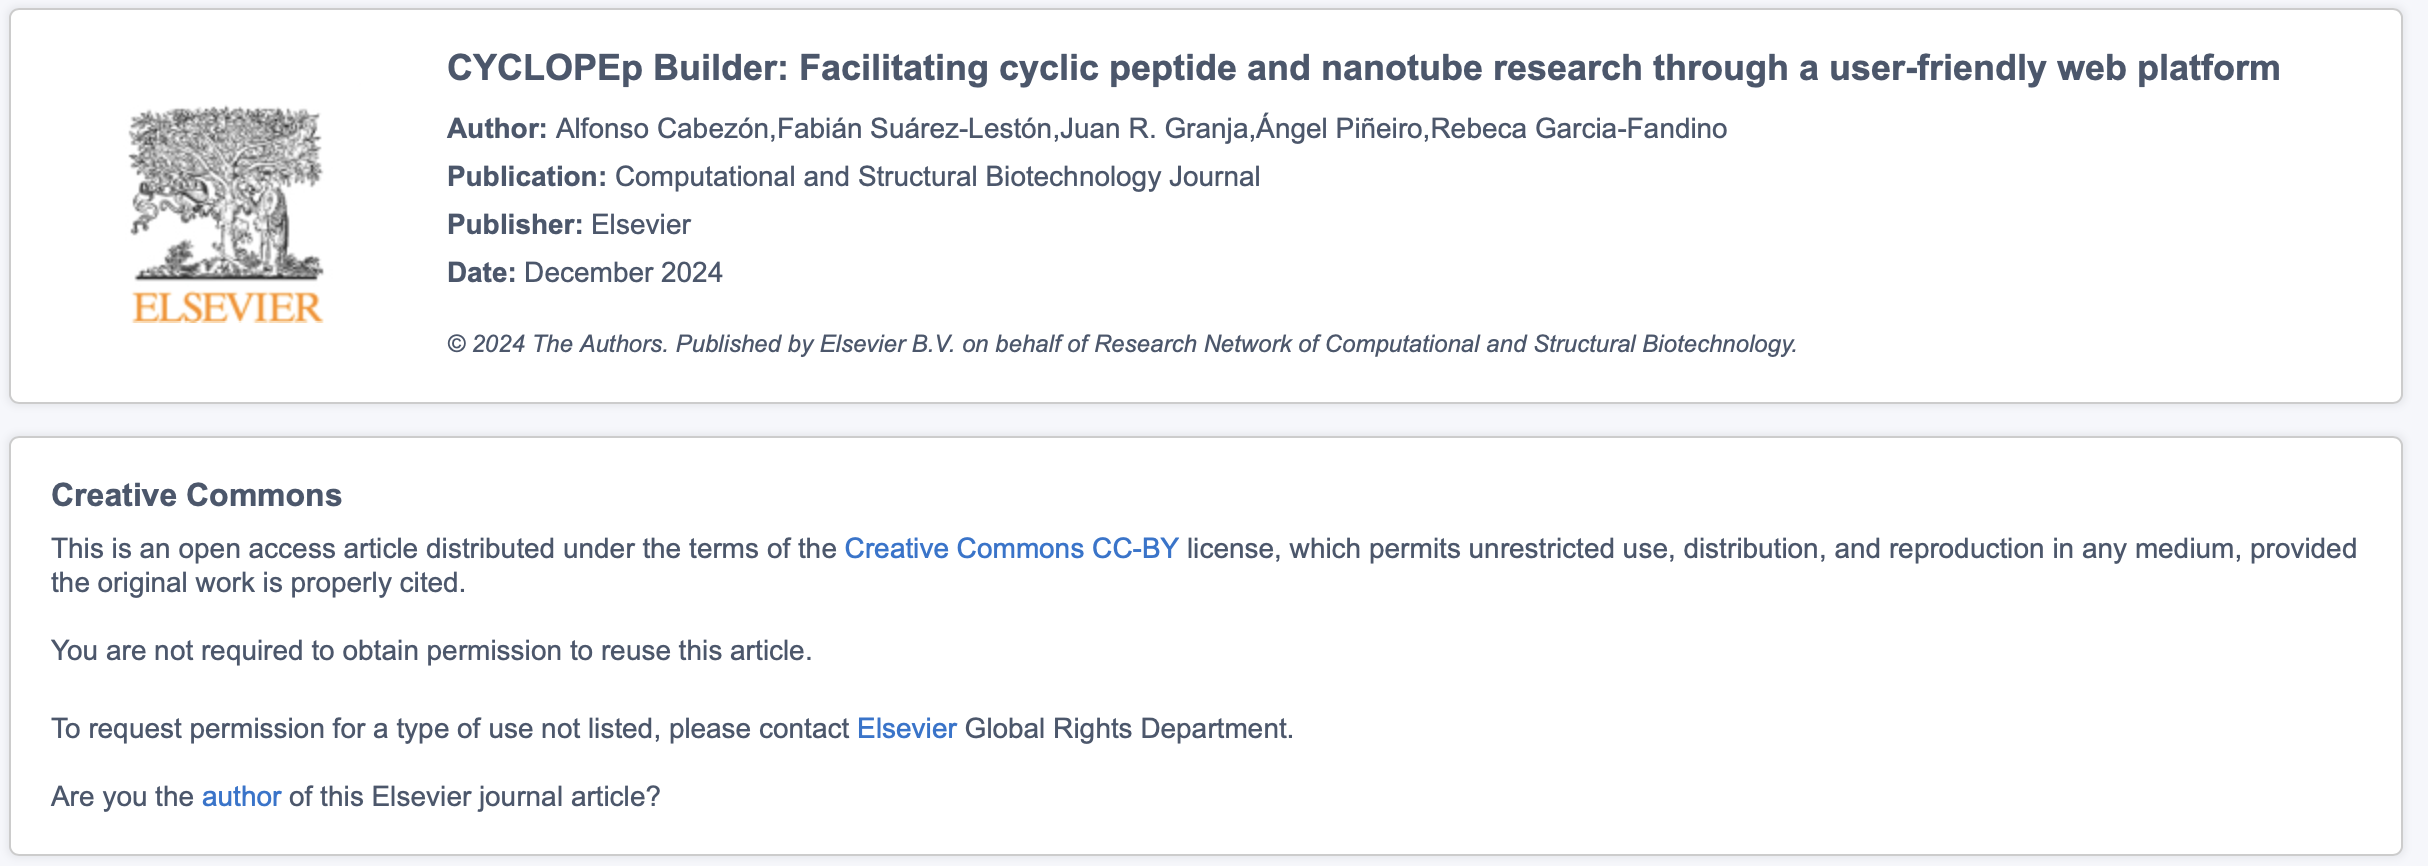
\includegraphics[width=\linewidth]{Appendix/Figures/CPBuilder_License.png}
    \caption{License of reproduction for article in section \ref{art:CPbuild}}
    \label{fig:License 7}
\end{figure}

\begin{figure}[h!]
    \centering
    
\includegraphics[width=\linewidth]{Appendix/Figures/CYCLOPs_Rights.png}
    \caption{License of reproduction for article in section \ref{art:CYCLOPs}}
    \label{fig:License 8}
\end{figure}






\includepdf[pages=-, pagecommand={\thispagestyle{empty}}]{Portada_Contraportada/Contraportada_tese.pdf} % Declaracion responsable

\end{document}
